\documentclass[a4paper]{article}

\usepackage{amsmath}
\usepackage{amssymb}
\usepackage{stellar}
\usepackage{parskip}
\usepackage{fullpage}
\usepackage{wrapfig}
\usepackage{enumitem}
\usepackage{tikz}
\usepackage{graphicx}
\usepackage{wrapfig}
\usepackage{circuitikz}
\usepackage{siunitx}
\usepackage{xcolor}
\usepackage{witharrows}
\usepackage{scalerel}

\usetikzlibrary{arrows}
\usetikzlibrary{cd}
\usetikzlibrary{decorations.pathmorphing}
\usetikzlibrary{decorations.markings}
\usetikzlibrary{decorations.pathreplacing}

\title{Lezioni di elettromagnetismo}
\author{Paolo Bettelini}
\date{}

%\pagecolor{black}
%\color{white}

\begin{document}

\maketitle
\tableofcontents

\part{Lezione 1}

\section{Introduzione all'elettrostatica}

L'elettromagnetismo studia i fenomeni dovuti alle cariche elettriche, alle correnti elettriche e ai campi elettrici e magnetici. Iniziamo dal caso più semplice: l'elettrostatica, cioè lo studio delle cariche ferme e dei campi elettrici da esse generati.

Dal punto di vista delle interazioni fondamentali, l'interazione elettromagnetica è una delle quattro forze fondamentali della natura. Ha lungo raggio d'azione e, su scala atomica e molecolare, è responsabile della coesione della materia ordinaria e delle interazioni tra atomi e molecole.

\begin{snippetproposition}{Confronto qualitativo tra interazioni fondamentali}
Le interazioni fondamentali principali sono:
\begin{itemize}
	\item l'interazione nucleare forte, intensa ma a cortissimo raggio, responsabile della coesione del nucleo;
	\item l'interazione elettromagnetica, a lungo raggio, che agisce tra cariche elettriche;
	\item l'interazione gravitazionale, a lungo raggio ma molto più debole dell'interazione elettromagnetica;
	\item l'interazione nucleare debole, a corto raggio, responsabile di alcuni decadimenti radioattivi.
\end{itemize}
\end{snippetproposition}

Storicamente, fenomeni elettrici e magnetici erano noti già dall'antichità. L'ambra strofinata può attirare piccoli corpi leggeri, mentre la magnetite attira la limatura di ferro. Questi fenomeni mostrano che la materia può esercitare forze a distanza, cioè senza contatto diretto.

\section{Elettrizzazione per strofinio}

Alcuni materiali, se strofinati, acquistano la capacità di attrarre o respingere altri corpi. Questo fenomeno si chiama elettrizzazione per strofinio.

I materiali possono comportarsi in modi diversi. Per esempio, vetro, ebanite, ambra, plastica e resine possono caricarsi durante lo strofinio. Sperimentalmente si osserva che:
\begin{itemize}
	\item corpi caricati nello stesso modo tendono a respingersi;
	\item corpi caricati in modi opposti tendono ad attrarsi.
\end{itemize}

\begin{snippetdefinition}{Carica elettrica positiva e negativa}
Esistono due tipi di carica elettrica, chiamati convenzionalmente positiva e negativa. Cariche dello stesso segno si respingono; cariche di segno opposto si attraggono.
\end{snippetdefinition}

\begin{center}
    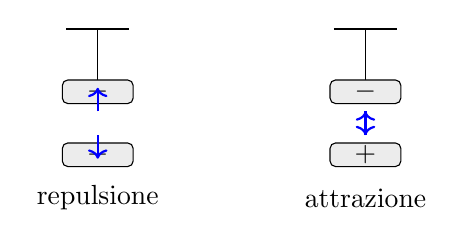
\begin{tikzpicture}[scale=1]
        \draw[thick] (-0.4,1.2) -- (0.4,1.2);
        \draw (0,1.2) -- (0,0.55);
        \draw[rounded corners=2pt,fill=gray!15] (-0.45,0.25) rectangle (0.45,0.55);
        \node at (0,0.4) {\( - \)};
        \draw[rounded corners=2pt,fill=gray!15] (-0.45,-0.55) rectangle (0.45,-0.25);
        \node at (0,-0.4) {\( - \)};
        \draw[->,blue,thick] (0,0.15) -- (0,0.45);
        \draw[->,blue,thick] (0,-0.15) -- (0,-0.45);
        \node at (0,-0.95) {repulsione};
        \draw[thick] (3.0,1.2) -- (3.8,1.2);
        \draw (3.4,1.2) -- (3.4,0.55);
        \draw[rounded corners=2pt,fill=gray!15] (2.95,0.25) rectangle (3.85,0.55);
        \node at (3.4,0.4) {\( - \)};
        \draw[rounded corners=2pt,fill=gray!15] (2.95,-0.55) rectangle (3.85,-0.25);
        \node at (3.4,-0.4) {\( + \)};
        \draw[->,blue,thick] (3.4,0.15) -- (3.4,-0.15);
        \draw[->,blue,thick] (3.4,-0.15) -- (3.4,0.15);
        \node at (3.4,-0.95) {attrazione};
    \end{tikzpicture}
\end{center}

\section{Struttura atomica della materia}

La descrizione moderna della materia spiega i fenomeni elettrici tramite la struttura atomica. Un atomo è formato da un nucleo centrale, contenente protoni e neutroni, e da elettroni che occupano regioni esterne al nucleo.

\begin{itemize}
	\item I protoni hanno carica positiva \(+e\).
	\item Gli elettroni hanno carica negativa \(-e\).
	\item I neutroni sono elettricamente neutri.
\end{itemize}

Il modulo della carica elementare è
\[
	e=1.6\cdot 10^{-19}\,\mathrm{C}.
\]
Un atomo neutro contiene lo stesso numero di protoni e di elettroni.

\begin{snippetdefinition}{Carica elementare}
La carica elementare \(e\) è il modulo della carica del protone e dell'elettrone:
\[
	e=1.6\cdot10^{-19}\,\mathrm{C}.
\]
Il protone ha carica \(+e\), mentre l'elettrone ha carica \(-e\).
\end{snippetdefinition}

\begin{center}
    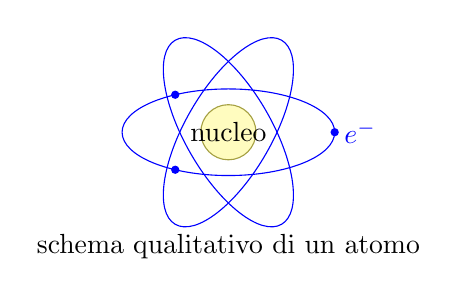
\begin{tikzpicture}[scale=1]
        \draw[fill=yellow!25,draw=yellow!60!black] (0,0) circle (0.35);
        \node at (0,0) {nucleo};
        \draw[blue] (0,0) ellipse (1.35 and 0.55);
        \draw[blue,rotate=60] (0,0) ellipse (1.35 and 0.55);
        \draw[blue,rotate=-60] (0,0) ellipse (1.35 and 0.55);
        \fill[blue] (1.35,0) circle (1.5pt) node[right] {\(e^-\)};
        \fill[blue] ({1.35*cos(120)},{0.55*sin(120)}) circle (1.5pt);
        \fill[blue] ({1.35*cos(240)},{0.55*sin(240)}) circle (1.5pt);
        \node at (0,-1.45) {schema qualitativo di un atomo};
    \end{tikzpicture}
\end{center}

Aggiungendo o togliendo elettroni da un atomo o da un corpo si ottiene una carica netta:
\begin{itemize}
	\item se si aggiungono elettroni, il corpo diventa carico negativamente;
	\item se si tolgono elettroni, il corpo diventa carico positivamente.
\end{itemize}

\begin{snippetdefinition}{Ione}
Un atomo o una molecola che ha perso o acquistato elettroni prende il nome di ione. Se perde elettroni diventa uno ione positivo; se acquista elettroni diventa uno ione negativo.
\end{snippetdefinition}

Le proprietà chimiche di un elemento sono determinate principalmente dal numero di protoni nel nucleo e dalla configurazione degli elettroni, in particolare degli elettroni più esterni.

\section{Isolanti e conduttori}

Il comportamento elettrico dei materiali dipende dalla possibilità degli elettroni di muoversi all'interno del materiale.

\begin{snippetdefinition}{Isolante}
Un isolante è un materiale in cui le cariche non sono libere di muoversi su distanze macroscopiche. Gli elettroni restano legati agli atomi o alle molecole.
\end{snippetdefinition}

\begin{snippetdefinition}{Conduttore}
Un conduttore è un materiale in cui alcune cariche sono libere di muoversi. Nei metalli le cariche mobili sono gli elettroni di conduzione.
\end{snippetdefinition}

La distinzione può essere interpretata qualitativamente in termini di bande di energia. Negli isolanti la banda di valenza è piena e separata dalla banda di conduzione da un grande intervallo di energia; nei conduttori, invece, esistono elettroni che possono muoversi facilmente e contribuire alla conduzione.

\begin{center}
    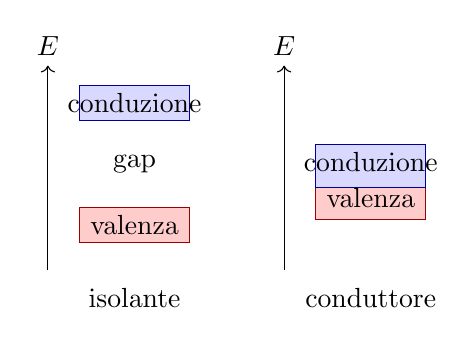
\begin{tikzpicture}[scale=1]
        \draw[->] (0,0) -- (0,2.6) node[above] {\(E\)};
        \draw[fill=red!20,draw=red!60!black] (0.4,0.35) rectangle (1.8,0.8);
        \draw[fill=blue!15,draw=blue!60!black] (0.4,1.9) rectangle (1.8,2.35);
        \node at (1.1,0.58) {valenza};
        \node at (1.1,2.12) {conduzione};
        \node at (1.1,1.35) {gap};
        \node at (1.1,-0.35) {isolante};
        \draw[->] (3.0,0) -- (3.0,2.6) node[above] {\(E\)};
        \draw[fill=red!20,draw=red!60!black] (3.4,0.65) rectangle (4.8,1.2);
        \draw[fill=blue!15,draw=blue!60!black] (3.4,1.05) rectangle (4.8,1.6);
        \node at (4.1,0.92) {valenza};
        \node at (4.1,1.38) {conduzione};
        \node at (4.1,-0.35) {conduttore};
    \end{tikzpicture}
\end{center}

\section{Induzione elettrostatica}

Consideriamo un corpo carico avvicinato a un conduttore neutro, senza toccarlo. Poiché nel conduttore gli elettroni possono muoversi, essi si ridistribuiscono sotto l'azione della forza elettrica.

Per esempio, se avviciniamo una bacchetta di plastica caricata negativamente a un conduttore neutro, gli elettroni del conduttore vengono respinti e si spostano verso la parte più lontana. La parte vicina alla bacchetta resta quindi con un eccesso di carica positiva, mentre la parte lontana presenta un eccesso di carica negativa. Il conduttore rimane complessivamente neutro, ma la carica non è distribuita uniformemente.

\begin{snippetdefinition}{Induzione elettrostatica}
L'induzione elettrostatica è la ridistribuzione delle cariche in un conduttore causata dalla presenza di un corpo carico vicino, senza contatto diretto.
\end{snippetdefinition}

\begin{center}
    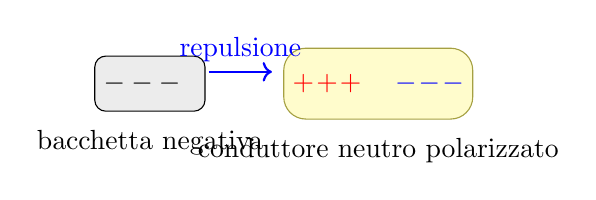
\begin{tikzpicture}[scale=1]
        \draw[rounded corners=4pt,fill=gray!15] (-1.7,-0.35) rectangle (-0.3,0.35);
        \foreach \x in {-1.45,-1.1,-0.75}{
            \node at (\x,0) {\(-\)};
        }
        \node at (-1.0,-0.75) {bacchetta negativa};
        \draw[rounded corners=8pt,fill=yellow!20,draw=yellow!60!black] (0.7,-0.45) rectangle (3.1,0.45);
        \foreach \x in {0.95,1.25,1.55}{
            \node[red] at (\x,0) {\(+\)};
        }
        \foreach \x in {2.25,2.55,2.85}{
            \node[blue] at (\x,0) {\(-\)};
        }
        \draw[->,blue,thick] (-0.25,0.15) -- (0.55,0.15) node[midway,above] {repulsione};
        \node at (1.9,-0.85) {conduttore neutro polarizzato};
    \end{tikzpicture}
\end{center}

La ridistribuzione avviene rapidamente e termina quando si raggiunge un equilibrio. In equilibrio, l'accumulo di carica prodotto dalla separazione impedisce un ulteriore spostamento netto degli elettroni.

\subsection{Carica per induzione e messa a terra}

Se, prima di allontanare la bacchetta carica, si collega il conduttore a terra, alcune cariche possono fluire verso o dalla Terra. Dopo aver rimosso il collegamento a terra e poi allontanato la bacchetta, il conduttore può rimanere carico.

\begin{center}
    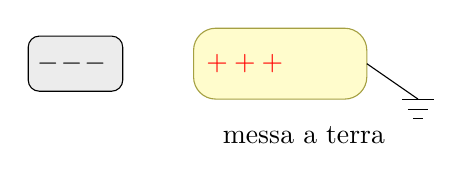
\begin{tikzpicture}[scale=1]
        \draw[rounded corners=4pt,fill=gray!15] (-1.5,-0.35) rectangle (-0.3,0.35);
        \foreach \x in {-1.25,-0.95,-0.65}{
            \node at (\x,0) {\(-\)};
        }
        \draw[rounded corners=8pt,fill=yellow!20,draw=yellow!60!black] (0.6,-0.45) rectangle (2.8,0.45);
        \foreach \x in {0.9,1.25,1.6}{
            \node[red] at (\x,0) {\(+\)};
        }
        \draw (2.8,0) -- (3.45,-0.45);
        \draw (3.25,-0.45) -- (3.65,-0.45);
        \draw (3.32,-0.58) -- (3.58,-0.58);
        \draw (3.39,-0.70) -- (3.51,-0.70);
        \node at (2.0,-0.9) {messa a terra};
    \end{tikzpicture}
\end{center}

\section{Forza elettrica e legge di Coulomb}

Il fatto che le cariche si attraggano o si respingano indica che tra cariche elettriche agisce una forza. Coulomb formulò quantitativamente questa forza.

Consideriamo due cariche puntiformi \(q_1\) e \(q_2\), separate da una distanza \(r\). Il modulo della forza elettrica è proporzionale al prodotto delle cariche e inversamente proporzionale al quadrato della distanza:
\[
	F\propto \frac{|q_1q_2|}{r^2}.
\]
La formula completa è
\[
	F=\frac{1}{4\pi\varepsilon_0}\frac{|q_1q_2|}{r^2}.
\]

\begin{snippettheorem}{Legge di Coulomb}
Due cariche puntiformi \(q_1\) e \(q_2\), poste a distanza \(r\), esercitano una sull'altra una forza di modulo
\[
	F=\frac{1}{4\pi\varepsilon_0}\frac{|q_1q_2|}{r^2}.
\]
La forza è diretta lungo la congiungente tra le due cariche: è repulsiva se \(q_1q_2>0\), attrattiva se \(q_1q_2<0\).
\end{snippettheorem}

\begin{center}
    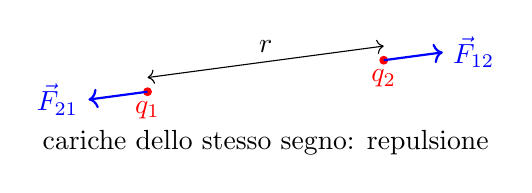
\begin{tikzpicture}[scale=1]
        \fill[red] (0,0) circle (1.6pt) node[below] {\(q_1\)};
        \fill[red] (3,0.4) circle (1.6pt) node[below] {\(q_2\)};
        \draw[<->] (0,0.18) -- (3,0.58) node[midway,above] {\(r\)};
        \draw[->,blue,thick] (0,0) -- (-0.75,-0.1) node[left] {\(\vec{F}_{21}\)};
        \draw[->,blue,thick] (3,0.4) -- (3.75,0.5) node[right] {\(\vec{F}_{12}\)};
        \node at (1.5,-0.65) {cariche dello stesso segno: repulsione};
    \end{tikzpicture}
\end{center}

La costante
\[
	\varepsilon_0=8.85\cdot10^{-12}\,\frac{\mathrm{C}^2}{\mathrm{N}\,\mathrm{m}^2}
\]
è la permittività elettrica del vuoto. Spesso si usa anche
\[
	\frac{1}{4\pi\varepsilon_0}\simeq 9\cdot10^9\,\frac{\mathrm{N}\,\mathrm{m}^2}{\mathrm{C}^2}.
\]

\section{Unità di misura della carica}

Nel Sistema Internazionale l'unità di misura della carica elettrica è il coulomb:
\[
	[ q ]=\mathrm{C}.
\]
Il coulomb è un'unità derivata. Per definizione operativa,
\[
	1\,\mathrm{C}=1\,\mathrm{A}\cdot1\,\mathrm{s}.
\]
Quindi un coulomb è la quantità di carica trasportata da una corrente di un ampere in un secondo.

La carica dell'elettrone è
\[
	-e=-1.6\cdot10^{-19}\,\mathrm{C}.
\]
Poiché la carica elementare è molto piccola, un coulomb corrisponde a un numero enorme di elettroni:
\[
	N=\frac{1\,\mathrm{C}}{1.6\cdot10^{-19}\,\mathrm{C}}
	\simeq 6\cdot10^{18}.
\]

\begin{snippetexample}{Ordine di grandezza della forza elettrica}
La carica indotta per strofinamento può essere dell'ordine di
\[
	q\sim 10^{-7}\,\mathrm{C}.
\]
Se due cariche di questo ordine sono poste a distanza
\[
	r=1\,\mathrm{cm}=10^{-2}\,\mathrm{m},
\]
la forza elettrica ha ordine di grandezza
\[
	F\simeq 9\cdot10^9\frac{(10^{-7})^2}{(10^{-2})^2}\,\mathrm{N}
	=9\cdot10^{-1}\,\mathrm{N}.
\]
Questa forza è facilmente misurabile.
\end{snippetexample}

\section{Forma vettoriale della legge di Coulomb}

La forza elettrica è un vettore: ha modulo, direzione e verso. Consideriamo la forza esercitata dalla carica \(q\) sulla carica di prova \(q_0\). Sia \(\vec{r}\) il vettore che va da \(q\) a \(q_0\), e sia
\[
	\hat{u}=\frac{\vec{r}}{|\vec{r}|}
\]
il versore lungo la congiungente.

Allora la forza su \(q_0\) è
\[
	\vec{F}=\frac{1}{4\pi\varepsilon_0}\frac{qq_0}{r^2}\hat{u}.
\]
Il segno del prodotto \(qq_0\) determina il verso della forza:
\begin{itemize}
	\item se \(qq_0>0\), la forza è repulsiva e ha verso \(\hat{u}\);
	\item se \(qq_0<0\), la forza è attrattiva e ha verso opposto a \(\hat{u}\).
\end{itemize}

\begin{snippetproposition}{Forma vettoriale della legge di Coulomb}
La forza esercitata da una carica puntiforme \(q\) su una carica \(q_0\) è
\[
	\vec{F}_{q\to q_0}=\frac{1}{4\pi\varepsilon_0}\frac{qq_0}{r^2}\hat{u},
\]
dove \(\hat{u}\) è il versore diretto da \(q\) verso \(q_0\).
\end{snippetproposition}

Per il principio di azione e reazione, la forza esercitata da \(q_0\) su \(q\) ha lo stesso modulo e verso opposto:
\[
	\vec{F}_{q_0\to q}=-\vec{F}_{q\to q_0}.
\]

\section{Principio di sovrapposizione per la forza elettrica}

Se una carica \(q_0\) è soggetta all'azione di molte cariche \(q_1,q_2,\dots,q_N\), la forza totale è la somma vettoriale delle forze dovute alle singole cariche.

Per tre cariche, per esempio,
\[
	\vec{F}_{\mathrm{tot}}=\vec{F}_1+\vec{F}_2+\vec{F}_3.
\]
In componenti:
\[
	F_{\mathrm{tot},x}=F_{1,x}+F_{2,x}+F_{3,x},
	\qquad
	F_{\mathrm{tot},y}=F_{1,y}+F_{2,y}+F_{3,y},
	\qquad
	F_{\mathrm{tot},z}=F_{1,z}+F_{2,z}+F_{3,z}.
\]

Più in generale,
\[
	\vec{F}_{\mathrm{tot}}=\sum_{i=1}^N\vec{F}_i.
\]
Per ogni carica \(q_i\), si ha
\[
	\vec{F}_i=\frac{1}{4\pi\varepsilon_0}\frac{q_iq_0}{r_i^2}\hat{u}_i.
\]
Quindi
\[
	\vec{F}_{\mathrm{tot}}
	=\frac{q_0}{4\pi\varepsilon_0}\sum_{i=1}^N\frac{q_i}{r_i^2}\hat{u}_i.
\]

\begin{snippettheorem}{Principio di sovrapposizione}
La forza totale esercitata da un sistema di cariche puntiformi \(q_1,\dots,q_N\) su una carica \(q_0\) è la somma vettoriale delle forze esercitate da ciascuna carica:
\[
	\vec{F}_{\mathrm{tot}}=\sum_{i=1}^N\vec{F}_i
	=\frac{q_0}{4\pi\varepsilon_0}\sum_{i=1}^N\frac{q_i}{r_i^2}\hat{u}_i.
\]
\end{snippettheorem}

\begin{center}
    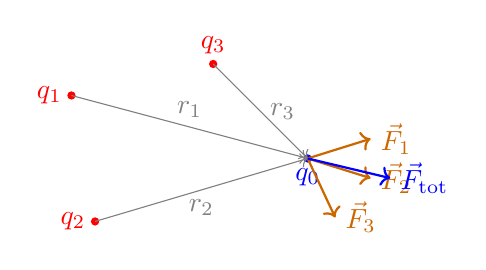
\begin{tikzpicture}[scale=1]
        \fill[red] (-1.8,0.8) circle (1.5pt) node[left] {\(q_1\)};
        \fill[red] (-1.5,-0.8) circle (1.5pt) node[left] {\(q_2\)};
        \fill[red] (0.0,1.2) circle (1.5pt) node[above] {\(q_3\)};
        \fill[blue] (1.2,0) circle (1.5pt) node[below] {\(q_0\)};
        \draw[->,gray] (-1.8,0.8) -- (1.2,0) node[midway,above] {\(r_1\)};
        \draw[->,gray] (-1.5,-0.8) -- (1.2,0) node[midway,below] {\(r_2\)};
        \draw[->,gray] (0.0,1.2) -- (1.2,0) node[midway,right] {\(r_3\)};
        \draw[->,orange!80!black,thick] (1.2,0) -- (2.0,0.25) node[right] {\(\vec{F}_1\)};
        \draw[->,orange!80!black,thick] (1.2,0) -- (2.0,-0.25) node[right] {\(\vec{F}_2\)};
        \draw[->,orange!80!black,thick] (1.2,0) -- (1.55,-0.75) node[right] {\(\vec{F}_3\)};
        \draw[->,blue,thick] (1.2,0) -- (2.25,-0.25) node[right] {\(\vec{F}_{\mathrm{tot}}\)};
    \end{tikzpicture}
\end{center}

La forza totale è proporzionale alla carica di prova \(q_0\). Questo fatto permette di introdurre il campo elettrostatico.

\section{Campo elettrostatico}

Prendiamo una carica di prova \(q_0\) piccola, in modo che la sua presenza non modifichi sensibilmente la distribuzione sorgente. Se il sistema di cariche \(q_1,q_2,\dots,q_N\) esercita su \(q_0\) una forza totale \(\vec{F}\), definiamo il campo elettrostatico come
\[
	\vec{E}=\frac{\vec{F}}{q_0}.
\]
Equivalentemente,
\[
	\vec{F}=q_0\vec{E}.
\]

\begin{snippetdefinition}{Campo elettrostatico}
Il campo elettrostatico in un punto \(P\), prodotto da un sistema di cariche ferme, è la forza elettrostatica che una carica di prova \(q_0\) sentirebbe nel punto \(P\), divisa per \(q_0\):
\[
	\vec{E}(P)=\frac{\vec{F}(P)}{q_0}.
\]
\end{snippetdefinition}

Per una sola carica puntiforme \(q_1\), il campo nel punto \(P\) è
\[
	\vec{E}(P)=\frac{1}{4\pi\varepsilon_0}\frac{q_1}{r^2}\hat{u}.
\]
Il verso dipende dal segno di \(q_1\): se \(q_1>0\), il campo è uscente dalla carica; se \(q_1<0\), il campo è entrante verso la carica.

\begin{center}
    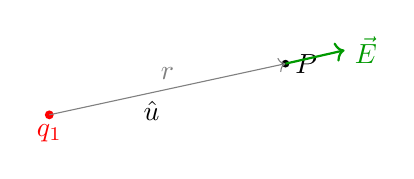
\begin{tikzpicture}[scale=1]
        \fill[red] (0,0) circle (1.6pt) node[below] {\(q_1\)};
        \fill (3.0,0.65) circle (1.4pt) node[right] {\(P\)};
        \draw[->,gray] (0,0) -- (3.0,0.65) node[midway,above] {\(r\)};
        \draw[->,green!60!black,thick] (3.0,0.65) -- (3.75,0.82) node[right] {\(\vec{E}\)};
        \node at (1.3,0.05) {\(\hat{u}\)};
    \end{tikzpicture}
\end{center}

Per un sistema di cariche puntiformi, dalla formula della forza totale segue immediatamente
\[
	\vec{E}(P)=\frac{1}{4\pi\varepsilon_0}\sum_{i=1}^N\frac{q_i}{r_i^2}\hat{u}_i.
\]

\begin{snippettheorem}{Campo elettrostatico generato da cariche puntiformi}
Il campo elettrostatico generato da \(N\) cariche puntiformi ferme è
\[
	\vec{E}(P)=\frac{1}{4\pi\varepsilon_0}\sum_{i=1}^N\frac{q_i}{r_i^2}\hat{u}_i.
\]
\end{snippettheorem}

\pagebreak
\part{Lezione 2}

\section{Campi vettoriali e campo elettrico}

Un campo vettoriale associa a ogni punto dello spazio un vettore. Per esempio, in due dimensioni possiamo avere
\[
	\vec{A}=\vec{A}(x,y),
\]
mentre in tre dimensioni
\[
	\vec{A}=\vec{A}(x,y,z).
\]
Il vettore assegnato può cambiare da punto a punto in modulo, direzione e verso.

\begin{snippetdefinition}{Campo vettoriale}
Un campo vettoriale nello spazio è una funzione che associa a ogni punto \(P=(x,y,z)\) un vettore:
\[
	P\longmapsto \vec{A}(P)=\vec{A}(x,y,z).
\]
\end{snippetdefinition}

\begin{center}
    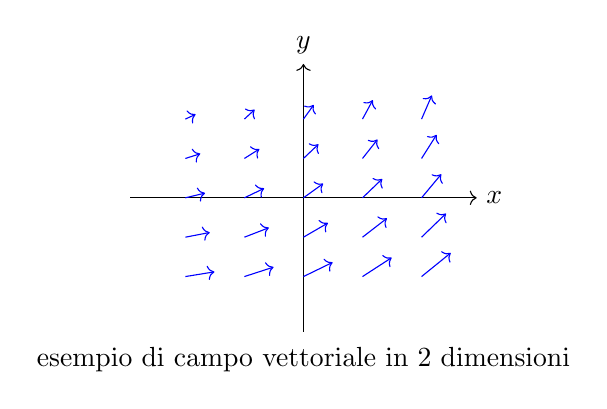
\begin{tikzpicture}[scale=1]
        \draw[->] (-2.2,0) -- (2.2,0) node[right] {\(x\)};
        \draw[->] (0,-1.7) -- (0,1.7) node[above] {\(y\)};
        \foreach \x in {-1.5,-0.75,0,0.75,1.5}{
            \foreach \y in {-1.0,-0.5,0,0.5,1.0}{
                \draw[->,blue] (\x,\y) -- ++({0.25-0.12*\y},{0.18+0.08*\x});
            }
        }
        \node at (0,-2.05) {esempio di campo vettoriale in \(2\) dimensioni};
    \end{tikzpicture}
\end{center}

Un esempio fisico importante è il campo gravitazionale. Una massa modifica lo spazio circostante: un'altra massa posta nelle vicinanze risente di una forza gravitazionale. In modo analogo, una distribuzione di carica genera un campo elettrico nello spazio circostante; una carica posta in un punto dello spazio risente poi della forza elettrica dovuta a quel campo.

\section{Definizione di campo elettrico}

Consideriamo una distribuzione di cariche sorgenti. Mettiamo una carica di prova \(q_0\) nel punto \(P\). Se la forza elettrica esercitata dalla distribuzione su \(q_0\) è \(\vec{F}(P)\), definiamo il campo elettrico in \(P\) come
\[
	\vec{E}(P)=\frac{\vec{F}(P)}{q_0}.
\]
Quindi
\[
	\vec{F}(P)=q_0\vec{E}(P).
\]

\begin{snippetdefinition}{Campo elettrico}
Il campo elettrico generato da una distribuzione di carica è la forza elettrica per unità di carica di prova:
\[
	\vec{E}=\frac{\vec{F}}{q_0}.
\]
La sua unità di misura è
\[
	[\vec{E}]=\frac{\mathrm{N}}{\mathrm{C}}.
\]
\end{snippetdefinition}

La carica di prova serve solo per misurare il campo. Il campo elettrico è una proprietà della distribuzione sorgente e del punto dello spazio considerato, non della carica di prova.

\section{Campo generato da una carica puntiforme}

Sia \(q\) una carica puntiforme. Una carica di prova \(q_0\), posta a distanza \(r\), subisce la forza di Coulomb
\[
	\vec{F}=\frac{1}{4\pi\varepsilon_0}\frac{qq_0}{r^2}\hat{u},
\]
dove \(\hat{u}\) è il versore diretto dalla carica sorgente al punto in cui si trova la carica di prova.

Dividendo per \(q_0\), otteniamo il campo elettrico:
\[
	\vec{E}=\frac{\vec{F}}{q_0}
	=\frac{1}{4\pi\varepsilon_0}\frac{q}{r^2}\hat{u}.
\]

\begin{snippettheorem}{Campo elettrico di una carica puntiforme}
Il campo elettrico generato da una carica puntiforme \(q\) è
\[
	\vec{E}(P)=\frac{1}{4\pi\varepsilon_0}\frac{q}{r^2}\hat{u},
\]
dove \(r\) è la distanza tra la carica e il punto \(P\), e \(\hat{u}\) è il versore diretto dalla carica verso \(P\).
\end{snippettheorem}

\begin{center}
    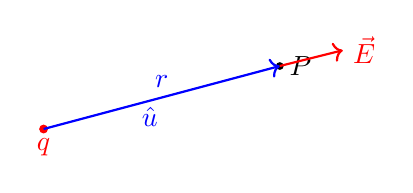
\begin{tikzpicture}[scale=1]
        \fill[red] (0,0) circle (1.6pt) node[below] {\(q\)};
        \fill (3,0.8) circle (1.4pt) node[right] {\(P\)};
        \draw[->,blue,thick] (0,0) -- (3,0.8) node[midway,above] {\(r\)};
        \draw[->,red,thick] (3,0.8) -- (3.8,1.0) node[right] {\(\vec{E}\)};
        \node[blue] at (1.35,0.15) {\(\hat{u}\)};
    \end{tikzpicture}
\end{center}

Se \(q>0\), il campo è uscente dalla carica; se \(q<0\), il campo è entrante verso la carica.

\section{Principio di sovrapposizione}

Consideriamo ora \(N\) cariche puntiformi \(q_1,q_2,\dots,q_N\). Il campo nel punto \(P\) è la somma vettoriale dei campi prodotti dalle singole cariche:
\[
	\vec{E}(P)=\sum_{i=1}^N\vec{E}_i(P).
\]
Per ogni carica
\[
	\vec{E}_i(P)=\frac{1}{4\pi\varepsilon_0}\frac{q_i}{r_i^2}\hat{u}_i,
\]
dove \(r_i\) è la distanza tra \(q_i\) e \(P\), e \(\hat{u}_i\) è il versore diretto da \(q_i\) verso \(P\). Dunque
\[
	\vec{E}(P)=\frac{1}{4\pi\varepsilon_0}\sum_{i=1}^N\frac{q_i}{r_i^2}\hat{u}_i.
\]

\begin{snippettheorem}{Principio di sovrapposizione per il campo elettrico}
Il campo elettrico generato da una distribuzione discreta di cariche è
\[
	\vec{E}(P)=\frac{1}{4\pi\varepsilon_0}\sum_{i=1}^N\frac{q_i}{r_i^2}\hat{u}_i.
\]
Il campo totale è la somma vettoriale dei contributi di tutte le cariche.
\end{snippettheorem}

Se \(P=(x_P,y_P,z_P)\), il campo in \(P\) può essere scritto anche in componenti:
\[
	\vec{E}(P)=E_x(P)\hat{x}+E_y(P)\hat{y}+E_z(P)\hat{z}.
\]
La forza su una carica \(q_0\) posta in \(P\) è quindi
\[
	\vec{F}(P)=q_0\vec{E}(P).
\]

\begin{center}
    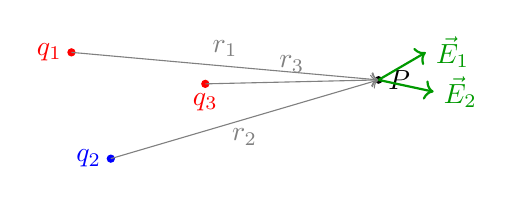
\begin{tikzpicture}[scale=1]
        \fill[red] (-1.2,0.6) circle (1.5pt) node[left] {\(q_1\)};
        \fill[blue] (-0.7,-0.75) circle (1.5pt) node[left] {\(q_2\)};
        \fill[red] (0.5,0.2) circle (1.5pt) node[below] {\(q_3\)};
        \fill (2.7,0.25) circle (1.4pt) node[right] {\(P\)};
        \draw[->,gray] (-1.2,0.6) -- (2.7,0.25) node[midway,above] {\(r_1\)};
        \draw[->,gray] (-0.7,-0.75) -- (2.7,0.25) node[midway,below] {\(r_2\)};
        \draw[->,gray] (0.5,0.2) -- (2.7,0.25) node[midway,above] {\(r_3\)};
        \draw[->,green!60!black,thick] (2.7,0.25) -- (3.3,0.6) node[right] {\(\vec{E}_1\)};
        \draw[->,green!60!black,thick] (2.7,0.25) -- (3.4,0.1) node[right] {\(\vec{E}_2\)};
    \end{tikzpicture}
\end{center}

\section{Linee di forza del campo elettrico}

Le linee di forza sono un modo geometrico per rappresentare un campo elettrico. Esse non sono oggetti materiali: sono curve disegnate in modo da visualizzare direzione, verso e intensità del campo.

\begin{snippetdefinition}{Linee di forza del campo elettrico}
Le linee di forza del campo elettrico sono curve tali che, in ogni punto, il vettore \(\vec{E}\) è tangente alla curva e concorde con il suo verso.
\end{snippetdefinition}

Le linee di forza hanno alcune proprietà fondamentali:
\begin{itemize}
	\item sono tangenti e concordi con \(\vec{E}\) in ogni punto;
	\item sono più fitte dove il campo è più intenso;
	\item non si intrecciano mai, perché in ogni punto il campo elettrico ha una sola direzione;
	\item escono dalle cariche positive ed entrano nelle cariche negative.
\end{itemize}

Se è presente una sola carica positiva, le linee escono dalla carica e si estendono fino all'infinito. Se è presente una sola carica negativa, le linee arrivano dall'infinito ed entrano nella carica.

\begin{center}
    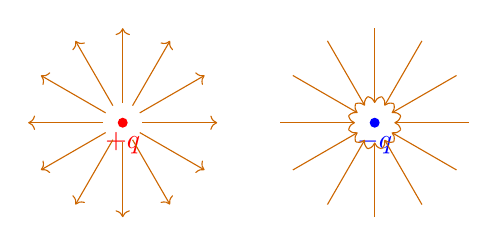
\begin{tikzpicture}[scale=1]
        \fill[red] (0,0) circle (1.8pt) node[below] {\(+q\)};
        \foreach \a in {0,30,...,330}{
            \draw[->,orange!80!black] ({0.25*cos(\a)},{0.25*sin(\a)}) -- ({1.2*cos(\a)},{1.2*sin(\a)});
        }
        \fill[blue] (3.2,0) circle (1.8pt) node[below] {\(-q\)};
        \foreach \a in {0,30,...,330}{
            \draw[->,orange!80!black] ({3.2+1.2*cos(\a)},{1.2*sin(\a)}) -- ({3.2+0.25*cos(\a)},{0.25*sin(\a)});
        }
    \end{tikzpicture}
\end{center}

\subsection{Esempi di linee di campo}

Per due cariche opposte, le linee partono dalla carica positiva e terminano sulla carica negativa.

\begin{center}
    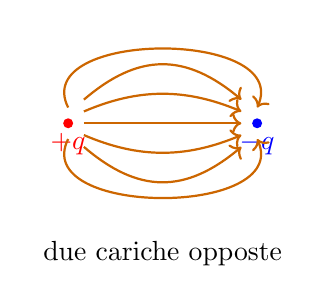
\begin{tikzpicture}[scale=1]
        \fill[red] (-1.2,0) circle (1.8pt) node[below] {\(+q\)};
        \fill[blue] (1.2,0) circle (1.8pt) node[below] {\(-q\)};
        \foreach \y in {-0.9,-0.45,0,0.45,0.9}{
            \draw[->,orange!80!black,thick] (-1.0,\y/3) .. controls (-0.3,\y) and (0.3,\y) .. (1.0,\y/3);
        }
        \draw[->,orange!80!black,thick] (-1.2,0.2) .. controls (-1.7,1.2) and (1.7,1.2) .. (1.2,0.2);
        \draw[->,orange!80!black,thick] (-1.2,-0.2) .. controls (-1.7,-1.2) and (1.7,-1.2) .. (1.2,-0.2);
        \node at (0,-1.65) {due cariche opposte};
    \end{tikzpicture}
\end{center}

Per due cariche dello stesso segno, le linee escono da entrambe e si deformano a causa della repulsione reciproca.

\begin{center}
    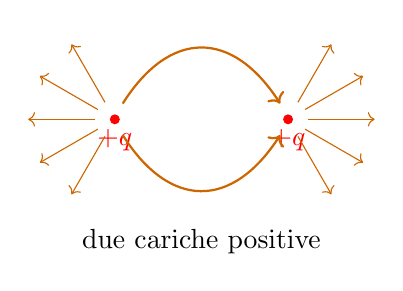
\begin{tikzpicture}[scale=1]
        \fill[red] (-1.1,0) circle (1.8pt) node[below] {\(+q\)};
        \fill[red] (1.1,0) circle (1.8pt) node[below] {\(+q\)};
        \foreach \a in {120,150,180,210,240}{
            \draw[->,orange!80!black] ({-1.1+0.25*cos(\a)},{0.25*sin(\a)}) -- ({-1.1+1.1*cos(\a)},{1.1*sin(\a)});
        }
        \foreach \a in {-60,-30,0,30,60}{
            \draw[->,orange!80!black] ({1.1+0.25*cos(\a)},{0.25*sin(\a)}) -- ({1.1+1.1*cos(\a)},{1.1*sin(\a)});
        }
        \draw[->,orange!80!black,thick] (-1.0,0.2) .. controls (-0.4,1.15) and (0.4,1.15) .. (1.0,0.2);
        \draw[->,orange!80!black,thick] (-1.0,-0.2) .. controls (-0.4,-1.15) and (0.4,-1.15) .. (1.0,-0.2);
        \node at (0,-1.55) {due cariche positive};
    \end{tikzpicture}
\end{center}

\section{Campo elettrico di un piano carico: simmetria}

Consideriamo un piano uniformemente carico. Per simmetria, il campo elettrico deve essere perpendicolare al piano. Infatti, presi due elementi simmetrici della distribuzione, le componenti parallele al piano si cancellano, mentre le componenti perpendicolari si sommano.

\begin{center}
    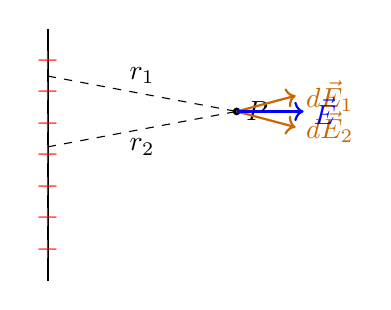
\begin{tikzpicture}[scale=1]
        \draw[thick] (0,-1.6) -- (0,1.6);
        \foreach \y in {-1.2,-0.8,-0.4,0,0.4,0.8,1.2}{
            \node[red] at (0,\y) {\(+\)};
        }
        \fill (2.4,0.55) circle (1.4pt) node[right] {\(P\)};
        \draw[dashed] (0,1.0) -- (2.4,0.55) node[midway,above] {\(r_1\)};
        \draw[dashed] (0,0.1) -- (2.4,0.55) node[midway,below] {\(r_2\)};
        \draw[->,orange!80!black,thick] (2.4,0.55) -- (3.15,0.75) node[right] {\(d\vec{E}_1\)};
        \draw[->,orange!80!black,thick] (2.4,0.55) -- (3.15,0.35) node[right] {\(d\vec{E}_2\)};
        \draw[->,blue,thick] (2.4,0.55) -- (3.25,0.55) node[right] {\(\vec{E}\)};
    \end{tikzpicture}
\end{center}

Inoltre, per un piano infinito uniformemente carico, la densità delle linee di campo non cambia allontanandosi dal piano. Questo suggerisce che il modulo del campo sia costante e non dipenda dalla distanza dal piano. Il calcolo preciso verrà fatto con la legge di Gauss, ma la simmetria permette già di capire la direzione del campo.

\begin{snippetproposition}{Campo di un piano infinito carico}
Il campo elettrico generato da un piano infinito uniformemente carico è perpendicolare al piano e ha modulo costante, indipendente dalla distanza dal piano.
\end{snippetproposition}

\section{Moto di una carica in un campo elettrico}

Una volta noto il campo elettrico \(\vec{E}\), il moto di una carica \(q\) al suo interno si studia con la seconda legge di Newton. La forza elettrica è
\[
	\vec{F}=q\vec{E}.
\]
Quindi
\[
	m\vec{a}=q\vec{E},
	\text{ dunque }
	\vec{a}=\frac{q}{m}\vec{E}.
\]

\begin{snippetproposition}{Accelerazione di una carica in un campo elettrico}
Una particella di massa \(m\) e carica \(q\), immersa in un campo elettrico \(\vec{E}\), subisce l'accelerazione
\[
	\vec{a}=\frac{q}{m}\vec{E}.
\]
Se \(q>0\), l'accelerazione è concorde con \(\vec{E}\); se \(q<0\), è discorde.
\end{snippetproposition}

L'accelerazione è quindi, punto per punto, tangente alle linee di campo elettrico per una carica positiva, mentre ha verso opposto per una carica negativa.

\subsection{Campo elettrico uniforme}

Nel caso particolare di un campo elettrico uniforme, il modulo e la direzione di \(\vec{E}\) sono costanti. Allora anche l'accelerazione è costante:
\[
	\vec{a}=\frac{q}{m}\vec{E}=\text{costante}.
\]
Si ottiene quindi un moto uniformemente accelerato nella direzione del campo.

Un campo elettrico quasi uniforme può essere creato tra due lastre piane parallele con cariche opposte, lontano dai bordi.

\begin{center}
    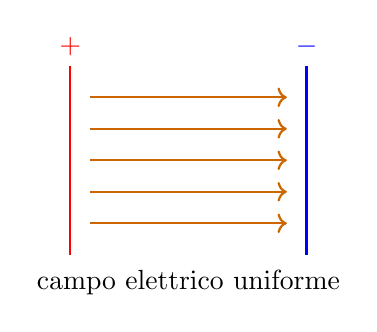
\begin{tikzpicture}[scale=1]
        \draw[thick,red] (0,-1.2) -- (0,1.2);
        \draw[thick,blue] (3.0,-1.2) -- (3.0,1.2);
        \node[red] at (0,1.45) {\(+\)};
        \node[blue] at (3.0,1.45) {\(-\)};
        \foreach \y in {-0.8,-0.4,0,0.4,0.8}{
            \draw[->,orange!80!black,thick] (0.25,\y) -- (2.75,\y);
        }
        \node at (1.5,-1.55) {campo elettrico uniforme};
    \end{tikzpicture}
\end{center}

Se la particella parte da ferma in \(x=0\), con velocità iniziale nulla, e il campo è diretto lungo \(x\), allora
\[
	x(t)=\frac{1}{2}at^2,
	\qquad
	v(t)=at,
	\qquad
	a=\frac{qE}{m}.
\]
Eliminando il tempo,
\[
	v^2=2ax=2\frac{qE}{m}x.
\]
Quindi
\[
	v(x)=\sqrt{\frac{2qEx}{m}}
\]
per una carica positiva accelerata nel verso del campo.

Lo stesso risultato si ottiene con il teorema dell'energia cinetica. Il lavoro del campo su una distanza \(x\) è
\[
	L=Fx=qEx.
\]
Poiché la particella parte da ferma,
\[
	\Delta K=\frac{1}{2}mv^2.
\]
Allora
\[
	qEx=\frac{1}{2}mv^2,
	\text{ da cui }
	v^2=\frac{2qEx}{m}.
\]

\begin{snippetexample}{Particella accelerata da un campo uniforme}
Se una particella di carica \(q>0\) e massa \(m\) parte da ferma in un campo uniforme \(E\), dopo aver percorso una distanza \(x\) nel verso del campo ha velocità
\[
	v(x)=\sqrt{\frac{2qEx}{m}}.
\]
\end{snippetexample}

Fuori dalla regione in cui il campo elettrico è presente, la forza elettrica si annulla. La particella prosegue allora con moto rettilineo uniforme, mantenendo la velocità raggiunta all'uscita.

\section{Esperimento di Millikan e quantizzazione della carica}

All'inizio del Novecento era ormai chiaro che nei fenomeni elettrici intervenivano particelle cariche molto piccole. Thomson aveva mostrato l'esistenza dell'elettrone, una particella carica negativamente con rapporto \(e/m\) costante. Millikan propose un esperimento per misurare direttamente la carica dell'elettrone e per verificare se la carica elettrica fosse continua oppure quantizzata.

\begin{snippetdefinition}{Quantizzazione della carica}
La carica elettrica è quantizzata se può assumere solo valori multipli interi di una carica elementare \(e\):
\[
	q=ne,
	\qquad
	n\in\naturalnumbers.
\]
\end{snippetdefinition}

Nell'esperimento di Millikan si osservano piccole gocce d'olio tra due piastre. Le gocce possono caricarsi elettricamente. Agiscono su di esse:
\begin{itemize}
	\item la forza peso \(\vec{F}_g=m\vec{g}\);
	\item la forza di attrito viscoso dell'aria, opposta al moto;
	\item la forza elettrica \(\vec{F}_e=q\vec{E}\), quando il campo elettrico è acceso.
\end{itemize}

Per piccole velocità, la forza di attrito viscoso è descritta dalla legge di Stokes:
\[
	F_a=6\pi\eta rv,
\]
dove \(\eta\) è la viscosità dell'aria, \(r\) è il raggio della goccia e \(v\) è la velocità.

\begin{center}
    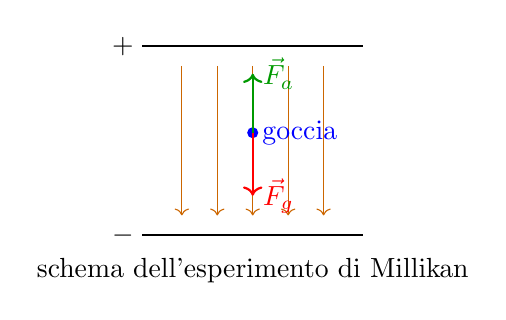
\begin{tikzpicture}[scale=1]
        \draw[thick] (-1.4,1.2) -- (1.4,1.2);
        \draw[thick] (-1.4,-1.2) -- (1.4,-1.2);
        \node at (-1.65,1.2) {\(+\)};
        \node at (-1.65,-1.2) {\(-\)};
        \foreach \x in {-0.9,-0.45,0,0.45,0.9}{
            \draw[->,orange!80!black] (\x,0.95) -- (\x,-0.95);
        }
        \fill[blue] (0,0.1) circle (2pt) node[right] {goccia};
        \draw[->,red,thick] (0,0.1) -- (0,-0.7) node[right] {\(\vec{F}_g\)};
        \draw[->,green!60!black,thick] (0,0.1) -- (0,0.85) node[right] {\(\vec{F}_a\)};
        \node at (0,-1.65) {schema dell'esperimento di Millikan};
    \end{tikzpicture}
\end{center}

\subsection{Caduta senza campo elettrico}

Quando il campo elettrico è spento, sulla goccia agiscono il peso e l'attrito viscoso. L'equazione del moto lungo la verticale è
\[
	ma=mg-6\pi\eta rv.
\]
Dopo un transitorio, la goccia raggiunge una velocità limite \(v_0\), per cui l'accelerazione è nulla:
\[
	0=mg-6\pi\eta rv_0.
\]
Quindi
\[
	v_0=\frac{mg}{6\pi\eta r}.
\]
Questa velocità limite può essere misurata sperimentalmente.

La massa della goccia si può scrivere in termini della densità \(\delta\) dell'olio:
\[
	m=\delta\frac{4}{3}\pi r^3.
\]
Sostituendo nella formula di \(v_0\), si ottiene
\[
	v_0=\frac{\frac{4}{3}\pi r^3\delta g}{6\pi\eta r}
	=\frac{2\delta g}{9\eta}r^2.
\]
Quindi, misurando \(v_0\), si può ricavare il raggio \(r\) della goccia:
\[
	r^2=\frac{9\eta v_0}{2\delta g}.
\]

\subsection{Moto con campo elettrico acceso}

Accendiamo ora il campo elettrico. Se la goccia ha carica \(q\), subisce la forza elettrica di modulo
\[
	F_e=qE.
\]
A seconda del segno della carica e del verso del campo, la forza elettrica può essere diretta verso l'alto o verso il basso. Nel caso in cui la forza elettrica sia verso l'alto, l'equazione alla velocità limite \(v_E\) diventa
\[
	0=mg-qE-6\pi\eta rv_E,
\]
con la convenzione dei segni scelta in modo coerente con il moto osservato. Da questa relazione si può isolare la carica:
\[
	qE=mg-6\pi\eta rv_E.
\]
Quindi
\[
	q=\frac{mg-6\pi\eta rv_E}{E}.
\]
La quantità a destra è misurabile, perché \(m\) e \(r\) sono stati ricavati dalla velocità limite senza campo, mentre \(v_E\) ed \(E\) si misurano durante l'esperimento.

In una forma equivalente, confrontando le velocità limite senza campo e con campo, si può scrivere
\[
	v_0=\frac{mg}{6\pi\eta r},
	\qquad
	v_E=v_0-\frac{qE}{6\pi\eta r}.
\]
Da cui
\[
	v_0-v_E=\frac{qE}{6\pi\eta r}.
\]
Pertanto
\[
	q=\frac{6\pi\eta r}{E}(v_0-v_E).
\]

\begin{snippettheorem}{Risultato dell'esperimento di Millikan}
Millikan trovò che le cariche misurate sulle gocce erano sempre multipli interi di una carica elementare:
\[
	q=ne,
	\qquad
	n=1,2,3,\dots
\]
con
\[
	e\simeq 1.6\cdot 10^{-19}\,\mathrm{C}.
\]
Questo mostra che la carica elettrica è quantizzata.
\end{snippettheorem}

Storicamente, l'esperimento di Millikan fu pubblicato nel 1910. Millikan ricevette il Premio Nobel per la Fisica nel 1923.

\section{Verso le distribuzioni continue di carica}

Il passo successivo è calcolare il campo elettrico prodotto da distribuzioni di carica non puntiformi, per esempio distribuzioni lineari, superficiali o volumiche. Se il punto di osservazione è
\[
	P=(x_P,y_P,z_P),
\]
vogliamo determinare
\[
	\vec{E}(P)=\vec{E}(x_P,y_P,z_P).
\]
Per farlo, si scompone la distribuzione in elementi infinitesimi di carica e si sommano i contributi tramite un integrale.


\pagebreak
\part{Lezione 3}

\section{Campo elettrico generato da una distribuzione di cariche}

La carica elettrica è quantizzata. La carica elementare ha modulo
\[
    q_e=1.6\cdot 10^{-19}\,\mathrm{C}.
\]
Però, nelle situazioni macroscopiche, il numero di cariche elementari coinvolte è enorme, spesso dell'ordine di \(10^{15}\)-\(10^{18}\) o anche maggiore. Per questo motivo, quando osserviamo una distribuzione di carica da distanze molto più grandi della scala atomica,
\[
    \text{distanza di osservazione}\gg 10^{-10}\,\mathrm{m},
\]
la carica può essere trattata come una distribuzione continua.

\subsection{Campo generato da cariche puntiformi}

Consideriamo una carica puntiforme \(q_1\). Il campo elettrico nel punto \(P\) è
\[
    \vec{E}(P)=\frac{q_1}{4\pi\varepsilon_0r^2}\hat{u},
\]
dove \(r\) è la distanza tra la carica e il punto \(P\), mentre \(\hat{u}\) è il versore diretto dalla carica verso \(P\).

\begin{center}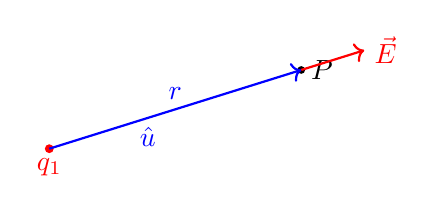
\begin{tikzpicture}[scale=1]
\fill[red] (0,0) circle (1.6pt) node[below] {\(q_1\)};
\fill (3.2,1.0) circle (1.4pt) node[right] {\(P\)};
\draw[->,blue,thick] (0,0) -- (3.2,1.0) node[midway,above] {\(r\)};
\draw[->,red,thick] (3.2,1.0) -- (4.0,1.25) node[right] {\(\vec{E}\)};
\node[blue] at (1.25,0.15) {\(\hat{u}\)};
\end{tikzpicture}\end{center}

Se sono presenti \(N\) cariche puntiformi \(q_1,\dots,q_N\), il campo totale si ottiene per sovrapposizione:
\[
    \vec{E}(P)=\sum_{i=1}^N\frac{q_i}{4\pi\varepsilon_0r_i^2}\hat{u}_i.
\]
Qui \(r_i\) è la distanza tra la carica \(q_i\) e il punto \(P\), mentre \(\hat{u}_i\) è il versore diretto da \(q_i\) verso \(P\).

\begin{snippetproposition}{Principio di sovrapposizione per il campo elettrico}
Il campo elettrico generato da più cariche puntiformi è la somma vettoriale dei campi generati dalle singole cariche:
\[
    \vec{E}(P)=\sum_{i=1}^N\vec{E}_i(P).
\]
\end{snippetproposition}

\section{Passaggio al continuo}

Quando le cariche sono moltissime e la distanza di osservazione è grande rispetto alla distanza tipica tra cariche elementari, possiamo sostituire la somma discreta con un integrale.

L'idea è la seguente:
\[
    q_i\longrightarrow dq,
\qquad
\sum_{i=1}^N\longrightarrow \int.
\]
Ogni elemento infinitesimo di carica \(dq\) produce un contributo
\[
    d\vec{E}=\frac{1}{4\pi\varepsilon_0}\frac{dq}{r^2}\hat{u},
\]
dove \(r\) è la distanza tra \(dq\) e il punto di osservazione.

Sommando tutti i contributi infinitesimi,
\[
    \vec{E}(P)=\frac{1}{4\pi\varepsilon_0}\int \frac{dq}{r^2}\hat{u}.
\]
L'integrale è vettoriale: bisogna sommare non solo i moduli, ma anche le direzioni dei contributi.

\begin{snippettheorem}{Campo elettrico di una distribuzione continua}
Il campo elettrico generato da una distribuzione continua di carica è
\[
    \vec{E}(P)=\frac{1}{4\pi\varepsilon_0}\int \frac{dq}{r^2}\hat{u},
\]
dove \(r\) è la distanza dall'elemento di carica \(dq\) al punto \(P\), e \(\hat{u}\) è il versore diretto da \(dq\) verso \(P\).
\end{snippettheorem}

\begin{center}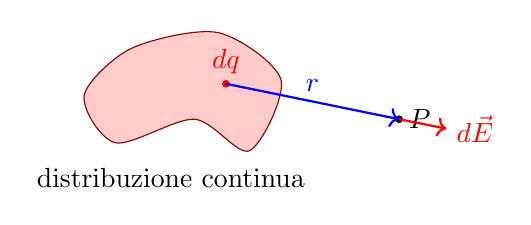
\begin{tikzpicture}[scale=1]
\draw[fill=red!20,draw=red!50!black] plot[smooth cycle] coordinates {(0,0) (1.0,0.3) (1.7,-0.1) (2.1,0.8) (1.3,1.4) (0.2,1.2) (-0.4,0.6)};
\fill (3.6,0.3) circle (1.4pt) node[right] {\(P\)};
\fill[red] (1.4,0.75) circle (1.4pt) node[above] {\(dq\)};
\draw[->,blue,thick] (1.4,0.75) -- (3.6,0.3) node[midway,above] {\(r\)};
\draw[->,red,thick] (3.6,0.3) -- (4.2,0.18) node[right] {\(d\vec{E}\)};
\node at (0.7,-0.45) {distribuzione continua};
\end{tikzpicture}\end{center}

\section{Densità di carica}

Per descrivere distribuzioni continue si introducono densità di carica diverse a seconda della geometria della distribuzione.

\subsection{Distribuzione lineare di carica}

Se la carica è distribuita lungo una curva, si introduce la densità lineare di carica.

\begin{snippetdefinition}{Densità lineare di carica}
La densità lineare di carica è
\[
    \lambda=\frac{dq}{d\ell}.
\]
Quindi
\[
    dq=\lambda\,d\ell.
\]
La sua unità di misura è
\[
    [\lambda]=\frac{\mathrm{C}}{\mathrm{m}}.
\]
\end{snippetdefinition}

La carica totale contenuta in una curva \(L\) è
\[
    q=\int_L dq=\int_L \lambda\,d\ell.
\]
Se la distribuzione è uniforme, \(\lambda\) è costante e
\[
    q=\lambda L,
\qquad
\lambda=\frac{q}{L}.
\]

\begin{center}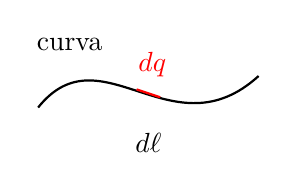
\begin{tikzpicture}[scale=1]
\draw[thick] (0,0) .. controls (0.8,1.0) and (1.7,-0.6) .. (2.8,0.4);
\draw[red,thick] (1.25,0.23) -- (1.55,0.13);
\node[red] at (1.45,0.55) {\(dq\)};
\node at (1.4,-0.45) {\(d\ell\)};
\node at (0.4,0.8) {curva};
\end{tikzpicture}\end{center}

\subsection{Distribuzione superficiale di carica}

Se la carica è distribuita su una superficie, si introduce la densità superficiale di carica.

\begin{snippetdefinition}{Densità superficiale di carica}
La densità superficiale di carica è
\[
    \sigma=\frac{dq}{d\Sigma}.
\]
Quindi
\[
    dq=\sigma\,d\Sigma.
\]
La sua unità di misura è
\[
    [\sigma]=\frac{\mathrm{C}}{\mathrm{m}^2}.
\]
\end{snippetdefinition}

La carica totale contenuta in una superficie \(\Sigma\) è
\[
    q=\int_\Sigma dq=\int_\Sigma \sigma\,d\Sigma.
\]
Se la distribuzione è uniforme, \(\sigma\) è costante e
\[
    q=\sigma\Sigma,
\qquad
\sigma=\frac{q}{\Sigma}.
\]

\begin{center}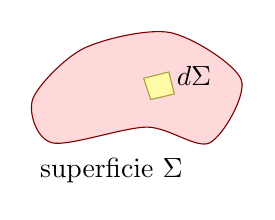
\begin{tikzpicture}[scale=1]
\draw[fill=red!15,draw=red!50!black] plot[smooth cycle] coordinates {(0,0) (1.2,0.2) (2.0,0.0) (2.4,0.8) (1.5,1.4) (0.4,1.2) (-0.25,0.55)};
\draw[fill=yellow!35,draw=yellow!60!black] (1.25,0.55) -- (1.55,0.62) -- (1.48,0.9) -- (1.16,0.82) -- cycle;
\node at (1.8,0.85) {\(d\Sigma\)};
\node at (0.75,-0.35) {superficie \(\Sigma\)};
\end{tikzpicture}\end{center}

\subsection{Distribuzione volumica di carica}

Se la carica è distribuita in un volume, si introduce la densità volumica di carica.

\begin{snippetdefinition}{Densità volumica di carica}
La densità volumica di carica è
\[
    \rho=\frac{dq}{dV}.
\]
Quindi
\[
    dq=\rho\,dV.
\]
La sua unità di misura è
\[
    [\rho]=\frac{\mathrm{C}}{\mathrm{m}^3}.
\]
\end{snippetdefinition}

La carica totale contenuta in un volume \(V\) è
\[
    q=\int_V dq=\int_V \rho\,dV.
\]
Se la distribuzione è uniforme, \(\rho\) è costante e
\[
    q=\rho V,
\qquad
\rho=\frac{q}{V}.
\]

\begin{center}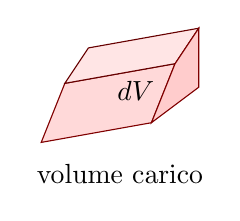
\begin{tikzpicture}[scale=1]
\draw[fill=red!15,draw=red!50!black] (0,0) -- (1.4,0.25) -- (1.7,1.0) -- (0.3,0.75) -- cycle;
\draw[fill=red!10,draw=red!40!black] (0.3,0.75) -- (1.7,1.0) -- (2.0,1.45) -- (0.6,1.2) -- cycle;
\draw[fill=red!20,draw=red!50!black] (1.4,0.25) -- (2.0,0.7) -- (2.0,1.45) -- (1.7,1.0) -- cycle;
\node at (1.2,0.65) {\(dV\)};
\node at (1.0,-0.4) {volume carico};
\end{tikzpicture}\end{center}

\section{Formula del campo per le tre distribuzioni}

Sostituendo l'espressione di \(dq\) nella formula generale del campo elettrico, si ottengono tre casi.

Per una distribuzione lineare:
\[
    \vec{E}(P)=\frac{1}{4\pi\varepsilon_0}\int_L\frac{\lambda\,d\ell}{r^2}\hat{u}.
\]
Per una distribuzione superficiale:
\[
    \vec{E}(P)=\frac{1}{4\pi\varepsilon_0}\int_\Sigma\frac{\sigma\,d\Sigma}{r^2}\hat{u}.
\]
Per una distribuzione volumica:
\[
    \vec{E}(P)=\frac{1}{4\pi\varepsilon_0}\int_V\frac{\rho\,dV}{r^2}\hat{u}.
\]

\begin{snippetproposition}{Campo elettrico da densità di carica}
La formula
\[
    \vec{E}(P)=\frac{1}{4\pi\varepsilon_0}\int\frac{dq}{r^2}\hat{u}
\]
si specializza in integrali di linea, superficie o volume a seconda che la distribuzione sia lineare, superficiale o volumica.
\end{snippetproposition}

\section{Esempio: anello uniformemente carico}

Consideriamo un anello di raggio \(R\), uniformemente carico con carica totale \(q\). Vogliamo calcolare il campo elettrico in un punto \(P\) sull'asse dell'anello, a distanza \(x\) dal centro.

\begin{center}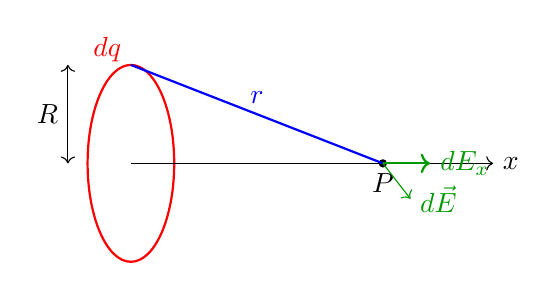
\begin{tikzpicture}[scale=1]
\draw[red,thick] (0,0) ellipse (0.55 and 1.25);
\draw[->] (0,0) -- (4.6,0) node[right] {\(x\)};
\fill (3.2,0) circle (1.5pt) node[below] {\(P\)};
\draw[blue,thick] (0,1.25) -- (3.2,0) node[midway,above] {\(r\)};
\draw[<->] (-0.8,0) -- (-0.8,1.25) node[midway,left] {\(R\)};
\draw[->,green!60!black,thick] (3.2,0) -- (3.8,0) node[right] {\(dE_x\)};
\draw[->,green!60!black] (3.2,0) -- (3.55,-0.45) node[right] {\(d\vec{E}\)};
\node[red] at (-0.3,1.45) {\(dq\)};
\end{tikzpicture}\end{center}

Per simmetria, i contributi trasversali di due elementi opposti dell'anello si cancellano. Rimane solo la componente lungo l'asse \(x\). Quindi il campo totale ha la forma
\[
    \vec{E}=E(x)\hat{x}.
\]

La densità lineare è
\[
    \lambda=\frac{q}{2\pi R},
\qquad
dq=\lambda\,d\ell.
\]
Ogni elemento dell'anello si trova alla stessa distanza dal punto \(P\):
\[
    r=\sqrt{R^2+x^2}.
\]
Se \(\theta\) è l'angolo tra \(d\vec{E}\) e l'asse \(x\), allora
\[
    \cos\theta=\frac{x}{r}=\frac{x}{\sqrt{R^2+x^2}}.
\]
La componente assiale del contributo infinitesimo è
\[
    dE_x=dE\cos\theta
=\frac{1}{4\pi\varepsilon_0}\frac{dq}{r^2}\cos\theta.
\]
Sostituendo:
\[
    dE_x=\frac{1}{4\pi\varepsilon_0}\frac{dq}{R^2+x^2}\frac{x}{\sqrt{R^2+x^2}}.
\]
Quindi
\begin{align*}
E(x)
&=\int_{\text{anello}}dE_x \\
&=\frac{1}{4\pi\varepsilon_0}\frac{x}{(R^2+x^2)^{3/2}}\int_{\text{anello}}dq \\
&=\frac{q}{4\pi\varepsilon_0}\frac{x}{(R^2+x^2)^{3/2}}.
\end{align*}

\begin{snippettheorem}{Campo sull'asse di un anello carico}
Il campo elettrico generato sull'asse di un anello uniformemente carico è
\[
    \vec{E}(x)=\frac{q}{4\pi\varepsilon_0}\frac{x}{(R^2+x^2)^{3/2}}\hat{x}.
\]
Il campo è nullo nel centro dell'anello, cioè per \(x=0\).
\end{snippettheorem}

\subsection{Limiti e massimo del campo}

Se \(x\gg R\), allora
\[
    (R^2+x^2)^{3/2}\simeq x^3,
\]
e quindi
\[
    E(x)\simeq \frac{q}{4\pi\varepsilon_0x^2}.
\]
A grandi distanze l'anello si comporta come una carica puntiforme \(q\).

Se \(|x|\ll R\), allora
\[
    (R^2+x^2)^{3/2}\simeq R^3,
\]
e quindi
\[
    E(x)\simeq \frac{q}{4\pi\varepsilon_0R^3}x.
\]
Vicino al centro, il campo cresce linearmente con \(x\).

Per trovare i punti in cui il modulo del campo è massimo, per \(x>0\) deriviamo
\[
    E(x)=\frac{q}{4\pi\varepsilon_0}x(R^2+x^2)^{-3/2}.
\]
Allora
\begin{align*}
\frac{dE}{dx}
&=\frac{q}{4\pi\varepsilon_0}\left[(R^2+x^2)^{-3/2}-3x^2(R^2+x^2)^{-5/2}\right] \\
&=\frac{q}{4\pi\varepsilon_0}\frac{R^2-2x^2}{(R^2+x^2)^{5/2}}.
\end{align*}
Il massimo positivo si ha quando
\[
    R^2-2x^2=0,
\qquad
x=\frac{R}{\sqrt{2}}.
\]
Per simmetria, il minimo negativo si trova in
\[
    x=-\frac{R}{\sqrt{2}}.
\]

\begin{center}\begin{tikzpicture}[scale=1]
\draw[->] (-3.2,0) -- (3.2,0) node[right] {\(x\)};
\draw[->] (0,-1.5) -- (0,1.7) node[above] {\(E(x)\)};
\draw[blue,thick,domain=-3:3,samples=200] plot (\x,{1.8*\x/(1+\x*\x)^(1.5)});
\draw[dashed] (0.707,0) -- (0.707,0.68);
\draw[dashed] (-0.707,0) -- (-0.707,-0.68);
\node[below] at (0.707,0) {\(\frac{R}{\sqrt{2}}\)};
\node[above] at (-0.85,0) {\(-\frac{R}{\sqrt{2}}\)};
\end{tikzpicture}\end{center}

\section{Esempio: disco uniformemente carico}

Consideriamo un disco di raggio \(R\), uniformemente carico con carica totale \(q\). La densità superficiale di carica è
\[
    \sigma=\frac{q}{\pi R^2}.
\]
Vogliamo calcolare il campo elettrico in un punto \(P\) sull'asse del disco, a distanza \(x\) dal centro.

L'idea è scomporre il disco in anelli concentrici di raggio \(r\) e spessore \(dr\). L'area di un anello infinitesimo è
\begin{align*}
d\Sigma
&=\pi(r+dr)^2-\pi r^2 \\
&=\pi(r^2+2r\,dr+dr^2)-\pi r^2 \\
&\simeq 2\pi r\,dr,
\end{align*}
poiché \(dr^2\) è trascurabile. Quindi la carica dell'anello 
\[
    dq=\sigma\,d\Sigma=\sigma\,2\pi r\,dr.
\]

\begin{center}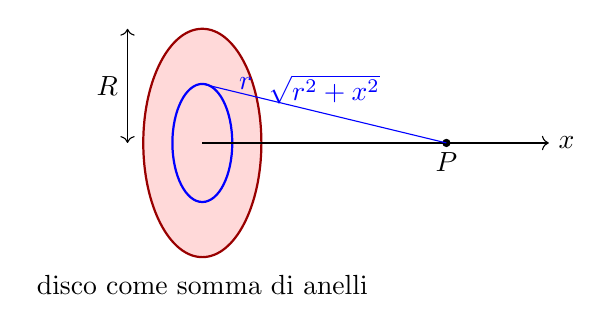
\begin{tikzpicture}[scale=1]
\draw[fill=red!15,draw=red!60!black,thick] (0,0) ellipse (0.75 and 1.45);
\draw[blue,thick] (0,0) ellipse (0.38 and 0.75);
\draw[->] (0,0) -- (4.4,0) node[right] {\(x\)};
\fill (3.1,0) circle (1.5pt) node[below] {\(P\)};
\draw[blue] (0,0.75) -- (3.1,0) node[midway,above] {\(\sqrt{r^2+x^2}\)};
\draw[<->] (-0.95,0) -- (-0.95,1.45) node[midway,left] {\(R\)};
\node[blue] at (0.55,0.75) {\(r\)};
\node at (0,-1.8) {disco come somma di anelli};
\end{tikzpicture}\end{center}

Usiamo il risultato trovato per l'anello, sostituendo \(R\) con \(r\) e \(q\) con \(dq\). Il contributo al campo lungo l'asse è
\[
    dE_x=\frac{dq}{4\pi\varepsilon_0}\frac{x}{(r^2+x^2)^{3/2}}.
\]
Sostituendo \(dq=\sigma2\pi r\,dr\), otteniamo
\[
    dE_x=\frac{\sigma x}{2\varepsilon_0}\frac{r\,dr}{(r^2+x^2)^{3/2}}.
\]
Il campo totale è quindi
\begin{align*}
E_x(x)
&=\frac{\sigma x}{2\varepsilon_0}\integral[0][R][\frac{r}{(r^2+x^2)^{3/2}}][r].
\end{align*}

Calcoliamo l'integrale con il cambio di variabile
\[
    y=r^2+x^2,
\qquad
dy=2r\,dr.
\]
Allora
\begin{align*}
\integral[\frac{r}{(r^2+x^2)^{3/2}}][r]
&=\frac{1}{2}\integral[y^{-3/2}][y] \\
&=-\frac{1}{\sqrt{y}} \\
&=-\frac{1}{\sqrt{r^2+x^2}}.
\end{align*}
Quindi
\begin{align*}
E_x(x)
&=\frac{\sigma x}{2\varepsilon_0}\left[-\frac{1}{\sqrt{r^2+x^2}}\right]_0^R \\
&=\frac{\sigma x}{2\varepsilon_0}\left(\frac{1}{|x|}-\frac{1}{\sqrt{R^2+x^2}}\right).
\end{align*}
Poiché
\[
    \frac{x}{|x|}=\operatorname{sgn}(x),
\]
possiamo scrivere
\[
    \vec{E}(x)=\frac{\sigma}{2\varepsilon_0}\left(\operatorname{sgn}(x)-\frac{x}{\sqrt{R^2+x^2}}\right)\hat{x}.
\]

Equivalentemente,
\[
    \vec{E}(x)=\frac{\sigma}{2\varepsilon_0}\left(\pm 1-\frac{x}{\sqrt{R^2+x^2}}\right)\hat{x},
\]
dove il segno \(+\) vale per \(x>0\), mentre il segno \(-\) vale per \(x<0\).

\begin{snippettheorem}{Campo sull'asse di un disco carico}
Il campo elettrico sull'asse di un disco uniformemente carico è
\[
    \vec{E}(x)=\frac{\sigma}{2\varepsilon_0}\left(\operatorname{sgn}(x)-\frac{x}{\sqrt{R^2+x^2}}\right)\hat{x}.
\]
Per \(x>0\):
\[
    \vec{E}(x)=\frac{\sigma}{2\varepsilon_0}\left(1-\frac{x}{\sqrt{R^2+x^2}}\right)\hat{x}.
\]
Per \(x<0\):
\[
    \vec{E}(x)=\frac{\sigma}{2\varepsilon_0}\left(-1-\frac{x}{\sqrt{R^2+x^2}}\right)\hat{x}.
\]
\end{snippettheorem}

\subsection{Limiti del campo del disco}

Per \(|x|\ll R\), il termine
\[
    \frac{x}{\sqrt{R^2+x^2}}
\]
è trascurabile rispetto a \(1\). Quindi
\[
    \vec{E}(0^+)=\frac{\sigma}{2\varepsilon_0}\hat{x},
\qquad
\vec{E}(0^-)=-\frac{\sigma}{2\varepsilon_0}\hat{x}.
\]
Il campo ha una discontinuità attraversando il disco carico:
\[
    \Delta E=\frac{\sigma}{\varepsilon_0}.
\]

Per \(|x|\gg R\), consideriamo \(x>0\). Allora
\[
    \frac{x}{\sqrt{R^2+x^2}}
=\frac{1}{\sqrt{1+\frac{R^2}{x^2}}}
\simeq 1-\frac{R^2}{2x^2}.
\]
Quindi
\[
    E_x(x)\simeq\frac{\sigma}{2\varepsilon_0}\left(1-1+\frac{R^2}{2x^2}\right)
=\frac{\sigma R^2}{4\varepsilon_0x^2}.
\]
Poiché \(q=\sigma\pi R^2\), otteniamo
\[
    E_x(x)\simeq\frac{q}{4\pi\varepsilon_0x^2}.
\]
Dunque, a grandi distanze, il disco si comporta come una carica puntiforme.

\begin{center}\begin{tikzpicture}[scale=1]
\draw[->] (-3.3,0) -- (3.3,0) node[right] {\(x\)};
\draw[->] (0,-1.6) -- (0,1.8) node[above] {\(E_x\)};
\draw[blue,thick,domain=0.08:3.0,samples=160] plot (\x,{1.2*(1-\x/sqrt(1+\x*\x))});
\draw[blue,thick,domain=-3.0:-0.08,samples=160] plot (\x,{1.2*(-1-\x/sqrt(1+\x*\x))});
\draw[red,thick] (0,-1.2) -- (0,1.2);
\node[left] at (0,1.2) {\(\frac{\sigma}{2\varepsilon_0}\)};
\node[right] at (0,-1.2) {\(-\frac{\sigma}{2\varepsilon_0}\)};
\node at (2.0,0.45) {\(\to0\)};
\node at (-2.0,-0.45) {\(\to0\)};
\end{tikzpicture}\end{center}


\pagebreak
\part{Lezione 4}

\section{Campo sull'asse di un disco uniformemente carico}

Consideriamo un disco di raggio \(R\), uniformemente carico con densità superficiale \(\sigma\). Sull'asse del disco, scegliendo l'origine nel centro e l'asse \(x\) perpendicolare al disco, il campo elettrico ha solo componente lungo \(x\).

Dalla lezione precedente abbiamo ottenuto il potenziale
\[
    V(x)=\frac{\sigma}{2\varepsilon_0}\left(\sqrt{R^2+x^2}-|x|\right).
\]
Il campo elettrico si ricava derivando il potenziale:
\[
    E_x(x)=-\frac{dV}{dx}.
\]
Poiché
\[
    \frac{d}{dx}|x|=\operatorname{sgn}(x)
=
\begin{cases}
1, & x>0,\\
-1, & x<0,
\end{cases}
\]
si ha, per \(x\neq0\),
\begin{align*}
E_x(x)
&=-\frac{d}{dx}\left[\frac{\sigma}{2\varepsilon_0}\left(\sqrt{R^2+x^2}-|x|\right)\right] \\
&=\frac{\sigma}{2\varepsilon_0}\left(\operatorname{sgn}(x)-\frac{x}{\sqrt{R^2+x^2}}\right).
\end{align*}
Equivalentemente,
\[
    \vec{E}(x)=\frac{\sigma}{2\varepsilon_0}\left(1-\frac{|x|}{\sqrt{R^2+x^2}}\right)\operatorname{sgn}(x)\hat{x}.
\]

In forma separata:
\[
    \vec{E}(x)=
\begin{cases}
\displaystyle \frac{\sigma}{2\varepsilon_0}\left(1-\frac{x}{\sqrt{R^2+x^2}}\right)\hat{x}, & x>0,\\[8pt]
\displaystyle -\frac{\sigma}{2\varepsilon_0}\left(1+\frac{x}{\sqrt{R^2+x^2}}\right)\hat{x}, & x<0.
\end{cases}
\]

\begin{center}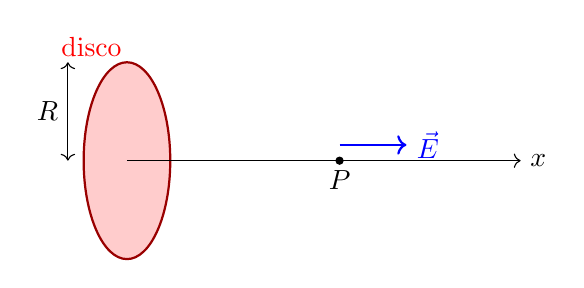
\begin{tikzpicture}[scale=1]
\draw[fill=red!20,draw=red!60!black,thick] (0,0) ellipse (0.55 and 1.25);
\draw[->] (0,0) -- (5,0) node[right] {\(x\)};
\node[red] at (-0.45,1.45) {disco};
\draw[<->] (-0.75,0) -- (-0.75,1.25) node[midway,left] {\(R\)};
\fill (2.7,0) circle (1.5pt) node[below] {\(P\)};
\draw[->,blue,thick] (2.7,0.2) -- (3.55,0.2) node[right] {\(\vec{E}\)};
\end{tikzpicture}\end{center}

\subsection{Limiti notevoli}

Se il punto è molto vicino al centro del disco rispetto al raggio, cioè
\[
    |x|\ll R,
\]
allora
\[
    \frac{|x|}{\sqrt{R^2+x^2}}\simeq0.
\]
Quindi
\[
    \vec{E}(x)\simeq
\begin{cases}
\displaystyle \frac{\sigma}{2\varepsilon_0}\hat{x}, & x>0,\\[6pt]
\displaystyle -\frac{\sigma}{2\varepsilon_0}\hat{x}, & x<0.
\end{cases}
\]

Se invece il punto è molto lontano dal disco, cioè
\[
    |x|\gg R,
\]
il disco si comporta come una carica puntiforme di carica totale
\[
    q=\sigma\pi R^2.
\]
Infatti, per \(x>0\),
\[
    1-\frac{x}{\sqrt{x^2+R^2}}\simeq \frac{R^2}{2x^2},
\]
e dunque
\[
    E_x(x)\simeq \frac{\sigma R^2}{4\varepsilon_0x^2}
=\frac{q}{4\pi\varepsilon_0x^2}.
\]

\begin{snippetproposition}{Campo del disco sull'asse}
Il campo elettrico sull'asse di un disco uniformemente carico è
\[
    \vec{E}(x)=\frac{\sigma}{2\varepsilon_0}\left(1-\frac{|x|}{\sqrt{R^2+x^2}}\right)\operatorname{sgn}(x)\hat{x}.
\]
Vicino al centro di un disco molto grande il campo è quasi costante; molto lontano il disco si comporta come una carica puntiforme.
\end{snippetproposition}

\section{Piano infinito uniformemente carico}

Un piano infinito uniformemente carico si può ottenere come limite di un disco di raggio \(R\) quando
\[
    R\to\infty,
\]
mantenendo costante la densità superficiale \(\sigma\). In questo limite, per ogni punto a distanza finita dal piano,
\[
    \frac{|x|}{\sqrt{R^2+x^2}}\to0.
\]
Pertanto
\[
    \vec{E}(x)=
\begin{cases}
\displaystyle \frac{\sigma}{2\varepsilon_0}\hat{x}, & x>0,\\[6pt]
\displaystyle -\frac{\sigma}{2\varepsilon_0}\hat{x}, & x<0.
\end{cases}
\]

\begin{snippettheorem}{Campo di un piano infinito uniformemente carico}
Un piano infinito con densità superficiale di carica \(\sigma\) genera un campo elettrico uniforme su ciascun lato del piano, perpendicolare al piano:
\[
    E=\frac{\sigma}{2\varepsilon_0}.
\]
Se \(\sigma>0\), il campo è uscente dal piano; se \(\sigma<0\), il campo è entrante nel piano.
\end{snippettheorem}

\begin{center}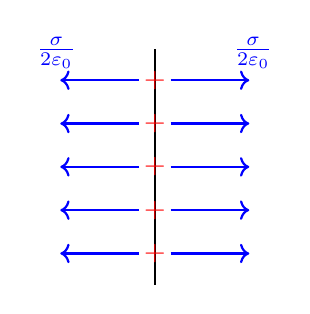
\begin{tikzpicture}[scale=1]
\draw[thick] (0,-1.5) -- (0,1.5);
\foreach \y in {-1.1,-0.55,0,0.55,1.1}{
\node[red] at (0,\y) {\(+\)};
\draw[->,blue,thick] (0.2,\y) -- (1.2,\y);
\draw[->,blue,thick] (-0.2,\y) -- (-1.2,\y);
}
\node[blue] at (1.25,1.45) {\(\frac{\sigma}{2\varepsilon_0}\)};
\node[blue] at (-1.25,1.45) {\(\frac{\sigma}{2\varepsilon_0}\)};
\end{tikzpicture}\end{center}

Il campo elettrico ha una discontinuità attraversando il piano. Il salto della componente normale è
\[
    \Delta E=\frac{\sigma}{\varepsilon_0}.
\]
Infatti appena a destra il campo vale \(\sigma/(2\varepsilon_0)\hat{x}\), mentre appena a sinistra vale \(-\sigma/(2\varepsilon_0)\hat{x}\).

\begin{center}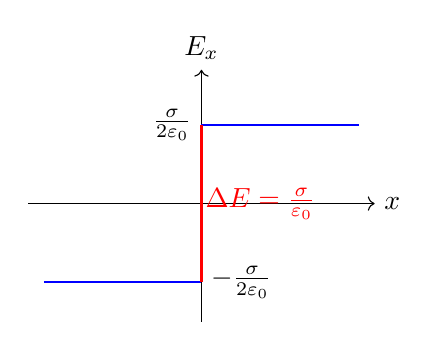
\begin{tikzpicture}[scale=1]
\draw[->] (-2.2,0) -- (2.2,0) node[right] {\(x\)};
\draw[->] (0,-1.5) -- (0,1.7) node[above] {\(E_x\)};
\draw[blue,thick] (-2,-1) -- (0,-1);
\draw[blue,thick] (0,1) -- (2,1);
\draw[red,thick] (0,-1) -- (0,1);
\node[left] at (0,1) {\(\frac{\sigma}{2\varepsilon_0}\)};
\node[right] at (0,-1) {\(-\frac{\sigma}{2\varepsilon_0}\)};
\node[red] at (0.75,0) {\(\Delta E=\frac{\sigma}{\varepsilon_0}\)};
\end{tikzpicture}\end{center}

\section{Condensatore piano ideale}

Consideriamo due piani infiniti paralleli, carichi con densità superficiali opposte:
\[
    +\sigma,
\qquad
-\sigma.
\]
Questo è il modello ideale di un condensatore piano, lontano dai bordi.

\begin{center}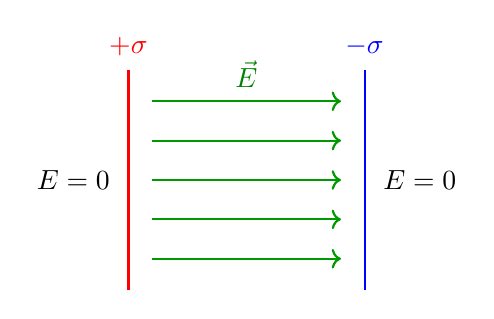
\begin{tikzpicture}[scale=1]
\draw[thick,red] (0,-1.4) -- (0,1.4);
\draw[thick,blue] (3,-1.4) -- (3,1.4);
\node[red] at (0,1.7) {\(+\sigma\)};
\node[blue] at (3,1.7) {\(-\sigma\)};
\foreach \y in {-1.0,-0.5,0,0.5,1.0}{
\draw[->,green!60!black,thick] (0.3,\y) -- (2.7,\y);
}
\node[green!50!black] at (1.5,1.35) {\(\vec{E}\)};
\node at (-0.7,0) {\(E=0\)};
\node at (3.7,0) {\(E=0\)};
\end{tikzpicture}\end{center}

Il campo prodotto dal piano positivo è uscente da esso, mentre il campo prodotto dal piano negativo è entrante verso di esso. Per sovrapposizione:
\begin{itemize}
\item all'esterno del condensatore i due campi hanno verso opposto e si cancellano;
\item all'interno del condensatore i due campi hanno lo stesso verso e si sommano.
\end{itemize}
Dunque
\[
    E_{\mathrm{interno}}=\frac{\sigma}{2\varepsilon_0}+\frac{\sigma}{2\varepsilon_0}=\frac{\sigma}{\varepsilon_0},
\]
mentre
\[
    E_{\mathrm{esterno}}=0.
\]

\begin{snippetproposition}{Campo del condensatore piano ideale}
Tra due piani infiniti paralleli con densità di carica \(+\sigma\) e \(-\sigma\), il campo elettrico è uniforme e vale
\[
    E=\frac{\sigma}{\varepsilon_0}.
\]
All'esterno dei due piani il campo è nullo.
\end{snippetproposition}

\section{Lavoro elettrico e potenziale elettrostatico}

Passiamo ora al lavoro compiuto dal campo elettrico e alla definizione di potenziale elettrostatico.

Se una carica \(q\) è immersa in un campo elettrico \(\vec{E}\), la forza elettrica agente su di essa è
\[
    \vec{F}_e=q\vec{E}.
\]
Equivalentemente,
\[
    \vec{E}=\frac{\vec{F}_e}{q}.
\]

\begin{snippetdefinition}{Forza conservativa}
Una forza \(\vec{F}\) si dice conservativa se il lavoro compiuto da \(A\) a \(B\) dipende solo dai punti iniziale e finale, non dal percorso seguito:
\[
    \int_{\gamma_1} \vec{F}\cdot d\vec{s}
    =
    \int_{\gamma_2} \vec{F}\cdot d\vec{s}
    \qquad\text{per qualunque coppia di cammini \(\gamma_1,\gamma_2\) da \(A\) a \(B\)}.
\]
Equivalentemente, la circuitazione lungo ogni curva chiusa è nulla:
\[
    \oint \vec{F}\cdot d\vec{s}=0.
\]
\end{snippetdefinition}

In elettrostatica il campo elettrico è generato da cariche ferme. In questo caso la forza elettrica è conservativa. Se invece i campi dipendono dal tempo, come avviene in elettrodinamica, il campo elettrico può non essere conservativo.

\begin{snippetproposition}{Conservatività del campo elettrostatico}
In elettrostatica la forza elettrica è conservativa. Di conseguenza anche il campo elettrico è conservativo:
\[
    \oint \vec{E}\cdot d\vec{s}=0.
\]
\end{snippetproposition}

\begin{center}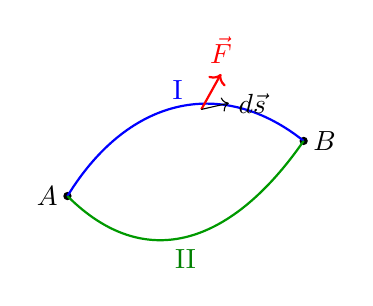
\begin{tikzpicture}[scale=1]
\fill (0,0) circle (1.5pt) node[left] {\(A\)};
\fill (3,0.7) circle (1.5pt) node[right] {\(B\)};
\draw[blue,thick] (0,0) .. controls (0.8,1.3) and (2.0,1.5) .. (3,0.7);
\draw[green!60!black,thick] (0,0) .. controls (1.0,-1.0) and (2.1,-0.6) .. (3,0.7);
\node[blue] at (1.4,1.35) {I};
\node[green!50!black] at (1.5,-0.8) {II};
\draw[->,red,thick] (1.7,1.1) -- (1.95,1.55) node[above] {\(\vec{F}\)};
\draw[->,black] (1.7,1.1) -- (2.05,1.18) node[right] {\(d\vec{s}\)};
\end{tikzpicture}\end{center}

Se una forza è conservativa, esiste una funzione scalare, detta energia potenziale, tale che
\[
    W_{A\to B}=\int_A^B \vec{F}\cdot d\vec{s}=U(A)-U(B).
\]
Nel caso elettrico, l'energia potenziale si indica con \(U_e\), quindi
\[
    \int_A^B \vec{F}_e\cdot d\vec{s}=U_e(A)-U_e(B).
\]
Sostituendo \(\vec{F}_e=q\vec{E}\):
\[
    q\int_A^B \vec{E}\cdot d\vec{s}=U_e(A)-U_e(B).
\]
Dividendo per \(q\), otteniamo
\[
    \int_A^B \vec{E}\cdot d\vec{s}=\frac{U_e(A)}{q}-\frac{U_e(B)}{q}.
\]

\begin{snippetdefinition}{Potenziale elettrostatico}
Il potenziale elettrostatico è l'energia potenziale elettrica per unità di carica:
\[
    V=\frac{U_e}{q}.
\]
La differenza di potenziale tra due punti 
\[
    V(A)-V(B)=\int_A^B \vec{E}\cdot d\vec{s}.
\]
\end{snippetdefinition}

Questa formula mostra che il potenziale diminuisce nel verso del campo elettrico. Infatti, se ci muoviamo lungo una linea di campo, allora \(d\vec{s}\) è parallelo a \(\vec{E}\) e
\[
    \vec{E}\cdot d\vec{s}=E\,ds.
\]
Inoltre localmente
\[
    E=-\frac{dV}{ds}.
\]
Infatti
\[
    \int_A^B E\,ds=\int_A^B -\frac{dV}{ds}\,ds
=-\int_A^B dV
=V(A)-V(B).
\]

\subsection{Unità di misura}

Poiché
\[
    V=\frac{U_e}{q},
\]
la sua unità di misura 
\[
    [V]=\frac{\mathrm{J}}{\mathrm{C}}=\mathrm{volt}=\mathrm{V}.
\]
Inoltre, dal legame \(E=-dV/ds\), si ottiene
\[
    [E]=\frac{\mathrm{V}}{\mathrm{m}}.
\]
Questa unità  equivalente a
\[
    [E]=\frac{\mathrm{N}}{\mathrm{C}}.
\]

\section{Potenziale di una carica puntiforme}

Consideriamo una carica puntiforme \(q\). Il campo elettrico è
\[
    \vec{E}(r)=\frac{q}{4\pi\varepsilon_0r^2}\hat{r}.
\]
Vogliamo calcolare la differenza di potenziale tra due punti \(A\) e \(B\), posti a distanze \(r_A\) e \(r_B\) dalla carica.

\begin{center}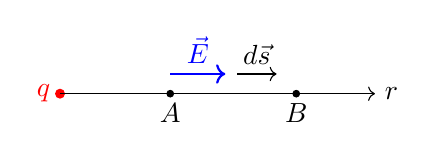
\begin{tikzpicture}[scale=1]
\fill[red] (0,0) circle (1.8pt) node[left] {\(q\)};
\draw[->] (0,0) -- (4,0) node[right] {\(r\)};
\fill (1.4,0) circle (1.4pt) node[below] {\(A\)};
\fill (3.0,0) circle (1.4pt) node[below] {\(B\)};
\draw[->,blue,thick] (1.4,0.25) -- (2.1,0.25) node[midway,above] {\(\vec{E}\)};
\draw[->,black] (2.25,0.25) -- (2.75,0.25) node[midway,above] {\(d\vec{s}\)};
\end{tikzpicture}\end{center}

Sulla direzione radiale, \(\hat{r}\cdot d\vec{s}=dr\). Quindi
\begin{align*}
V(A)-V(B)
&=\int_A^B \vec{E}\cdot d\vec{s} \\
&=\int_{r_A}^{r_B}\frac{q}{4\pi\varepsilon_0r^2}\,dr \\
&=\frac{q}{4\pi\varepsilon_0}\left[-\frac{1}{r}\right]_{r_A}^{r_B} \\
&=\frac{q}{4\pi\varepsilon_0}\left(\frac{1}{r_A}-\frac{1}{r_B}\right).
\end{align*}

Se scegliamo come riferimento
\[
    V(\infty)=0,
\]
e poniamo \(r_A=r\), \(r_B\to\infty\), otteniamo
\[
    V(r)=\frac{q}{4\pi\varepsilon_0r}.
\]

\begin{snippettheorem}{Potenziale di una carica puntiforme}
Il potenziale elettrostatico generato da una carica puntiforme \(q\), scegliendo \(V(\infty)=0\), è
\[
    V(r)=\frac{q}{4\pi\varepsilon_0r}.
\]
\end{snippettheorem}

Verifichiamo che da questo potenziale si recupera il campo:
\begin{align*}
E_r
&=-\frac{dV}{dr} \\
&=-\frac{d}{dr}\left(\frac{q}{4\pi\varepsilon_0}r^{-1}\right) \\
&=\frac{q}{4\pi\varepsilon_0r^2}.
\end{align*}

\section{Energia potenziale di una distribuzione di cariche puntiformi}

Il potenziale di una carica puntiforme è
\[
    V(r)=\frac{q}{4\pi\varepsilon_0r}.
\]
Una carica \(q_0\) posta in un punto in cui il potenziale è \(V\) ha energia potenziale
\[
    U_e=q_0V.
\]

\subsection{Sistema di due cariche}

Consideriamo due cariche puntiformi \(q_1\) e \(q_2\), poste a distanza \(r\). Per costruire la configurazione partendo dalle cariche all'infinito possiamo procedere così.

Per prima cosa portiamo \(q_1\) dall'infinito alla posizione finale. Non essendoci ancora altre cariche, il lavoro richiesto è
\[
    W_1=0.
\]
Poi portiamo \(q_2\) dall'infinito fino a distanza \(r\) da \(q_1\). Il potenziale prodotto da \(q_1\) nel punto finale è
\[
    V_1=\frac{q_1}{4\pi\varepsilon_0r}.
\]
Il lavoro dell'agente esterno necessario a costruire la configurazione, lentamente e senza variazione di energia cinetica, è
\[
    W_2=q_2V_1=\frac{q_1q_2}{4\pi\varepsilon_0r}.
\]
Questa è l'energia potenziale elettrostatica del sistema di due cariche:
\[
    U_e=\frac{q_1q_2}{4\pi\varepsilon_0r}.
\]

\begin{snippetproposition}{Energia potenziale di due cariche}
L'energia potenziale elettrostatica di due cariche puntiformi \(q_1\) e \(q_2\), a distanza \(r\), è
\[
    U_e=\frac{q_1q_2}{4\pi\varepsilon_0r}.
\]
Se le cariche hanno lo stesso segno, l'energia è positiva; se hanno segno opposto, l'energia è negativa.
\end{snippetproposition}

\begin{center}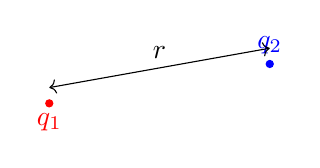
\begin{tikzpicture}[scale=1]
\fill[red] (0,0) circle (1.5pt) node[below] {\(q_1\)};
\fill[blue] (2.8,0.5) circle (1.5pt) node[above] {\(q_2\)};
\draw[<->] (0,0.2) -- (2.8,0.7) node[midway,above] {\(r\)};
\end{tikzpicture}\end{center}

\subsection{Sistema di tre cariche}

Aggiungiamo ora una terza carica \(q_3\). Quando \(q_1\) e \(q_2\) sono già state posizionate, il potenziale nel punto in cui portiamo \(q_3\) è la somma dei potenziali generati da \(q_1\) e \(q_2\):
\[
    V_{12}=\frac{q_1}{4\pi\varepsilon_0r_{13}}+\frac{q_2}{4\pi\varepsilon_0r_{23}}.
\]
Il lavoro per portare \(q_3\) dall'infinito è
\[
    W_3=q_3V_{12}
=q_3\left(\frac{q_1}{4\pi\varepsilon_0r_{13}}+\frac{q_2}{4\pi\varepsilon_0r_{23}}\right).
\]
Quindi l'energia totale del sistema è
\[
    U_e=\frac{q_1q_2}{4\pi\varepsilon_0r_{12}}
+\frac{q_1q_3}{4\pi\varepsilon_0r_{13}}
+\frac{q_2q_3}{4\pi\varepsilon_0r_{23}}.
\]

\begin{center}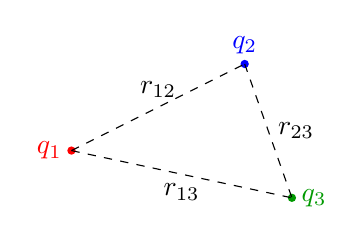
\begin{tikzpicture}[scale=1]
\fill[red] (0,0) circle (1.5pt) node[left] {\(q_1\)};
\fill[blue] (2.2,1.1) circle (1.5pt) node[above] {\(q_2\)};
\fill[green!60!black] (2.8,-0.6) circle (1.5pt) node[right] {\(q_3\)};
\draw[dashed] (0,0) -- (2.2,1.1) node[midway,above] {\(r_{12}\)};
\draw[dashed] (0,0) -- (2.8,-0.6) node[midway,below] {\(r_{13}\)};
\draw[dashed] (2.2,1.1) -- (2.8,-0.6) node[midway,right] {\(r_{23}\)};
\end{tikzpicture}\end{center}

\subsection{Sistema di \(N\) cariche}

Per \(N\) cariche puntiformi, l'energia potenziale elettrostatica totale si ottiene sommando il contributo di ogni coppia di cariche. Per evitare di contare due volte la stessa coppia, si inserisce un fattore \(1/2\).

\begin{snippettheorem}{Energia potenziale di \(N\) cariche puntiformi}
Per un sistema di \(N\) cariche puntiformi, l'energia potenziale elettrostatica è
\[
    U_e=\frac{1}{2}\sum_{\substack{i,j=1\\ i\neq j}}^N
\frac{q_iq_j}{4\pi\varepsilon_0r_{ij}}.
\]
Equivalentemente,
\[
    U_e=\sum_{i<j}\frac{q_iq_j}{4\pi\varepsilon_0r_{ij}}.
\]
\end{snippettheorem}

Questa energia è il lavoro che un agente esterno deve compiere per assemblare lentamente la configurazione partendo dalle cariche poste all'infinito.

\section{Potenziale in un campo elettrico uniforme}

Consideriamo un campo elettrico uniforme diretto lungo l'asse \(x\):
\[
    \vec{E}=E\hat{x}.
\]
Siano \(A\) e \(B\) due punti separati da una distanza \(d\) lungo il verso del campo. Allora
\[
    V(A)-V(B)=\int_A^B \vec{E}\cdot d\vec{s}=\int_A^B E\,dx=Ed.
\]
Quindi
\[
    E=\frac{V(A)-V(B)}{d}=-\frac{V(B)-V(A)}{d}.
\]

\begin{snippetproposition}{Differenza di potenziale in un campo uniforme}
In un campo elettrico uniforme, la differenza di potenziale tra due punti separati da una distanza \(d\) lungo la direzione del campo è
\[
    V(A)-V(B)=Ed.
\]
Il potenziale diminuisce nel verso del campo elettrico.
\end{snippetproposition}

\begin{center}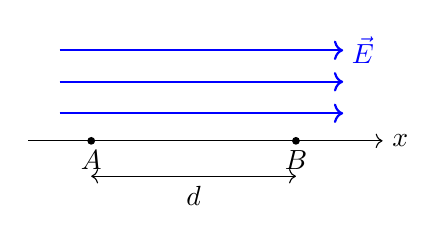
\begin{tikzpicture}[scale=1]
\draw[->] (0,0) -- (4.5,0) node[right] {\(x\)};
\fill (0.8,0) circle (1.4pt) node[below] {\(A\)};
\fill (3.4,0) circle (1.4pt) node[below] {\(B\)};
\draw[<->] (0.8,-0.45) -- (3.4,-0.45) node[midway,below] {\(d\)};
\foreach \y in {0.35,0.75,1.15}{
\draw[->,blue,thick] (0.4,\y) -- (4.0,\y);
}
\node[blue] at (4.25,1.15) {\(\vec{E}\)};
\end{tikzpicture}\end{center}

Nel condensatore piano ideale, se la distanza tra le armature è \(d\), si ha
\[
    E=\frac{V_+-V_-}{d}.
\]
Poich abbiamo trovato anche
\[
    E=\frac{\sigma}{\varepsilon_0},
\]
segue
\[
    V_+-V_-=\frac{\sigma d}{\varepsilon_0}.
\]

\section{Conduttori in equilibrio elettrostatico}

Un caso particolarmente importante è quello dei conduttori in equilibrio elettrostatico. In un conduttore all'equilibrio le cariche libere non si muovono. Se all'interno del conduttore esistesse un campo elettrico non nullo, le cariche subirebbero una forza e si muoverebbero. Dunque deve valere
\[
    \vec{E}=\vec{0}
\]
in ogni punto interno del conduttore.

Poiché
\[
    \vec{E}=\vec{0},
\]
allora il potenziale è costante in tutto il conduttore:
\[
    V=\text{costante}.
\]

\begin{snippettheorem}{Conduttore in equilibrio elettrostatico}
In un conduttore in equilibrio elettrostatico:
\begin{itemize}
\item il campo elettrico interno è nullo;
\item il potenziale è costante in tutto il conduttore e sulla sua superficie.
\end{itemize}
\end{snippettheorem}

\begin{center}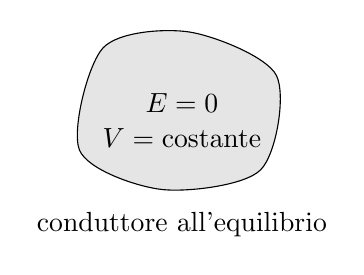
\begin{tikzpicture}[scale=1]
\draw[fill=gray!20,draw=black] plot[smooth cycle] coordinates {(-1.3,-0.5) (-1.0,0.8) (0.1,1.0) (1.2,0.45) (1.0,-0.75) (-0.25,-1.0)};
\node at (0,0.1) {\(E=0\)};
\node at (0,-0.35) {\(V=\text{costante}\)};
\node at (0,-1.45) {conduttore all'equilibrio};
\end{tikzpicture}\end{center}

\pagebreak
\part{Lezione 5}

\section{Lavoro di una forza e forze conservative}

Sia \(\vec{F}\) una forza che agisce su un punto materiale. Il lavoro compiuto dalla forza lungo un cammino orientato da \(A\) a \(B\) è
\[
    W_{A\to B}=\int_A^B \vec{F}\cdot d\vec{s}.
\]
In generale il lavoro può dipendere dal cammino seguito. Esiste però una classe importante di forze per cui il lavoro dipende solo dagli estremi.

\begin{snippetdefinition}{Forza conservativa}
Una forza \(\vec{F}\) si dice conservativa se il lavoro compiuto lungo un cammino da \(A\) a \(B\) dipende solo dagli estremi e non dal percorso scelto.
In tal caso esiste un'energia potenziale \(U\) tale che
\[
    W_{A\to B}=U(A)-U(B).
\]
\end{snippetdefinition}

Se una forza è conservativa, il lavoro lungo un percorso chiuso è nullo:
\[
    \oint \vec{F}\cdot d\vec{s}=0.
\]
Infatti, lungo un percorso chiuso il punto iniziale e il punto finale coincidono, quindi la variazione di energia potenziale è nulla.

\section{Campo elettrico e potenziale elettrico}

In elettrostatica la forza elettrica su una carica \(q\) immersa in un campo elettrico \(\vec{E}\) è
\[
    \vec{F}_e=q\vec{E}.
\]
Il campo elettrostatico è conservativo, quindi la forza elettrica è conservativa. Pertanto
\[
    W_{A\to B}=\int_A^B \vec{F}_e\cdot d\vec{s}=U_e(A)-U_e(B).
\]
Sostituendo \(\vec{F}_e=q\vec{E}\), otteniamo
\[
    q\int_A^B \vec{E}\cdot d\vec{s}=U_e(A)-U_e(B).
\]
Dividendo per \(q\), si introduce il potenziale elettrico
\[
    V=\frac{U_e}{q}.
\]
Quindi
\[
    \int_A^B \vec{E}\cdot d\vec{s}=V(A)-V(B).
\]

\begin{snippetdefinition}{Potenziale elettrico}
Il potenziale elettrico \(V\) è l'energia potenziale elettrica per unità di carica:
\[
    V=\frac{U_e}{q}.
\]
La differenza di potenziale tra due punti è legata al campo elettrico da
\[
    V(A)-V(B)=\int_A^B \vec{E}\cdot d\vec{s}.
\]
\end{snippetdefinition}

Lungo una linea di campo, se \(s\) è la coordinata lungo la linea, si ha
\[
    E=-\frac{dV}{ds}.
\]
Questa relazione esprime il fatto che il campo elettrico punta nella direzione in cui il potenziale diminuisce più rapidamente.

Per una carica puntiforme \(q\), scegliendo \(V(\infty)=0\), il potenziale è
\[
    V(r)=\frac{q}{4\pi\varepsilon_0r}.
\]

\section{Potenziale generato da distribuzioni continue di carica}

Per una distribuzione continua di carica, possiamo scomporre la distribuzione in elementi infinitesimi \(dq\). Ogni elemento produce nel punto \(P\) un contributo infinitesimo di potenziale
\[
    dV(P)=\frac{1}{4\pi\varepsilon_0}\frac{dq}{r},
\]
dove \(r\) è la distanza tra l'elemento \(dq\) e il punto \(P\). Il potenziale totale si ottiene sommando, cio integrando, tutti i contributi:
\[
    V(P)=\frac{1}{4\pi\varepsilon_0}\int \frac{dq}{r}.
\]
Questa formula è spesso pi semplice da usare rispetto al campo, perch il potenziale è una grandezza scalare.

\begin{snippetproposition}{Potenziale di una distribuzione continua}
Il potenziale generato da una distribuzione continua di carica è
\[
    V(P)=\frac{1}{4\pi\varepsilon_0}\int \frac{dq}{r},
\]
dove \(r\) è la distanza tra l'elemento di carica \(dq\) e il punto in cui si calcola il potenziale.
\end{snippetproposition}

A seconda del tipo di distribuzione, l'elemento di carica assume forme diverse:
\begin{itemize}
\item distribuzione lineare:
\[
    dq=\lambda\,d\ell,
\qquad
V(P)=\frac{1}{4\pi\varepsilon_0}\int \frac{\lambda\,d\ell}{r};
\]
\item distribuzione superficiale:
\[
    dq=\sigma\,d\Sigma,
\qquad
V(P)=\frac{1}{4\pi\varepsilon_0}\int_\Sigma \frac{\sigma\,d\Sigma}{r};
\]
\item distribuzione volumica:
\[
    dq=\rho\,d\tau,
\qquad
V(P)=\frac{1}{4\pi\varepsilon_0}\int_\tau \frac{\rho\,d\tau}{r}.
\]
\end{itemize}

Una volta trovato il potenziale, il campo elettrico si ricava derivando:
\[
    E=-\frac{dV}{ds}
\]
nel caso monodimensionale, oppure
\[
    \vec{E}=-\vec{\nabla}V
\]
nel caso tridimensionale.

\section{Potenziale sull'asse di un anello carico}

Consideriamo un anello di raggio \(R\), carica totale \(q\), uniformemente distribuita. La densità lineare di carica è
\[
    \lambda=\frac{q}{2\pi R}.
\]
Vogliamo calcolare il potenziale in un punto \(P\) sull'asse dell'anello, a distanza \(x\) dal centro.

\begin{center}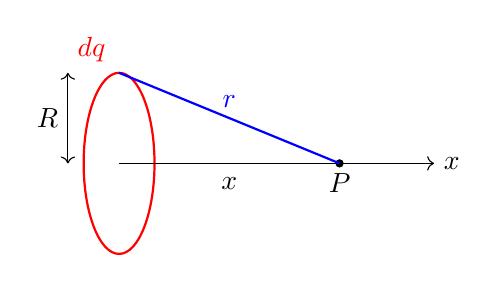
\begin{tikzpicture}[scale=1]
\draw[red,thick] (0,0) ellipse (0.45 and 1.15);
\draw[->] (0,0) -- (4,0) node[right] {\(x\)};
\fill (2.8,0) circle (1.5pt) node[below] {\(P\)};
\draw[blue,thick] (0,1.15) -- (2.8,0) node[midway,above] {\(r\)};
\draw[<->] (-0.65,0) -- (-0.65,1.15) node[midway,left] {\(R\)};
\node[red] at (-0.35,1.45) {\(dq\)};
\node at (1.4,-0.25) {\(x\)};
\end{tikzpicture}\end{center}

Ogni elemento dell'anello si trova alla stessa distanza dal punto \(P\):
\[
    r=\sqrt{x^2+R^2}.
\]
Quindi
\begin{align*}
V(x)
&=\int_{\text{anello}} \frac{1}{4\pi\varepsilon_0}\frac{dq}{\sqrt{x^2+R^2}} \\
&=\frac{1}{4\pi\varepsilon_0\sqrt{x^2+R^2}}\int_{\text{anello}}dq \\
&=\frac{q}{4\pi\varepsilon_0\sqrt{x^2+R^2}}.
\end{align*}

\begin{snippettheorem}{Potenziale sull'asse di un anello carico}
Il potenziale generato sull'asse di un anello uniformemente carico, di raggio \(R\) e carica totale \(q\), è
\[
    V(x)=\frac{q}{4\pi\varepsilon_0\sqrt{x^2+R^2}}.
\]
In particolare,
\[
    V(0)=\frac{q}{4\pi\varepsilon_0R}.
\]
\end{snippettheorem}

Per \(|x|\gg R\), si ha
\[
    \sqrt{x^2+R^2}\simeq |x|,
\]
e quindi
\[
    V(x)\simeq \frac{q}{4\pi\varepsilon_0|x|}.
\]
A grande distanza l'anello si comporta come una carica puntiforme \(q\).

\subsection{Campo elettrico sull'asse dell'anello}

Per simmetria, sull'asse dell'anello il campo elettrico ha solo componente lungo l'asse \(x\). Dunque
\[
    E_x(x)=-\frac{dV}{dx}.
\]
Usando
\[
    V(x)=\frac{q}{4\pi\varepsilon_0}(x^2+R^2)^{-1/2},
\]
otteniamo
\begin{align*}
E_x(x)
&=-\frac{d}{dx}\left[\frac{q}{4\pi\varepsilon_0}(x^2+R^2)^{-1/2}\right] \\
&=\frac{q}{4\pi\varepsilon_0}\frac{x}{(x^2+R^2)^{3/2}}.
\end{align*}

\begin{snippetproposition}{Campo sull'asse di un anello carico}
Il campo elettrico sull'asse dell'anello 
\[
    \vec{E}(x)=\frac{q}{4\pi\varepsilon_0}\frac{x}{(x^2+R^2)^{3/2}}\hat{u}_x.
\]
Nel centro dell'anello, \(x=0\), il campo è nullo per simmetria.
\end{snippetproposition}

\section{Potenziale sull'asse di un disco carico}

Consideriamo un disco di raggio \(R\), con densità superficiale uniforme \(\sigma\). Vogliamo calcolare il potenziale in un punto \(P\) sull'asse del disco, a distanza \(x\) dal centro.

\begin{center}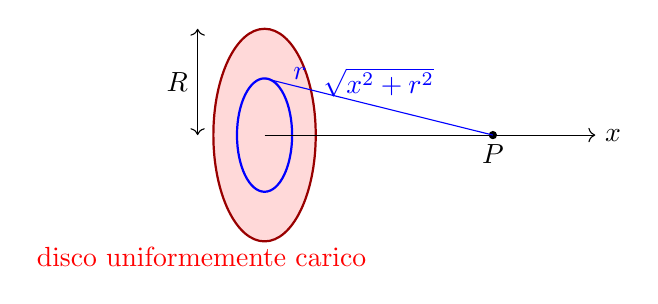
\begin{tikzpicture}[scale=1]
\draw[fill=red!15,draw=red!60!black,thick] (0,0) ellipse (0.65 and 1.35);
\draw[blue,thick] (0,0) ellipse (0.35 and 0.72);
\draw[->] (0,0) -- (4.2,0) node[right] {\(x\)};
\fill (2.9,0) circle (1.5pt) node[below] {\(P\)};
\draw[blue] (0,0.72) -- (2.9,0) node[midway,above] {\(\sqrt{x^2+r^2}\)};
\draw[<->] (-0.85,0) -- (-0.85,1.35) node[midway,left] {\(R\)};
\node[blue] at (0.45,0.78) {\(r\)};
\node[red] at (-0.8,-1.55) {disco uniformemente carico};
\end{tikzpicture}\end{center}

Scomponiamo il disco in anelli concentrici di raggio \(r\) e spessore \(dr\). L'area di un anello infinitesimo è
\[
    d\Sigma=2\pi r\,dr.
\]
La carica dell'anello è
\[
    dq=\sigma\,d\Sigma=2\pi\sigma r\,dr.
\]
Il contributo al potenziale del punto \(P\) è
\[
    dV=\frac{1}{4\pi\varepsilon_0}\frac{dq}{\sqrt{x^2+r^2}}.
\]
Quindi
\begin{align*}
V(x)
&=\int_0^R \frac{1}{4\pi\varepsilon_0}\frac{2\pi\sigma r\,dr}{\sqrt{x^2+r^2}} \\
&=\frac{\sigma}{2\varepsilon_0}\int_0^R \frac{r}{\sqrt{x^2+r^2}}\,dr.
\end{align*}
Poniamo
\[
    y=x^2+r^2,
\qquad
dy=2r\,dr.
\]
Allora
\[
    \int \frac{r}{\sqrt{x^2+r^2}}\,dr=\sqrt{x^2+r^2}.
\]
Pertanto
\begin{align*}
V(x)
&=\frac{\sigma}{2\varepsilon_0}\left[\sqrt{x^2+r^2}\right]_0^R \\
&=\frac{\sigma}{2\varepsilon_0}\left(\sqrt{x^2+R^2}-|x|\right).
\end{align*}

\begin{snippettheorem}{Potenziale sull'asse di un disco carico}
Il potenziale sull'asse di un disco uniformemente carico, di raggio \(R\) e densità superficiale \(\sigma\), è
\[
    V(x)=\frac{\sigma}{2\varepsilon_0}\left(\sqrt{x^2+R^2}-|x|\right).
\]
In particolare,
\[
    V(0)=\frac{\sigma R}{2\varepsilon_0}.
\]
\end{snippettheorem}

Per \(|x|\gg R\), usando
\[
    \sqrt{x^2+R^2}=|x|\sqrt{1+\frac{R^2}{x^2}}
\simeq |x|+\frac{R^2}{2|x|},
\]
si ottiene
\[
    V(x)\simeq \frac{\sigma}{2\varepsilon_0}\frac{R^2}{2|x|}
=\frac{\sigma\pi R^2}{4\pi\varepsilon_0|x|}.
\]
Poiché \(q=\sigma\pi R^2\), il disco lontano si comporta come una carica puntiforme:
\[
    V(x)\simeq \frac{q}{4\pi\varepsilon_0|x|}.
\]

\subsection{Campo elettrico sull'asse del disco}

Il campo lungo l'asse 
\[
    E_x(x)=-\frac{dV}{dx}.
\]
Poiché
\[
    \frac{d}{dx}|x|=\operatorname{sgn}(x)
=\begin{cases}
1, & x>0,\\
-1, & x<0,
\end{cases}
\]
abbiamo
\begin{align*}
E_x(x)
&=-\frac{d}{dx}\left[\frac{\sigma}{2\varepsilon_0}\left(\sqrt{x^2+R^2}-|x|\right)\right] \\
&=\frac{\sigma}{2\varepsilon_0}\left(\operatorname{sgn}(x)-\frac{x}{\sqrt{x^2+R^2}}\right).
\end{align*}

\begin{snippetproposition}{Campo sull'asse di un disco carico}
Il campo elettrico sull'asse del disco 
\[
    E_x(x)=\frac{\sigma}{2\varepsilon_0}\left(\operatorname{sgn}(x)-\frac{x}{\sqrt{x^2+R^2}}\right).
\]
Per \(x>0\), diventa
\[
    E_x(x)=\frac{\sigma}{2\varepsilon_0}\left(1-\frac{x}{\sqrt{x^2+R^2}}\right).
\]
\end{snippetproposition}

Nel punto \(x=0\) il potenziale ha una cuspide, quindi la derivata non è definita. Questo corrisponde al salto del campo attraversando il disco carico.

\section{Limite del piano infinito carico}

Il piano infinito carico si ottiene come limite di un disco di raggio \(R\) quando
\[
    R\to\infty.
\]
Se consideriamo punti vicini al centro e con \(|x|\ll R\), il termine
\[
    \frac{x}{\sqrt{x^2+R^2}}
\]
tende a zero. Quindi, per \(x>0\),
\[
    E_x(x)\to \frac{\sigma}{2\varepsilon_0},
\]
mentre, per \(x<0\),
\[
    E_x(x)\to -\frac{\sigma}{2\varepsilon_0}.
\]

\begin{snippettheorem}{Campo di un piano infinito uniformemente carico}
Un piano infinito con densità superficiale uniforme \(\sigma\) genera un campo elettrico costante, perpendicolare al piano:
\[
    \vec{E}=\begin{cases}
\displaystyle \frac{\sigma}{2\varepsilon_0}\hat{u}_x, & x>0,\\[6pt]
\displaystyle -\frac{\sigma}{2\varepsilon_0}\hat{u}_x, & x<0.
\end{cases}
\]
Il campo ha modulo
\[
    E=\frac{\sigma}{2\varepsilon_0}.
\]
\end{snippettheorem}

Nel limite del piano infinito, il potenziale del disco contiene un termine che diverge con \(R\). Tale termine è una costante additiva e non ha significato fisico. Infatti il campo dipende dalla derivata del potenziale, non dal valore assoluto del potenziale. Eliminando la costante, vicino al piano si ottiene
\[
    V(x)=V(0)-\frac{\sigma}{2\varepsilon_0}|x|.
\]

\begin{center}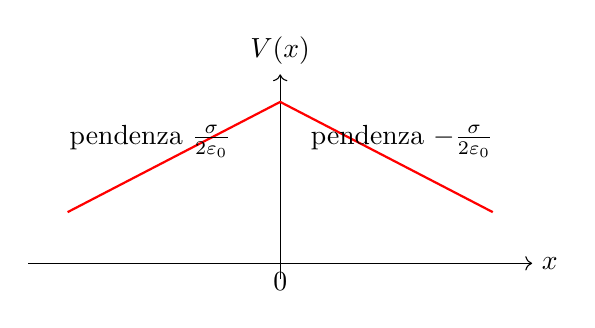
\begin{tikzpicture}[scale=1]
\draw[->] (-3.2,0) -- (3.2,0) node[right] {\(x\)};
\draw[->] (0,-0.2) -- (0,2.4) node[above] {\(V(x)\)};
\draw[red,thick] (-2.7,0.65) -- (0,2.05) -- (2.7,0.65);
\node[below] at (0,0) {\(0\)};
\node at (1.55,1.55) {pendenza \(-\frac{\sigma}{2\varepsilon_0}\)};
\node at (-1.65,1.55) {pendenza \(\frac{\sigma}{2\varepsilon_0}\)};
\end{tikzpicture}\end{center}

\section{Due piani infiniti con carica opposta}

Consideriamo due piani infiniti paralleli, con densità superficiali di carica opposte:
\[
    +\sigma,
\qquad
-\sigma.
\]
Tra i due piani i campi prodotti dalle due superfici hanno lo stesso verso e si sommano. All'esterno, invece, hanno versi opposti e si cancellano.

\begin{center}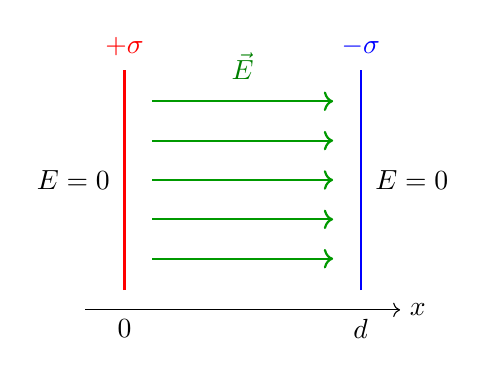
\begin{tikzpicture}[scale=1]
\draw[thick,red] (0,-1.4) -- (0,1.4);
\draw[thick,blue] (3,-1.4) -- (3,1.4);
\node[red] at (0,1.7) {\(+\sigma\)};
\node[blue] at (3,1.7) {\(-\sigma\)};
\foreach \y in {-1.0,-0.5,0,0.5,1.0}{
\draw[->,green!60!black,thick] (0.35,\y) -- (2.65,\y);
}
\node[green!50!black] at (1.5,1.45) {\(\vec{E}\)};
\node at (-0.65,0) {\(E=0\)};
\node at (3.65,0) {\(E=0\)};
\draw[->] (-0.5,-1.65) -- (3.5,-1.65) node[right] {\(x\)};
\node[below] at (0,-1.65) {\(0\)};
\node[below] at (3,-1.65) {\(d\)};
\end{tikzpicture}\end{center}

Nel tratto tra i due piani il modulo del campo è
\[
    E=\frac{\sigma}{2\varepsilon_0}+\frac{\sigma}{2\varepsilon_0}=\frac{\sigma}{\varepsilon_0}.
\]
Fuori dai piani si ha
\[
    E=0.
\]

Se scegliamo l'asse \(x\) perpendicolare ai piani, con il piano positivo in \(x=0\) e quello negativo in \(x=d\), allora tra i piani
\[
    E_x=\frac{\sigma}{\varepsilon_0}.
\]
Poiché
\[
    E_x=-\frac{dV}{dx},
\]
si ottiene
\[
    \frac{dV}{dx}=-\frac{\sigma}{\varepsilon_0}.
\]
Quindi
\[
    V(x)=V(0)-\frac{\sigma}{\varepsilon_0}x
\qquad 0<x<d.
\]

\begin{snippetproposition}{Potenziale tra due piani infiniti opposti}
Tra due piani infiniti paralleli con densità \(+\sigma\) e \(-\sigma\), il campo elettrico è uniforme:
\[
    E=\frac{\sigma}{\varepsilon_0}.
\]
Il potenziale decresce linearmente:
\[
    V(x)=V(0)-\frac{\sigma}{\varepsilon_0}x.
\]
Fuori dai piani il campo è nullo e il potenziale è costante.
\end{snippetproposition}

\begin{center}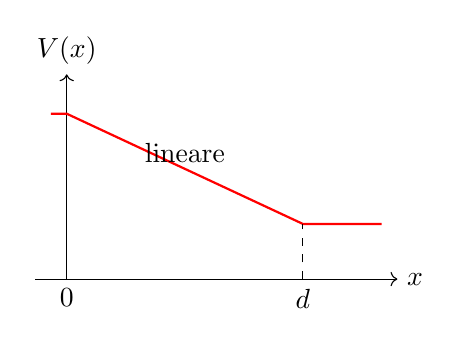
\begin{tikzpicture}[scale=1]
\draw[->] (-0.4,0) -- (4.2,0) node[right] {\(x\)};
\draw[->] (0,0) -- (0,2.6) node[above] {\(V(x)\)};
\draw[red,thick] (-0.2,2.1) -- (0,2.1) -- (3,0.7) -- (4,0.7);
\draw[dashed] (3,0) -- (3,0.7);
\node[below] at (0,0) {\(0\)};
\node[below] at (3,0) {\(d\)};
\node at (1.5,1.6) {lineare};
\end{tikzpicture}\end{center}

\section{Differenziale del potenziale in tre dimensioni}

In una dimensione, la relazione tra campo elettrico e potenziale è
\[
    E_x=-\frac{dV}{dx}.
\]
In tre dimensioni il potenziale è una funzione
\[
    V=V(x,y,z).
\]
Il suo differenziale è
\[
    dV=\frac{\partial V}{\partial x}dx+\frac{\partial V}{\partial y}dy+\frac{\partial V}{\partial z}dz.
\]
D'altra parte il lavoro elementare della forza elettrica su una carica \(q\) è
\[
    dW=\vec{F}_e\cdot d\vec{s}=q\vec{E}\cdot d\vec{s}.
\]
Poiché
\[
    dW=-dU_e=-q\,dV,
\]
si ha
\[
    q\vec{E}\cdot d\vec{s}=-q\,dV.
\]
Dividendo per \(q\):
\[
    \vec{E}\cdot d\vec{s}=-dV.
\]
Scrivendo
\[
    \vec{E}=E_x\hat{u}_x+E_y\hat{u}_y+E_z\hat{u}_z,
\qquad
d\vec{s}=dx\hat{u}_x+dy\hat{u}_y+dz\hat{u}_z,
\]
si ottiene
\[
    E_xdx+E_ydy+E_zdz
=-\left(\frac{\partial V}{\partial x}dx+\frac{\partial V}{\partial y}dy+\frac{\partial V}{\partial z}dz\right).
\]
Confrontando i coefficienti di \(dx\), \(dy\), \(dz\), segue
\[
    E_x=-\frac{\partial V}{\partial x},
\qquad
E_y=-\frac{\partial V}{\partial y},
\qquad
E_z=-\frac{\partial V}{\partial z}.
\]

\begin{snippetdefinition}{Gradiente}
Il gradiente di una funzione scalare \(V(x,y,z)\) è il campo vettoriale
\[
    \vec{\nabla}V=\frac{\partial V}{\partial x}\hat{u}_x+\frac{\partial V}{\partial y}\hat{u}_y+\frac{\partial V}{\partial z}\hat{u}_z.
\]
\end{snippetdefinition}

Quindi il campo elettrico è l'opposto del gradiente del potenziale:
\[
    \vec{E}=-\vec{\nabla}V.
\]

\begin{snippettheorem}{Campo elettrico come gradiente del potenziale}
In elettrostatica, il campo elettrico è dato da
\[
    \vec{E}=-\vec{\nabla}V.
\]
In coordinate cartesiane:
\[
    \vec{E}
=-\frac{\partial V}{\partial x}\hat{u}_x
-\frac{\partial V}{\partial y}\hat{u}_y
-\frac{\partial V}{\partial z}\hat{u}_z.
\]
\end{snippettheorem}

Questa formula generalizza la relazione monodimensionale \(E=-dV/dx\). Il campo punta verso le regioni dove il potenziale diminuisce più rapidamente.

\section{Richiamo sui vettori}

Prima di introdurre altri operatori differenziali, richiamiamo le operazioni fondamentali tra vettori.

\subsection{Prodotto scalare}

Per due vettori \(
\vec{A}\) e \(\vec{B}\), il prodotto scalare è
\[
    \vec{A}\cdot\vec{B}=AB\cos\theta.
\]
In coordinate cartesiane:
\[
    \vec{A}\cdot\vec{B}=A_xB_x+A_yB_y+A_zB_z.
\]
Il risultato è uno scalare.

\subsection{Prodotto vettoriale}

Il prodotto vettoriale tra \(\vec{A}\) e \(\vec{B}\) è un vettore perpendicolare sia a \(\vec{A}\) sia a \(\vec{B}\). Il suo modulo è
\[
    |\vec{A}\times\vec{B}|=AB\sin\theta.
\]
Il verso è dato dalla regola della mano destra. In coordinate cartesiane:
\[
    \vec{A}\times\vec{B}
=\begin{vmatrix}
\hat{u}_x & \hat{u}_y & \hat{u}_z \\
A_x & A_y & A_z \\
B_x & B_y & B_z
\end{vmatrix}.
\]
Sviluppando:
\[
    \vec{A}\times\vec{B}
=(A_yB_z-B_yA_z)\hat{u}_x
-(A_xB_z-B_xA_z)\hat{u}_y
+(A_xB_y-B_xA_y)\hat{u}_z.
\]

\section{Rotore di un campo vettoriale}

L'operatore nabla è
\[
    \vec{\nabla}=\left(\frac{\partial}{\partial x},\frac{\partial}{\partial y},\frac{\partial}{\partial z}\right).
\]
Se \(\vec{A}=A_x\hat{u}_x+A_y\hat{u}_y+A_z\hat{u}_z\), il rotore di \(\vec{A}\) è il prodotto vettoriale formale tra \(\vec{\nabla}\) e \(\vec{A}\):
\[
    \vec{\nabla}\times\vec{A}
=\begin{vmatrix}
\hat{u}_x & \hat{u}_y & \hat{u}_z \\
\partial_x & \partial_y & \partial_z \\
A_x & A_y & A_z
\end{vmatrix}.
\]
Quindi
\[
    \vec{\nabla}\times\vec{A}
=\left(\frac{\partial A_z}{\partial y}-\frac{\partial A_y}{\partial z}\right)\hat{u}_x
-\left(\frac{\partial A_z}{\partial x}-\frac{\partial A_x}{\partial z}\right)\hat{u}_y
+\left(\frac{\partial A_y}{\partial x}-\frac{\partial A_x}{\partial y}\right)\hat{u}_z.
\]

\begin{snippetdefinition}{Rotore}
Il rotore di un campo vettoriale \(\vec{A}\) è il campo vettoriale
\[
    \operatorname{rot}\vec{A}=\vec{\nabla}\times\vec{A}.
\]
Esso misura localmente la tendenza del campo a produrre circuitazione attorno a un punto.
\end{snippetdefinition}

\section{Riassunto degli operatori differenziali}

Gli operatori principali costruiti con \(\vec{\nabla}\) sono:
\begin{itemize}
\item gradiente di una funzione scalare:
\[
    \vec{\nabla}V=\operatorname{grad}V,
\qquad
\realnumbers^3\to\realnumbers^3;
\]
\item divergenza di un campo vettoriale:
\[
    \vec{\nabla}\cdot\vec{A}=\operatorname{div}\vec{A},
\qquad
\realnumbers^3\to\realnumbers;
\]
\item rotore di un campo vettoriale:
\[
    \vec{\nabla}\times\vec{A}=\operatorname{rot}\vec{A},
\qquad
\realnumbers^3\to\realnumbers^3;
\]
\item laplaciano di una funzione scalare:
\[
    \nabla^2V=\vec{\nabla}\cdot(\vec{\nabla}V).
\]
\end{itemize}

La divergenza individua sorgenti e pozzi di un campo, mentre il rotore individua la tendenza del campo a circolare.

\begin{center}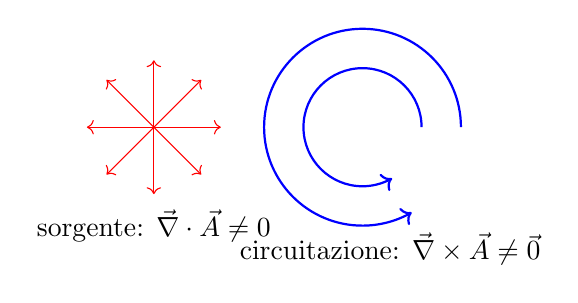
\begin{tikzpicture}[scale=1]
\foreach \a in {0,45,...,315}{
\draw[->,red] (0,0) -- ({0.85*cos(\a)},{0.85*sin(\a)});
}
\node at (0,-1.25) {sorgente: \(\vec{\nabla}\cdot\vec{A}\neq0\)};
\draw[->,blue,thick] (3.4,0) arc (0:300:0.75);
\draw[->,blue,thick] (3.9,0) arc (0:300:1.25);
\node at (3,-1.55) {circuitazione: \(\vec{\nabla}\times\vec{A}\neq\vec{0}\)};
\end{tikzpicture}\end{center}

Nel campo elettrico elettrostatico le cariche sono sorgenti del campo, mentre il rotore è nullo. Nel campo magnetico, invece, le correnti sono associate alla circuitazione del campo.

\section{Teorema del rotore nullo}

\begin{snippettheorem}{Campo irrotazionale e potenziale scalare}
Se un campo vettoriale \(\vec{A}\) soddisfa
\[
    \vec{\nabla}\times\vec{A}=\vec{0},
\]
allora, almeno localmente in una regione semplicemente connessa, esiste una funzione scalare \(\varphi\) tale che
\[
    \vec{A}=\vec{\nabla}\varphi.
\]
\end{snippettheorem}

In altre parole, un campo irrotazionale può essere scritto come gradiente di un potenziale scalare.

\begin{snippetproof}{Verifica che il gradiente ha rotore nullo}
Supponiamo che
\[
    \vec{A}=\vec{\nabla}\varphi.
\]
Allora
\[
    \vec{A}=\frac{\partial\varphi}{\partial x}\hat{u}_x+\frac{\partial\varphi}{\partial y}\hat{u}_y+\frac{\partial\varphi}{\partial z}\hat{u}_z.
\]
Calcoliamo il rotore:
\[
    \vec{\nabla}\times\vec{A}
=\begin{vmatrix}
\hat{u}_x & \hat{u}_y & \hat{u}_z \\
\partial_x & \partial_y & \partial_z \\
\partial_x\varphi & \partial_y\varphi & \partial_z\varphi
\end{vmatrix}.
\]
La componente \(z\), per esempio, è
\[
    \frac{\partial^2\varphi}{\partial x\partial y}
-\frac{\partial^2\varphi}{\partial y\partial x}=0,
\]
per l'uguaglianza delle derivate miste. Analogamente si annullano le altre componenti, quindi
\[
    \vec{\nabla}\times\left(\vec{\nabla}\varphi\right)=\vec{0}.
\]
\end{snippetproof}

Applicando questo risultato al campo elettrico elettrostatico, poiché
\[
    \vec{E}=-\vec{\nabla}V,
\]
si ha
\[
    \vec{\nabla}\times\vec{E}=\vec{0}.
\]
Questa è la forma locale della conservatività del campo elettrico.


\pagebreak
\part{Lezione 6}

\section{Operatori vettoriali}

In elettrostatica e, pi in generale, nello studio dei campi,  utile introdurre alcuni operatori differenziali. In coordinate cartesiane si definisce l'operatore nabla come
\[
    \vec{\nabla}=\left(\frac{\partial}{\partial x},\frac{\partial}{\partial y},\frac{\partial}{\partial z}\right).
\]
Spesso si scrive anche
\[
    \partial_x=\frac{\partial}{\partial x},
\qquad
\partial_y=\frac{\partial}{\partial y},
\qquad
\partial_z=\frac{\partial}{\partial z}.
\]

\subsection{Gradiente}

Se \(V=V(x,y,z)\) è una funzione scalare, il suo gradiente è il campo vettoriale
\[
    \vec{\nabla}V=\frac{\partial V}{\partial x}\hat{u}_x+\frac{\partial V}{\partial y}\hat{u}_y+\frac{\partial V}{\partial z}\hat{u}_z.
\]
Il gradiente indica la direzione di massima crescita della funzione \(V\).

In elettrostatica il campo elettrico è legato al potenziale da
\[
    \vec{E}=-\vec{\nabla}V.
\]

\subsection{Divergenza}

Se \(\vec{E}=E_x\hat{u}_x+E_y\hat{u}_y+E_z\hat{u}_z\), la divergenza di \(\vec{E}\) è
\[
    \vec{\nabla}\cdot\vec{E}
=\frac{\partial E_x}{\partial x}+\frac{\partial E_y}{\partial y}+\frac{\partial E_z}{\partial z}.
\]
La divergenza misura localmente quanto un campo tende a uscire da un punto. Nel caso del campo elettrico, le sorgenti della divergenza sono le cariche elettriche.

\subsection{Rotore}

Il rotore di un campo vettoriale \(\vec{E}\) è
\[
    \vec{\nabla}\times\vec{E}
=\begin{vmatrix}
\hat{u}_x & \hat{u}_y & \hat{u}_z \\
\partial_x & \partial_y & \partial_z \\
E_x & E_y & E_z
\end{vmatrix}.
\]
Sviluppando il determinante:
\[
    \vec{\nabla}\times\vec{E}
=\left(\frac{\partial E_z}{\partial y}-\frac{\partial E_y}{\partial z}\right)\hat{u}_x
-\left(\frac{\partial E_z}{\partial x}-\frac{\partial E_x}{\partial z}\right)\hat{u}_y
+\left(\frac{\partial E_y}{\partial x}-\frac{\partial E_x}{\partial y}\right)\hat{u}_z.
\]
Il rotore misura localmente la tendenza del campo a ``girare'' attorno a un punto.

\subsection{Laplaciano}

Il laplaciano è l'operatore scalare
\[
    \nabla^2=\frac{\partial^2}{\partial x^2}+\frac{\partial^2}{\partial y^2}+\frac{\partial^2}{\partial z^2}.
\]
Applicato a una funzione scalare \(V\), dà
\[
    \nabla^2V=\frac{\partial^2V}{\partial x^2}+\frac{\partial^2V}{\partial y^2}+\frac{\partial^2V}{\partial z^2}.
\]

\section{Teorema del rotore del gradiente}

\begin{snippettheorem}{Rotore del gradiente}
Per ogni funzione scalare regolare \(V\), vale
\[
    \vec{\nabla}\times\left(\vec{\nabla}V\right)=\vec{0}.
\]
\end{snippettheorem}

\begin{snippetproof}{Verifica della componente \(x\)}
Calcoliamo la componente \(x\) del rotore del gradiente. Poiché
\[
    \vec{\nabla}V=\frac{\partial V}{\partial x}\hat{u}_x+\frac{\partial V}{\partial y}\hat{u}_y+\frac{\partial V}{\partial z}\hat{u}_z,
\]
si ha
\[
    \left[\vec{\nabla}\times\left(\vec{\nabla}V\right)\right]_x
=\frac{\partial}{\partial y}\left(\frac{\partial V}{\partial z}\right)
-\frac{\partial}{\partial z}\left(\frac{\partial V}{\partial y}\right).
\]
Se \(V\) è regolare, le derivate miste si possono scambiare:
\[
    \frac{\partial^2V}{\partial y\partial z}
=\frac{\partial^2V}{\partial z\partial y}.
\]
Quindi la componente \(x\) è nulla. Lo stesso ragionamento vale per le componenti \(y\) e \(z\), e dunque
\[
    \vec{\nabla}\times\left(\vec{\nabla}V\right)=\vec{0}.
\]
\end{snippetproof}

Nel caso elettrostatico,
\[
    \vec{E}=-\vec{\nabla}V.
\]
Allora
\[
    \vec{\nabla}\times\vec{E}
=\vec{\nabla}\times\left(-\vec{\nabla}V\right)
=-\vec{\nabla}\times\left(\vec{\nabla}V\right)=\vec{0}.
\]

\begin{snippetproposition}{Campo elettrostatico irrotazionale}
Un campo elettrico elettrostatico è conservativo e quindi irrotazionale:
\[
    \vec{E}=-\vec{\nabla}V
\qquad\Longrightarrow\qquad
\vec{\nabla}\times\vec{E}=\vec{0}.
\]
\end{snippetproposition}

Questa proprietà vale per campi statici. Se invece i campi dipendono dal tempo, la situazione cambia: in elettrodinamica la legge di Faraday diventa
\[
    \vec{\nabla}\times\vec{E}=-\frac{\partial\vec{B}}{\partial t},
\]
dove \(\vec{B}\) è il campo magnetico. Quindi un campo magnetico variabile nel tempo genera un campo elettrico con rotore non nullo.

\section{Potenziale elettrico di un dipolo}

Consideriamo un dipolo elettrico formato da due cariche puntiformi \(+q\) e \(-q\), separate da una distanza \(a\). Il momento di dipolo è definito come
\[
    \vec{p}=q\vec{a},
\]
dove \(\vec{a}\) è il vettore diretto dalla carica negativa alla carica positiva. Il suo modulo è
\[
    p=qa.
\]

Vogliamo calcolare il potenziale in un punto \(P\) lontano dal dipolo. Scegliamo l'origine nel punto medio del dipolo e indichiamo con \(r_1\) la distanza di \(P\) dalla carica positiva, e con \(r_2\) la distanza di \(P\) dalla carica negativa.

\begin{center}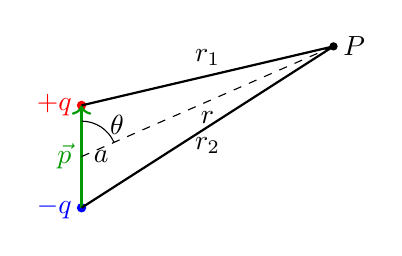
\begin{tikzpicture}[scale=1]
\coordinate (O) at (0,0);
\coordinate (M) at (0,-0.65);
\coordinate (P) at (3.2,1.4);
\fill[red] (0,0.65) circle (1.7pt) node[left] {\(+q\)};
\fill[blue] (0,-0.65) circle (1.7pt) node[left] {\(-q\)};
\draw[->,green!60!black,thick] (0,-0.65) -- (0,0.65) node[midway,left] {\(\vec{p}\)};
\draw[thick] (0,0.65) -- (P) node[midway,above] {\(r_1\)};
\draw[thick] (0,-0.65) -- (P) node[midway,below] {\(r_2\)};
\draw[dashed] (O) -- (P) node[midway,below] {\(r\)};
\draw (0,0.45) arc (90:24:0.45);
\node at (0.45,0.4) {\(\theta\)};
\fill (P) circle (1.5pt) node[right] {\(P\)};
\node at (0.25,0) {\(a\)};
\end{tikzpicture}\end{center}

Il potenziale nel punto \(P\) è la somma dei potenziali prodotti dalle due cariche:
\[
    V(P)=\frac{q}{4\pi\varepsilon_0r_1}-\frac{q}{4\pi\varepsilon_0r_2}.
\]
Quindi
\[
    V(P)=\frac{q}{4\pi\varepsilon_0}\left(\frac{1}{r_1}-\frac{1}{r_2}\right)
=\frac{q}{4\pi\varepsilon_0}\frac{r_2-r_1}{r_1r_2}.
\]

\subsection{Espressione in coordinate polari}

Indichiamo con \(\theta\) l'angolo tra \(\vec{p}\) e il vettore posizione \(\vec{r}\) del punto \(P\). Dal teorema del coseno si ottiene
\[
    r_1^2=r^2+\frac{a^2}{4}-ar\cos\theta,
\]
mentre
\[
    r_2^2=r^2+\frac{a^2}{4}+ar\cos\theta.
\]
Sottraendo le due relazioni:
\[
    r_2^2-r_1^2=2ar\cos\theta.
\]
Poiché
\[
    r_2^2-r_1^2=(r_2-r_1)(r_2+r_1),
\]
abbiamo
\[
    (r_2-r_1)(r_2+r_1)=2ar\cos\theta.
\]

Se il punto \(P\) è molto lontano rispetto alla distanza tra le cariche, cioè
\[
    r\gg a,
\]
allora
\[
    r_1+r_2\simeq 2r,
\qquad
r_1r_2\simeq r^2.
\]
Quindi
\[
    r_2-r_1\simeq a\cos\theta.
\]
Sostituendo nell'espressione del potenziale:
\[
    V(r,\theta)\simeq \frac{q}{4\pi\varepsilon_0}\frac{a\cos\theta}{r^2}.
\]
Poiché \(p=qa\), otteniamo
\[
    V(r,\theta)=\frac{p\cos\theta}{4\pi\varepsilon_0r^2}
\qquad\text{per } r\gg a.
\]

\begin{snippettheorem}{Potenziale del dipolo elettrico}
A grande distanza da un dipolo elettrico, cioè per \(r\gg a\), il potenziale è
\[
    V(r,\theta)=\frac{p\cos\theta}{4\pi\varepsilon_0r^2}.
\]
Equivalentemente,
\[
    V(\vec{r})=\frac{\vec{p}\cdot\hat{r}}{4\pi\varepsilon_0r^2}
=\frac{\vec{p}\cdot\vec{r}}{4\pi\varepsilon_0r^3}.
\]
\end{snippettheorem}

Il potenziale del dipolo decresce come \(1/r^2\), più rapidamente del potenziale di una carica puntiforme, che decresce come \(1/r\). Questo è coerente con il fatto che la carica totale del dipolo è nulla.

\section{Campo elettrico del dipolo}

Per ottenere il campo elettrico del dipolo partiamo dalla relazione
\[
    \vec{E}=-\vec{\nabla}V.
\]
In coordinate polari piane \((r,\theta)\), quando il potenziale non dipende dall'angolo azimutale, il gradiente è
\[
    \vec{\nabla}V=\frac{\partial V}{\partial r}\hat{u}_r+\frac{1}{r}\frac{\partial V}{\partial\theta}\hat{u}_\theta.
\]
Dunque
\[
    \vec{E}=-\frac{\partial V}{\partial r}\hat{u}_r-\frac{1}{r}\frac{\partial V}{\partial\theta}\hat{u}_\theta.
\]

Usando
\[
    V(r,\theta)=\frac{p\cos\theta}{4\pi\varepsilon_0r^2},
\]
calcoliamo le due componenti.

Per la componente radiale:
\begin{align*}
E_r
&=-\frac{\partial}{\partial r}\left(\frac{p\cos\theta}{4\pi\varepsilon_0r^2}\right) \\
&=-\frac{p\cos\theta}{4\pi\varepsilon_0}\frac{\partial}{\partial r}\left(r^{-2}\right) \\
&=\frac{2p\cos\theta}{4\pi\varepsilon_0r^3}.
\end{align*}
Per la componente angolare:
\begin{align*}
E_\theta
&=-\frac{1}{r}\frac{\partial}{\partial\theta}\left(\frac{p\cos\theta}{4\pi\varepsilon_0r^2}\right) \\
&=-\frac{1}{r}\frac{p}{4\pi\varepsilon_0r^2}(-\sin\theta) \\
&=\frac{p\sin\theta}{4\pi\varepsilon_0r^3}.
\end{align*}

Quindi
\[
    \vec{E}(r,\theta)=\frac{p}{4\pi\varepsilon_0r^3}\left(2\cos\theta\,\hat{u}_r+\sin\theta\,\hat{u}_\theta\right).
\]

\begin{snippettheorem}{Campo elettrico del dipolo}
A grande distanza da un dipolo elettrico, cioè per \(r\gg a\), il campo elettrico è
\[
    \vec{E}(r,\theta)=\frac{p}{4\pi\varepsilon_0r^3}\left(2\cos\theta\,\hat{u}_r+\sin\theta\,\hat{u}_\theta\right).
\]
Il campo del dipolo decresce come \(1/r^3\).
\end{snippettheorem}

\begin{center}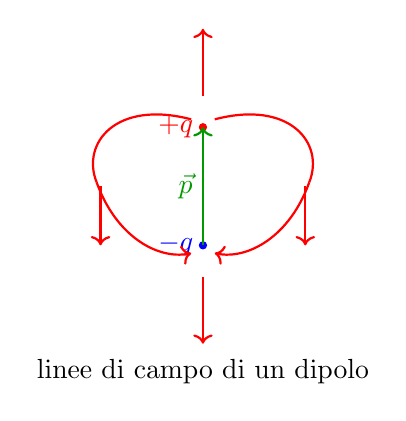
\begin{tikzpicture}[scale=1]
\fill[red] (0,0.75) circle (1.5pt) node[left] {\(+q\)};
\fill[blue] (0,-0.75) circle (1.5pt) node[left] {\(-q\)};
\draw[->,green!60!black,thick] (0,-0.75) -- (0,0.75) node[midway,left] {\(\vec{p}\)};
\draw[->,red,thick] (0,1.15) -- (0,2.0);
\draw[->,red,thick] (0,-1.15) -- (0,-2.0);
\draw[->,red,thick] (1.3,0) -- (1.3,-0.75);
\draw[->,red,thick] (-1.3,0) -- (-1.3,-0.75);
\draw[red,thick] (0.15,0.85) .. controls (1.1,1.1) and (1.55,0.55) .. (1.35,0.05);
\draw[red,thick,->] (1.35,0.05) .. controls (1.1,-0.65) and (0.55,-0.95) .. (0.15,-0.85);
\draw[red,thick] (-0.15,0.85) .. controls (-1.1,1.1) and (-1.55,0.55) .. (-1.35,0.05);
\draw[red,thick,->] (-1.35,0.05) .. controls (-1.1,-0.65) and (-0.55,-0.95) .. (-0.15,-0.85);
\node at (0,-2.35) {linee di campo di un dipolo};
\end{tikzpicture}\end{center}

\subsection{Valori del campo lungo assi notevoli}

Sull'asse del dipolo sopra la carica positiva si ha \(\theta=0\). Quindi
\[
    \cos\theta=1,
\qquad
\sin\theta=0,
\]
e
\[
    \vec{E}=\frac{2p}{4\pi\varepsilon_0r^3}\hat{u}_r.
\]
Il campo è diretto come \(\vec{p}\).

Sull'asse del dipolo sotto la carica negativa si ha \(\theta=\pi\). Quindi
\[
    \cos\theta=-1,
\qquad
\sin\theta=0,
\]
e il campo ha ancora direzione complessiva concorde con l'asse del dipolo, ma verso opposto al versore radiale locale.

Sul piano equatoriale del dipolo si ha
\[
    \theta=\frac{\pi}{2}
\qquad\text{oppure}\qquad
\theta=\frac{3\pi}{2}.
\]
In entrambi i casi \(\cos\theta=0\), quindi il campo non ha componente radiale. Il campo è diretto in verso opposto a \(\vec{p}\) e ha modulo
\[
    E=\frac{p}{4\pi\varepsilon_0r^3}.
\]

\section{Dipolo in un campo elettrico uniforme}

Consideriamo un dipolo elettrico immerso in un campo elettrico uniforme \(\vec{E}\). Sulla carica positiva agisce la forza
\[
    \vec{F}_+=q\vec{E},
\]
mentre sulla carica negativa agisce la forza
\[
    \vec{F}_-=-q\vec{E}.
\]
Le due forze hanno uguale modulo e verso opposto, quindi la forza totale è nulla:
\[
    \vec{F}_{\mathrm{tot}}=\vec{F}_++\vec{F}_-=\vec{0}.
\]
Tuttavia, se le due forze sono applicate in punti diversi, formano una coppia di forze e producono un momento torcente.

\begin{center}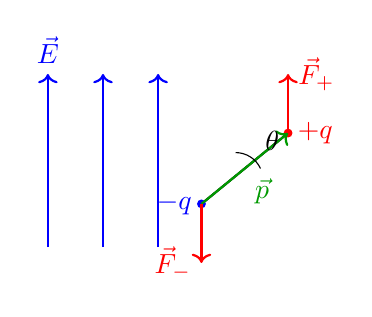
\begin{tikzpicture}[scale=1]
\draw[->,blue,thick] (-0.6,0) -- (-0.6,2.2) node[above] {\(\vec{E}\)};
\draw[->,blue,thick] (0.1,0) -- (0.1,2.2);
\draw[->,blue,thick] (0.8,0) -- (0.8,2.2);
\coordinate (M) at (1.9,1.0);
\coordinate (Pp) at (2.45,1.45);
\coordinate (Pm) at (1.35,0.55);
\draw[thick] (Pm) -- (Pp);
\fill[red] (Pp) circle (1.6pt) node[right] {\(+q\)};
\fill[blue] (Pm) circle (1.6pt) node[left] {\(-q\)};
\draw[->,green!60!black,thick] (Pm) -- (Pp) node[midway,below right] {\(\vec{p}\)};
\draw[->,red,thick] (Pp) -- ++(0,0.75) node[right] {\(\vec{F}_+\)};
\draw[->,red,thick] (Pm) -- ++(0,-0.75) node[left] {\(\vec{F}_-\)};
\draw (2.1,1.0) arc (25:90:0.35);
\node at (2.25,1.35) {\(\theta\)};
\end{tikzpicture}\end{center}

Il momento della forza totale rispetto all'origine è
\[
    \vec{M}=\vec{r}_+\times\vec{F}_+ + \vec{r}_-\times\vec{F}_-.
\]
Sostituendo \(\vec{F}_+=q\vec{E}\) e \(\vec{F}_-=-q\vec{E}\), si ottiene
\begin{align*}
\vec{M}
&=q\vec{r}_+\times\vec{E}-q\vec{r}_-\times\vec{E} \\
&=q(\vec{r}_+-\vec{r}_-)\times\vec{E}.
\end{align*}
Ma
\[
    q(\vec{r}_+-\vec{r}_-)=\vec{p}.
\]
Quindi
\[
    \vec{M}=\vec{p}\times\vec{E}.
\]

\begin{snippettheorem}{Momento torcente su un dipolo}
Un dipolo elettrico immerso in un campo elettrico uniforme subisce un momento torcente
\[
    \vec{M}=\vec{p}\times\vec{E}.
\]
Il modulo è
\[
    M=pE\sin\theta,
\]
dove \(\theta\) è l'angolo tra \(\vec{p}\) e \(\vec{E}\).
\end{snippettheorem}

La coppia di forze tende ad allineare il dipolo al campo elettrico. Se \(\theta=0\), il momento è nullo e il dipolo è in equilibrio stabile. Se \(\theta=\pi\), il momento è ancora nullo, ma l'equilibrio è instabile: una piccola perturbazione fa ruotare il dipolo verso l'allineamento con il campo.

\section{Energia potenziale di un dipolo in un campo uniforme}

Supponiamo che il campo elettrico uniforme sia diretto lungo l'asse \(y\):
\[
    \vec{E}=E\hat{u}_y.
\]
Poiché
\[
    \vec{E}=-\vec{\nabla}V,
\]
possiamo scegliere un potenziale della forma
\[
    V(y)=-Ey+C.
\]
La costante additiva non ha significato fisico e può essere scelta arbitrariamente.

Consideriamo un dipolo che forma un angolo \(\theta\) con il campo. Se il centro del dipolo ha coordinata \(y\), le coordinate delle due cariche sono
\[
    y_+=y+\frac{a}{2}\cos\theta,
\qquad
y_-=y-\frac{a}{2}\cos\theta.
\]
L'energia potenziale elettrica del dipolo è la somma delle energie delle due cariche:
\[
    U_e=qV(y_+)+(-q)V(y_-).
\]
Usando \(V(y)=-Ey+C\), otteniamo
\begin{align*}
U_e
&=q\left[-E\left(y+\frac{a}{2}\cos\theta\right)+C\right]
-q\left[-E\left(y-\frac{a}{2}\cos\theta\right)+C\right] \\
&=-qEy-\frac{qEa}{2}\cos\theta+qC
+qEy-\frac{qEa}{2}\cos\theta-qC \\
&=-qaE\cos\theta.
\end{align*}
Poiché \(p=qa\), segue
\[
    U_e=-pE\cos\theta.
\]
In forma vettoriale:
\[
    U_e=-\vec{p}\cdot\vec{E}.
\]

\begin{snippettheorem}{Energia potenziale di un dipolo}
L'energia potenziale di un dipolo elettrico in un campo elettrico uniforme è
\[
    U_e=-\vec{p}\cdot\vec{E}=-pE\cos\theta.
\]
\end{snippettheorem}

\begin{center}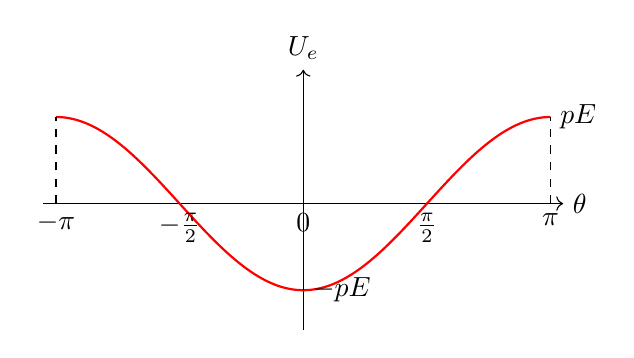
\begin{tikzpicture}[scale=1]
\draw[->] (-3.3,0) -- (3.3,0) node[right] {\(\theta\)};
\draw[->] (0,-1.6) -- (0,1.7) node[above] {\(U_e\)};
\draw[red,thick,domain=-3.14:3.14,samples=160] plot (\x,{-1.1*cos(57.2958*\x)});
\draw[dashed] (-3.14,0) -- (-3.14,1.1);
\draw[dashed] (3.14,0) -- (3.14,1.1);
\draw[dashed] (0,0) -- (0,-1.1);
\node[below] at (0,0) {\(0\)};
\node[below] at (1.57,0) {\(\frac{\pi}{2}\)};
\node[below] at (3.14,0) {\(\pi\)};
\node[below] at (-1.57,0) {\(-\frac{\pi}{2}\)};
\node[below] at (-3.14,0) {\(-\pi\)};
\node[right] at (0,-1.1) {\(-pE\)};
\node[right] at (3.14,1.1) {\(pE\)};
\end{tikzpicture}\end{center}

Il minimo dell'energia si ha per
\[
    \theta=0,
\]
cioè quando \(\vec{p}\) è parallelo e concorde a \(\vec{E}\). Questo è l'equilibrio stabile. Il massimo dell'energia si ha per
\[
    \theta=\pi,
\]
cioè quando \(\vec{p}\) è antiparallelo a \(\vec{E}\). Questo è l'equilibrio instabile.

\pagebreak
\part{Lezione 7}

\section{Flusso di un campo vettoriale}

Vogliamo introdurre una grandezza che misuri quante linee di campo attraversano una superficie. Consideriamo inizialmente il caso semplice di una superficie piana \(\Sigma\) immersa in un campo vettoriale uniforme \(\vec{E}\).

Sia \(\hat{n}\) il versore normale alla superficie. Se \(\theta\) è l'angolo tra \(\vec{E}\) e \(\hat{n}\), il flusso di \(\vec{E}\) attraverso \(\Sigma\) è
\[
    \Phi_\Sigma(\vec{E})=\vec{E}\cdot\hat{n}\,\Sigma
=E\Sigma\cos\theta.
\]

\begin{snippetdefinition}{Flusso attraverso una superficie piana}
Se \(\vec{E}\) è uniforme e \(\Sigma\) è una superficie piana orientata da \(\hat{n}\), il flusso di \(\vec{E}\) attraverso \(\Sigma\) è
\[
    \Phi_\Sigma(\vec{E})=\vec{E}\cdot\hat{n}\,\Sigma.
\]
\end{snippetdefinition}

\begin{center}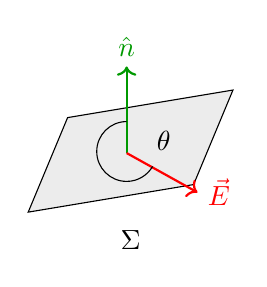
\begin{tikzpicture}[scale=1]
\draw[fill=gray!15,draw=black] (0,0) -- (2.1,0.35) -- (2.6,1.55) -- (0.5,1.2) -- cycle;
\draw[->,green!60!black,thick] (1.25,0.75) -- (1.25,1.85) node[above] {\(\hat{n}\)};
\draw[->,red,thick] (1.25,0.75) -- (2.15,0.25) node[right] {\(\vec{E}\)};
\draw (1.25,1.15) arc (90:330:0.38);
\node at (1.72,0.9) {\(\theta\)};
\node at (1.3,-0.35) {\(\Sigma\)};
\end{tikzpicture}\end{center}

Osserviamo alcuni casi particolari.

\begin{snippetexample}{Campo perpendicolare alla superficie}
Se \(\vec{E}\) è perpendicolare alla superficie, allora è parallelo a \(\hat{n}\). Quindi \(\theta=0\), \(\cos\theta=1\), e
\[
    \Phi_\Sigma(\vec{E})=E\Sigma.
\]
\end{snippetexample}

\begin{snippetexample}{Campo parallelo alla superficie}
Se \(\vec{E}\) è parallelo alla superficie, allora è perpendicolare a \(\hat{n}\). Quindi \(\theta=\pi/2\), \(\cos\theta=0\), e
\[
    \Phi_\Sigma(\vec{E})=0.
\]
In questo caso il campo non attraversa la superficie.
\end{snippetexample}

\section{Flusso attraverso una superficie qualunque}

Se la superficie non è piana oppure il campo non è uniforme, si suddivide \(\Sigma\) in tanti elementi infinitesimi \(d\Sigma\). Su ciascun elemento si può approssimare la superficie come piana e il campo come uniforme.

\begin{center}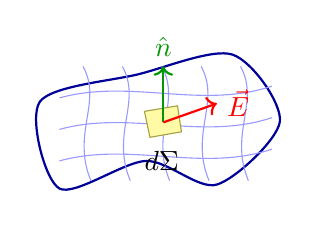
\begin{tikzpicture}[scale=1]
\draw[blue!60!black,thick] plot[smooth cycle] coordinates {(0,0) (1.1,0.35) (2.0,0.05) (2.8,0.85) (2.2,1.7) (1.0,1.45) (-0.25,1.1)};
\foreach \x in {0.4,0.9,1.4,1.9,2.4}{
\draw[blue!40] (\x,0.1) .. controls (\x-0.25,0.7) and (\x+0.15,1.1) .. (\x-0.1,1.55);
}
\foreach \y in {0.35,0.75,1.15}{
\draw[blue!40] (0.0,\y) .. controls (0.9,\y+0.25) and (1.8,\y-0.15) .. (2.7,\y+0.15);
}
\draw[fill=yellow!35,draw=yellow!60!black] (1.15,0.65) -- (1.55,0.72) -- (1.5,1.05) -- (1.08,0.98) -- cycle;
\draw[->,green!60!black,thick] (1.32,0.84) -- (1.32,1.55) node[above] {\(\hat{n}\)};
\draw[->,red,thick] (1.32,0.84) -- (2.0,1.08) node[right] {\(\vec{E}\)};
\node at (1.3,0.35) {\(d\Sigma\)};
\end{tikzpicture}\end{center}

Il flusso infinitesimo attraverso \(d\Sigma\) è
\[
    d\Phi_\Sigma(\vec{E})=\vec{E}\cdot\hat{n}\,d\Sigma.
\]
Il flusso totale si ottiene sommando tutti i contributi infinitesimi, cio integrando sulla superficie:
\[
    \Phi_\Sigma(\vec{E})=
\int_\Sigma \vec{E}\cdot\hat{n}\,d\Sigma.
\]

\begin{snippetdefinition}{Flusso di un campo vettoriale}
Il flusso del campo vettoriale \(\vec{E}\) attraverso una superficie orientata \(\Sigma\) è
\[
    \Phi_\Sigma(\vec{E})=
\int_\Sigma \vec{E}\cdot\hat{n}\,d\Sigma.
\]
Se \(\Sigma\) è chiusa, la normale \(\hat{n}\) si prende per convenzione uscente dalla superficie.
\end{snippetdefinition}

Nel caso del campo elettrico, le dimensioni del flusso sono
\[
    [\Phi_\Sigma(\vec{E})]=[E][\Sigma]
=\frac{\mathrm{N}}{\mathrm{C}}\,\mathrm{m}^2.
\]

\section{Legge di Gauss}

Consideriamo ora una superficie chiusa \(\Sigma\). Il flusso del campo elettrico attraverso \(\Sigma\) è
\[
    \Phi_\Sigma(\vec{E})=
\oint_\Sigma \vec{E}\cdot\hat{n}\,d\Sigma,
\]
dove il simbolo \(\oint\) ricorda che la superficie è chiusa.

\begin{snippettheorem}{Legge di Gauss}
Il flusso del campo elettrico attraverso una superficie chiusa \(\Sigma\) è uguale alla carica totale racchiusa dalla superficie divisa per \(\varepsilon_0\):
\[
    \Phi_\Sigma(\vec{E})=
\oint_\Sigma \vec{E}\cdot\hat{n}\,d\Sigma
=\frac{q_{\mathrm{int}}}{\varepsilon_0}.
\]
\end{snippettheorem}

La carica \(q_{\mathrm{int}}\) è la carica interna alla superficie. Le cariche esterne possono modificare localmente il campo sulla superficie, ma non modificano il flusso netto totale attraverso una superficie chiusa.

\begin{center}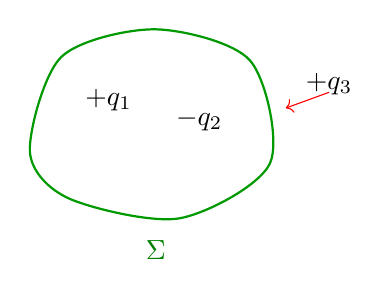
\begin{tikzpicture}[scale=1]
\draw[green!60!black,thick] plot[smooth cycle] coordinates {(-1.6,-0.3) (-1.2,0.9) (0.0,1.25) (1.2,0.85) (1.45,-0.45) (0.3,-1.15) (-1.1,-0.9)};
\node at (-0.6,0.35) {\(+q_1\)};
\node at (0.55,0.1) {\(-q_2\)};
\node at (2.2,0.55) {\(+q_3\)};
\draw[->,red] (2.2,0.45) -- (1.65,0.25);
\node[green!50!black] at (0,-1.55) {\(\Sigma\)};
\end{tikzpicture}\end{center}

Per esempio, nella figura la superficie racchiude \(q_1\) e \(q_2\), mentre \(q_3\) è esterna. Allora
\[
    \Phi_\Sigma(\vec{E})=\frac{q_1+q_2}{\varepsilon_0}.
\]
Se invece una superficie chiusa non racchiude carica netta, il flusso totale è nullo.

\section{Uso pratico della legge di Gauss}

La legge di Gauss è sempre vera, ma è particolarmente utile quando il problema possiede una simmetria sufficiente. In tal caso si può scegliere una superficie chiusa \emph{intelligente}, cioè una superficie sulla quale il campo abbia proprietà semplici.

In pratica si cerca una superficie chiusa \(\Sigma\) tale che:
\begin{itemize}
\item su una parte \(\Sigma_\perp\), il campo sia perpendicolare alla superficie e uniforme;
\item su una parte \(\Sigma_\parallel\), il campo sia parallelo alla superficie, quindi il flusso sia nullo.
\end{itemize}
Allora
\[
    \Sigma=\Sigma_\perp\cup\Sigma_\parallel
\qquad
\Phi_\Sigma(\vec{E})=
\Phi_{\Sigma_\perp}(\vec{E})+\Phi_{\Sigma_\parallel}(\vec{E}).
\]
Sulla parte parallela il flusso è nullo, mentre sulla parte perpendicolare
\[
    \Phi_{\Sigma_\perp}(\vec{E})=E\Sigma_\perp.
\]
Quindi la legge di Gauss diventa
\[
    E\Sigma_\perp=\frac{q_{\mathrm{int}}}{\varepsilon_0},
\qquad
E=\frac{q_{\mathrm{int}}}{\varepsilon_0\Sigma_\perp}.
\]
Questa è spesso la forma operativa pi comoda.

\section{Piano infinito uniformemente carico}

Consideriamo un piano infinito con densità superficiale uniforme di carica \(\sigma\). Per simmetria, il campo elettrico è perpendicolare al piano e ha lo stesso modulo sui due lati.

\begin{center}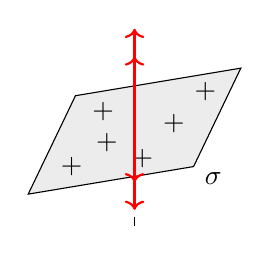
\begin{tikzpicture}[scale=1]
\draw[fill=gray!15,draw=black] (0,0) -- (2.1,0.35) -- (2.7,1.6) -- (0.6,1.25) -- cycle;
\foreach \x/\y in {0.55/0.35,1.0/0.65,1.45/0.45,1.85/0.9,0.95/1.05,2.25/1.3}{
\node at (\x,\y) {\(+\)};
}
\draw[dashed] (1.35,-0.4) -- (1.35,2.0);
\foreach \y in {-0.2,0.15,1.75,2.1}{
\draw[->,red,thick] (1.35,0.8) -- (1.35,\y);
}
\node at (2.35,0.2) {\(\sigma\)};
\end{tikzpicture}\end{center}

Scegliamo come superficie gaussiana un cilindro con asse perpendicolare al piano. Le due basi hanno area \(S\), mentre la superficie laterale è parallela al campo e quindi non contribuisce al flusso.

\begin{center}\begin{tikzpicture}[scale=1]
\draw[fill=gray!15,draw=black] (-1.7,0) -- (1.7,0.25) -- (2.0,1.15) -- (-1.4,0.9) -- cycle;
\draw[blue,thick] (0,0.55) ellipse (0.45 and 0.13);
\draw[blue,thick] (0,-0.75) ellipse (0.45 and 0.13);
\draw[blue,thick] (-0.45,-0.75) -- (-0.45,0.55);
\draw[blue,thick] (0.45,-0.75) -- (0.45,0.55);
\draw[->,red,thick] (0,0.55) -- (0,1.35) node[above] {\(\vec{E}\)};
\draw[->,red,thick] (0,-0.75) -- (0,-1.55) node[below] {\(\vec{E}\)};
\node[blue] at (0.75,-0.1) {\(\Sigma\)};
\end{tikzpicture}\end{center}

La parte utile della superficie è data dalle due basi:
\[
    \Sigma_\perp=2S.
\]
La carica interna è la carica del pezzo di piano contenuto nel cilindro:
\[
    q_{\mathrm{int}}=\sigma S.
\]
La legge di Gauss dà
\[
    E(2S)=\frac{\sigma S}{\varepsilon_0}.
\]
Quindi
\[
    E=\frac{\sigma}{2\varepsilon_0}.
\]

\begin{snippettheorem}{Campo elettrico di un piano infinito carico}
Il campo elettrico generato da un piano infinito uniformemente carico con densità superficiale \(\sigma\) ha modulo
\[
    E=\frac{\sigma}{2\varepsilon_0}.
\]
Il campo è perpendicolare al piano, uscente se \(\sigma>0\) ed entrante se \(\sigma<0\).
\end{snippettheorem}

Il risultato non dipende dalla dimensione del cilindro gaussiano scelto. Questo accade perché la carica racchiusa cresce come l'area della base, e il flusso cresce anch'esso come la stessa area.

\section{Carica puntiforme e simmetria sferica}

Consideriamo una carica puntiforme \(q\). Il campo elettrico deve essere radiale e dipendere solo dalla distanza \(r\) dalla carica. Per sfruttare la simmetria scegliamo come superficie gaussiana una sfera centrata sulla carica.

\begin{center}\begin{tikzpicture}[scale=1]
\fill (0,0) circle (1.5pt) node[below] {\(q\)};
\foreach \a in {0,30,...,330}{
\draw[->,red] ({0.25*cos(\a)},{0.25*sin(\a)}) -- ({1.15*cos(\a)},{1.15*sin(\a)});
}
\draw[blue,thick] (0,0) circle (1.25);
\draw[->,green!60!black] (0,0) -- (1.25,0) node[midway,below] {\(r\)};
\node[blue] at (1.55,0.55) {\(\Sigma\)};
\end{tikzpicture}\end{center}

Sulla sfera il campo è perpendicolare alla superficie e ha modulo costante. Non c'è una parte \(\Sigma_\parallel\), quindi
\[
    \Sigma_\perp=4\pi r^2.
\]
La carica racchiusa è
\[
    q_{\mathrm{int}}=q.
\]
Per la legge di Gauss,
\[
    E4\pi r^2=\frac{q}{\varepsilon_0},
\]
da cui
\[
    E=\frac{q}{4\pi\varepsilon_0r^2}.
\]

\begin{snippettheorem}{Campo elettrico di una carica puntiforme}
Il campo elettrico generato da una carica puntiforme \(q\) è
\[
    \vec{E}(r)=\frac{q}{4\pi\varepsilon_0r^2}\hat{r}.
\]
Questa è la stessa legge ottenuta dalla legge di Coulomb.
\end{snippettheorem}

Infatti, dalla legge di Coulomb, la forza su una carica di prova \(q_0\) sarebbe
\[
    F=\frac{1}{4\pi\varepsilon_0}\frac{qq_0}{r^2}.
\]
Dividendo per \(q_0\), si ottiene
\[
    E=\frac{F}{q_0}=\frac{q}{4\pi\varepsilon_0r^2}.
\]

\section{Guscio sferico carico}

Consideriamo un guscio sferico di raggio \(R\), uniformemente carico con carica totale \(q\). Per simmetria il campo elettrico è radiale. Distinguiamo due regioni.

\subsection{Interno del guscio}

Se \(r<R\), scegliamo una superficie gaussiana sferica di raggio \(r\) interna al guscio. Essa non racchiude alcuna carica:
\[
    q_{\mathrm{int}}=0.
\]
Per la legge di Gauss,
\[
    E4\pi r^2=0,
\]
quindi
\[
    E=0\qquad r<R.
\]

\subsection{Esterno del guscio}

Se \(r>R\), la superficie gaussiana sferica racchiude tutta la carica \(q\). Allora
\[
    E4\pi r^2=\frac{q}{\varepsilon_0},
\]
e quindi
\[
    E=\frac{q}{4\pi\varepsilon_0r^2}\qquad r>R.
\]

\begin{snippettheorem}{Campo elettrico di un guscio sferico uniforme}
Per un guscio sferico uniformemente carico di raggio \(R\) e carica totale \(q\), il campo elettrico è
\[
    E(r)=
\begin{cases}
0, & r<R,\\[4pt]
\displaystyle \frac{q}{4\pi\varepsilon_0r^2}, & r>R.
\end{cases}
\]
All'esterno il guscio si comporta come una carica puntiforme posta nel centro; all'interno il campo è nullo.
\end{snippettheorem}

\begin{center}\begin{tikzpicture}[scale=1]
\draw[->] (0,0) -- (5.0,0) node[right] {\(r\)};
\draw[->] (0,0) -- (0,2.4) node[above] {\(E(r)\)};
\draw[red,thick] (0,0) -- (2,0);
\draw[red,thick,domain=2:4.7,samples=100] plot (\x,{8/(\x*\x)});
\draw[dashed] (2,0) -- (2,2);
\draw[dashed] (0,2) -- (2,2);
\node[below] at (2,0) {\(R\)};
\node[left] at (0,2) {\(\frac{q}{4\pi\varepsilon_0R^2}\)};
\node at (3.7,0.8) {\(\sim r^{-2}\)};
\end{tikzpicture}\end{center}

\section{Potenziale del guscio sferico}

Scegliamo il potenziale nullo all'infinito:
\[
    V(\infty)=0.
\]
Per \(r>R\), il campo è quello di una carica puntiforme, quindi
\[
    V(r)=\frac{q}{4\pi\varepsilon_0r}.
\]
Per \(r<R\), invece, il campo è nullo. Quindi il potenziale è costante all'interno del guscio:
\[
    E=0\qquad\Longrightarrow\qquad V=\text{costante}.
\]
La costante si trova imponendo la continuità del potenziale in \(r=R\). Poiché
\[
    V(R)=\frac{q}{4\pi\varepsilon_0R},
\]
si ha
\[
    V(r)=\frac{q}{4\pi\varepsilon_0R}
\qquad r<R.
\]

\begin{snippettheorem}{Potenziale del guscio sferico}
Per un guscio sferico uniformemente carico, con \(V(\infty)=0\), il potenziale è
\[
    V(r)=
\begin{cases}
\displaystyle \frac{q}{4\pi\varepsilon_0R}, & r<R,\\[6pt]
\displaystyle \frac{q}{4\pi\varepsilon_0r}, & r>R.
\end{cases}
\]
\end{snippettheorem}

\begin{center}\begin{tikzpicture}[scale=1]
\draw[->] (0,0) -- (5.0,0) node[right] {\(r\)};
\draw[->] (0,0) -- (0,2.4) node[above] {\(V(r)\)};
\draw[red,thick] (0,1.8) -- (2,1.8);
\draw[red,thick,domain=2:4.7,samples=100] plot (\x,{3.6/\x});
\draw[dashed] (2,0) -- (2,1.8);
\node[below] at (2,0) {\(R\)};
\node[left] at (0,1.8) {\(\frac{q}{4\pi\varepsilon_0R}\)};
\node at (3.6,0.8) {\(\sim r^{-1}\)};
\end{tikzpicture}\end{center}

Il limite del campo per \(r\to R^+\) è
\[
    E(R^+)=\frac{q}{4\pi\varepsilon_0R^2},
\]
mentre il limite per \(r\to R^-\) è
\[
    E(R^-)=0.
\]
Quindi il campo presenta un salto sulla superficie del guscio. Il potenziale, invece, resta continuo.


\pagebreak
\part{Lezione 8}

\section{Richiamo: legge di Gauss}

La legge di Gauss afferma che il flusso del campo elettrico attraverso una superficie chiusa \(\Sigma\) è uguale alla carica totale racchiusa divisa per \(\varepsilon_0\):
\[
    \Phi_\Sigma(\vec{E})=
\oint_\Sigma \vec{E}\cdot\hat{n}\,d\Sigma
=\frac{q_{\mathrm{int}}}{\varepsilon_0}.
\]
Qui \(\hat{n}\) è il versore normale uscente dalla superficie.

Quando per simmetria il campo è uniforme su una parte \(\Sigma_\perp\) della superficie ed è perpendicolare ad essa, mentre sulle altre parti il flusso è nullo, la legge di Gauss si riduce a
\[
    E\Sigma_\perp=\frac{q_{\mathrm{int}}}{\varepsilon_0},
\qquad
E=\frac{q_{\mathrm{int}}}{\varepsilon_0\Sigma_\perp}.
\]
Questa forma è molto utile per calcolare campi elettrici in presenza di simmetria.

\section{Sfera uniformemente carica}

Consideriamo una sfera piena di raggio \(R\), uniformemente carica con carica totale \(q\). La densità volumica di carica è costante e vale
\[
    \rho=\frac{q}{\frac{4}{3}\pi R^3}.
\]
Per simmetria il campo elettrico è radiale e dipende solo dalla distanza \(r\) dal centro:
\[
    \vec{E}(r)=E(r)\hat{r}.
\]

\begin{center}\begin{tikzpicture}[scale=1]
\draw[fill=gray!15,draw=black] (0,0) circle (1.2);
\foreach \x/\y in {-0.5/0.6,0.2/0.4,0.55/-0.25,-0.35/-0.35,0.0/0.85,0.65/0.65}{
\node at (\x,\y) {\(+\)};
}
\draw[->,green!60!black,thick] (0,0) -- (1.2,0) node[midway,below] {\(R\)};
\draw[->,red,thick] (1.35,0.25) -- (2.0,0.45) node[right] {\(\vec{E}\)};
\node at (0,-1.55) {sfera piena uniformemente carica};
\end{tikzpicture}\end{center}

\subsection{Campo esterno alla sfera}

Se \(r>R\), scegliamo come superficie gaussiana una sfera di raggio \(r\) concentrica con la distribuzione. Su questa superficie il campo è costante in modulo e parallelo alla normale uscente. Dunque
\[
    \oint_\Sigma \vec{E}\cdot\hat{n}\,d\Sigma=E(r)4\pi r^2.
\]
La carica racchiusa è tutta la carica della sfera:
\[
    q_{\mathrm{int}}=q.
\]
Per la legge di Gauss,
\[
    E(r)4\pi r^2=\frac{q}{\varepsilon_0},
\]
e quindi
\[
    E(r)=\frac{q}{4\pi\varepsilon_0r^2}\qquad r>R.
\]

\begin{snippetproposition}{Campo esterno di una sfera uniformemente carica}
All'esterno di una sfera uniformemente carica, il campo elettrico è uguale a quello di una carica puntiforme \(q\) posta nel centro:
\[
    \vec{E}(r)=\frac{q}{4\pi\varepsilon_0r^2}\hat{r}
\qquad r>R.
\]
\end{snippetproposition}

\subsection{Campo interno alla sfera}

Se \(r<R\), scegliamo come superficie gaussiana una sfera concentrica di raggio \(r\). In questo caso la superficie racchiude solo la carica contenuta nella sfera di raggio \(r\). Poiché la densità è uniforme,
\[
    q_{\mathrm{int}}=\rho\frac{4}{3}\pi r^3.
\]
Sostituendo \(\rho=q/(\frac{4}{3}\pi R^3)\), otteniamo
\[
    q_{\mathrm{int}}=q\frac{r^3}{R^3}.
\]
La legge di Gauss dà
\[
    E(r)4\pi r^2=\frac{1}{\varepsilon_0}q\frac{r^3}{R^3}.
\]
Quindi
\[
    E(r)=\frac{q}{4\pi\varepsilon_0R^3}r
\qquad r<R.
\]

\begin{snippetproposition}{Campo interno di una sfera uniformemente carica}
All'interno di una sfera piena uniformemente carica il campo elettrico cresce linearmente con la distanza dal centro:
\[
    \vec{E}(r)=\frac{q}{4\pi\varepsilon_0R^3}r\hat{r}
\qquad r<R.
\]
\end{snippetproposition}

Riassumendo,
\[
    E(r)=
\begin{cases}
\displaystyle \frac{q}{4\pi\varepsilon_0R^3}r, & r<R,\\[6pt]
\displaystyle \frac{q}{4\pi\varepsilon_0r^2}, & r>R.
\end{cases}
\]
Il campo è continuo in \(r=R\), perché entrambi i valori danno
\[
    E(R)=\frac{q}{4\pi\varepsilon_0R^2}.
\]

\begin{center}\begin{tikzpicture}[scale=1]
\draw[->] (0,0) -- (5.2,0) node[right] {\(r\)};
\draw[->] (0,0) -- (0,2.6) node[above] {\(E(r)\)};
\draw[red,thick] (0,0) -- (2,2);
\draw[red,thick,domain=2:4.8,samples=100] plot (\x,{8/(\x*\x)});
\draw[dashed] (2,0) -- (2,2);
\draw[dashed] (0,2) -- (2,2);
\node[below] at (2,0) {\(R\)};
\node[left] at (0,2) {\(\frac{q}{4\pi\varepsilon_0R^2}\)};
\node at (1.05,1.45) {\(\sim r\)};
\node at (3.7,0.8) {\(\sim r^{-2}\)};
\end{tikzpicture}\end{center}

\section{Potenziale di una sfera uniformemente carica}

Scegliamo il potenziale nullo all'infinito:
\[
    V(\infty)=0.
\]
Per \(r>R\), il campo è quello di una carica puntiforme, quindi
\[
    V(r)=\frac{q}{4\pi\varepsilon_0r}
\qquad r>R.
\]

Per \(r<R\), usiamo la relazione lungo una linea radiale:
\[
    E(r)=-\frac{dV}{dr}.
\]
Poiché
\[
    E(r)=\frac{q}{4\pi\varepsilon_0R^3}r,
\]
si ha
\[
    \frac{dV}{dr}=-\frac{q}{4\pi\varepsilon_0R^3}r.
\]
Integrando,
\[
    V(r)=-\frac{q}{4\pi\varepsilon_0R^3}\frac{r^2}{2}+C.
\]
La costante si determina imponendo la continuità del potenziale in \(r=R\). Dall'esterno,
\[
    V(R)=\frac{q}{4\pi\varepsilon_0R}.
\]
Dall'interno,
\[
    V(R)=-\frac{q}{4\pi\varepsilon_0R^3}\frac{R^2}{2}+C.
\]
Quindi
\[
    \frac{q}{4\pi\varepsilon_0R}
=-\frac{q}{8\pi\varepsilon_0R}+C,
\]
da cui
\[
    C=\frac{3}{2}\frac{q}{4\pi\varepsilon_0R}.
\]
Pertanto
\[
    V(r)=\frac{q}{4\pi\varepsilon_0R}\frac{1}{2}\left(3-\frac{r^2}{R^2}\right)
\qquad r<R.
\]

\begin{snippettheorem}{Potenziale di una sfera uniformemente carica}
Per una sfera piena uniformemente carica di raggio \(R\), con \(V(\infty)=0\), il potenziale è
\[
    V(r)=
\begin{cases}
\displaystyle \frac{q}{4\pi\varepsilon_0R}\frac{1}{2}\left(3-\frac{r^2}{R^2}\right), & r<R,\\[8pt]
\displaystyle \frac{q}{4\pi\varepsilon_0r}, & r>R.
\end{cases}
\]
In particolare,
\[
    V(0)=\frac{3}{2}\frac{q}{4\pi\varepsilon_0R},
\qquad
V(R)=\frac{q}{4\pi\varepsilon_0R}.
\]
\end{snippettheorem}

\begin{center}\begin{tikzpicture}[scale=1]
\draw[->] (0,0) -- (5.2,0) node[right] {\(r\)};
\draw[->] (0,0) -- (0,2.8) node[above] {\(V(r)\)};
\draw[red,thick,domain=0:2,samples=100] plot (\x,{2.4-0.4*\x*\x});
\draw[red,thick,domain=2:4.8,samples=100] plot (\x,{4/\x});
\draw[dashed] (2,0) -- (2,1.98);
\draw[dashed] (0,2.4) -- (2,2.4);
\draw[dashed] (0,2.0) -- (2,2.0);
\node[below] at (2,0) {\(R\)};
\node[left] at (0,2.4) {\(\frac{3}{2}\frac{q}{4\pi\varepsilon_0R}\)};
\node[left] at (0,2.0) {\(\frac{q}{4\pi\varepsilon_0R}\)};
\node at (1.0,1.55) {\(\sim -r^2\)};
\node at (3.7,0.8) {\(\sim r^{-1}\)};
\end{tikzpicture}\end{center}

\section{Simmetria cilindrica: filo infinito carico}

Consideriamo un filo infinito con densità lineare di carica uniforme \(\lambda\). Per simmetria, il campo elettrico è radiale rispetto al filo e il suo modulo dipende solo dalla distanza \(r\) dal filo.

\begin{center}\begin{tikzpicture}[scale=1]
\draw[dashed] (0,-1.4) -- (0,1.8);
\draw[->,red,thick] (0,0) -- (1.2,0) node[midway,below] {\(\vec{E}\)};
\draw[->,red,thick] (0,0) -- (-1.0,0.7);
\draw[->,red,thick] (0,0) -- (-1.0,-0.7);
\node at (-0.25,1.55) {filo};
\node at (0.55,0.2) {\(r\)};
\end{tikzpicture}\end{center}

Scegliamo come superficie gaussiana un cilindro coassiale al filo, di raggio \(r\) e altezza \(h\). Il flusso attraverso le basi è nullo, perché il campo è parallelo alle basi. Il flusso attraversa solo la superficie laterale, di area
\[
    \Sigma_{\mathrm{lat}}=2\pi rh.
\]
La carica racchiusa è
\[
    q_{\mathrm{int}}=\lambda h.
\]
La legge di Gauss diventa
\[
    E(r)2\pi rh=\frac{\lambda h}{\varepsilon_0}.
\]
Quindi
\[
    E(r)=\frac{\lambda}{2\pi\varepsilon_0r}.
\]

\begin{snippettheorem}{Campo elettrico di un filo infinito}
Il campo elettrico generato da un filo infinito con densità lineare uniforme \(\lambda\) è
\[
    \vec{E}(r)=\frac{\lambda}{2\pi\varepsilon_0r}\hat{r}.
\]
Il modulo decresce come \(1/r\).
\end{snippettheorem}

\begin{center}\begin{tikzpicture}[scale=1]
\draw (0,0) ellipse (0.55 and 0.18);
\draw (-0.55,0) -- (-0.55,2.0);
\draw (0.55,0) -- (0.55,2.0);
\draw (0,2.0) ellipse (0.55 and 0.18);
\draw[dashed] (0,-0.2) -- (0,2.25);
\draw[->,red,thick] (0.55,1.0) -- (1.35,1.0) node[right] {\(\vec{E}\)};
\draw[<->] (0,-0.45) -- (0.55,-0.45) node[midway,below] {\(r\)};
\draw[<->] (-0.85,0) -- (-0.85,2.0) node[midway,left] {\(h\)};
\node at (0,-0.85) {superficie gaussiana cilindrica};
\end{tikzpicture}\end{center}

\subsection{Potenziale del filo infinito}

Lungo una direzione radiale,
\[
    E(r)=-\frac{dV}{dr}.
\]
Poiché
\[
    E(r)=\frac{\lambda}{2\pi\varepsilon_0r},
\]
si ottiene
\[
    V(r)=-\frac{\lambda}{2\pi\varepsilon_0}\ln r+C.
\]
In questo caso non si può imporre \(V(\infty)=0\), perché \(\ln r\) diverge per \(r\to\infty\). Si sceglie quindi un raggio di riferimento \(r_0\) e si pone \(V(r_0)=0\). Allora
\[
    V(r)=\frac{\lambda}{2\pi\varepsilon_0}\ln\left(\frac{r_0}{r}\right).
\]

\begin{snippetproposition}{Potenziale del filo infinito}
Il potenziale del filo infinito è definito solo rispetto a un raggio di riferimento finito \(r_0\). Con la scelta \(V(r_0)=0\), vale
\[
    V(r)=\frac{\lambda}{2\pi\varepsilon_0}\ln\left(\frac{r_0}{r}\right).
\]
Non si può scegliere il potenziale nullo all'infinito.
\end{snippetproposition}

\section{Riepilogo delle simmetrie principali}

\begin{snippetproposition}{Distribuzioni con simmetria sferica}
Per una distribuzione di carica a simmetria sferica, all'esterno della distribuzione il campo elettrico si comporta come quello di una carica puntiforme posta nel centro:
\[
    E(r)\sim \frac{1}{r^2}.
\]
Esempi sono il guscio sferico carico e la sfera uniformemente carica.
\end{snippetproposition}

\begin{snippetproposition}{Distribuzioni con simmetria cilindrica}
Per una distribuzione infinita a simmetria cilindrica, come un filo infinito uniformemente carico, si usa una superficie gaussiana cilindrica. Il campo elettrico del filo infinito è
\[
    E(r)=\frac{\lambda}{2\pi\varepsilon_0r},
\]
quindi
\[
    E(r)\sim \frac{1}{r}.
\]
\end{snippetproposition}

\begin{snippetproposition}{Distribuzioni con simmetria piana}
Per un piano infinito uniformemente carico, il campo elettrico ha modulo
\[
    E=\frac{\sigma}{2\varepsilon_0}.
\]
Il campo non dipende dalla distanza dal piano e non tende a zero all'infinito, perché la distribuzione è idealmente infinita.
\end{snippetproposition}

\begin{center}\begin{tikzpicture}[scale=1]
\draw[->] (0,0) -- (2.1,0) node[right] {\(r\)};
\draw[->] (0,0) -- (0,1.7) node[above] {\(E\)};
\draw[red,thick,domain=0.35:2,samples=80] plot (\x,{0.7/(\x*\x)});
\node at (1.0,-0.45) {sferica};
\draw[->] (3,0) -- (5.1,0) node[right] {\(r\)};
\draw[->] (3,0) -- (3,1.7) node[above] {\(E\)};
\draw[red,thick,domain=3.35:5,samples=80] plot (\x,{0.75/(\x-3)});
\node at (4.0,-0.45) {cilindrica};
\draw[->] (6,0) -- (8.1,0) node[right] {\(r\)};
\draw[->] (6,0) -- (6,1.7) node[above] {\(E\)};
\draw[red,thick] (6.25,1.05) -- (8.0,1.05);
\node at (7.0,-0.45) {piana};
\end{tikzpicture}\end{center}

\section{Legge di Gauss in forma differenziale}

La legge di Gauss in forma integrale è
\[
    \oint_\Sigma \vec{E}\cdot\hat{n}\,d\Sigma
=\frac{q_{\mathrm{int}}}{\varepsilon_0}.
\]
Questa forma è globale: mette in relazione il flusso su una superficie chiusa con la carica totale interna. Vogliamo ora ricavare una forma locale, valida punto per punto.

\begin{snippettheorem}{Teorema della divergenza}
Sia \(\vec{A}\) un campo vettoriale differenziabile con continuità in un volume \(\Omega\), e sia \(\Sigma=\partial\Omega\) la sua superficie chiusa orientata verso l'esterno. Allora
\[
    \oint_\Sigma \vec{A}\cdot\hat{n}\,d\Sigma
=\int_\Omega \vec{\nabla}\cdot\vec{A}\,d\Omega.
\]
In coordinate cartesiane,
\[
    \vec{\nabla}\cdot\vec{A}=\frac{\partial A_x}{\partial x}+\frac{\partial A_y}{\partial y}+\frac{\partial A_z}{\partial z}.
\]
\end{snippettheorem}

Applicando il teorema della divergenza al campo elettrico,
\[
    \oint_\Sigma \vec{E}\cdot\hat{n}\,d\Sigma
=\int_\Omega \vec{\nabla}\cdot\vec{E}\,d\Omega.
\]
La carica interna può essere scritta come integrale della densità volumica di carica:
\[
    q_{\mathrm{int}}=\int_\Omega \rho\,d\Omega.
\]
La legge di Gauss diventa quindi
\[
    \int_\Omega \vec{\nabla}\cdot\vec{E}\,d\Omega
=\frac{1}{\varepsilon_0}\int_\Omega \rho\,d\Omega.
\]
Portando tutto al primo membro,
\[
    \int_\Omega \left(\vec{\nabla}\cdot\vec{E}-\frac{\rho}{\varepsilon_0}\right)d\Omega=0.
\]
Poiché questa uguaglianza vale per ogni volume \(\Omega\), l'integrando deve essere nullo punto per punto:
\[
    \vec{\nabla}\cdot\vec{E}=\frac{\rho}{\varepsilon_0}.
\]

\begin{snippettheorem}{Legge di Gauss in forma differenziale}
La forma differenziale della legge di Gauss è
\[
    \vec{\nabla}\cdot\vec{E}=\frac{\rho}{\varepsilon_0}.
\]
Essa esprime localmente il legame tra la divergenza del campo elettrico e la densità di carica.
\end{snippettheorem}

\section{Leggi dell'elettrostatica in forma differenziale}

In elettrostatica il campo elettrico è conservativo. Esiste dunque un potenziale \(V\) tale che
\[
    \vec{E}=-\vec{\nabla}V.
\]
Equivalentemente, il rotore del campo elettrico è nullo:
\[
    \vec{\nabla}\times\vec{E}=\vec{0}.
\]

\begin{snippettheorem}{Equazioni fondamentali dell'elettrostatica}
Le due equazioni locali dell'elettrostatica sono
\[
    \vec{\nabla}\times\vec{E}=\vec{0},
\qquad
\vec{\nabla}\cdot\vec{E}=\frac{\rho}{\varepsilon_0}.
\]
La prima esprime la conservatività del campo elettrico; la seconda è la legge di Gauss in forma differenziale.
\end{snippettheorem}

\section{Conduttori e isolanti}

In un conduttore esistono cariche libere che possono muoversi. Nei metalli queste cariche sono gli elettroni di conduzione. In un isolante, invece, le cariche non possono muoversi liberamente su distanze macroscopiche.

\begin{snippetdefinition}{Conduttore e isolante}
Un conduttore è un materiale in cui alcune cariche sono libere di muoversi. Un isolante è un materiale in cui le cariche non possono muoversi liberamente su scala macroscopica.
\end{snippetdefinition}

Se aggiungiamo carica a una sfera metallica, le cariche libere si respingono e si distribuiscono sulla superficie. Se invece aggiungiamo carica a una sfera isolante, la carica resta sostanzialmente nella regione in cui viene depositata.

\begin{center}\begin{tikzpicture}[scale=1]
\draw[fill=gray!20,draw=black] (0,0) circle (0.9);
\foreach \a in {20,70,120,170,220,270,320}{
\node at ({0.92*cos(\a)},{0.92*sin(\a)}) {\scriptsize \(+\)};
}
\node at (0,-1.25) {sfera metallica};
\draw[fill=gray!20,draw=black] (3,0) circle (0.9);
\foreach \x/\y in {2.75/0.2,3.15/0.4,3.0/-0.25,3.35/-0.05}{
\node at (\x,\y) {\scriptsize \(+\)};
}
\node at (3,-1.25) {sfera isolante};
\end{tikzpicture}\end{center}

\section{Conduttore in equilibrio elettrostatico}

In equilibrio elettrostatico le cariche libere di un conduttore sono ferme. Se all'interno del conduttore ci fosse un campo elettrico non nullo, le cariche subirebbero una forza
\[
    \vec{F}=q\vec{E}
\]
e si muoverebbero. Dunque, in equilibrio, deve valere
\[
    \vec{E}=\vec{0}
\]
in ogni punto interno del conduttore.

\begin{snippettheorem}{Campo interno di un conduttore in equilibrio}
In un conduttore in equilibrio elettrostatico il campo elettrico interno è nullo:
\[
    \vec{E}=\vec{0}.
\]
\end{snippettheorem}

Da questa proprietà seguono tre conseguenze fondamentali.

\subsection{Prima conseguenza: la carica si distribuisce sulla superficie}

Consideriamo una superficie chiusa \(\Sigma\) interamente contenuta all'interno del conduttore. Poiché \(\vec{E}=\vec{0}\) su \(\Sigma\), il flusso è nullo:
\[
    \Phi_\Sigma(\vec{E})=0.
\]
Per la legge di Gauss,
\[
    0=\frac{q_{\mathrm{int}}}{\varepsilon_0}.
\]
Dunque
\[
    q_{\mathrm{int}}=0.
\]
Quindi non può esserci carica netta nel volume interno del conduttore: l'eventuale carica in eccesso si dispone sulla superficie.

\begin{snippetproposition}{Carica in un conduttore}
In un conduttore in equilibrio elettrostatico, la carica in eccesso si distribuisce sulla superficie esterna del conduttore.
\end{snippetproposition}

\begin{center}\begin{tikzpicture}[scale=1]
\draw[fill=gray!20,draw=black] plot[smooth cycle] coordinates {(-1.4,-0.5) (-1.1,0.8) (0.1,1.1) (1.2,0.55) (1.1,-0.8) (-0.3,-1.1)};
\foreach \x/\y in {-1.05/0.45,-0.45/0.95,0.45/0.9,1.05/0.2,0.7/-0.75,-0.45/-0.95,-1.15/-0.2}{
\node at (\x,\y) {\scriptsize \(+\)};
}
\draw[blue,thick] (0,0) ellipse (0.55 and 0.35);
\node[blue] at (0.15,0.5) {\(\Sigma\)};
\node at (0,0) {\(E=0\)};
\end{tikzpicture}\end{center}

\subsection{Seconda conseguenza: il conduttore è equipotenziale}

Siano \(P_1\) e \(P_2\) due punti qualsiasi del conduttore, anche sulla superficie. Poiché dentro il conduttore \(\vec{E}=\vec{0}\), si ha
\[
    V(P_2)-V(P_1)=-\int_{P_1}^{P_2}\vec{E}\cdot d\vec{s}=0.
\]
Quindi
\[
    V(P_1)=V(P_2).
\]

\begin{snippetproposition}{Conduttore equipotenziale}
In equilibrio elettrostatico il potenziale è costante in tutto il conduttore, compresa la superficie.
\end{snippetproposition}

\subsection{Terza conseguenza: campo esterno perpendicolare alla superficie}

La superficie di un conduttore in equilibrio è una superficie equipotenziale. Il campo elettrico è perpendicolare alle superfici equipotenziali. Quindi, appena fuori dal conduttore, il campo non può avere componente tangenziale.

Se esistesse una componente tangenziale del campo, le cariche libere sulla superficie subirebbero una forza lungo la superficie e si muoverebbero. Questo contraddirebbe l'equilibrio elettrostatico.

\begin{snippetproposition}{Direzione del campo sulla superficie di un conduttore}
Il campo elettrico immediatamente all'esterno di un conduttore in equilibrio elettrostatico è perpendicolare alla superficie:
\[
    \vec{E}_{\mathrm{est}}\parallel \hat{n}.
\]
\end{snippetproposition}

\begin{center}\begin{tikzpicture}[scale=1]
\draw[fill=gray!20,draw=black] plot[smooth cycle] coordinates {(-1.2,-0.55) (-0.9,0.65) (0.1,0.95) (1.1,0.4) (0.8,-0.75) (-0.25,-0.9)};
\draw[->,red,thick] (0.55,0.82) -- (0.75,1.55) node[above] {\(\vec{E}\)};
\draw[dashed] (-0.05,0.9) .. controls (0.4,1.0) and (0.75,0.85) .. (1.05,0.55);
\node at (0,-1.25) {\(\vec{E}\perp\) superficie};
\end{tikzpicture}\end{center}

\section{Teorema di Coulomb}

Vogliamo determinare il modulo del campo elettrico appena all'esterno di un conduttore in equilibrio. Consideriamo un piccolo cilindro gaussiano, detto anche pillbox, che attraversa la superficie del conduttore. La base superiore è appena fuori dal conduttore, la base inferiore è appena dentro il conduttore.

\begin{center}\begin{tikzpicture}[scale=1]
\draw[thick] (-2.0,0) .. controls (-0.9,0.35) and (0.9,0.35) .. (2.0,0);
\fill[gray!20] (-2.0,-0.08) .. controls (-0.9,0.27) and (0.9,0.27) .. (2.0,-0.08) -- (2.0,-0.9) -- (-2.0,-0.9) -- cycle;
\draw (0.05,0.15) ellipse (0.25 and 0.08);
\draw (-0.2,-0.15) -- (-0.2,0.15);
\draw (0.3,-0.15) -- (0.3,0.15);
\draw (0.05,-0.15) ellipse (0.25 and 0.08);
\draw[->,red,thick] (0.05,0.2) -- (0.05,0.95) node[above] {\(\vec{E}\)};
\node at (1.45,-0.45) {conduttore};
\node at (0.65,0.35) {\(S\)};
\node at (-0.75,-0.45) {\(E=0\)};
\end{tikzpicture}\end{center}

Il flusso attraverso il cilindro è la somma di tre contributi:
\[
    \Phi_\Sigma(\vec{E})=
\int_{\Sigma_{\mathrm{sup}}}\vec{E}\cdot\hat{n}\,d\Sigma+
\int_{\Sigma_{\mathrm{inf}}}\vec{E}\cdot\hat{n}\,d\Sigma+
\int_{\Sigma_{\mathrm{lat}}}\vec{E}\cdot\hat{n}\,d\Sigma.
\]
La base inferiore è dentro il conduttore, quindi \(\vec{E}=\vec{0}\) e il suo contributo è nullo. Sulla superficie laterale, nel limite in cui il cilindro è molto basso, il campo è tangente alla superficie laterale e il contributo è nullo. Resta solo la base superiore:
\[
    \Phi_\Sigma(\vec{E})=ES.
\]
La carica racchiusa nel cilindro è quella sulla porzione di superficie attraversata:
\[
    q_{\mathrm{int}}=\sigma S.
\]
Per la legge di Gauss,
\[
    ES=\frac{\sigma S}{\varepsilon_0}.
\]
Pertanto
\[
    E=\frac{\sigma}{\varepsilon_0}.
\]
In forma vettoriale,
\[
    \vec{E}_{\mathrm{est}}=\frac{\sigma}{\varepsilon_0}\hat{n}.
\]

\begin{snippettheorem}{Teorema di Coulomb}
In un conduttore in equilibrio elettrostatico, il campo elettrico appena all'esterno della superficie è
\[
    \vec{E}_{\mathrm{est}}=\frac{\sigma}{\varepsilon_0}\hat{n},
\]
dove \(\sigma\) è la densità superficiale di carica e \(\hat{n}\) è la normale uscente. All'interno del conduttore il campo è nullo.
\end{snippettheorem}


\pagebreak
\part{Lezione 9}

\section{Teorema di Coulomb}

Consideriamo un conduttore in equilibrio elettrostatico. All'interno del conduttore il campo elettrico è nullo:
\[
    \vec{E}=\vec{0}.
\]
La carica in eccesso si dispone sulla superficie esterna del conduttore. Se \(\sigma\) è la densità superficiale di carica in un punto della superficie, il campo elettrico appena all'esterno del conduttore è perpendicolare alla superficie e vale
\[
    \vec{E}=\frac{\sigma}{\varepsilon_0}\hat{n},
\]
dove \(\hat{n}\) è il versore normale uscente dalla superficie.

\begin{snippettheorem}{Teorema di Coulomb}
In un conduttore in equilibrio elettrostatico, il campo elettrico immediatamente all'esterno della superficie è
\[
    \vec{E}_{\mathrm{est}}=\frac{\sigma}{\varepsilon_0}\hat{n}.
\]
Il campo è perpendicolare alla superficie del conduttore.
\end{snippettheorem}

La componente normale del campo presenta quindi un salto attraversando la superficie carica. Infatti all'interno del conduttore il campo è nullo, mentre all'esterno vale \(\sigma/\varepsilon_0\). Perciò
\[
    \Delta E_n=E_{\mathrm{est}}-E_{\mathrm{int}}=\frac{\sigma}{\varepsilon_0}.
\]

\begin{snippetcorollary}{Salto del campo elettrico attraverso una superficie conduttrice}
Attraversando la superficie di un conduttore carico, la componente normale del campo elettrico cambia di
\[
    \Delta E_n=\frac{\sigma}{\varepsilon_0}.
\]
\end{snippetcorollary}

\section{Esempi di applicazione del teorema di Coulomb}

\subsection{Piano infinito carico}

Un piano infinito con densità superficiale di carica \(\sigma\) genera un campo elettrico uniforme su ciascun lato. Per simmetria il campo è perpendicolare al piano e ha modulo
\[
    E=\frac{\sigma}{2\varepsilon_0}.
\]

\begin{center}\begin{tikzpicture}[scale=1]
\draw[thick] (0,-1.3) -- (0,1.3);
\foreach \y in {-1.0,-0.5,0,0.5,1.0}{
\node at (-0.15,\y) {\(+\)};
\draw[->,red,thick] (0.15,\y) -- (1.15,\y);
\draw[->,red,thick] (-0.15,\y) -- (-1.15,\y);
}
\draw[->] (-1.4,-1.5) -- (1.4,-1.5) node[right] {\(x\)};
\node[red] at (0.9,1.45) {\(E=\frac{\sigma}{2\varepsilon_0}\)};
\node[red] at (-1.0,1.45) {\(E=\frac{\sigma}{2\varepsilon_0}\)};
\end{tikzpicture}\end{center}

Il salto della componente normale del campo è
\[
    \Delta E_n=\frac{\sigma}{2\varepsilon_0}-\left(-\frac{\sigma}{2\varepsilon_0}\right)=\frac{\sigma}{\varepsilon_0},
\]
in accordo con il teorema di Coulomb.

\subsection{Sfera conduttrice carica}

Consideriamo una sfera conduttrice isolata, di raggio \(R\), con carica totale \(q\). Per simmetria la carica si distribuisce uniformemente sulla superficie, quindi
\[
    \sigma=\frac{q}{4\pi R^2}.
\]
All'interno della sfera il campo è nullo. All'esterno il campo è lo stesso di una carica puntiforme \(q\) posta nel centro:
\[
    E(r)=\frac{q}{4\pi\varepsilon_0r^2}\qquad r\geq R.
\]
Alla superficie:
\[
    E(R)=\frac{q}{4\pi\varepsilon_0R^2}.
\]
Poiché \(\sigma=q/(4\pi R^2)\), segue
\[
    E(R)=\frac{\sigma}{\varepsilon_0}.
\]

\begin{center}\begin{tikzpicture}[scale=1]
\draw (0,0) circle (1.1);
\foreach \a in {0,30,...,330}{
\node at ({1.1*cos(\a)},{1.1*sin(\a)}) {\scriptsize \(+\)};
\draw[->,red] ({1.25*cos(\a)},{1.25*sin(\a)}) -- ({1.75*cos(\a)},{1.75*sin(\a)});
}
\node at (0,0) {\(E=0\)};
\draw[->] (0,0) -- (1.1,0) node[midway,below] {\(R\)};
\node[red] at (2.2,0.55) {\(E(R)=\frac{q}{4\pi\varepsilon_0R^2}\)};
\end{tikzpicture}\end{center}

Anche in questo caso il salto del campo alla superficie è
\[
    \Delta E_n=\frac{q}{4\pi\varepsilon_0R^2}=\frac{\sigma}{\varepsilon_0}.
\]

\section{Induzione elettrostatica}

Quando un conduttore neutro viene inserito in un campo elettrico esterno, le cariche libere del conduttore si ridistribuiscono. Questa ridistribuzione produce un campo elettrico indotto \(\vec{E}_i\) che, all'interno del conduttore, annulla il campo esterno.

\begin{snippetdefinition}{Induzione elettrostatica}
L'induzione elettrostatica è il fenomeno per cui un campo elettrico esterno provoca una ridistribuzione delle cariche libere in un conduttore. In equilibrio elettrostatico il campo totale all'interno del conduttore è nullo:
\[
    \vec{E}_{\mathrm{ext}}+\vec{E}_i=\vec{0}.
\]
\end{snippetdefinition}

\subsection{Lastra conduttrice in un campo uniforme}

Consideriamo una lastra metallica neutra immersa in un campo elettrico uniforme. Il campo esterno separa le cariche: sulla faccia sinistra compare carica negativa indotta, mentre sulla faccia destra compare carica positiva indotta.

\begin{center}\begin{tikzpicture}[scale=1]
\draw[thick] (-1.8,0) -- (2.6,0);
\foreach \y in {-0.75,-0.25,0.25,0.75}{
\draw[->,blue,thick] (-1.7,\y) -- (2.5,\y);
}
\draw[fill=yellow!25,draw=yellow!60!black] (-0.35,-1) rectangle (0.35,1);
\foreach \y in {-0.7,-0.35,0,0.35,0.7}{
\node[blue] at (-0.25,\y) {\(-\)};
\node[red] at (0.25,\y) {\(+\)};
}
\draw[->,green!60!black,thick] (0.15,0) -- (-0.75,0) node[midway,above] {\(\vec{E}_i\)};
\node[blue] at (1.9,1.05) {\(\vec{E}_{\mathrm{ext}}\)};
\end{tikzpicture}\end{center}

All'interno del metallo deve valere
\[
    \vec{E}_{\mathrm{ext}}+\vec{E}_i=\vec{0}.
\]
Se il campo esterno ha modulo \(E_{\mathrm{ext}}\), allora il campo prodotto dalle cariche indotte ha lo stesso modulo e verso opposto. Nel caso ideale di una lastra piana in un campo uniforme,
\[
    \frac{\sigma_i}{\varepsilon_0}=E_{\mathrm{ext}},
\]
e quindi
\[
    \sigma_i=\varepsilon_0E_{\mathrm{ext}}.
\]

\subsection{Conduttore sferico in un campo uniforme}

Se il conduttore ha forma sferica e viene posto in un campo elettrico uniforme, la distribuzione di carica indotta non è uniforme. Tuttavia, in equilibrio, il campo elettrico totale all'interno del conduttore è comunque nullo:
\[
    \vec{E}_{\mathrm{tot}}=\vec{0}.
\]

\begin{center}\begin{tikzpicture}[scale=1]
\foreach \y in {-1.1,-0.55,0,0.55,1.1}{
\draw[->,blue,thick] (-2.0,\y) -- (2.0,\y);
}
\draw[fill=yellow!20,draw=yellow!60!black] (0,0) circle (0.8);
\foreach \a in {115,145,180,215,245}{
\node[blue] at ({0.82*cos(\a)},{0.82*sin(\a)}) {\scriptsize \(-\)};
}
\foreach \a in {-65,-35,0,35,65}{
\node[red] at ({0.82*cos(\a)},{0.82*sin(\a)}) {\scriptsize \(+\)};
}
\node at (0,0) {\(E=0\)};
\node[blue] at (1.4,1.35) {\(\vec{E}_{\mathrm{ext}}\)};
\end{tikzpicture}\end{center}

Il campo appena all'esterno della superficie è sempre perpendicolare al conduttore. Se avesse una componente tangenziale, le cariche libere si muoverebbero lungo la superficie e non saremmo in equilibrio elettrostatico.

\begin{snippetproposition}{Campo sulla superficie di un conduttore}
In equilibrio elettrostatico, il campo elettrico sulla superficie di un conduttore è perpendicolare alla superficie. Inoltre il conduttore è equipotenziale.
\end{snippetproposition}

\section{Conduttori collegati e potenziale comune}

Se più conduttori sono collegati mediante fili conduttori, in equilibrio elettrostatico formano un unico conduttore. Di conseguenza hanno tutti lo stesso potenziale.

\begin{center}\begin{tikzpicture}[scale=1]
\draw[fill=gray!10] (-1.8,0.2) circle (0.45) node {\(q_1\)};
\draw[fill=gray!10] (0.0,-0.5) circle (0.55) node {\(q_2\)};
\draw[fill=gray!10] (1.8,0.25) circle (0.55) node {\(q_3\)};
\draw[thick] (-1.35,0.2) -- (-0.55,-0.5);
\draw[thick] (0.55,-0.5) -- (1.25,0.25);
\node at (0,-1.35) {unico conduttore: stesso potenziale \(V\)};
\end{tikzpicture}\end{center}

In generale le cariche si redistribuiscono fino a rendere costante il potenziale su tutto il sistema collegato.

\section{Due conduttori sferici collegati}

Consideriamo due conduttori sferici isolati, di raggi \(R_1\) e \(R_2\), molto lontani tra loro e collegati da un filo conduttore. Le cariche finali siano \(q_1\) e \(q_2\), e la carica totale sia
\[
    q=q_1+q_2.
\]
Poiché i conduttori sono collegati, devono avere lo stesso potenziale:
\[
    V_1=V_2.
\]
Per una sfera conduttrice isolata, il potenziale sulla superficie è
\[
    V=\frac{q}{4\pi\varepsilon_0R}.
\]
Quindi
\[
    \frac{q_1}{4\pi\varepsilon_0R_1}=\frac{q_2}{4\pi\varepsilon_0R_2}.
\]
Da cui
\[
    \frac{q_1}{q_2}=\frac{R_1}{R_2}.
\]
Usando \(q=q_1+q_2\), otteniamo
\[
    q_1=\frac{R_1}{R_1+R_2}q,
\qquad
q_2=\frac{R_2}{R_1+R_2}q.
\]

La sfera più grande porta più carica totale. Tuttavia la densità superficiale è
\[
    \sigma_1=\frac{q_1}{4\pi R_1^2},
\qquad
\sigma_2=\frac{q_2}{4\pi R_2^2}.
\]
Pertanto
\[
    \frac{\sigma_1}{\sigma_2}
=\frac{q_1}{q_2}\frac{R_2^2}{R_1^2}
=\frac{R_1}{R_2}\frac{R_2^2}{R_1^2}
=\frac{R_2}{R_1}.
\]
Dato che, per il teorema di Coulomb,
\[
    E_i=\frac{\sigma_i}{\varepsilon_0},
\]
si ha anche
\[
    \frac{E_1}{E_2}=\frac{R_2}{R_1}.
\]

\begin{snippetproposition}{Carica e campo su due sfere conduttrici collegate}
Due sfere conduttrici lontane e collegate hanno lo stesso potenziale. Se i loro raggi sono \(R_1\) e \(R_2\), allora
\[
    \frac{q_1}{q_2}=\frac{R_1}{R_2},
\qquad
\frac{\sigma_1}{\sigma_2}=\frac{R_2}{R_1},
\qquad
\frac{E_1}{E_2}=\frac{R_2}{R_1}.
\]
La sfera più piccola ha densità superficiale di carica maggiore e campo elettrico più intenso vicino alla superficie.
\end{snippetproposition}

\begin{center}\begin{tikzpicture}[scale=1]
\draw[fill=gray!10] (-1.6,0) circle (0.9);
\draw[fill=gray!10] (1.55,0) circle (0.45);
\draw[thick] (-0.7,0) -- (1.1,0);
\node at (-1.6,1.15) {\(R_1\)};
\node at (1.55,0.7) {\(R_2\)};
\foreach \a in {30,60,120,150}{
\draw[->,red] ({-1.6+0.98*cos(\a)},{0.98*sin(\a)}) -- ({-1.6+1.3*cos(\a)},{1.3*sin(\a)});
}
\foreach \a in {-60,-20,20,60,120,160,200,240}{
\draw[->,red] ({1.55+0.52*cos(\a)},{0.52*sin(\a)}) -- ({1.55+0.95*cos(\a)},{0.95*sin(\a)});
}
\node at (0,-1.15) {il campo è più intenso dove il raggio di curvatura è minore};
\end{tikzpicture}\end{center}

Questa osservazione spiega perché il campo elettrico è molto intenso vicino alle punte dei conduttori: una punta ha raggio di curvatura piccolo, quindi la densità superficiale di carica è grande.

\section{Conduttori cavi}

Consideriamo un conduttore cavo in equilibrio elettrostatico, senza cariche all'interno della cavità. All'interno del materiale conduttore vale
\[
    \vec{E}=\vec{0}.
\]
Prendiamo una superficie chiusa \(\Sigma\) interamente contenuta nel metallo e che circonda la cavità. Poiché \(\vec{E}=\vec{0}\) su \(\Sigma\), il flusso è nullo:
\[
    \Phi_\Sigma(\vec{E})=0.
\]
Per la legge di Gauss,
\[
    \Phi_\Sigma(\vec{E})=\frac{q_{\mathrm{int}}}{\varepsilon_0}.
\]
Quindi
\[
    q_{\mathrm{int}}=0.
\]
Questo mostra che la carica totale sulla superficie interna della cavità  nulla.

\begin{center}\begin{tikzpicture}[scale=1]
\draw[fill=gray!30,draw=black] plot[smooth cycle] coordinates {(-1.7,-0.5) (-1.2,1.1) (0.4,1.35) (1.65,0.55) (1.35,-1.0) (-0.4,-1.3)};
\draw[fill=white,draw=black] (0,0) ellipse (0.65 and 0.42);
\draw[blue,thick] (0,0) ellipse (0.95 and 0.65);
\node[blue] at (0.95,0.75) {\(\Sigma\)};
\node at (0,0) {cavità};
\node at (0,-1.75) {nel metallo \(E=0\)};
\end{tikzpicture}\end{center}

Resta da escludere che sulla superficie interna possano esserci cariche positive e negative con somma totale nulla. Supponiamo per assurdo che ci siano cariche sulla parete interna della cavità. Allora esisterebbe un campo elettrico nella cavità. Prendendo un percorso chiuso formato da un tratto dentro la cavità e da un tratto dentro il conduttore, il contributo nel conduttore sarebbe nullo, mentre quello nella cavità sarebbe in generale non nullo. Si avrebbe quindi
\[
    \oint_C \vec{E}\cdot d\vec{s}\neq 0,
\]
contro la conservatività del campo elettrostatico:
\[
    \oint_C \vec{E}\cdot d\vec{s}=0.
\]
Dunque non può esserci alcuna carica sulla superficie interna della cavità.

\begin{snippettheorem}{Conduttore cavo senza cariche nella cavità}
In un conduttore cavo in equilibrio elettrostatico, se nella cavità non sono presenti cariche, allora non compare carica sulla superficie interna della cavità. Tutta la carica in eccesso del conduttore si dispone sulla superficie esterna.
\end{snippettheorem}

\section{Schermo elettrostatico}

Un conduttore cavo pu schermare una regione interna da campi elettrici esterni. Se un conduttore cavo è posto in un campo elettrico esterno, le cariche del conduttore si ridistribuiscono sulla superficie esterna in modo tale che il campo nel metallo sia nullo. Di conseguenza, anche nella cavità priva di cariche il campo resta nullo.

\begin{center}\begin{tikzpicture}[scale=1]
\foreach \y in {-1.0,-0.5,0,0.5,1.0}{
\draw[->,blue,thick] (-2.4,\y) -- (-1.4,\y);
\draw[->,blue,thick] (1.4,\y) -- (2.4,\y);
}
\draw[fill=gray!30,draw=black] plot[smooth cycle] coordinates {(-1.2,-0.8) (-1.35,0.75) (-0.2,1.25) (1.2,0.65) (1.05,-0.9) (-0.25,-1.2)};
\draw[fill=white,draw=black] (0,0) ellipse (0.5 and 0.32);
\foreach \x/\y in {-0.95/0.6,-1.05/0.1,-0.75/-0.55}{
\node[blue] at (\x,\y) {\(-\)};
}
\foreach \x/\y in {0.9/0.45,0.95/-0.1,0.65/-0.7}{
\node[red] at (\x,\y) {\(+\)};
}
\node at (0,0) {\(E=0\)};
\node at (0,-1.55) {schermo elettrostatico};
\end{tikzpicture}\end{center}

\begin{snippetproposition}{Schermo elettrostatico}
In equilibrio elettrostatico, una cavità vuota all'interno di un conduttore è schermata dai campi elettrici esterni:
\[
    \vec{E}=\vec{0}\quad \text{nella cavità.}
\]
\end{snippetproposition}

\section{Carica all'interno di una cavità conduttrice}

Consideriamo ora un conduttore cavo \(C_2\), inizialmente neutro, e poniamo nella sua cavità un conduttore \(C_1\) carico con carica \(q_1\). Supponiamo che \(C_1\) non tocchi \(C_2\).

\begin{center}\begin{tikzpicture}[scale=1]
\draw[fill=gray!30,draw=black] plot[smooth cycle] coordinates {(-1.8,-0.7) (-1.5,1.0) (-0.1,1.35) (1.7,0.65) (1.4,-1.15) (-0.4,-1.3)};
\draw[fill=white,draw=black] (0,0) ellipse (0.9 and 0.55);
\draw[fill=yellow!25,draw=yellow!60!black] (0,0) circle (0.28);
\node at (0,0) {\(+q_1\)};
\foreach \a in {0,40,...,320}{
\draw[->,red] ({0.38*cos(\a)},{0.38*sin(\a)}) -- ({0.78*cos(\a)},{0.5*sin(\a)});
}
\foreach \a in {20,70,120,170,220,270,320}{
\node[blue] at ({0.95*cos(\a)},{0.58*sin(\a)}) {\scriptsize \(-\)};
}
\foreach \a in {20,70,120,170,220,270,320}{
\node[red] at ({1.65*cos(\a)},{1.08*sin(\a)}) {\scriptsize \(+\)};
}
\node at (0,-1.75) {\(C_2\) resta neutro complessivamente};
\end{tikzpicture}\end{center}

Prendiamo una superficie chiusa \(\Sigma\) contenuta nel metallo di \(C_2\) e che circonda la cavità. Poich nel metallo \(\vec{E}=\vec{0}\), si ha
\[
    \Phi_\Sigma(\vec{E})=0.
\]
Per la legge di Gauss,
\[
    q_{\mathrm{int}}=0.
\]
La carica interna alla superficie \(\Sigma\) è la somma della carica \(q_1\) del conduttore interno e della carica \(q_{\mathrm{int,sup}}\) sulla parete interna di \(C_2\). Quindi
\[
    q_1+q_{\mathrm{int,sup}}=0.
\]
Pertanto sulla superficie interna di \(C_2\) compare carica
\[
    q_{\mathrm{int,sup}}=-q_1.
\]
Se \(C_2\) era inizialmente neutro, sulla sua superficie esterna deve comparire carica
\[
    q_{\mathrm{est,sup}}=+q_1.
\]

\begin{snippettheorem}{Induzione in un conduttore cavo con carica interna}
Se una carica \(q_1\) viene posta nella cavità di un conduttore cavo neutro, senza contatto, allora sulla superficie interna del conduttore compare carica totale \(-q_1\), mentre sulla superficie esterna compare carica totale \(+q_1\).
\end{snippettheorem}

Per una superficie chiusa esterna che racchiude tutto il sistema, la carica totale racchiusa è \(q_1\), quindi
\[
    \oint_\Sigma \vec{E}\cdot\hat{n}\,d\Sigma=\frac{q_1}{\varepsilon_0}.
\]

\section{Condensatori}

Un condensatore è formato da due conduttori isolati tra loro, uno caricato positivamente e uno negativamente. Le due cariche hanno lo stesso modulo:
\[
    +q,
\qquad
-q.
\]
Le linee del campo elettrico vanno dal conduttore positivo a quello negativo. Il potenziale del conduttore positivo è maggiore:
\[
    V_1>V_2.
\]

\begin{center}\begin{tikzpicture}[scale=1]
\draw[fill=gray!10,draw=black] (-1.8,-0.5) .. controls (-2.1,0.2) and (-1.55,0.75) .. (-0.95,0.55) .. controls (-0.55,0.4) and (-0.65,-0.35) .. (-1.05,-0.55) .. controls (-1.4,-0.7) and (-1.65,-0.65) .. (-1.8,-0.5);
\draw[fill=gray!10,draw=black] (1.1,-0.65) .. controls (1.75,-0.55) and (1.8,0.75) .. (1.25,0.8) .. controls (0.9,0.85) and (0.75,-0.5) .. (1.1,-0.65);
\node at (-1.35,0.05) {\(+q\)};
\node at (1.25,0.05) {\(-q\)};
\node at (-1.35,-0.95) {\(V_1\)};
\node at (1.25,-0.95) {\(V_2\)};
\draw[->,red,thick] (-0.85,0.35) .. controls (-0.1,0.6) and (0.6,0.55) .. (1.0,0.25);
\draw[->,red,thick] (-0.85,-0.25) .. controls (-0.1,-0.45) and (0.6,-0.4) .. (1.0,-0.15);
\node[red] at (0,0.75) {\(\vec{E}\)};
\end{tikzpicture}\end{center}

Sperimentalmente, per una data coppia di conduttori, la carica \(q\) è proporzionale alla differenza di potenziale
\[
    \Delta V=V_1-V_2.
\]
Si scrive
\[
    q=C\Delta V.
\]

\begin{snippetdefinition}{Capacità di un condensatore}
La capacità di un condensatore è definita da
\[
    C=\frac{q}{\Delta V}.
\]
Essa dipende soltanto dalla geometria del condensatore e dal mezzo tra i conduttori, non dal particolare valore di \(q\) o di \(\Delta V\).
\end{snippetdefinition}

L'unità di misura della capacità 
\[
    [C]=\frac{[q]}{[\Delta V]}=\frac{\mathrm{C}}{\mathrm{V}}=\mathrm{F}.
\]
Il farad è un'unità molto grande. Nelle applicazioni si usano spesso
\[
    1\,\mu\mathrm{F}=10^{-6}\,\mathrm{F},
\qquad
1\,\mathrm{nF}=10^{-9}\,\mathrm{F},
\qquad
1\,\mathrm{pF}=10^{-12}\,\mathrm{F}.
\]

Usando
\[
    \frac{1}{4\pi\varepsilon_0}\simeq 9\cdot 10^9\,\frac{\mathrm{N}\,\mathrm{m}^2}{\mathrm{C}^2},
\]
si ricava che
\[
    4\pi\varepsilon_0\simeq \frac{1}{9\cdot10^9}\frac{\mathrm{C}^2}{\mathrm{N}\,\mathrm{m}^2}.
\]
Dal punto di vista dimensionale,
\[
    [\varepsilon_0]=\frac{\mathrm{F}}{\mathrm{m}}.
\]


\pagebreak
\part{Lezione 10}

\section{Condensatori}

Un condensatore è un sistema formato da due conduttori separati da un isolante. I due conduttori prendono il nome di armature. Quando il condensatore è carico, sulle due armature compaiono cariche uguali in modulo e opposte in segno:
\[
    +q,
\qquad
-q.
\]
Tra le due armature si stabilisce una differenza di potenziale
\[
    \Delta V=V_1-V_2.
\]

\begin{center}\begin{tikzpicture}[scale=1]
\draw[fill=gray!10,draw=black] (-1.9,-0.6) .. controls (-2.2,0.25) and (-1.7,0.85) .. (-0.9,0.65) .. controls (-0.55,0.55) and (-0.55,-0.35) .. (-1.0,-0.55) .. controls (-1.35,-0.75) and (-1.65,-0.75) .. (-1.9,-0.6);
\draw[fill=gray!10,draw=black] (1.2,-0.85) .. controls (1.9,-0.7) and (1.95,0.9) .. (1.35,0.95) .. controls (0.85,1.0) and (0.7,-0.55) .. (1.2,-0.85);
\node at (-1.4,0.1) {\(+q\)};
\node at (1.35,0.1) {\(-q\)};
\node at (-1.35,-1.05) {\(V_1\)};
\node at (1.35,-1.05) {\(V_2\)};
\draw[->,red,thick] (-0.75,0.35) .. controls (0.0,0.65) and (0.65,0.55) .. (1.05,0.25);
\draw[->,red,thick] (-0.75,-0.2) .. controls (0.0,-0.45) and (0.65,-0.35) .. (1.05,-0.1);
\node[red] at (0,0.9) {\(\vec{E}\)};
\end{tikzpicture}\end{center}

\begin{snippetdefinition}{Capacità di un condensatore}
La capacità \(C\) di un condensatore è la costante di proporzionalità tra la carica \(q\) presente su una delle armature e la differenza di potenziale \(\Delta V\) tra le armature:
\[
    q=C\Delta V.
\]
Equivalentemente,
\[
    C=\frac{q}{\Delta V}.
\]
La sua unità di misura è il farad:
\[
    [C]=\frac{\mathrm{C}}{\mathrm{V}}=\mathrm{F}.
\]
\end{snippetdefinition}

La capacità dipende soltanto dalla geometria del condensatore e dal mezzo presente tra le armature. In particolare non dipende dalla carica specifica con cui il condensatore viene caricato.

\section{Condensatore piano}

Consideriamo due lastre conduttrici piane, parallele, di area \(\Sigma\), separate da una distanza \(d\). Supponiamo che una lastra abbia carica \(+q\) e l'altra carica \(-q\). La densità superficiale di carica è
\[
    \sigma=\frac{q}{\Sigma}.
\]

Se trascuriamo gli effetti di bordo, il campo elettrico tra le armature è uniforme e vale
\[
    E=\frac{\sigma}{\varepsilon_0}.
\]
Fuori dal condensatore il campo è approssimativamente nullo.

\begin{center}\begin{tikzpicture}[scale=1]
\draw[thick] (0,0) -- (0,2.4);
\draw[thick] (3,0) -- (3,2.4);
\node[left] at (0,2.65) {\(+q\)};
\node[right] at (3,2.65) {\(-q\)};
\node[left] at (0,1.2) {\(+\sigma\)};
\node[right] at (3,1.2) {\(-\sigma\)};
\foreach \y in {0.35,0.75,1.15,1.55,1.95}{
\draw[->,red,thick] (0.25,\y) -- (2.75,\y);
}
\draw[<->] (0,-0.35) -- (3,-0.35) node[midway,below] {\(d\)};
\draw[->] (-0.2,-0.65) -- (3.4,-0.65) node[right] {\(x\)};
\node[red] at (1.5,2.7) {\(\vec{E}\)};
\end{tikzpicture}\end{center}

La differenza di potenziale tra le armature è
\[
    V_1-V_2=\int_0^d E\,dx.
\]
Poiché il campo è costante,
\[
    V_1-V_2=Ed=\frac{\sigma}{\varepsilon_0}d.
\]
Usando \(\sigma=q/\Sigma\), otteniamo
\[
    V_1-V_2=\frac{q}{\Sigma\varepsilon_0}d.
\]
Quindi
\[
    C=\frac{q}{V_1-V_2}=\frac{q}{\frac{q}{\Sigma\varepsilon_0}d}
=\varepsilon_0\frac{\Sigma}{d}.
\]

\begin{snippettheorem}{Capacità di un condensatore piano}
La capacità di un condensatore piano con armature di area \(\Sigma\), distanti \(d\), nel vuoto è
\[
    C=\varepsilon_0\frac{\Sigma}{d}.
\]
Questa formula vale quando gli effetti di bordo sono trascurabili, cioè quando la distanza \(d\) tra le armature è molto minore delle dimensioni lineari delle lastre.
\end{snippettheorem}

Dal punto di vista dimensionale,
\[
    [C]=[\varepsilon_0]\frac{[\Sigma]}{[d]}.
\]
Poiché \(\Sigma/d\) ha dimensione di lunghezza, si ha
\[
    [\varepsilon_0]=\frac{\mathrm{F}}{\mathrm{m}}.
\]

\subsection{Effetti di bordo}

La formula del condensatore piano è ottenuta assumendo che il campo sia uniforme tra le armature e nullo all'esterno. Questa approssimazione è buona lontano dai bordi, ma vicino ai bordi le linee di campo si incurvano.

\begin{center}\begin{tikzpicture}[scale=1]
\draw[thick] (0,0) -- (0,2.5);
\draw[thick] (2,0) -- (2,2.5);
\foreach \y in {0.45,0.9,1.35,1.8,2.25}{
\draw[->,red,thick] (0.2,\y) -- (1.8,\y);
}
\draw[->,red,thick] (0,2.5) .. controls (0.35,3.0) and (1.65,3.0) .. (2,2.5);
\draw[->,red,thick] (0,0) .. controls (0.35,-0.5) and (1.65,-0.5) .. (2,0);
\node at (1,-0.85) {effetti di bordo};
\end{tikzpicture}\end{center}

Infatti, se il campo fosse esattamente uniforme all'interno e nullo all'esterno, si avrebbe una contraddizione con il fatto che il campo elettrostatico è conservativo. Consideriamo un percorso chiuso rettangolare che attraversa una zona di bordo. Sui tratti esterni il campo sarebbe nullo, sui tratti verticali il prodotto scalare sarebbe nullo, mentre sul tratto interno il contributo sarebbe non nullo. Si otterrebbe allora
\[
    \oint \vec{E}\cdot d\vec{s}\neq 0,
\]
contro la conservatività del campo elettrostatico:
\[
    \oint \vec{E}\cdot d\vec{s}=0.
\]
Dunque vicino ai bordi deve esistere un campo esterno non nullo che compensa il contributo interno.

\section{Condensatore cilindrico}

Consideriamo un condensatore cilindrico formato da due cilindri conduttori coassiali, di raggi \(R_1\) e \(R_2\), con \(R_1<R_2\), e altezza \(h\). Il cilindro interno porta carica \(+q\), mentre quello esterno porta carica \(-q\). Trascuriamo gli effetti di bordo alle estremità.

\begin{center}\begin{tikzpicture}[scale=1]
\draw (0,0) ellipse (1.5 and 0.45);
\draw (-1.5,0) -- (-1.5,2.3);
\draw (1.5,0) -- (1.5,2.3);
\draw (0,2.3) ellipse (1.5 and 0.45);
\draw (0,0) ellipse (0.55 and 0.18);
\draw (-0.55,0) -- (-0.55,2.3);
\draw (0.55,0) -- (0.55,2.3);
\draw (0,2.3) ellipse (0.55 and 0.18);
\foreach \y in {0.45,0.9,1.35,1.8}{
\draw[->,red] (0.55,\y) -- (1.35,\y);
\draw[->,red] (-0.55,\y) -- (-1.35,\y);
}
\draw[<->] (1.9,0) -- (1.9,2.3) node[midway,right] {\(h\)};
\node at (0,-0.8) {\(R_1<R_2\)};
\end{tikzpicture}\end{center}

Per simmetria, il campo elettrico è radiale e dipende solo dalla distanza \(r\) dall'asse. Scegliamo come superficie gaussiana un cilindro coassiale di raggio \(r\), con
\[
    R_1<r<R_2.
\]
La superficie laterale del cilindro gaussiano ha area
\[
    \Sigma_{\mathrm{lat}}=2\pi r h.
\]
Il flusso attraverso le basi è nullo perché \(\vec{E}\) è parallelo alle basi. Quindi, per la legge di Gauss,
\[
    E(r)\,2\pi rh=\frac{q}{\varepsilon_0}.
\]
Da cui
\[
    E(r)=\frac{q}{2\pi\varepsilon_0h}\frac{1}{r}.
\]

La differenza di potenziale tra i due cilindri è
\begin{align*}
V_1-V_2
&=\int_{R_1}^{R_2} E(r)\,dr \\
&=\frac{q}{2\pi\varepsilon_0h}\int_{R_1}^{R_2}\frac{1}{r}\,dr \\
&=\frac{q}{2\pi\varepsilon_0h}\left[\ln r\right]_{R_1}^{R_2} \\
&=\frac{q}{2\pi\varepsilon_0h}\ln\left(\frac{R_2}{R_1}\right).
\end{align*}

Quindi
\[
    C=\frac{q}{V_1-V_2}
    =\frac{2\pi\varepsilon_0h}{\ln\left(\frac{R_2}{R_1}\right)}.
\]

\begin{snippettheorem}{Capacità di un condensatore cilindrico}
La capacità di un condensatore cilindrico coassiale, di raggi \(R_1<R_2\) e altezza \(h\), nel vuoto e trascurando gli effetti di bordo, è
\[
    C=\frac{2\pi\varepsilon_0h}{\ln\left(\frac{R_2}{R_1}\right)}.
\]
\end{snippettheorem}

\section{Condensatore sferico}

Consideriamo un condensatore sferico formato da due sfere conduttrici concentriche, di raggi \(R_1\) e \(R_2\), con \(R_1<R_2\). La sfera interna porta carica \(+q\), mentre la sfera esterna porta carica \(-q\).

\begin{center}\begin{tikzpicture}[scale=1]
\draw (0,0) circle (1.7);
\draw (0,0) circle (0.65);
\fill[gray!30] (0,0) circle (0.65);
\foreach \a in {0,35,...,325}{
\draw[->,red] ({0.75*cos(\a)},{0.75*sin(\a)}) -- ({1.55*cos(\a)},{1.55*sin(\a)});
}
\draw[->,green!60!black,thick] (0,0) -- (0.65,0) node[midway,below] {\(R_1\)};
\draw[->,green!60!black,thick] (0,0) -- (1.7,0) node[midway,above] {\(R_2\)};
\node at (0,-2.1) {sfere concentriche};
\end{tikzpicture}\end{center}

Per simmetria, il campo elettrico è radiale e dipende solo da \(r\). Per una sfera gaussiana di raggio \(r\), con
\[
    R_1<r<R_2,
\]
la legge di Gauss d
\[
    E(r)4\pi r^2=\frac{q}{\varepsilon_0}.
\]
Quindi
\[
    E(r)=\frac{q}{4\pi\varepsilon_0r^2}.
\]
La differenza di potenziale è
\begin{align*}
V_1-V_2
&=\int_{R_1}^{R_2}E(r)\,dr \\
&=\frac{q}{4\pi\varepsilon_0}\int_{R_1}^{R_2}\frac{1}{r^2}\,dr \\
&=\frac{q}{4\pi\varepsilon_0}\left[-\frac{1}{r}\right]_{R_1}^{R_2} \\
&=\frac{q}{4\pi\varepsilon_0}\left(\frac{1}{R_1}-\frac{1}{R_2}\right) \\
&=\frac{q}{4\pi\varepsilon_0}\frac{R_2-R_1}{R_1R_2}.
\end{align*}

Pertanto
\[
    C=\frac{q}{V_1-V_2}
=4\pi\varepsilon_0\frac{R_1R_2}{R_2-R_1}.
\]

\begin{snippettheorem}{Capacità di un condensatore sferico}
La capacità di un condensatore sferico formato da due sfere concentriche di raggi \(R_1<R_2\) è
\[
    C=4\pi\varepsilon_0\frac{R_1R_2}{R_2-R_1}.
\]
\end{snippettheorem}

A differenza del condensatore piano e di quello cilindrico finito, il condensatore sferico ideale non presenta effetti di bordo, perché le superfici sono chiuse.

\section{Collegamento di condensatori}

Nei circuiti i condensatori possono essere collegati tra loro in vari modi. I casi fondamentali sono il collegamento in parallelo e il collegamento in serie.

Nel simbolo circuitale di un condensatore, le due linee verticali rappresentano le armature:
\[
    \begin{array}{c}
\text{---}\!\mid\!\mid\!\text{---}
\end{array}
\]
La relazione fondamentale è sempre
\[
    q=CV.
\]

\section{Condensatori in parallelo}

Due condensatori sono collegati in parallelo quando le armature corrispondenti sono unite da conduttori. In questo caso i condensatori hanno la stessa differenza di potenziale \(V\).

\begin{center}\begin{tikzpicture}[scale=1]
\draw (0,1.5) -- (0.9,1.5);
\draw (0.9,0.95) -- (0.9,2.05);
\draw (1.15,0.95) -- (1.15,2.05);
\draw (1.15,1.5) -- (2.4,1.5);
\draw (0,0.3) -- (0.9,0.3);
\draw (0.9,-0.25) -- (0.9,0.85);
\draw (1.15,-0.25) -- (1.15,0.85);
\draw (1.15,0.3) -- (2.4,0.3);
\draw (0,1.5) -- (0,0.3);
\draw (2.4,1.5) -- (2.4,0.3);
\draw[green!60!black,thick] (0,1.5) -- (0,0.3);
\draw[green!60!black,thick] (2.4,1.5) -- (2.4,0.3);
\node at (1.02,2.35) {\(C_1\)};
\node at (1.02,-0.55) {\(C_2\)};
\draw[->] (2.8,0.9) -- (3.6,0.9);
\draw (4.0,0.9) -- (4.8,0.9);
\draw (4.8,0.35) -- (4.8,1.45);
\draw (5.1,0.35) -- (5.1,1.45);
\draw (5.1,0.9) -- (5.9,0.9);
\node at (4.95,1.75) {\(C_{\mathrm{eq}}\)};
\end{tikzpicture}\end{center}

Se la tensione comune è \(V\), le cariche sui due condensatori sono
\[
    q_1=C_1V,
\qquad
q_2=C_2V.
\]
La carica totale fornita dal generatore è
\[
    q=q_1+q_2=(C_1+C_2)V.
\]
Per il condensatore equivalente deve valere
\[
    q=C_{\mathrm{eq}}V.
\]
Quindi
\[
    C_{\mathrm{eq}}=C_1+C_2.
\]

\begin{snippetproposition}{Condensatori in parallelo}
Per due condensatori in parallelo:
\[
    C_{\mathrm{eq}}=C_1+C_2.
\]
Per \(N\) condensatori in parallelo:
\[
    C_{\mathrm{eq}}=\sum_{i=1}^N C_i.
\]
In particolare,
\[
    C_{\mathrm{eq}}>C_i
\qquad \forall i.
\]
\end{snippetproposition}

\subsection{Collegamento in parallelo di condensatori carichi}

Supponiamo ora di collegare in parallelo due condensatori inizialmente carichi e scollegati. La carica totale si conserva, ma la carica finale si ridistribuisce in modo che i condensatori abbiano la stessa tensione finale.

Se inizialmente le cariche sulle armature che vengono collegate sono \(q_1\) e \(q_2\), la carica totale sul conduttore comune è
\[
    q'=q_1+q_2.
\]
Dopo il collegamento, la tensione finale è
\[
    V=\frac{q'}{C_1+C_2}.
\]
Le cariche finali sono quindi
\[
    q_1'=C_1V=\frac{C_1}{C_1+C_2}q',
\qquad
q_2'=C_2V=\frac{C_2}{C_1+C_2}q'.
\]
Se una delle due cariche iniziali ha segno opposto, essa va inserita con il suo segno nella somma \(q'=q_1+q_2\).

\section{Condensatori in serie}

Due condensatori sono collegati in serie quando sono disposti uno dopo l'altro lungo lo stesso ramo. In questo caso sui due condensatori compare la stessa carica in modulo.

\begin{center}\begin{tikzpicture}[scale=1]
\draw (0,0) -- (1.0,0);
\draw (1.0,-0.55) -- (1.0,0.55);
\draw (1.25,-0.55) -- (1.25,0.55);
\draw (1.25,0) -- (2.35,0);
\draw (2.35,-0.55) -- (2.35,0.55);
\draw (2.6,-0.55) -- (2.6,0.55);
\draw (2.6,0) -- (3.7,0);
\node at (1.12,-0.85) {\(C_1\)};
\node at (2.48,-0.85) {\(C_2\)};
\draw[->] (4.0,0) -- (4.8,0);
\draw (5.2,0) -- (6.0,0);
\draw (6.0,-0.55) -- (6.0,0.55);
\draw (6.3,-0.55) -- (6.3,0.55);
\draw (6.3,0) -- (7.1,0);
\node at (6.15,-0.85) {\(C_{\mathrm{eq}}\)};
\end{tikzpicture}\end{center}

Indichiamo con \(V_C\), \(V_B\), \(V_A\) i potenziali dei nodi superiore, intermedio e inferiore. Le tensioni sui due condensatori sono
\[
    V_1=V_C-V_B,
\qquad
V_2=V_B-V_A.
\]
La tensione totale è
\[
    V=V_C-V_A=V_1+V_2.
\]
Poiché la carica in serie è la stessa,
\[
    V_1=\frac{q}{C_1},
\qquad
V_2=\frac{q}{C_2}.
\]
Quindi
\[
    V=\frac{q}{C_1}+\frac{q}{C_2}=q\left(\frac{1}{C_1}+\frac{1}{C_2}\right).
\]
Per il condensatore equivalente:
\[
    V=\frac{q}{C_{\mathrm{eq}}}.
\]
Confrontando le due espressioni, otteniamo
\[
    \frac{1}{C_{\mathrm{eq}}}=\frac{1}{C_1}+\frac{1}{C_2}.
\]
Per due condensatori:
\[
    C_{\mathrm{eq}}=\frac{C_1C_2}{C_1+C_2}.
\]

\begin{snippetproposition}{Condensatori in serie}
Per condensatori collegati in serie vale
\[
    \frac{1}{C_{\mathrm{eq}}}=\sum_{i=1}^N\frac{1}{C_i}.
\]
Per due condensatori:
\[
    C_{\mathrm{eq}}=\frac{C_1C_2}{C_1+C_2}.
\]
In particolare,
\[
    C_{\mathrm{eq}}<C_i
\qquad \forall i.
\]
\end{snippetproposition}

\section{Esercizio: capacità equivalente}

Calcoliamo la capacità equivalente del circuito mostrato in figura. Il condensatore \(C_4\) è in serie con un blocco formato da \(C_3\) in parallelo alla serie di \(C_1\) e \(C_2\). I valori sono
\[
    C_1=12\,\mu\mathrm{F},
\qquad
C_2=24\,\mu\mathrm{F},
\]
\[
    C_3=12\,\mu\mathrm{F},
\qquad
C_4=20\,\mu\mathrm{F}.
\]

\begin{center}\begin{tikzpicture}[scale=1]
\draw (0,0) -- (0.8,0);
\draw (0.8,-0.45) -- (0.8,0.45);
\draw (1.05,-0.45) -- (1.05,0.45);
\draw (1.05,0) -- (1.8,0);
\node at (0.92,-0.75) {\(C_4=20\,\mu\mathrm{F}\)};
\draw (1.8,0) -- (1.8,1.2) -- (2.5,1.2);
\draw (2.5,0.75) -- (2.5,1.65);
\draw (2.75,0.75) -- (2.75,1.65);
\draw (2.75,1.2) -- (3.45,1.2);
\draw (3.45,1.2) -- (3.45,0.55);
\draw (3.45,0.55) -- (4.0,0.55);
\draw (4.0,0.1) -- (4.0,1.0);
\draw (4.25,0.1) -- (4.25,1.0);
\draw (4.25,0.55) -- (4.85,0.55) -- (4.85,-0.65) -- (2.1,-0.65) -- (2.1,0);
\draw (1.8,0) -- (2.1,0);
\draw (2.1,-0.65) -- (2.75,-0.65);
\draw (2.75,-1.1) -- (2.75,-0.2);
\draw (3.0,-1.1) -- (3.0,-0.2);
\draw (3.0,-0.65) -- (4.85,-0.65);
\draw (4.85,-0.65) -- (5.35,-0.65);
\node at (2.62,1.95) {\(C_1=12\,\mu\mathrm{F}\)};
\node at (4.12,1.25) {\(C_2=24\,\mu\mathrm{F}\)};
\node at (2.88,-1.4) {\(C_3=12\,\mu\mathrm{F}\)};
\end{tikzpicture}\end{center}

\begin{snippetsolution}{}
Per prima cosa riduciamo la serie \(C_1\)-\(C_2\):
\[
    C_{12}=\frac{C_1C_2}{C_1+C_2}
=\frac{12\,\mu\mathrm{F}\cdot24\,\mu\mathrm{F}}{12\,\mu\mathrm{F}+24\,\mu\mathrm{F}}
=8\,\mu\mathrm{F}.
\]
Questo blocco è in parallelo con \(C_3\), quindi
\[
    C_B=C_{12}+C_3=8\,\mu\mathrm{F}+12\,\mu\mathrm{F}=20\,\mu\mathrm{F}.
\]
Infine \(C_B\) è in serie con \(C_4\):
\[
    C_{\mathrm{eq}}=\frac{C_4C_B}{C_4+C_B}
=\frac{20\,\mu\mathrm{F}\cdot20\,\mu\mathrm{F}}{20\,\mu\mathrm{F}+20\,\mu\mathrm{F}}
=10\,\mu\mathrm{F}.
\]
Dunque la capacità equivalente del circuito è
\[
    C_{\mathrm{eq}}=10\,\mu\mathrm{F}.
\]
\end{snippetsolution}


\pagebreak
\part{Lezione 11}

\section{Condensatori in parallelo e in serie}

Un condensatore è un dispositivo formato da due conduttori separati da un isolante. Se sulle due armature sono presenti cariche \(+q\) e \(-q\), e la differenza di potenziale tra le armature  \(V\), la capacità è definita da
\[
    C=\frac{q}{V}.
\]
Equivalentemente,
\[
    q=CV.
\]

\begin{snippetdefinition}{Capacità}
La capacità di un condensatore è la costante di proporzionalità tra la carica sulle armature e la differenza di potenziale:
\[
    C=\frac{q}{V}.
\]
La sua unità di misura è il farad:
\[
    [C]=\frac{\mathrm{C}}{\mathrm{V}}=\mathrm{F}.
\]
\end{snippetdefinition}

\subsection{Condensatori in parallelo}

Due condensatori sono collegati in parallelo quando hanno gli stessi estremi, quindi la stessa differenza di potenziale ai capi.

\begin{center}\begin{tikzpicture}[scale=1]
\draw (0,1.5) -- (1.0,1.5);
\draw (1.0,0.95) -- (1.0,2.05);
\draw (1.25,0.95) -- (1.25,2.05);
\draw (1.25,1.5) -- (2.6,1.5);
\draw (0,0.2) -- (1.0,0.2);
\draw (1.0,-0.35) -- (1.0,0.75);
\draw (1.25,-0.35) -- (1.25,0.75);
\draw (1.25,0.2) -- (2.6,0.2);
\draw (0,1.5) -- (0,0.2);
\draw (2.6,1.5) -- (2.6,0.2);
\node at (1.12,2.35) {\(C_1\)};
\node at (1.12,-0.65) {\(C_2\)};
\draw (4.0,0.85) -- (4.8,0.85);
\draw (4.8,0.25) -- (4.8,1.45);
\draw (5.1,0.25) -- (5.1,1.45);
\draw (5.1,0.85) -- (5.9,0.85);
\node at (4.95,1.75) {\(C_{\mathrm{eq}}\)};
\draw[->] (2.9,0.85) -- (3.7,0.85);
\end{tikzpicture}\end{center}

La tensione è la stessa:
\[
    V_1=V_2=V.
\]
La carica totale è la somma delle cariche:
\[
    q=q_1+q_2=C_1V+C_2V=(C_1+C_2)V.
\]
Nel condensatore equivalente deve valere
\[
    q=C_{\mathrm{eq}}V.
\]
Pertanto
\[
    C_{\mathrm{eq}}=C_1+C_2.
\]

\begin{snippetproposition}{Condensatori in parallelo}
Per condensatori collegati in parallelo, la capacità equivalente è la somma delle capacità:
\[
    C_{\mathrm{eq}}=C_1+C_2+\cdots+C_N=\sum_{j=1}^N C_j.
\]
\end{snippetproposition}

\subsection{Condensatori in serie}

Due condensatori sono collegati in serie quando sono attraversati dalla stessa carica. In questo caso la tensione totale è la somma delle tensioni sui singoli condensatori.

\begin{center}\begin{tikzpicture}[scale=1]
\draw (0,0) -- (1.0,0);
\draw (1.0,-0.55) -- (1.0,0.55);
\draw (1.25,-0.55) -- (1.25,0.55);
\draw (1.25,0) -- (2.4,0);
\draw (2.4,-0.55) -- (2.4,0.55);
\draw (2.65,-0.55) -- (2.65,0.55);
\draw (2.65,0) -- (3.7,0);
\node at (1.12,-0.9) {\(C_1\)};
\node at (2.52,-0.9) {\(C_2\)};
\draw (5.0,0) -- (5.8,0);
\draw (5.8,-0.55) -- (5.8,0.55);
\draw (6.1,-0.55) -- (6.1,0.55);
\draw (6.1,0) -- (6.9,0);
\node at (5.95,-0.9) {\(C_{\mathrm{eq}}\)};
\draw[->] (4.0,0) -- (4.75,0);
\end{tikzpicture}\end{center}

Sui condensatori in serie compare la stessa carica \(q\). Quindi
\[
    V_1=\frac{q}{C_1},
\qquad
V_2=\frac{q}{C_2}.
\]
La tensione totale è
\[
    V=V_1+V_2=q\left(\frac{1}{C_1}+\frac{1}{C_2}\right).
\]
Nel condensatore equivalente:
\[
    V=\frac{q}{C_{\mathrm{eq}}}.
\]
Confrontando,
\[
    \frac{1}{C_{\mathrm{eq}}}=\frac{1}{C_1}+\frac{1}{C_2}.
\]

\begin{snippetproposition}{Condensatori in serie}
Per condensatori collegati in serie vale
\[
    \frac{1}{C_{\mathrm{eq}}}=\frac{1}{C_1}+\frac{1}{C_2}+\cdots+\frac{1}{C_N}.
\]
In particolare, per due condensatori,
\[
    C_{\mathrm{eq}}=\frac{C_1C_2}{C_1+C_2}.
\]
\end{snippetproposition}

\section{Esercizio: due condensatori collegati in parallelo}

Consideriamo due condensatori inizialmente separati:
\[
    C_1=20\,\mu\mathrm{F},
\qquad
V_1=2\,\mathrm{kV},
\]
\[
    C_2=40\,\mu\mathrm{F},
\qquad
V_2=3\,\mathrm{kV}.
\]
Supponiamo che vengano collegati in parallelo in modo che le armature superiori abbiano cariche iniziali di segno opposto.

\begin{center}\begin{tikzpicture}[scale=1]
\draw (0,0) -- (0.8,0);
\draw (0.8,-0.55) -- (0.8,0.55);
\draw (1.05,-0.55) -- (1.05,0.55);
\draw (1.05,0) -- (1.8,0);
\node at (0.9,0.8) {\(+q_1\)};
\node at (0.9,-0.8) {\(-q_1\)};
\node at (0.9,-1.2) {\(C_1\)};
\draw (2.8,0) -- (3.6,0);
\draw (3.6,-0.55) -- (3.6,0.55);
\draw (3.85,-0.55) -- (3.85,0.55);
\draw (3.85,0) -- (4.6,0);
\node at (3.72,0.8) {\(-q_2\)};
\node at (3.72,-0.8) {\(+q_2\)};
\node at (3.72,-1.2) {\(C_2\)};
\end{tikzpicture}\end{center}

Le cariche iniziali sono
\[
    q_1=C_1V_1=20\cdot 10^{-6}\,\mathrm{F}\cdot2\cdot10^3\,\mathrm{V}=40\,\mathrm{mC},
\]
\[
    q_2=C_2V_2=40\cdot 10^{-6}\,\mathrm{F}\cdot3\cdot10^3\,\mathrm{V}=120\,\mathrm{mC}.
\]

Dopo il collegamento in parallelo, la capacità equivalente è
\[
    C_{\mathrm{eq}}=C_1+C_2=60\,\mu\mathrm{F}.
\]
La carica netta sull'armatura superiore comune è
\[
    q'=q_1-q_2=40\,\mathrm{mC}-120\,\mathrm{mC}=-80\,\mathrm{mC}.
\]
Quindi il modulo della tensione finale è
\[
    |V|=\frac{|q'|}{C_{\mathrm{eq}}}
=\frac{80\cdot10^{-3}\,\mathrm{C}}{60\cdot10^{-6}\,\mathrm{F}}
\simeq 1.33\cdot10^3\,\mathrm{V}.
\]
Il modulo della carica finale su \(C_1\) è
\[
    |q_1'|=C_1|V|=20\cdot10^{-6}\,\mathrm{F}\cdot1.33\cdot10^3\,\mathrm{V}
\simeq 2.7\cdot10^{-2}\,\mathrm{C}=27\,\mathrm{mC}.
\]

\begin{snippetsolution}{}
Il risultato importante è che, dopo il collegamento, i due condensatori hanno la stessa tensione finale, mentre la carica totale si conserva tenendo conto dei segni. Poiché la carica iniziale negativa in valore assoluto è più grande, la polarità finale risulta quella associata al secondo condensatore.
\end{snippetsolution}

\section{Energia immagazzinata in un condensatore}

Un condensatore carico non contiene soltanto carica separata: contiene anche energia. Questa energia è il lavoro necessario per separare le cariche e depositarle sulle due armature.

Immaginiamo di caricare lentamente un condensatore. Quando sul condensatore è già presente una carica \(q'\), la differenza di potenziale tra le armature 
\[
    V'=\frac{q'}{C}.
\]
Per portare un'ulteriore carica infinitesima \(dq'\) da un'armatura all'altra, il lavoro richiesto è
\[
    dW=V'\,dq'=\frac{q'}{C}\,dq'.
\]
L'energia totale accumulata quando la carica finale  \(q\) è quindi
\begin{align*}
U_e
&=\integral[0][q][\frac{q'}{C}][q'] \\
&=\frac{1}{C}\left[\frac{q'^2}{2}\right]_0^q \\
&=\frac{q^2}{2C}.
\end{align*}

Usando \(q=CV\), otteniamo le forme equivalenti
\[
    U_e=\frac{q^2}{2C}=\frac{1}{2}CV^2=\frac{1}{2}qV.
\]

\begin{snippettheorem}{Energia di un condensatore}
L'energia immagazzinata in un condensatore di capacità \(C\), carica \(q\) e tensione \(V\), è
\[
    U_e=\frac{q^2}{2C}=\frac{1}{2}CV^2=\frac{1}{2}qV.
\]
\end{snippettheorem}

\begin{center}\begin{tikzpicture}[scale=1]
\draw (0,0) -- (1.0,0);
\draw (1.0,-0.6) -- (1.0,0.6);
\draw (1.35,-0.6) -- (1.35,0.6);
\draw (1.35,0) -- (2.35,0);
\node at (1.17,0.9) {\(+q\)};
\node at (1.17,-0.9) {\(-q\)};
\draw[->,blue,thick] (2.7,0) -- (3.7,0) node[midway,above] {lavoro};
\draw (4.1,0) -- (5.1,0);
\draw (5.1,-0.6) -- (5.1,0.6);
\draw (5.45,-0.6) -- (5.45,0.6);
\draw (5.45,0) -- (6.45,0);
\node at (5.27,0.9) {carico};
\end{tikzpicture}\end{center}

\section{Energia e campo elettrico in un condensatore piano}

Consideriamo un condensatore piano nel vuoto, con armature di area \(\Sigma\) separate da una distanza \(d\). La capacità è
\[
    C=\varepsilon_0\frac{\Sigma}{d}.
\]
Tra le armature il campo elettrico è uniforme, e la differenza di potenziale è
\[
    V=Ed.
\]
Sostituendo nella formula dell'energia:
\begin{align*}
U_e
&=\frac{1}{2}CV^2 \\
&=\frac{1}{2}\varepsilon_0\frac{\Sigma}{d}(Ed)^2 \\
&=\frac{1}{2}\varepsilon_0E^2\Sigma d.
\end{align*}

Il volume compreso tra le armature è
\[
    \tau=\Sigma d.
\]
Quindi
\[
    U_e=\frac{1}{2}\varepsilon_0E^2\tau.
\]
La densità di energia elettrica è l'energia per unità di volume:
\[
    u_e=\frac{U_e}{\tau}=\frac{1}{2}\varepsilon_0E^2.
\]

\begin{snippettheorem}{Densità di energia del campo elettrico nel vuoto}
La densità di energia associata al campo elettrico nel vuoto è
\[
    u_e=\frac{1}{2}\varepsilon_0E^2.
\]
Più in generale, se il campo non è uniforme, l'energia è
\[
    U_e=\integral[\tau][\frac{1}{2}\varepsilon_0E^2][\tau].
\]
\end{snippettheorem}

\begin{center}\begin{tikzpicture}[scale=1]
\draw[thick] (0,0) -- (0,2.2);
\draw[thick] (2.7,0.3) -- (2.7,2.5);
\foreach \y in {0.35,0.75,1.15,1.55,1.95}{
\draw[->,red,thick] (0.25,\y) -- (2.35,\y);
}
\node[left] at (0,2.45) {\(+q\)};
\node[right] at (2.7,2.75) {\(-q\)};
\draw[<->] (0,-0.35) -- (2.7,-0.35) node[midway,below] {\(d\)};
\node at (1.35,2.75) {\(\Sigma\)};
\end{tikzpicture}\end{center}

\section{Campi elettrici nella materia}

Nel vuoto la costante dielettrica  \(\varepsilon_0\). In un materiale isolante, cioè in un dielettrico, il campo elettrico viene modificato dalla risposta microscopica del materiale. Si introduce allora
\[
    \varepsilon=\varepsilon_0\varepsilon_r,
\]
dove \(\varepsilon_r\) è la permittività relativa del materiale. Essa è un numero puro e, per molti dielettrici ordinari,
\[
    \varepsilon_r>1.
\]
Inoltre
\[
    \varepsilon_r=\frac{\varepsilon}{\varepsilon_0}.
\]

La costante \(\varepsilon\) ha le stesse unità di misura di \(\varepsilon_0\):
\[
    [\varepsilon]=[\varepsilon_0]=\frac{\mathrm{C}^2}{\mathrm{N}\,\mathrm{m}^2}=\frac{\mathrm{F}}{\mathrm{m}}.
\]

\begin{snippetdefinition}{Permittività relativa}
La permittività relativa di un materiale è
\[
    \varepsilon_r=\frac{\varepsilon}{\varepsilon_0}.
\]
Essa misura quanto la presenza del materiale modifica il campo elettrico rispetto al vuoto.
\end{snippetdefinition}

\subsection{Campo di una carica puntiforme in un dielettrico}

Nel vuoto una carica puntiforme produce un campo elettrico di modulo
\[
    E_0=\frac{q}{4\pi\varepsilon_0r^2}.
\]
In un mezzo dielettrico lineare e omogeneo, il campo diventa
\[
    E=\frac{q}{4\pi\varepsilon r^2}
=\frac{q}{4\pi\varepsilon_0\varepsilon_r r^2}
=\frac{E_0}{\varepsilon_r}.
\]
Quindi il campo viene ridotto di un fattore \(\varepsilon_r\).

\begin{snippetproposition}{Riduzione del campo in un dielettrico}
A parità di carica sorgente, in un dielettrico lineare il campo elettrico è minore rispetto al vuoto:
\[
    E=\frac{E_0}{\varepsilon_r}.
\]
\end{snippetproposition}

\subsection{Capacità di un condensatore con dielettrico}

Nel vuoto la capacità di un condensatore piano è
\[
    C_0=\varepsilon_0\frac{\Sigma}{d}.
\]
Se lo spazio tra le armature viene riempito con un dielettrico di permittività \(\varepsilon=\varepsilon_0\varepsilon_r\), allora
\[
    C=\varepsilon\frac{\Sigma}{d}
=\varepsilon_0\varepsilon_r\frac{\Sigma}{d}
=\varepsilon_r C_0.
\]

\begin{snippetproposition}{Capacità con dielettrico}
Inserendo un dielettrico tra le armature di un condensatore piano, la capacità aumenta:
\[
    C=\varepsilon_r C_0.
\]
\end{snippetproposition}

\begin{center}\begin{tikzpicture}[scale=1]
\draw[thick] (0,0) -- (0,2.1);
\draw[thick] (1.8,0) -- (1.8,2.1);
\node at (0.9,-0.35) {vuoto};
\node at (0.9,2.35) {\(C_0=\varepsilon_0\frac{\Sigma}{d}\)};
\draw[thick] (3.2,0) -- (3.2,2.1);
\draw[thick] (5.0,0) -- (5.0,2.1);
\draw[fill=blue!15,draw=blue!50] (3.35,0.15) rectangle (4.85,1.95);
\node at (4.1,-0.35) {dielettrico};
\node at (4.1,2.35) {\(C=\varepsilon_r C_0\)};
\end{tikzpicture}\end{center}

\section{Origine microscopica della permittività relativa}

Gli isolanti dielettrici non possiedono cariche libere in grado di muoversi macroscopicamente. Tuttavia le cariche degli atomi o delle molecole possono subire piccoli spostamenti locali in risposta a un campo elettrico esterno, dell'ordine di \(10^{-15}\,\mathrm{m}\) o meno. Questo produce dipoli elettrici.

Ci sono due classi principali di dielettrici:
\begin{itemize}
\item materiali con atomi o molecole simmetriche, senza dipoli permanenti in assenza di campo;
\item materiali polari, cioè molecole che possiedono un momento di dipolo intrinseco, come l'acqua.
\end{itemize}

\subsection{Caso 1: dipoli indotti}

In assenza di campo esterno, la distribuzione elettronica di un atomo simmetrico è uniforme e il centro delle cariche negative coincide con il nucleo positivo. Il momento di dipolo è nullo:
\[
    \vec{p}=\vec{0}.
\]

Quando si applica un campo elettrico esterno, la nube elettronica viene leggermente deformata: il centro delle cariche negative si sposta rispetto al nucleo. Si crea così un dipolo indotto, allineato con il campo elettrico.

\begin{center}\begin{tikzpicture}[scale=1]
\draw[fill=blue!15,draw=blue!50] (0,0) ellipse (0.85 and 0.55);
\fill[red] (0,0) circle (1.5pt) node[above] {\(+\)};
\node at (0,-0.85) {\(\vec{E}=\vec{0}\)};
\draw[->,red,thick] (2.1,0.75) -- (3.1,0.75) node[midway,above] {\(\vec{E}\)};
\draw[fill=blue!15,draw=blue!50] (3.1,0) ellipse (0.95 and 0.5);
\fill[red] (3.45,0) circle (1.5pt) node[above] {\(+\)};
\node[blue] at (2.75,0) {\(-\)};
\draw[->,green!60!black,thick] (2.75,-0.45) -- (3.45,-0.45) node[midway,below] {\(\vec{p}\)};
\end{tikzpicture}\end{center}

Il momento di dipolo indotto è piccolo. Se \(x\) è lo spostamento tra le cariche e \(e\) la carica elementare, allora
\[
    p\simeq ex.
\]
Tipicamente \(x\) è molto minore della dimensione atomica, quindi il momento di dipolo indotto è molto piccolo.

\subsection{Caso 2: molecole polari}

Alcune molecole hanno già un momento di dipolo intrinseco anche in assenza di campo esterno. Un esempio importante è la molecola d'acqua, nella quale la distribuzione delle cariche non è simmetrica.

\begin{center}\begin{tikzpicture}[scale=1]
\node[red] at (0,0) {O\({}^{-}\)};
\node[blue] at (-0.8,-0.55) {H\({}^{+}\)};
\node[blue] at (0.8,-0.55) {H\({}^{+}\)};
\draw (-0.15,-0.1) -- (-0.65,-0.45);
\draw (0.15,-0.1) -- (0.65,-0.45);
\draw[->,green!60!black,thick] (0,-0.55) -- (0,0.25) node[midway,right] {\(\vec{p}\)};
\end{tikzpicture}\end{center}

In assenza di campo esterno, i dipoli molecolari sono orientati casualmente a causa dell'agitazione termica. Il momento di dipolo medio è allora nullo:
\[
    \langle\vec{p}\rangle=\vec{0}.
\]
Se si applica un campo elettrico, i dipoli tendono ad orientarsi lungo il campo. L'agitazione termica impedisce però un allineamento perfetto: si ottiene un orientamento medio non nullo, ma parziale.

\begin{center}\begin{tikzpicture}[scale=1]
\draw[fill=blue!10,draw=blue!40] (0,0) ellipse (1.25 and 0.8);
\foreach \a/\x/\y in {20/-0.6/0.2,130/0.2/0.45,250/0.55/-0.2,310/-0.25/-0.35}{
\draw[->,green!60!black,rotate around={\a:(\x,\y)}] (\x-0.2,\y) -- (\x+0.2,\y);
}
\node at (0,-1.05) {\(\vec{E}=\vec{0}\)};
\draw[fill=blue!10,draw=blue!40] (3.4,0) ellipse (1.25 and 0.8);
\foreach \x/\y in {2.75/0.35,3.05/-0.25,3.55/0.2,3.95/-0.15}{
\draw[->,green!60!black] (\x-0.2,\y) -- (\x+0.2,\y);
}
\draw[->,red,thick] (2.1,1.05) -- (4.7,1.05) node[midway,above] {\(\vec{E}\)};
\node at (3.4,-1.05) {allineamento parziale};
\end{tikzpicture}\end{center}

\section{Condensatore piano con dielettrico}

Inseriamo un dielettrico tra le armature di un condensatore piano. Le cariche libere sulle armature generano un campo \(\vec{E}_0\). Il dielettrico si polarizza: sulle sue superfici compaiono cariche legate, negative vicino all'armatura positiva e positive vicino all'armatura negativa.

\begin{center}\begin{tikzpicture}[scale=1]
\draw[thick,red] (-0.25,0) -- (-0.25,2.4);
\draw[thick,red] (3.2,0) -- (3.2,2.4);
\node[red] at (-0.5,2.55) {\(+\sigma\)};
\node[red] at (3.45,2.55) {\(-\sigma\)};
\draw[fill=blue!10,draw=blue!50] (0.35,0.25) rectangle (2.6,2.15);
\foreach \y in {0.55,0.9,1.25,1.6,1.95}{
\node[blue] at (0.5,\y) {\(-\)};
\node[red] at (2.45,\y) {\(+\)};
}
\draw[->,red,thick] (-0.05,1.2) -- (2.95,1.2) node[midway,above] {\(\vec{E}_0\)};
\draw[->,blue,thick] (2.25,0.65) -- (0.75,0.65) node[midway,below] {\(\vec{E}_P\)};
\end{tikzpicture}\end{center}

Il campo di polarizzazione \(\vec{E}_P\) è opposto al campo creato dalle armature. Perciò il campo totale nel dielettrico è minore:
\[
    E_{\mathrm{tot}}=E_0-E_P.
\]
Nel caso lineare:
\[
    E_{\mathrm{tot}}=\frac{E_0}{\varepsilon_r}=\frac{\sigma}{\varepsilon_0\varepsilon_r}.
\]
Quanto più grande è \(\varepsilon_r\), tanto più il campo interno viene ridotto.

\section{Quantità macroscopica di dipoli e polarizzazione}

Per descrivere un dielettrico polarizzato non vogliamo seguire ogni singolo dipolo microscopico. Introduciamo invece una grandezza macroscopica, la polarizzazione.

Consideriamo un volumetto \(d\tau=d\Sigma\,dh\) contenente molti dipoli. Se sulle due facce perpendicolari alla direzione di polarizzazione compaiono cariche \(-dq_P\) e \(+dq_P\), allora il momento di dipolo del volumetto ha modulo
\[
    |d\vec{p}|=dq_P\,dh.
\]
Se \(dq_P=\sigma_Pd\Sigma\), allora
\[
    |d\vec{p}|=\sigma_Pd\Sigma\,dh=\sigma_Pd\tau.
\]
Si definisce
\[
    \vec{P}=\frac{d\vec{p}}{d\tau}.
\]
Dunque, in modulo,
\[
    |\vec{P}|=\sigma_P.
\]

\begin{snippetdefinition}{Polarizzazione macroscopica}
La polarizzazione macroscopica è il momento di dipolo elettrico per unità di volume:
\[
    \vec{P}=\frac{d\vec{p}}{d\tau}.
\]
Nel caso di polarizzazione uniforme, il suo modulo coincide con la densità superficiale di carica legata:
\[
    |\vec{P}|=\sigma_P.
\]
\end{snippetdefinition}

\begin{center}\begin{tikzpicture}[scale=1]
\draw[fill=blue!10,draw=blue!50] (0,0) -- (1.2,0.2) -- (1.2,1.0) -- (0,0.8) -- cycle;
\draw[fill=blue!20,draw=blue!60] (1.2,0.2) -- (1.65,0.45) -- (1.65,1.25) -- (1.2,1.0) -- cycle;
\draw[fill=blue!15,draw=blue!60] (0,0.8) -- (1.2,1.0) -- (1.65,1.25) -- (0.45,1.05) -- cycle;
\draw[->,green!60!black,thick] (0.35,0.45) -- (1.15,0.6) node[midway,below] {\(d\vec{p}\)};
\draw[<->] (0,-0.25) -- (1.2,-0.05) node[midway,below] {\(dh\)};
\node at (1.55,0.2) {\(d\Sigma\)};
\node at (0.75,1.35) {\(d\tau\)};
\end{tikzpicture}\end{center}

\pagebreak
\part{Lezione 12}

\section{Campi elettrici nei dielettrici}

Finora abbiamo studiato il campo elettrico nel vuoto. Se invece lo spazio tra le armature di un condensatore viene riempito con un dielettrico, il campo elettrico cambia. In un mezzo dielettrico lineare si introduce la costante dielettrica relativa \(\varepsilon_r\), definita da
\[
    \varepsilon=\varepsilon_0\varepsilon_r,
\]
dove \(\varepsilon\) è la costante dielettrica del mezzo. Per i dielettrici ordinari
\[
    \varepsilon_r>1.
\]
Il valore di \(\varepsilon_r\) dipende dal materiale.

\begin{snippetdefinition}{Dielettrico}
Un dielettrico è un materiale isolante che, quando viene immerso in un campo elettrico, si polarizza. Le cariche non sono libere di muoversi macroscopicamente come in un conduttore, ma possono spostarsi leggermente all'interno degli atomi o delle molecole, generando dipoli elettrici microscopici.
\end{snippetdefinition}

A livello microscopico possono comparire dipoli elettrici:
\begin{itemize}
\item dipoli indotti, quando il campo esterno separa leggermente i baricentri delle cariche positive e negative;
\item dipoli intrinseci, se le molecole possiedono gi un momento di dipolo permanente.
\end{itemize}
In presenza di un campo elettrico esterno, i dipoli tendono ad allinearsi con il campo.

\begin{center}\begin{tikzpicture}[scale=1]
\draw[thick,red] (-0.2,0) -- (-0.2,2.4);
\draw[thick,red] (2.8,0) -- (2.8,2.4);
\node[red] at (-0.45,2.55) {\(+\sigma\)};
\node[red] at (3.1,2.55) {\(-\sigma\)};
\draw[fill=blue!10,draw=blue!50] (0.25,0.25) rectangle (2.35,2.15);
\foreach \x/\y in {0.6/0.7,1.1/1.15,1.65/1.6,2.0/0.95}{
\draw[->,green!60!black] (\x-0.18,\y) -- (\x+0.18,\y);
\node[blue] at (\x-0.28,\y) {\(-\)};
\node[red] at (\x+0.28,\y) {\(+\)};
}
\draw[->,red,thick] (-0.55,1.2) -- (0.05,1.2) node[midway,above] {\(\vec{E}_0\)};
\draw[->,blue,thick] (2.55,1.2) -- (1.9,1.2) node[midway,above] {\(\vec{E}_P\)};
\node at (1.3,-0.25) {dielettrico polarizzato};
\end{tikzpicture}\end{center}

\section{Polarizzazione elettrica}

Consideriamo un piccolo volume \(dV\) di dielettrico, contenente un numero molto grande di dipoli microscopici. Il momento di dipolo totale contenuto in \(dV\) è
\[
    d\vec{p}=\sum_i \vec{p}_i.
\]
Si definisce allora la polarizzazione elettrica come momento di dipolo per unità di volume.

\begin{snippetdefinition}{Polarizzazione elettrica}
La polarizzazione elettrica \(\vec{P}\) è definita da
\[
    \vec{P}=\frac{d\vec{p}}{dV}.
\]
Il suo modulo ha le dimensioni di una densità superficiale di carica:
\[
    [\vec{P}]=\frac{\mathrm{C}\,\mathrm{m}}{\mathrm{m}^3}=\frac{\mathrm{C}}{\mathrm{m}^2}.
\]
\end{snippetdefinition}

In un dielettrico polarizzato uniformemente, le cariche interne dei dipoli si compensano a vicenda. Restano invece cariche legate sulle superfici esterne del dielettrico.

\begin{center}\begin{tikzpicture}[scale=1]
\draw[fill=blue!10,draw=blue!50] (0,0) rectangle (2.7,1.7);
\foreach \y in {0.25,0.6,0.95,1.3}{
\node[blue] at (0.15,\y) {\(-\)};
\node[red] at (2.55,\y) {\(+\)};
}
\draw[->,green!60!black,thick] (0.6,0.85) -- (2.1,0.85) node[midway,above] {\(\vec{P}\)};
\draw[->,black] (2.7,0.85) -- (3.4,0.85) node[right] {\(\hat{n}\)};
\node at (0.15,-0.3) {\(-\sigma_P\)};
\node at (2.55,-0.3) {\(+\sigma_P\)};
\end{tikzpicture}\end{center}

Sia \(\hat{n}\) la normale uscente dalla superficie del dielettrico. La densità superficiale di carica legata è
\[
    \sigma_P=\vec{P}\cdot\hat{n}.
\]
In particolare, se \(\vec{P}\) è perpendicolare alla superficie,
\[
    |\sigma_P|=P.
\]

\begin{snippetproposition}{Carica superficiale di polarizzazione}
In un dielettrico polarizzato, la carica legata superficiale è descritta da
\[
    \sigma_P=\vec{P}\cdot\hat{n}.
\]
Questa relazione mostra che \(\vec{P}\) misura quanta carica di polarizzazione appare sulle superfici del materiale.
\end{snippetproposition}

\section{Condensatore piano riempito con dielettrico}

Consideriamo un condensatore piano con densità superficiale di carica libera \(\sigma\) sulle armature e un dielettrico tra le armature. Il campo elettrico generato dalle cariche libere, nel vuoto, sarebbe
\[
    E_0=\frac{\sigma}{\varepsilon_0}.
\]
Il dielettrico si polarizza e genera sulle sue superfici cariche legate \(\pm\sigma_P\). Il campo prodotto dalle cariche di polarizzazione è opposto al campo iniziale, quindi il campo totale nel dielettrico è
\[
    E=\frac{\sigma}{\varepsilon_0}-\frac{\sigma_P}{\varepsilon_0}.
\]
D'altra parte, sperimentalmente si osserva che nel dielettrico lineare
\[
    E=\frac{\sigma}{\varepsilon_0\varepsilon_r}.
\]
Confrontando le due espressioni:
\begin{align*}
\frac{\sigma}{\varepsilon_0}-\frac{\sigma_P}{\varepsilon_0}
&=\frac{\sigma}{\varepsilon_0\varepsilon_r} \\
\sigma-\sigma_P
&=\frac{\sigma}{\varepsilon_r} \\
\sigma_P
&=\sigma\left(1-\frac{1}{\varepsilon_r}\right) \\
&=\sigma\frac{\varepsilon_r-1}{\varepsilon_r}.
\end{align*}

Poiché nel condensatore piano \(P=\sigma_P\), otteniamo
\[
    P=\sigma\frac{\varepsilon_r-1}{\varepsilon_r}.
\]
Ma
\[
    E=\frac{\sigma}{\varepsilon_0\varepsilon_r},
a\qquad
\sigma=\varepsilon_0\varepsilon_r E.
\]
Quindi
\[
    P=\varepsilon_0\varepsilon_r E\frac{\varepsilon_r-1}{\varepsilon_r}
=\varepsilon_0(\varepsilon_r-1)E.
\]
In forma vettoriale:
\[
    \vec{P}=\varepsilon_0(\varepsilon_r-1)\vec{E}.
\]

\begin{snippetdefinition}{Susceptibilità elettrica}
La susceptibilità elettrica \(\chi\) di un dielettrico lineare è definita da
\[
    \chi=\varepsilon_r-1.
\]
La polarizzazione è quindi
\[
    \vec{P}=\varepsilon_0\chi\vec{E}.
\]
\end{snippetdefinition}

La susceptibilità elettrica è adimensionale. Nei mezzi isotropi \(\vec{P}\) è parallela a \(\vec{E}\) e il suo modulo è proporzionale al modulo di \(\vec{E}\). Nei mezzi anisotropi, invece, \(\vec{P}\) può non essere parallela a \(\vec{E}\). Nei mezzi non lineari, per campi sufficientemente intensi, la polarizzazione non è più proporzionale a \(E\), e possono comparire termini come \(E^2\), \(E^3\), eccetera.

\section{Legge di Gauss in presenza di un dielettrico}

Nel vuoto, la legge di Gauss in forma integrale è
\[
    \oint_\Sigma \vec{E}\cdot\hat{n}\,d\Sigma=\frac{q_{\mathrm{int}}}{\varepsilon_0}.
\]
In forma differenziale diventa
\[
    \vec{\nabla}\cdot\vec{E}=\frac{\rho}{\varepsilon_0}.
\]

In un dielettrico bisogna distinguere tra:
\begin{itemize}
\item cariche libere, cioè le cariche depositate sui conduttori o introdotte dall'esterno;
\item cariche di polarizzazione, cioè le cariche legate che compaiono a causa della polarizzazione del materiale.
\end{itemize}

Se \(q\) è la carica libera racchiusa da una superficie chiusa \(\Sigma\), e \(q_P\) è la carica di polarizzazione racchiusa, allora la legge di Gauss applicata al campo elettrico dà
\[
    \oint_\Sigma \vec{E}\cdot\hat{n}\,d\Sigma=\frac{q+q_P}{\varepsilon_0}.
\]
Vogliamo eliminare il contributo delle cariche legate e scrivere una legge che contenga solo la carica libera.

\section{Carica di polarizzazione e flusso di \(\vec{P}\)}

Consideriamo un condensatore piano riempito da dielettrico e una superficie chiusa \(\Sigma\) che attraversa il dielettrico. La superficie racchiude una carica libera sulle armature e una carica di polarizzazione sulla superficie del dielettrico.

\begin{center}\begin{tikzpicture}[scale=1]
\draw[thick,red] (-0.2,0) -- (-0.2,2.4);
\draw[thick,red] (3.2,0) -- (3.2,2.4);
\node[red] at (-0.45,2.6) {\(+\sigma\)};
\node[red] at (3.45,2.6) {\(-\sigma\)};
\draw[fill=blue!10,draw=blue!50] (0.5,0.35) rectangle (2.7,2.05);
\foreach \y in {0.6,0.95,1.3,1.65}{
\node[blue] at (0.65,\y) {\(-\)};
\node[red] at (2.55,\y) {\(+\)};
}
\draw[green!60!black,thick] (0.15,0.2) rectangle (1.55,2.2);
\node[green!50!black] at (0.85,2.45) {\(\Sigma\)};
\draw[->,green!60!black] (1.55,1.2) -- (2.15,1.2) node[midway,above] {\(\hat{n}\)};
\draw[->,blue,thick] (0.9,1.2) -- (1.45,1.2) node[midway,below] {\(\vec{P}\)};
\end{tikzpicture}\end{center}

Per una superficie chiusa, il flusso della polarizzazione è legato alla carica di polarizzazione interna da
\[
    \Phi_\Sigma(\vec{P})=\oint_\Sigma \vec{P}\cdot\hat{n}\,d\Sigma=-q_P.
\]
Il segno meno dipende dal fatto che la carica di polarizzazione interna è opposta al flusso uscente di \(\vec{P}\).

Sostituendo nella legge di Gauss:
\[
    \varepsilon_0\oint_\Sigma \vec{E}\cdot\hat{n}\,d\Sigma=q+q_P
=q-\oint_\Sigma \vec{P}\cdot\hat{n}\,d\Sigma.
\]
Portando il termine di polarizzazione al primo membro:
\[
    \oint_\Sigma \left(\varepsilon_0\vec{E}+\vec{P}\right)\cdot\hat{n}\,d\Sigma=q.
\]

\begin{snippetdefinition}{Vettore induzione elettrica}
Il vettore induzione elettrica \(\vec{D}\) è definito da
\[
    \vec{D}=\varepsilon_0\vec{E}+\vec{P}.
\]
\end{snippetdefinition}

Con questa definizione:
\[
    \oint_\Sigma \vec{D}\cdot\hat{n}\,d\Sigma=q_{\mathrm{lib,int}}.
\]

\begin{snippettheorem}{Legge di Gauss nei dielettrici}
In presenza di un dielettrico, il flusso di \(\vec{D}\) attraverso una superficie chiusa è uguale alla carica libera racchiusa:
\[
    \oint_\Sigma \vec{D}\cdot\hat{n}\,d\Sigma=q_{\mathrm{lib,int}}.
\]
Questa forma della legge di Gauss non contiene esplicitamente le cariche di polarizzazione.
\end{snippettheorem}

\subsection{Forma differenziale}

Applichiamo il teorema della divergenza:
\[
    \oint_\Sigma \vec{D}\cdot\hat{n}\,d\Sigma
=\int_V \vec{\nabla}\cdot\vec{D}\,dV.
\]
La carica libera interna può essere scritta come
\[
    q_{\mathrm{lib,int}}=\int_V \rho\,dV,
\]
dove \(\rho\) è la densità volumica di carica libera. Dunque
\[
    \int_V \left(\vec{\nabla}\cdot\vec{D}-\rho\right)dV=0.
\]
Poich l'uguaglianza vale per ogni volume \(V\), si ottiene
\[
    \vec{\nabla}\cdot\vec{D}=\rho.
\]

\begin{snippettheorem}{Legge di Gauss nei dielettrici in forma differenziale}
La forma differenziale della legge di Gauss nei dielettrici è
\[
    \vec{\nabla}\cdot\vec{D}=\rho,
\]
dove \(\rho\) è la densità volumica di carica libera.
\end{snippettheorem}

Nel vuoto \(\vec{P}=\vec{0}\), quindi \(\vec{D}=\varepsilon_0\vec{E}\). La legge di Gauss nei dielettrici diventa allora
\[
    \vec{\nabla}\cdot(\varepsilon_0\vec{E})=\rho,
\]
e quindi
\[
    \vec{\nabla}\cdot\vec{E}=\frac{\rho}{\varepsilon_0},
\]
come nel caso gi studiato.

\section{Proprietà del vettore \(\vec{D}\)}

Usando
\[
    \vec{D}=\varepsilon_0\vec{E}+\vec{P}
\]
e, per un dielettrico lineare,
\[
    \vec{P}=\varepsilon_0(\varepsilon_r-1)\vec{E},
\]
si ottiene
\begin{align*}
\vec{D}
&=\varepsilon_0\vec{E}+\varepsilon_0(\varepsilon_r-1)\vec{E} \\
&=\varepsilon_0\varepsilon_r\vec{E}.
\end{align*}
Ponendo
\[
    \varepsilon=\varepsilon_0\varepsilon_r,
\]
possiamo scrivere
\[
    \vec{D}=\varepsilon\vec{E}.
\]

\begin{snippetproposition}{Induzione elettrica in un dielettrico lineare}
In un dielettrico lineare, omogeneo e isotropo vale
\[
    \vec{D}=\varepsilon\vec{E},
\qquad
\varepsilon=\varepsilon_0\varepsilon_r.
\]
\end{snippetproposition}

Nel condensatore piano, poiché
\[
    E=\frac{\sigma}{\varepsilon_0\varepsilon_r},
\]
si ha
\[
    D=\varepsilon E=\varepsilon_0\varepsilon_r\frac{\sigma}{\varepsilon_0\varepsilon_r}=\sigma.
\]
Dunque \(\vec{D}\) è determinato direttamente dalla carica libera:
\[
    \vec{D}=\sigma\hat{n}.
\]

\section{Densità di energia del campo elettrico nei dielettrici}

Nel vuoto la densità di energia del campo elettrico è
\[
    u_e=\frac{1}{2}\varepsilon_0E^2.
\]
In un dielettrico lineare essa diventa
\[
    u_e=\frac{1}{2}\varepsilon E^2.
\]
Poiché \(\vec{D}=\varepsilon\vec{E}\), si può anche scrivere
\[
    u_e=\frac{1}{2}\vec{D}\cdot\vec{E}.
\]

\begin{snippetproposition}{Densità di energia elettrica in un dielettrico}
In un dielettrico lineare, la densità di energia associata al campo elettrico è
\[
    u_e=\frac{1}{2}\varepsilon E^2=\frac{1}{2}\vec{D}\cdot\vec{E}.
\]
Nel vuoto si recupera
\[
    u_e=\frac{1}{2}\varepsilon_0E^2.
\]
\end{snippetproposition}

\section{Corrente elettrica}

Passiamo ora allo studio della corrente elettrica. Consideriamo prima un conduttore in equilibrio elettrostatico. In un conduttore isolato, le cariche libere si muovono fino a raggiungere una configurazione di equilibrio; in tale configurazione il campo elettrico interno è nullo:
\[
    \vec{E}=\vec{0}.
\]
Non c'è quindi moto ordinato di cariche e non c' corrente.

A livello microscopico, gli elettroni liberi si muovono comunque a causa dell'agitazione termica. Tuttavia questo moto è casuale e disordinato. Se \(N\) è il numero di elettroni considerati, la velocità media vettoriale è
\[
    \vec{v}_m=\frac{1}{N}\sum_{i=1}^N\vec{v}_i=\vec{0}.
\]
Quindi non vi è trasporto netto di carica.

\begin{center}\begin{tikzpicture}[scale=1]
\draw[fill=gray!10,draw=black] plot[smooth cycle] coordinates {(0,0) (1.6,0.25) (1.9,1.0) (1.1,1.6) (0.1,1.35) (-0.35,0.6)};
\foreach \x/\y in {0.35/0.35,0.75/0.8,1.25/0.45,1.35/1.15,0.55/1.2}{
\draw[->,blue] (\x,\y) -- ++({0.35*cos(120*\x+50*\y)},{0.35*sin(120*\x+50*\y)});
}
\node at (0.8,-0.35) {moto termico disordinato};
\end{tikzpicture}\end{center}

Se invece si collega il conduttore a una pila, si mantiene una differenza di potenziale tra due punti del circuito. All'interno del conduttore compare un campo elettrico e gli elettroni acquistano una piccola velocità media ordinata, detta velocità di deriva.

\begin{snippetdefinition}{Velocità di deriva}
La velocità di deriva \(\vec{v}_d\) è la velocità media ordinata dei portatori di carica dovuta alla presenza di un campo elettrico. Nei metalli, essendo i portatori elettroni, \(\vec{v}_d\) ha verso opposto al campo elettrico.
\end{snippetdefinition}

\begin{center}\begin{tikzpicture}[scale=1]
\draw (0,0) -- (4.2,0) -- (4.2,1.0) -- (0,1.0) -- cycle;
\draw[->,red,thick] (0.4,0.75) -- (1.3,0.75) node[midway,above] {\(\vec{E}\)};
\foreach \x in {0.8,1.6,2.4,3.2}{
\draw[->,blue] (\x,0.45) -- ++(-0.55,0) node[midway,below] {\scriptsize \(e^-\)};
}
\node at (2.1,-0.35) {\(\vec{v}_d\) opposta a \(\vec{E}\)};
\end{tikzpicture}\end{center}

La velocità termica degli elettroni è molto grande. A temperatura ambiente, usando l'ordine di grandezza
\[
    \frac{1}{2}m v^2\simeq k_BT,
\]
si ottiene
\[
    v\simeq \sqrt{\frac{2k_BT}{m}}\sim 10^5\,\frac{\mathrm{m}}{\mathrm{s}}.
\]
Questa velocità è però casuale. La velocità di deriva, invece, è molto più piccola ma ordinata, ed è quella responsabile della corrente.

\section{Differenza di potenziale e corrente}

Se due conduttori sono portati a potenziali diversi \(V_1\) e \(V_2\), e vengono collegati da un filo, le cariche si muovono finché il sistema raggiunge un nuovo equilibrio. Se \(V_1>V_2\), la corrente convenzionale va dal potenziale maggiore al potenziale minore.

\begin{center}\begin{tikzpicture}[scale=1]
\draw[fill=gray!10] (-0.4,0) circle (0.55);
\draw[fill=gray!10] (4.4,0) circle (0.55);
\draw[blue,thick] (0.15,0.05) .. controls (1.4,0.45) and (2.6,-0.45) .. (3.85,0.05);
\draw[->,red,thick] (1.5,0.25) -- (2.4,0.05) node[midway,above] {\(i\)};
\node at (-0.4,-0.9) {conduttore 1};
\node at (4.4,-0.9) {conduttore 2};
\node at (-0.4,0.85) {\(V_1\)};
\node at (4.4,0.85) {\(V_2\)};
\node at (2.0,-0.8) {\(V_1>V_2\)};
\end{tikzpicture}\end{center}

Per mantenere nel tempo una corrente, bisogna mantenere una differenza di potenziale. Un dispositivo che fa questo è una pila. Essa compie lavoro sulle cariche e mantiene due poli a potenziali diversi.

\begin{center}\begin{tikzpicture}[scale=1]
\draw (0,0) -- (0,2.0);
\draw (0.6,0.35) -- (0.6,1.65);
\node at (-0.25,1.7) {\(+\)};
\node at (0.85,0.3) {\(-\)};
\draw (0,1.0) -- (-1.2,1.0);
\draw (0.6,1.0) -- (1.8,1.0);
\node at (0.3,-0.35) {pila};
\end{tikzpicture}\end{center}

Per convenzione, il verso della corrente è il verso in cui si muoverebbero cariche positive: dal polo positivo al polo negativo nel circuito esterno. Nei metalli, gli elettroni si muovono nel verso opposto.

\section{Definizione di corrente elettrica}

Consideriamo un conduttore e una sua sezione \(\Sigma\). La corrente misura la quantità di carica che attraversa la sezione nell'unità di tempo.

\begin{center}\begin{tikzpicture}[scale=1]
\draw (0,0) -- (4.0,0) -- (4.0,1.0) -- (0,1.0) -- cycle;
\draw[fill=green!15,draw=green!60!black] (2.5,0) -- (3.0,0) -- (3.0,1.0) -- (2.5,1.0) -- cycle;
\draw[->,red,thick] (0.5,0.5) -- (1.5,0.5) node[midway,above] {\(\vec{E}\)};
\draw[->,blue,thick] (1.7,0.3) -- (2.5,0.3) node[midway,below] {\(i\)};
\node[green!50!black] at (2.75,1.25) {\(\Sigma\)};
\end{tikzpicture}\end{center}

\begin{snippetdefinition}{Intensità di corrente elettrica}
L'intensità di corrente elettrica è
\[
    i=\frac{dq}{dt},
\]
dove \(dq\) è la carica che attraversa una sezione del conduttore nel tempo \(dt\).
\end{snippetdefinition}

La corrente non è un vettore. Il verso della corrente indica semplicemente il verso convenzionale del moto delle cariche positive.

L'unità di misura della corrente è l'ampere:
\[
    [i]=\frac{\mathrm{C}}{\mathrm{s}}=\mathrm{A}.
\]

\begin{snippetproposition}{Conservazione della corrente nei nodi}
In un nodo di un circuito, la carica non si accumula in regime stazionario. Perci la corrente entrante è uguale alla somma delle correnti uscenti. Per esempio,
\[
    i_0=i_1+i_2.
\]
\end{snippetproposition}

\begin{center}\begin{tikzpicture}[scale=1]
\draw[->,thick] (0,0) -- (1.3,0) node[midway,above] {\(i_0\)};
\draw[->,thick] (1.3,0) -- (2.2,0.65) node[midway,above] {\(i_1\)};
\draw[->,thick] (1.3,0) -- (2.2,-0.65) node[midway,below] {\(i_2\)};
\fill (1.3,0) circle (1.5pt);
\end{tikzpicture}\end{center}

Questa relazione anticipa la legge dei nodi di Kirchhoff, che verr usata nello studio dei circuiti elettrici.


\pagebreak
\part{Lezione 13}

\section{Intensità di corrente}

L'intensità di corrente elettrica misura quanta carica attraversa una sezione di un conduttore nell'unità di tempo. Se una quantità di carica \(dq\) attraversa una superficie in un intervallo di tempo \(dt\), allora
\[
    i=\frac{dq}{dt}.
\]
L'intensità di corrente non è un vettore. La sua unità di misura è l'ampere:
\[
    [i]=\frac{\mathrm{C}}{\mathrm{s}}=\mathrm{A}.
\]

Per convenzione, il verso della corrente è il verso del moto delle cariche positive. Nei metalli, però, i portatori mobili sono gli elettroni, quindi il loro moto avviene in verso opposto al verso convenzionale della corrente.

\begin{center}\begin{tikzpicture}[scale=1]
\draw[thick] (0,0) -- (4,0) -- (4,1) -- (0,1) -- cycle;
\draw[->,red,thick] (0.6,0.5) -- (1.6,0.5) node[midway,above] {\(i\)};
\foreach \x in {0.8,1.6,2.4,3.2}{
\draw[->,blue] (\x,0.25) -- ++(-0.55,0) node[midway,below] {\scriptsize e\({}^-\)};
}
\draw[fill=yellow!30,draw=yellow!60!black] (3.25,0) -- (4,0) -- (4,1) -- (3.25,1) -- cycle;
\node at (3.65,1.25) {\(d\Sigma\)};
\draw[->,green!60!black,thick] (3.55,0.5) -- (4.35,0.5) node[right] {\(\hat{n}\)};
\end{tikzpicture}\end{center}

\section{Densità di corrente}

Per descrivere localmente il moto delle cariche si introduce la densità di corrente.

\begin{snippetdefinition}{Densità di corrente}
La densità di corrente \(\vec{J}\) è un campo vettoriale che indica, punto per punto, direzione e verso del moto convenzionale delle cariche positive. Il suo modulo misura la corrente che attraversa l'unità di superficie perpendicolare al moto delle cariche.
\end{snippetdefinition}

Se \(d\Sigma\) è un elemento di superficie orientato mediante il versore normale \(\hat{n}\), la corrente infinitesima che attraversa \(d\Sigma\) è
\[
    di=\vec{J}\cdot\hat{n}\,d\Sigma.
\]
Dunque la corrente totale attraverso una superficie \(\Sigma\) è il flusso di \(\vec{J}\):
\[
    i=\int_\Sigma \vec{J}\cdot\hat{n}\,d\Sigma
\]

Se \(\vec{J}\) è uniforme sulla superficie e perpendicolare ad essa, allora
\[
    i=J\Sigma,
\qquad
J=\frac{i}{\Sigma}.
\]

\begin{snippetdefinition}{Unità di misura della densità di corrente}
L'unità di misura della densità di corrente è
\[
    [J]=\frac{\mathrm{A}}{\mathrm{m}^2}.
\]
\end{snippetdefinition}

\begin{center}\begin{tikzpicture}[scale=1]
\draw[thick] (0,0) -- (4.2,0) -- (4.2,1.2) -- (0,1.2) -- cycle;
\draw[fill=yellow!25,draw=yellow!60!black] (3.25,0) -- (4.2,0) -- (4.2,1.2) -- (3.25,1.2) -- cycle;
\foreach \y in {0.25,0.6,0.95}{
\draw[->,red,thick] (0.4,\y) -- (1.2,\y);
\draw[->,red,thick] (1.6,\y) -- (2.4,\y);
}
\draw[->,green!60!black,thick] (3.7,0.6) -- (4.75,0.6) node[right] {\(\hat{n}\)};
\node[red] at (1.4,1.55) {\(\vec{J}\)};
\node at (3.7,-0.35) {\(\Sigma\)};
\end{tikzpicture}\end{center}

\section{Legame tra densità di corrente e velocità di deriva}

Consideriamo un conduttore in cui i portatori di carica si muovono con velocità media di deriva \(\vec{v}_d\). Questa velocità  distinta dalla velocità microscopica dovuta all'agitazione termica: il moto termico è disordinato, mentre la velocità di deriva descrive il moto medio ordinato prodotto dal campo elettrico.

Sia \(n\) la densità numerica dei portatori di carica, cioè il numero di portatori per unità di volume:
\[
    n=\frac{\text{numero di portatori}}{\text{volume}}.
\]
In un tempo \(dt\), i portatori che attraversano una superficie \(
\Sigma\) sono contenuti in un volume obliquo di base \(\Sigma\) e altezza
\[
    h=v_d\,dt\cos\theta,
\]
dove \(\theta\) è l'angolo tra \(\vec{v}_d\) e la normale \(\hat{n}\) alla superficie.

\begin{center}\begin{tikzpicture}[scale=1]
\draw[thick] (0,0) -- (4.1,0) -- (4.1,1.1) -- (0,1.1) -- cycle;
\draw[fill=pink!30,draw=pink!70!black] (2.55,0) -- (3.4,0) -- (4.1,1.1) -- (3.25,1.1) -- cycle;
\draw[fill=yellow!30,draw=yellow!60!black] (3.4,0) -- (4.1,0) -- (4.1,1.1) -- (3.4,1.1) -- cycle;
\draw[->,red,thick] (2.0,0.55) -- (3.0,0.55) node[midway,above] {\(\vec{v}_d\)};
\draw[->,green!60!black,thick] (3.75,0.55) -- (4.7,0.55) node[right] {\(\hat{n}\)};
\draw (3.05,0.55) arc (0:24:0.45);
\node at (3.45,0.75) {\(\theta\)};
\node at (3.75,-0.35) {\(\Sigma\)};
\end{tikzpicture}\end{center}

Il numero di portatori che attraversano \(\Sigma\) nel tempo \(dt\) è
\[
    N=n\Sigma v_d\,dt\cos\theta.
\]
Se ogni portatore ha carica \(q_c\), la carica totale che attraversa la superficie è
\[
    dq=q_c n\Sigma v_d\,dt\cos\theta.
\]
Quindi
\[
    i=\frac{dq}{dt}=q_c n\Sigma v_d\cos\theta.
\]
D'altra parte, dalla definizione di flusso della densità di corrente, se \(\vec{J}\) è uniforme:
\[
    i=J\Sigma\cos\theta.
\]
Confrontando le due espressioni si ottiene
\[
    J=q_c n v_d.
\]
In forma vettoriale:
\[
    \vec{J}=q_c n\vec{v}_d.
\]

\begin{snippetproposition}{Densità di corrente e velocità di deriva}
Se i portatori di carica hanno carica \(q_c\), densità numerica \(n\) e velocità di deriva \(\vec{v}_d\), allora
\[
    \vec{J}=q_c n\vec{v}_d.
\]
Per portatori positivi \(q_c=e
otag\) si ha \(\vec{J}=en\vec{v}_d\). Per elettroni, essendo \(q_c=-e\), la corrente convenzionale ha verso opposto al moto degli elettroni.
\end{snippetproposition}

Dal punto di vista dimensionale:
\[
    [en v_d]=\mathrm{C}\cdot\frac{1}{\mathrm{m}^3}\cdot\frac{\mathrm{m}}{\mathrm{s}}
=\frac{\mathrm{C}}{\mathrm{s}\,\mathrm{m}^2}
=\frac{\mathrm{A}}{\mathrm{m}^2}.
\]

\section{Stima della densità dei portatori di carica}

Per stimare \(n\) in un metallo, consideriamo il caso in cui ogni atomo contribuisca con un elettrone libero. Se \(A\) è la massa molare e \(\rho_m\) la densità di massa del materiale, il volume occupato da una mole è
\[
    V_{\mathrm{mole}}=\frac{A}{\rho_m}.
\]
Poiché una mole contiene \(N_A\) atomi, la densità numerica degli atomi è
\[
    n=\frac{N_A}{V_{\mathrm{mole}}}=\frac{N_A\rho_m}{A}.
\]
Se ogni atomo fornisce \(z\) elettroni di conduzione, allora
\[
    n=z\frac{N_A\rho_m}{A}.
\]

\begin{snippetexample}{Densità di portatori nel rame}
Per il rame possiamo usare
\[
    A=63.54\,\mathrm{g}=63.54\cdot 10^{-3}\,\mathrm{kg},
\qquad
\rho_m=8.96\cdot 10^3\,\frac{\mathrm{kg}}{\mathrm{m}^3}.
\]
Assumendo un elettrone libero per atomo,
\[
    n=\frac{N_A\rho_m}{A}
=\frac{6.02\cdot 10^{23}\cdot 8.96\cdot 10^3}{63.54\cdot 10^{-3}}
\simeq 8.46\cdot 10^{28}\,\mathrm{m}^{-3}.
\]
\end{snippetexample}

\begin{snippetexample}{Velocità di deriva in un filo di rame}
Supponiamo che un filo di rame sia attraversato da una corrente
\[
    i=8\,\mathrm{A}
\]
e abbia sezione
\[
    \Sigma=4\,\mathrm{mm}^2=4\cdot 10^{-6}\,\mathrm{m}^2.
\]
Allora
\[
    J=\frac{i}{\Sigma}=\frac{8\,\mathrm{A}}{4\cdot 10^{-6}\,\mathrm{m}^2}
=2\cdot 10^6\,\frac{\mathrm{A}}{\mathrm{m}^2}.
\]
Usando \(J=en v_d\), otteniamo
\[
    v_d=\frac{J}{en}
=\frac{2\cdot 10^6}{1.6\cdot 10^{-19}\cdot 8.46\cdot 10^{28}}
\simeq 1.48\cdot 10^{-4}\,\frac{\mathrm{m}}{\mathrm{s}}.
\]
La velocità di deriva è molto piccola rispetto alla velocità di agitazione termica degli elettroni, che è dell'ordine di \(10^5\,\mathrm{m/s}\).
\end{snippetexample}

\section{Legge di Ohm microscopica}

Sperimentalmente, per molti conduttori metallici, la densità di corrente è proporzionale al campo elettrico applicato:
\[
    \vec{J}\propto\vec{E}.
\]
Si introduce quindi la conducibilità elettrica \(\sigma\), definita da
\[
    \vec{J}=\sigma\vec{E}.
\]

\begin{snippetdefinition}{Legge di Ohm microscopica}
La legge di Ohm microscopica afferma che, in un conduttore ohmico,
\[
    \vec{J}=\sigma\vec{E},
\]
dove \(\sigma\) è la conducibilità elettrica del materiale.
\end{snippetdefinition}

La resistività \(\rho\) è l'inverso della conducibilit:
\[
    \rho=\frac{1}{\sigma}.
\]
Pertanto
\[
    \vec{E}=\rho\vec{J}.
\]

Nei buoni conduttori, come rame, argento e oro, la conducibilità \(\sigma\) è grande e la resistività \(\rho\) è piccola.

\section{Legge di Ohm macroscopica}

Consideriamo un conduttore cilindrico di lunghezza \(h\) e sezione \(\Sigma\), attraversato da una corrente \(i\). Supponiamo che il campo elettrico sia uniforme lungo il filo.

\begin{center}\begin{tikzpicture}[scale=1]
\draw[thick] (0,0) -- (4,0) -- (4,1) -- (0,1) -- cycle;
\draw (0,0) arc (-90:90:0.25 and 0.5);
\draw (4,0.5) ellipse (0.25 and 0.5);
\draw[->,red,thick] (0.5,0.5) -- (1.5,0.5) node[midway,above] {\(\vec{E}\)};
\draw[->,blue,thick] (1.7,0.3) -- (0.8,0.3) node[midway,below] {\(\vec{v}_d\)};
\draw[<->] (0,-0.35) -- (4,-0.35) node[midway,below] {\(h\)};
\node at (4.45,0.5) {\(\Sigma\)};
\node[left] at (0,1.25) {\(V_A\)};
\node[right] at (4,1.25) {\(V_B\)};
\end{tikzpicture}\end{center}

La differenza di potenziale tra gli estremi è
\[
    V=V_A-V_B=\int_A^B\vec{E}\cdot d\vec{s}.
\]
Poich \(\vec{E}\) è costante e parallelo al filo,
\[
    V=Eh.
\]
Dalla legge di Ohm microscopica:
\[
    \vec{E}=\rho\vec{J}.
\]
In modulo:
\[
    E=\rho J.
\]
Inoltre
\[
    J=\frac{i}{\Sigma}.
\]
Quindi
\[
    V=Eh=\rho Jh=\rho\frac{i}{\Sigma}h.
\]
Ponendo
\[
    R=\rho\frac{h}{\Sigma},
\]
si ottiene
\[
    V=Ri.
\]

\begin{snippettheorem}{Legge di Ohm macroscopica}
Per un conduttore ohmico di resistenza \(R\), la differenza di potenziale ai capi è proporzionale alla corrente:
\[
    V=Ri.
\]
La resistenza del conduttore è
\[
    R=\rho\frac{h}{\Sigma},
\]
dove \(h\) è la lunghezza, \(\Sigma\) la sezione e \(\rho\) la resistività del materiale.
\end{snippettheorem}

La resistenza dipende quindi sia dal materiale, tramite \(\rho\), sia dalla geometria del conduttore, tramite \(h\) e \(\Sigma\). A parità di materiale, un filo pi lungo ha resistenza maggiore, mentre un filo con sezione maggiore ha resistenza minore.

\section{Unità di misura}

Dalla legge di Ohm macroscopica:
\[
    R=\frac{V}{i}.
\]
L'unità di misura della resistenza è l'ohm:
\[
    [R]=\frac{\mathrm{V}}{\mathrm{A}}=\Omega.
\]

Dalla relazione
\[
    R=\rho\frac{h}{\Sigma},
\]
si ricava
\[
    \rho=R\frac{\Sigma}{h}.
\]
Quindi
\[
    [\rho]=\Omega\,\mathrm{m}.
\]

La conducibilità è l'inverso della resistività:
\[
    \sigma=\frac{1}{\rho}.
\]
Pertanto
\[
    [\sigma]=\frac{1}{\Omega\,\mathrm{m}}=\frac{\mathrm{S}}{\mathrm{m}},
\]
dove \(\mathrm{S}\) è il siemens.

\section{Modello di Drude-Lorentz}

Il modello di Drude-Lorentz descrive in modo semplice la conduzione nei metalli. Gli ioni del reticolo cristallino restano quasi fissi intorno alle loro posizioni di equilibrio, mentre gli elettroni di conduzione si muovono nel metallo.

In assenza di campo elettrico, gli elettroni si muovono in modo disordinato a causa dell'agitazione termica. La velocità media vettoriale è nulla:
\[
    \langle\vec{v}\rangle=\vec{0}.
\]
Quindi non si ha corrente macroscopica.

In presenza di un campo elettrico, sugli elettroni agisce la forza
\[
    \vec{F}=q\vec{E}=-e\vec{E}.
\]
Tra un urto e l'altro, un elettrone viene accelerato:
\[
    \vec{a}=\frac{\vec{F}}{m}=-\frac{e}{m}\vec{E}.
\]
Se \(\tau\) è il tempo medio tra due urti successivi, l'incremento medio di velocità dovuto al campo è dell'ordine di
\[
    \Delta\vec{v}\simeq\vec{a}\tau=-\frac{e\tau}{m}\vec{E}.
\]
Quindi la velocità di deriva degli elettroni è
\[
    \vec{v}_d=-\frac{e\tau}{m}\vec{E}.
\]

Poiché per gli elettroni
\[
    \vec{J}=-ne\vec{v}_d,
\]
si ottiene
\[
    \vec{J}=-ne\left(-\frac{e\tau}{m}\vec{E}\right)
=\frac{ne^2\tau}{m}\vec{E}.
\]
Confrontando con \(\vec{J}=\sigma\vec{E}\), troviamo
\[
    \sigma=\frac{ne^2\tau}{m}.
\]

\begin{snippetproposition}{Conducibilità nel modello di Drude-Lorentz}
Nel modello di Drude-Lorentz, la conducibilità elettrica di un metallo è
\[
    \sigma=\frac{ne^2\tau}{m}.
\]
Qui \(n\) è la densità degli elettroni di conduzione, \(e\) la carica elementare, \(m\) la massa dell'elettrone e \(\tau\) il tempo medio tra urti successivi.
\end{snippetproposition}

Se aumenta la temperatura, aumenta l'agitazione termica degli ioni del reticolo. Gli elettroni urtano più frequentemente contro il reticolo, quindi \(\tau\) diminuisce. Dalla formula
\[
    \sigma=\frac{ne^2\tau}{m}
\]
segue che la conducibilità diminuisce.

\begin{snippetproposition}{Effetto della temperatura sulla conducibilità dei metalli}
Nei metalli, all'aumentare della temperatura il tempo medio tra urti \(\tau\) diminuisce. Di conseguenza la conducibilità \(\sigma\) diminuisce e la resistività \(\rho=1/\sigma\) aumenta.
\end{snippetproposition}


\pagebreak
\part{Lezione 14}

\section{Dipendenza della resistenza dalla temperatura}

Nel modello di Drude-Lorentz gli elettroni di conduzione si muovono all'interno del reticolo cristallino del metallo. Gli urti con gli ioni del reticolo ostacolano il moto ordinato degli elettroni e sono all'origine della resistenza elettrica.

Quando la temperatura aumenta, aumenta l'agitazione termica degli ioni del reticolo. Di conseguenza gli urti diventano più frequenti e la mobilità degli elettroni diminuisce. In un conduttore metallico questo comporta un aumento della resistività e quindi della resistenza.

Per un intervallo di temperatura non troppo grande, la resistività può essere approssimata da una legge lineare:
\[
    \rho(T)=\rho_0\left(1+\alpha(T-T_0)\right),
\]
dove \(\rho_0=\rho(T_0)\) e \(\alpha\) è il coefficiente termico di resistività.

Poiché la resistenza di un filo è
\[
    R=\rho\frac{\ell}{\Sigma},
\]
se la geometria del filo resta praticamente invariata si ottiene
\[
    R(T)=R(T_0)\left(1+\alpha(T-T_0)\right).
\]

\begin{snippetproposition}{Dipendenza termica della resistenza}
Per un conduttore metallico, in un intervallo di temperatura limitato, la resistenza cresce approssimativamente in modo lineare con la temperatura:
\[
    R(T)=R(T_0)\left(1+\alpha(T-T_0)\right).
\]
Per molti metalli \(\alpha>0\), quindi aumentando la temperatura aumenta anche la resistenza.
\end{snippetproposition}

\begin{center}\begin{tikzpicture}[scale=1]
\draw[->] (0,0) -- (4.2,0) node[right] {\(T\)};
\draw[->] (0,0) -- (0,2.7) node[above] {\(\rho\)};
\draw[red,thick] (0.7,0.75) -- (3.5,2.15);
\draw[dashed] (1.5,0) -- (1.5,1.15);
\draw[dashed] (0,1.15) -- (1.5,1.15);
\node[below] at (1.5,0) {\(T_0\)};
\node[left] at (0,1.15) {\(\rho_0\)};
\end{tikzpicture}\end{center}

\section{Effetto Joule}

Consideriamo un conduttore ai cui estremi è applicata una differenza di potenziale
\[
    V=V_A-V_B.
\]
Se \(V_A>V_B\), il generatore mantiene una corrente nel conduttore. Le cariche attraversano il conduttore perdendo energia potenziale elettrica; tale energia viene trasferita al reticolo cristallino e diventa energia interna, cioè calore.

\begin{center}\begin{tikzpicture}[scale=1]
\draw (0,0) -- (0,2.0) -- (1.0,2.0);
\draw (1.0,2.0) -- (1.15,2.25) -- (1.45,1.75) -- (1.75,2.25) -- (2.05,1.75) -- (2.2,2.0) -- (3.5,2.0) -- (3.5,0) -- (0,0);
\draw (0,0.65) -- (-0.35,0.65);
\draw (0,1.35) -- (-0.35,1.35);
\node[left] at (-0.35,1.0) {\(V\)};
\draw[->,blue,thick] (0.55,1.55) -- (0.55,0.65) node[midway,right] {\(i\)};
\node at (1.6,2.55) {\(R\)};
\end{tikzpicture}\end{center}

La carica che attraversa il conduttore in un intervallo di tempo \(dt\) è
\[
    dq=i\,dt.
\]
La perdita di energia potenziale elettrica è
\[
    dU=dq\,(V_B-V_A)=-dq\,V.
\]
Quindi l'energia ceduta al conduttore è
\[
    -dU=Vdq.
\]
La potenza dissipata è
\[
    P=\frac{dQ}{dt}=V\frac{dq}{dt}=Vi.
\]

\begin{snippettheorem}{Effetto Joule}
La potenza dissipata per effetto Joule in un conduttore percorso da corrente è
\[
    P=Vi.
\]
Se il conduttore è ohmico, cioè \(V=Ri\), allora
\[
    P=Ri^2=\frac{V^2}{R}.
\]
\end{snippettheorem}

Il lavoro speso dal campo elettrico per spingere le cariche nel conduttore non aumenta la velocità media di deriva: in regime stazionario la velocità di deriva resta costante. L'energia assorbita viene trasformata in energia interna del conduttore, quindi la temperatura tende ad aumentare.

\section{Resistenze in serie}

Due resistenze sono collegate in serie quando sono attraversate dalla stessa corrente.

\begin{center}\begin{tikzpicture}[scale=1]
\draw (0,0) -- (0,2.0) -- (0.8,2.0);
\draw (0.8,2.0) -- (0.95,2.25) -- (1.25,1.75) -- (1.55,2.25) -- (1.85,1.75) -- (2.0,2.0) -- (2.8,2.0);
\draw (2.8,2.0) -- (2.95,2.25) -- (3.25,1.75) -- (3.55,2.25) -- (3.85,1.75) -- (4.0,2.0) -- (4.8,2.0) -- (4.8,0) -- (0,0);
\draw (0,0.65) -- (-0.35,0.65);
\draw (0,1.35) -- (-0.35,1.35);
\node[left] at (-0.35,1.0) {\(V\)};
\node at (1.4,2.55) {\(R_1\)};
\node at (3.4,2.55) {\(R_2\)};
\draw[->,blue,thick] (0.5,1.65) -- (0.5,0.75) node[midway,right] {\(i\)};
\end{tikzpicture}\end{center}

La corrente è la stessa in entrambe:
\[
    i_1=i_2=i.
\]
Le cadute di potenziale sono
\[
    V_1=iR_1,
\qquad
V_2=iR_2.
\]
La tensione totale è la somma delle cadute:
\[
    V=V_1+V_2=iR_1+iR_2=i(R_1+R_2).
\]
Nel circuito equivalente vogliamo avere
\[
    V=R_{\mathrm{eq}}i.
\]
Dunque
\[
    R_{\mathrm{eq}}=R_1+R_2.
\]

\begin{snippetproposition}{Resistenze in serie}
Per resistenze collegate in serie la resistenza equivalente è la somma delle resistenze:
\[
    R_{\mathrm{eq}}=R_1+R_2+\cdots+R_N=\sum_{n=1}^N R_n.
\]
In particolare, la resistenza equivalente è maggiore di ciascuna delle resistenze:
\[
    R_{\mathrm{eq}}>R_n\qquad \forall n.
\]
\end{snippetproposition}

\subsection{Partitore di tensione}

Nel caso di due resistenze in serie, la corrente vale
\[
    i=\frac{V}{R_1+R_2}.
\]
Perciò le cadute di tensione sono
\[
    V_1=R_1i=\frac{R_1}{R_1+R_2}V,
\qquad
V_2=R_2i=\frac{R_2}{R_1+R_2}V.
\]

\begin{snippetproposition}{Partitore di tensione}
In due resistenze in serie, la tensione si distribuisce proporzionalmente alle resistenze:
\[
    V_1=\frac{R_1}{R_1+R_2}V,
\qquad
V_2=\frac{R_2}{R_1+R_2}V.
\]
La resistenza maggiore ha la caduta di tensione maggiore.
\end{snippetproposition}

\section{Resistenze in parallelo}

Due resistenze sono collegate in parallelo quando hanno gli stessi estremi e quindi la stessa differenza di potenziale ai capi.

\begin{center}\begin{tikzpicture}[scale=1]
\draw (0,0) -- (0,2.4) -- (0.8,2.4);
\draw (0.8,2.4) -- (0.95,2.65) -- (1.25,2.15) -- (1.55,2.65) -- (1.85,2.15) -- (2.0,2.4) -- (3.0,2.4);
\draw (0.8,1.2) -- (0.95,1.45) -- (1.25,0.95) -- (1.55,1.45) -- (1.85,0.95) -- (2.0,1.2) -- (3.0,1.2);
\draw (0.8,2.4) -- (0.8,1.2);
\draw (3.0,2.4) -- (3.0,1.2);
\draw (3.0,1.8) -- (4.0,1.8) -- (4.0,0) -- (0,0);
\draw (0,0.65) -- (-0.35,0.65);
\draw (0,1.35) -- (-0.35,1.35);
\node[left] at (-0.35,1.0) {\(V\)};
\node at (1.4,2.95) {\(R_1\)};
\node at (1.4,0.65) {\(R_2\)};
\draw[->,blue,thick] (0.45,1.7) -- (0.45,0.8) node[midway,right] {\(i\)};
\end{tikzpicture}\end{center}

La differenza di potenziale ai capi delle resistenze è la stessa:
\[
    V_1=V_2=V.
\]
La corrente totale si divide:
\[
    i=i_1+i_2.
\]
Per la legge di Ohm,
\[
    i_1=\frac{V}{R_1},
\qquad
i_2=\frac{V}{R_2}.
\]
Quindi
\[
    i=\frac{V}{R_1}+\frac{V}{R_2}=V\left(\frac{1}{R_1}+\frac{1}{R_2}\right).
\]
Nel circuito equivalente,
\[
    i=\frac{V}{R_{\mathrm{eq}}}.
\]
Pertanto
\[
    \frac{1}{R_{\mathrm{eq}}}=\frac{1}{R_1}+\frac{1}{R_2}.
\]
Per due resistenze:
\[
    R_{\mathrm{eq}}=\frac{R_1R_2}{R_1+R_2}.
\]

\begin{snippetproposition}{Resistenze in parallelo}
Per resistenze collegate in parallelo vale
\[
    \frac{1}{R_{\mathrm{eq}}}=\sum_{n=1}^N\frac{1}{R_n}.
\]
In particolare, per due resistenze,
\[
    R_{\mathrm{eq}}=\frac{R_1R_2}{R_1+R_2}.
\]
La resistenza equivalente è minore di ciascuna resistenza del parallelo.
\end{snippetproposition}

\subsection{Ripartizione della corrente}

Nel caso di due resistenze in parallelo, la tensione ai capi è
\[
    V=R_{\mathrm{eq}}i=\frac{R_1R_2}{R_1+R_2}i.
\]
La corrente nel ramo con \(R_1\) 
\[
    i_1=\frac{V}{R_1}=\frac{R_2}{R_1+R_2}i.
\]
Analogamente,
\[
    i_2=\frac{V}{R_2}=\frac{R_1}{R_1+R_2}i.
\]
Dunque
\[
    \frac{i_1}{i_2}=\frac{R_2}{R_1}.
\]

\begin{snippetproposition}{Partitore di corrente}
In due resistenze in parallelo, le correnti sono inversamente proporzionali alle resistenze:
\[
    i_1=\frac{R_2}{R_1+R_2}i,
\qquad
i_2=\frac{R_1}{R_1+R_2}i.
\]
La corrente maggiore passa nella resistenza minore.
\end{snippetproposition}

\section{Campo elettrostatico conservativo}

Nel caso elettrostatico il campo elettrico è conservativo:
\[
    \oint \vec{E}\cdot d\vec{s}=0.
\]
Questo equivale a dire che la differenza di potenziale tra due punti non dipende dal percorso scelto, ma solo dagli estremi:
\[
    V_A-V_B=\int_A^B \vec{E}\cdot d\vec{s}.
\]

Per mantenere una corrente stazionaria in un circuito con resistenza non basta un campo elettrostatico conservativo. La resistenza dissipa energia per effetto Joule; serve quindi un dispositivo che fornisca continuamente energia alle cariche, riportandole da potenziale minore a potenziale maggiore. Questo dispositivo è il generatore.

\section{Forza elettromotrice e generatori}

All'interno di un generatore agiscono forze di natura non elettrostatica, per esempio chimica in una batteria. Tali forze spingono le cariche contro il campo elettrostatico e mantengono una differenza di potenziale ai capi del generatore.

Indichiamo con \(\vec{E}^{\,*}\) il campo non elettrostatico equivalente all'interno del generatore. La forza elettromotrice è definita come la circuitazione di questo campo lungo il generatore:
\[
    \mathcal{E}=\int_{\text{generatore}} \vec{E}^{\,*}\cdot d\vec{s}.
\]
Più in generale, lungo un circuito chiuso si può scrivere
\[
    \mathcal{E}=\oint \vec{E}^{\,*}\cdot d\vec{s}.
\]

\begin{snippetdefinition}{Forza elettromotrice}
La forza elettromotrice \(\mathcal{E}\) di un generatore è il lavoro per unità di carica compiuto dalle forze non elettrostatiche del generatore:
\[
    \mathcal{E}=\frac{L}{q}.
\]
La sua unità di misura è il volt. Nonostante il nome, la forza elettromotrice non è una forza: è una differenza di potenziale equivalente, cioè un'energia per unità di carica.
\end{snippetdefinition}

In un circuito formato da un generatore ideale e una resistenza \(R\), la caduta di potenziale sulla resistenza è uguale alla f.e.m. del generatore:
\[
    Ri=\mathcal{E}.
\]
Questa è la legge di Ohm generalizzata per il circuito elementare.

\section{Carica di un condensatore attraverso una resistenza}

Consideriamo un circuito formato da un generatore di f.e.m. \(\mathcal{E}\), una resistenza \(R\), un condensatore \(C\) e un interruttore. Per \(t<0\) il circuito è aperto: non circola corrente e il condensatore è scarico. A \(t=0\) chiudiamo il circuito.

\begin{center}\begin{tikzpicture}[scale=1]
\draw (0,0) -- (0,2.2) -- (1.1,2.2);
\draw (1.1,2.2) -- (1.25,2.45) -- (1.55,1.95) -- (1.85,2.45) -- (2.15,1.95) -- (2.3,2.2) -- (3.4,2.2) -- (3.4,0) -- (2.25,0);
\draw (1.75,-0.35) -- (1.75,0.35);
\draw (2.0,-0.35) -- (2.0,0.35);
\draw (1.75,0) -- (0,0);
\draw (2.0,0) -- (2.25,0);
\draw (2.3,0) -- (2.85,0.35);
\draw (3.1,0) -- (3.4,0);
\draw (0,0.65) -- (-0.35,0.65);
\draw (0,1.35) -- (-0.35,1.35);
\node[left] at (-0.35,1.0) {\(\mathcal{E}\)};
\node at (1.9,-0.7) {\(C\)};
\node at (1.75,2.75) {\(R\)};
\end{tikzpicture}\end{center}

Durante la carica, inizialmente
\[
    q(0)=0,
\qquad
i(0)=\frac{\mathcal{E}}{R}.
\]
A regime, il condensatore è completamente carico, la corrente si annulla e la tensione sul condensatore uguaglia la f.e.m. del generatore:
\[
    q(\infty)=C\mathcal{E},
\qquad
i(\infty)=0.
\]

La legge del circuito è
\[
    \mathcal{E}=V_C+V_R.
\]
Poiché
\[
    V_C=\frac{q(t)}{C},
\qquad
V_R=Ri(t),
\qquad
i(t)=\frac{dq}{dt},
\]
otteniamo
\[
    \mathcal{E}=\frac{q(t)}{C}+R\frac{dq}{dt}.
\]
Equivalentemente,
\[
    R\frac{dq}{dt}=\mathcal{E}-\frac{q}{C}.
\]
Moltiplicando per \(C\):
\[
    RC\frac{dq}{dt}=C\mathcal{E}-q.
\]
Poniamo
\[
    \tau=RC.
\]
Allora
\[
    \tau\frac{dq}{dt}=C\mathcal{E}-q.
\]
Separando le variabili:
\[
    \frac{dq}{C\mathcal{E}-q}=\frac{dt}{\tau}.
\]
Integrando tra \(0\) e \(q(t)\) e tra \(0\) e \(t\):
\begin{align*}
\integral[0][q(t)][\frac{1}{C\mathcal{E}-q'}][q']
&=\integral[0][t][\frac{1}{\tau}][t'] \\
-\ln\left(C\mathcal{E}-q(t)\right)+\ln(C\mathcal{E})
&=\frac{t}{\tau}.
\end{align*}
Quindi
\[
    \ln\left(\frac{C\mathcal{E}}{C\mathcal{E}-q(t)}\right)=\frac{t}{\tau}.
\]
Da cui
\[
    \frac{C\mathcal{E}-q(t)}{C\mathcal{E}}=e^{-t/\tau}.
\]
Pertanto
\[
    q(t)=C\mathcal{E}\left(1-e^{-t/\tau}\right).
\]

\begin{snippettheorem}{Legge di carica di un condensatore}
In un circuito RC alimentato da un generatore costante, con condensatore inizialmente scarico, la carica sul condensatore è
\[
    q(t)=C\mathcal{E}\left(1-e^{-t/\tau}\right),
\qquad
\tau=RC.
\]
La quantità \(\tau\) è la costante di tempo del circuito.
\end{snippettheorem}

\begin{center}\begin{tikzpicture}[scale=1]
\draw[->] (0,0) -- (5.4,0) node[right] {\(t\)};
\draw[->] (0,0) -- (0,2.4) node[above] {\(q(t)\)};
\draw[dashed,blue] (0,2) -- (5.0,2) node[right] {\(C\mathcal{E}\)};
\draw[red,thick,domain=0:5,samples=100] plot (\x,{2*(1-exp(-\x))});
\draw[dashed] (1,0) -- (1,{2*(1-exp(-1))});
\node[below] at (1,0) {\(\tau\)};
\draw[dashed] (5,0) -- (5,{2*(1-exp(-5))});
\node[below] at (5,0) {\(5\tau\)};
\node[left] at (0,1.26) {\(63\%\)};
\end{tikzpicture}\end{center}

Dopo un tempo \(\tau\), la carica ha raggiunto
\[
    q(\tau)=C\mathcal{E}\left(1-e^{-1}\right)\simeq0.632\,C\mathcal{E}.
\]
Dopo un tempo \(5\tau\),
\[
    q(5\tau)=C\mathcal{E}\left(1-e^{-5}\right)\simeq0.993\,C\mathcal{E}.
\]
Dunque dopo circa cinque costanti di tempo il condensatore è quasi completamente carico.

\pagebreak
\part{Lezione 15}

\section{Circuiti RC: carica e scarica di un condensatore}

Consideriamo un circuito formato da un generatore di forza elettromotrice \(\mathcal{E}\), una resistenza \(R\) e un condensatore di capacità \(C\).

\begin{center}\begin{tikzpicture}[scale=1]
\draw (0,0) -- (0,2.2) -- (1.2,2.2);
\draw (1.2,2.2) -- (1.35,2.45) -- (1.65,1.95) -- (1.95,2.45) -- (2.25,1.95) -- (2.4,2.2) -- (3.5,2.2) -- (3.5,0) -- (2.0,0);
\draw (2.0,-0.35) -- (2.0,0.35);
\draw (1.75,-0.35) -- (1.75,0.35);
\draw (1.75,0) -- (0,0);
\draw (0,0.65) -- (-0.35,0.65);
\draw (0,1.35) -- (-0.35,1.35);
\node[left] at (-0.35,1.0) {\(\mathcal{E}\)};
\node at (1.8,-0.7) {\(C\)};
\node at (1.8,2.75) {\(R\)};
\draw[->,blue,thick] (0.35,0.35) -- (0.35,1.1) node[midway,right] {\(i\)};
\end{tikzpicture}\end{center}

Durante la carica, la legge del circuito è
\[
    \mathcal{E}=V_C+V_R.
\]
Poiché
\[
    V_C=\frac{q}{C},
\qquad
V_R=Ri,
\qquad
i=\frac{dq}{dt},
\]
si ottiene
\[
    \mathcal{E}=\frac{q}{C}+R\frac{dq}{dt}.
\]
La soluzione, con condensatore inizialmente scarico, è
\[
    q(t)=C\mathcal{E}\left(1-e^{-t/\tau}\right),
\qquad
\tau=RC.
\]
La quantità \(\tau\) è la costante di tempo del circuito. Dopo un tempo pari a \(5\tau\), la carica ha raggiunto circa il \(99.3\%\) del valore finale \(C\mathcal{E}\).

\begin{center}\begin{tikzpicture}[scale=1]
\draw[->] (0,0) -- (5.2,0) node[right] {\(t\)};
\draw[->] (0,0) -- (0,2.4) node[above] {\(q(t)\)};
\draw[dashed] (0,2) -- (4.8,2) node[right] {\(C\mathcal{E}\)};
\draw[red,thick,domain=0:4.8,samples=100] plot (\x,{2*(1-exp(-\x))});
\draw[dashed] (4,0) -- (4,{2*(1-exp(-4))});
\node[below] at (4,0) {\(5\tau\)};
\end{tikzpicture}\end{center}

\section{Scarica di un condensatore}

Supponiamo ora che il condensatore sia inizialmente carico con carica \(q_0\), e che non ci sia alcun generatore nel circuito. A \(t=0\) chiudiamo il circuito: il condensatore si scarica attraverso la resistenza.

\begin{center}\begin{tikzpicture}[scale=1]
\draw (0,0) -- (0,2.0) -- (1.2,2.0);
\draw (1.2,2.0) -- (1.35,2.25) -- (1.65,1.75) -- (1.95,2.25) -- (2.25,1.75) -- (2.4,2.0) -- (3.6,2.0) -- (3.6,0) -- (2.3,0);
\draw (1.7,-0.35) -- (1.7,0.35);
\draw (2.0,-0.35) -- (2.0,0.35);
\draw (1.7,0) -- (0,0);
\draw (2.0,0) -- (2.3,0);
\draw (2.35,0) -- (2.85,0.35);
\draw (3.15,0) -- (3.6,0);
\node at (1.85,-0.7) {\(C\)};
\node at (1.8,2.55) {\(R\)};
\node[left] at (1.55,0.28) {\(-q\)};
\node[right] at (2.1,0.28) {\(+q\)};
\draw[->,blue,thick] (3.25,0.35) -- (3.25,1.2) node[midway,right] {\(i\)};
\end{tikzpicture}\end{center}

Nel circuito non è presente alcuna f.e.m. esterna, quindi
\[
    0=V_C+V_R.
\]
Con la scelta di segno indicata nei disegni, si ha
\[
    \frac{q}{C}+Ri=0.
\]
Poiché durante la scarica la carica del condensatore diminuisce, possiamo scrivere
\[
    i=\frac{dq}{dt}.
\]
L'equazione diventa
\[
    \frac{q}{C}+R\frac{dq}{dt}=0.
\]
Da cui
\[
    -q=RC\frac{dq}{dt}.
\]
Ponendo
\[
    \tau=RC,
\]
abbiamo
\[
    -q=\tau\frac{dq}{dt}.
\]
Separando le variabili,
\[
    -\frac{1}{\tau}\,dt=\frac{1}{q}\,dq.
\]
Integrando,
\begin{align*}
\integral[-\frac{1}{\tau}][t]
&=\integral[\frac{1}{q}][q] \\
-\frac{t}{\tau}
&=\ln q+k.
\end{align*}
Allora
\[
    \ln q=-\frac{t}{\tau}+k.
\]
Elevando all'esponenziale,
\[
    q(t)=e^k e^{-t/\tau}.
\]
Imponendo la condizione iniziale \(q(0)=q_0\), si ottiene \(e^k=q_0\), quindi
\[
    q(t)=q_0e^{-t/\tau}.
\]

\begin{snippettheorem}{Scarica di un condensatore}
In un circuito RC senza generatore, se il condensatore ha carica iniziale \(q_0\), allora durante la scarica
\[
    q(t)=q_0e^{-t/\tau},
\qquad
\tau=RC.
\]
Dopo un tempo \(\tau\), la carica è circa il \(37\%\) della carica iniziale; dopo \(5\tau\), resta circa lo \(0.67\%\) della carica iniziale.
\end{snippettheorem}

\begin{center}\begin{tikzpicture}[scale=1]
\draw[->] (0,0) -- (5.2,0) node[right] {\(t\)};
\draw[->] (0,0) -- (0,2.4) node[above] {\(q(t)\)};
\draw[red,thick,domain=0:5,samples=100] plot (\x,{2*exp(-\x)});
\node[left] at (0,2) {\(q_0\)};
\draw[dashed] (1,0) -- (1,{2*exp(-1)});
\node[below] at (1,0) {\(\tau\)};
\draw[dashed] (5,0) -- (5,{2*exp(-5)});
\node[below] at (5,0) {\(5\tau\)};
\end{tikzpicture}\end{center}

\section{Magnetostatica}

La magnetostatica studia i fenomeni magnetici prodotti da magneti permanenti e da correnti costanti. Storicamente, i fenomeni magnetici erano noti già dall'antichità, soprattutto attraverso la magnetite, un minerale capace di attrarre il ferro. Nel XVI secolo William Gilbert studiò sistematicamente i magneti e riconobbe che la Terra stessa si comporta come un grande magnete.

\subsection{Prime osservazioni sperimentali}

\begin{snippetproposition}{Interazione tra magneti}
Due magneti possono attrarsi oppure respingersi. L'effetto dipende da quali estremità dei magneti vengono avvicinate.
\end{snippetproposition}

\begin{center}\begin{tikzpicture}[scale=1]
\draw (0,1.2) -- (1.2,1.2);
\draw (0.2,1.2) -- (0.55,0.2);
\draw (1.0,1.2) -- (0.65,0.2);
\draw[rounded corners=2pt,fill=gray!10] (0.15,-0.55) rectangle (0.75,-0.2);
\node at (0.3,-0.37) {N};
\node at (0.6,-0.37) {S};
\draw[rounded corners=2pt,fill=gray!10] (1.25,-1.15) rectangle (1.85,-0.8);
\node at (1.4,-0.97) {N};
\node at (1.7,-0.97) {S};
\draw[->,blue,thick] (0.75,-0.35) -- (1.2,-0.75) node[midway,right] {forza};
\end{tikzpicture}\end{center}

L'interpretazione moderna è che un magnete genera un campo magnetico \(\vec{B}\). Un altro magnete, immerso in tale campo, risente di una forza o di un momento torcente.

Un magnete ha sempre due poli, chiamati polo nord e polo sud. Poli uguali si respingono, poli opposti si attraggono. Questa terminologia ricorda quella delle cariche elettriche positive e negative, ma i poli magnetici non sono cariche elettriche.

\begin{snippetproposition}{Magnetizzazione del ferro}
Se un magnete viene avvicinato a un pezzo di ferro, il ferro può magnetizzarsi. Il ferro dolce si magnetizza facilmente e perde in gran parte la magnetizzazione quando il magnete viene allontanato.
\end{snippetproposition}

\begin{center}\begin{tikzpicture}[scale=1]
\draw[rounded corners=2pt,fill=gray!10] (0,0) rectangle (1.3,0.4);
\node at (0.25,0.2) {N};
\node at (1.05,0.2) {S};
\draw[fill=gray!25] (2.2,-0.1) rectangle (3.3,0.5);
\node at (2.75,0.75) {ferro};
\draw[->,green!60!black,thick] (1.35,0.2) -- (2.15,0.2);
\end{tikzpicture}\end{center}

Un ago magnetico libero di ruotare tende ad orientarsi secondo il campo magnetico terrestre. Per convenzione il polo dell'ago che punta verso il nord geografico è chiamato polo nord del magnete. Poiché poli opposti si attraggono, vicino al nord geografico terrestre si trova un polo magnetico sud.

\begin{center}\begin{tikzpicture}[scale=1]
\draw (0,0) circle (1.1);
\draw[dashed] (0,-1.25) -- (0,1.25);
\draw[->,blue,thick] (0,0) -- (-0.55,0.75) node[above] {N};
\draw[blue,thick] (0,0) -- (0.55,-0.75) node[below] {S};
\node at (0,1.45) {nord geografico};
\node[green!60!black] at (1.65,0.55) {sud magnetico};
\node[green!60!black] at (1.65,-0.55) {nord magnetico};
\end{tikzpicture}\end{center}

\section{Assenza di monopoli magnetici}

Una differenza fondamentale rispetto all'elettrostatica è che i poli magnetici non si possono isolare. Se tagliamo un magnete in due parti, non otteniamo un polo nord isolato e un polo sud isolato: otteniamo due magneti, ciascuno con un polo nord e un polo sud.

\begin{center}\begin{tikzpicture}[scale=1]
\draw[rounded corners=2pt,fill=gray!10] (0,0) rectangle (2,0.45);
\node at (0.45,0.22) {N};
\node at (1.55,0.22) {S};
\draw[red,thick] (1,-0.15) -- (1,0.6);
\draw[->] (2.35,0.22) -- (3.0,0.22);
\draw[rounded corners=2pt,fill=gray!10] (3.3,0.35) rectangle (4.2,0.8);
\node at (3.55,0.57) {N};
\node at (3.95,0.57) {S};
\draw[rounded corners=2pt,fill=gray!10] (3.3,-0.35) rectangle (4.2,0.1);
\node at (3.55,-0.13) {N};
\node at (3.95,-0.13) {S};
\end{tikzpicture}\end{center}

Di conseguenza le linee del campo magnetico sono sempre linee chiuse. Esse non nascono né terminano su cariche magnetiche isolate, perché tali cariche non sono state osservate.

\begin{center}\begin{tikzpicture}[scale=1]
\draw[rounded corners=2pt,fill=gray!10] (-1.1,-0.3) rectangle (1.1,0.3);
\node at (-0.6,0) {N};
\node at (0.6,0) {S};
\draw[->,blue,thick] (-1.1,0.3) .. controls (-1.8,1.1) and (1.8,1.1) .. (1.1,0.3);
\draw[->,blue,thick] (1.1,-0.3) .. controls (1.8,-1.1) and (-1.8,-1.1) .. (-1.1,-0.3);
\draw[->,blue,thick] (-1.1,0) .. controls (-2.2,0.25) and (-2.2,-0.25) .. (-1.1,0);
\draw[->,blue,thick] (1.1,0) .. controls (2.2,-0.25) and (2.2,0.25) .. (1.1,0);
\end{tikzpicture}\end{center}

\begin{snippettheorem}{Legge di Gauss per il campo magnetico}
Per ogni superficie chiusa \(\Sigma\), il flusso del campo magnetico è nullo:
\[
    \Phi_\Sigma(\vec{B})=\oint_\Sigma \vec{B}\cdot\hat{n}\,d\Sigma=0.
\]
In forma differenziale:
\[
    \vec{\nabla}\cdot\vec{B}=0.
\]
\end{snippettheorem}

Questa equazione è l'analogo magnetico della legge di Gauss, ma con membro destro nullo. In elettrostatica invece
\[
    \vec{\nabla}\cdot\vec{D}=\rho,
\]
perché esistono cariche elettriche isolate.

\section{Linee di campo magnetico}

Le linee di campo magnetico si possono visualizzare usando limatura di ferro. I piccoli frammenti di ferro si comportano come dipoli magnetici e si dispongono lungo il campo.

\begin{snippetdefinition}{Linee di campo magnetico}
Le linee di campo del campo magnetico \(\vec{B}\) sono curve tangenti in ogni punto al vettore \(\vec{B}\). Per convenzione, fuori dal magnete il verso delle linee è dal polo nord al polo sud.
\end{snippetdefinition}

Le linee sono più fitte dove il campo è più intenso.

Per rappresentare un campo magnetico perpendicolare al piano del foglio si usa la seguente convenzione:
\begin{itemize}
\item \(\odot\): campo uscente dal piano del foglio;
\item \(\otimes\): campo entrante nel piano del foglio.
\end{itemize}

\begin{center}\begin{tikzpicture}[scale=1]
\foreach \x in {0,0.6,1.2}{
\foreach \y in {0,0.6,1.2}{
\node[blue] at (\x,\y) {\(\odot\)};
}
}
\node at (0.6,-0.45) {\(\vec{B}\) uscente};
\foreach \x in {3,3.6,4.2}{
\foreach \y in {0,0.6,1.2}{
\node[blue] at (\x,\y) {\(\otimes\)};
}
}
\node at (3.6,-0.45) {\(\vec{B}\) entrante};
\end{tikzpicture}\end{center}

\section{Esperienza di Oersted}

Oersted osservò che una corrente elettrica produce un campo magnetico. Se un filo percorso da corrente attraversa un piano, le linee di campo magnetico sono circonferenze centrate sul filo.

\begin{center}\begin{tikzpicture}[scale=1]
\draw[fill=gray!10] (-1.6,-0.75) -- (1.6,-0.75) -- (1.95,0.75) -- (-1.25,0.75) -- cycle;
\draw[->,red,thick] (0,-1.2) -- (0,1.35) node[above] {\(i\)};
\draw[blue,thick,->] (0.75,0) arc (0:300:0.75);
\draw[blue,thick,->] (1.15,0) arc (0:300:1.15);
\node[blue] at (1.55,0.45) {\(\vec{B}\)};
\end{tikzpicture}\end{center}

Se la corrente è uscente dal foglio, le linee di campo seguono un verso; se la corrente è entrante, il verso si inverte. Il verso si determina con la regola della mano destra: il pollice indica il verso della corrente, le dita indicano il verso delle linee di campo.

\begin{center}\begin{tikzpicture}[scale=1]
\node[red] at (0,0) {\(\odot\)};
\draw[blue,thick,->] (0.8,0) arc (0:300:0.8);
\node at (0,-1.25) {corrente uscente};
\node[red] at (3,0) {\(\otimes\)};
\draw[blue,thick,<-] (3.8,0) arc (0:300:0.8);
\node at (3,-1.25) {corrente entrante};
\end{tikzpicture}\end{center}

Questa esperienza stabilisce una prima connessione diretta tra elettricità e magnetismo: le correnti elettriche generano campi magnetici.

\section{Esperienza di Ampère}

Ampère studiò l'interazione tra fili percorsi da corrente. Consideriamo due fili paralleli percorsi da correnti.

\begin{snippetproposition}{Forza tra fili paralleli}
Due fili paralleli percorsi da correnti nello stesso verso si attraggono. Due fili paralleli percorsi da correnti in verso opposto si respingono.
\end{snippetproposition}

\begin{center}\begin{tikzpicture}[scale=1]
\draw[->,red,thick] (0,-1.0) -- (0,1.1) node[above] {\(i\)};
\draw[->,red,thick] (2,-1.0) -- (2,1.1) node[above] {\(i\)};
\draw[->,blue,thick] (0.25,0.2) -- (0.9,0.2) node[midway,above] {\(\vec{F}\)};
\draw[->,blue,thick] (1.75,0.2) -- (1.1,0.2) node[midway,above] {\(\vec{F}\)};
\node at (1,-1.4) {correnti concordi: attrazione};
\end{tikzpicture}\end{center}

\begin{center}\begin{tikzpicture}[scale=1]
\draw[->,red,thick] (0,-1.0) -- (0,1.1) node[above] {\(i\)};
\draw[->,red,thick] (2,1.1) -- (2,-1.0) node[below] {\(i\)};
\draw[->,blue,thick] (0.8,0.2) -- (0.15,0.2) node[midway,above] {\(\vec{F}\)};
\draw[->,blue,thick] (1.2,0.2) -- (1.85,0.2) node[midway,above] {\(\vec{F}\)};
\node at (1,-1.4) {correnti discordi: repulsione};
\end{tikzpicture}\end{center}

Da qui nasce l'idea che le correnti siano sorgenti del campo magnetico e che le correnti microscopiche nella materia possano spiegare molte proprietà magnetiche dei materiali.

\section{Forza di Lorentz magnetica}

Una carica elettrica in moto all'interno di un campo magnetico subisce una forza detta forza di Lorentz magnetica.

\begin{snippetdefinition}{Forza di Lorentz magnetica}
Sia una carica \(q\), con velocità \(\vec{v}\), immersa in un campo magnetico \(\vec{B}\). La forza magnetica esercitata sulla carica 
\[
    \vec{F}_L=q\vec{v}\times\vec{B}.
\]
Il modulo è
\[
    |\vec{F}_L|=|q|vB\sin\theta,
\]
dove \(\theta\) è l'angolo tra \(\vec{v}\) e \(\vec{B}\).
\end{snippetdefinition}

La forza di Lorentz è sempre perpendicolare sia alla velocità sia al campo magnetico. Se \(\vec{v}\parallel\vec{B}\), allora \(\theta=0\) o \(\theta=\pi\), quindi la forza è nulla. Se invece \(\vec{v}\perp\vec{B}\), allora la forza è massima:
\[
    |\vec{F}_L|=|q|vB.
\]

Il verso della forza si determina con la regola della mano destra per una carica positiva. Per una carica negativa il verso è opposto.

\begin{center}\begin{tikzpicture}[scale=1]
\draw[fill=gray!10] (-0.6,-0.4) -- (2.4,-0.4) -- (2.8,0.9) -- (-0.2,0.9) -- cycle;
\fill[red] (0.75,0.15) circle (1.5pt) node[below] {\(+q\)};
\draw[->,green!60!black,thick] (0.75,0.15) -- (1.55,0.15) node[right] {\(\vec{v}\)};
\draw[->,blue,thick] (0.75,0.15) -- (0.75,0.85) node[above] {\(\vec{B}\)};
\draw[->,red,thick] (0.75,0.15) -- (0.15,0.15) node[left] {\(\vec{F}\)};
\end{tikzpicture}\end{center}

Per una carica positiva e per una carica negativa, a parità di \(\vec{v}\) e \(\vec{B}\), le forze hanno verso opposto.

\begin{center}\begin{tikzpicture}[scale=1]
\draw[fill=gray!10] (-0.6,-0.4) -- (2.2,-0.4) -- (2.55,0.8) -- (-0.25,0.8) -- cycle;
\fill[red] (0.65,0.1) circle (1.5pt) node[below] {\(+q\)};
\draw[->,green!60!black,thick] (0.65,0.1) -- (1.45,0.1) node[right] {\(\vec{v}\)};
\draw[->,blue,thick] (0.65,0.1) -- (0.65,0.75) node[above] {\(\vec{B}\)};
\draw[->,red,thick] (0.65,0.1) -- (0.05,0.1) node[left] {\(\vec{F}\)};
\draw[fill=gray!10] (3.0,-0.4) -- (5.8,-0.4) -- (6.15,0.8) -- (3.35,0.8) -- cycle;
\fill[red] (4.25,0.1) circle (1.5pt) node[below] {\(-q\)};
\draw[->,green!60!black,thick] (4.25,0.1) -- (5.05,0.1) node[right] {\(\vec{v}\)};
\draw[->,blue,thick] (4.25,0.1) -- (4.25,0.75) node[above] {\(\vec{B}\)};
\draw[->,red,thick] (4.25,0.1) -- (4.85,0.1) node[right] {\(\vec{F}\)};
\end{tikzpicture}\end{center}

\subsection{La forza magnetica non compie lavoro}

Poiché \(\vec{F}_L\perp\vec{v}\), lo spostamento infinitesimo \(d\vec{s}\) della particella è parallelo a \(\vec{v}\), quindi
\[
    dW=\vec{F}_L\cdot d\vec{s}=0.
\]

\begin{snippetproposition}{Lavoro della forza di Lorentz magnetica}
La forza magnetica di Lorentz non compie lavoro:
\[
    W=0.
\]
Di conseguenza non cambia l'energia cinetica della particella, ma può cambiare la direzione della sua velocità.
\end{snippetproposition}

Quindi:
\begin{itemize}
\item una forza elettrica \(\vec{F}=q\vec{E}\) può accelerare una carica aumentando o diminuendo il modulo della velocità;
\item una forza magnetica \(\vec{F}_L=q\vec{v}\times\vec{B}\) modifica la direzione della velocità, ma non il suo modulo.
\end{itemize}

\section{Moto di una carica in un campo magnetico uniforme}

Se \(\vec{v}\perp\vec{B}\), la forza magnetica è sempre perpendicolare alla velocità. Essa agisce come forza centripeta e produce un moto circolare uniforme.

\begin{center}\begin{tikzpicture}[scale=1]
\draw[->] (0,0) circle (1.2);
\fill[red] (1.2,0) circle (1.5pt) node[right] {\(q\)};
\draw[->,green!60!black,thick] (1.2,0) -- (1.2,0.75) node[right] {\(\vec{v}\)};
\draw[->,red,thick] (1.2,0) -- (0.45,0) node[midway,below] {\(\vec{F}_L\)};
\node at (0,-1.55) {moto circolare uniforme};
\end{tikzpicture}\end{center}

Il modulo della forza di Lorentz è
\[
    F_L=|q|vB.
\]
Nel moto circolare uniforme la forza centripeta vale
\[
    F_c=m\frac{v^2}{r}.
\]
Uguagliando:
\[
    |q|vB=m\frac{v^2}{r}.
\]
Da cui
\[
    r=\frac{mv}{|q|B}.
\]

\begin{snippettheorem}{Raggio della traiettoria circolare}
Una particella di massa \(m\), carica \(q\), velocità \(v\) perpendicolare a un campo magnetico uniforme \(B\), descrive una circonferenza di raggio
\[
    r=\frac{mv}{|q|B}.
\]
\end{snippettheorem}

\section{Unità di misura del campo magnetico}

Dalla forza di Lorentz, nel caso \(\vec{v}\perp\vec{B}\),
\[
    F=|q|vB.
\]
Quindi
\[
    [B]=\frac{[F]}{[q][v]}.
\]
Poiché
\[
    [F]=\mathrm{N},
\qquad
[q]=\mathrm{C},
\qquad
[v]=\frac{\mathrm{m}}{\mathrm{s}},
\]
si ottiene
\[
    [B]=\frac{\mathrm{N}}{\mathrm{C}\,\mathrm{m/s} }
=\frac{\mathrm{N}}{\mathrm{A}\,\mathrm{m}}.
\]
Questa unità si chiama tesla:
\[
    1\,\mathrm{T}=\frac{\mathrm{N}}{\mathrm{A}\,\mathrm{m}}.
\]

Un'altra unità usata è il gauss:
\[
    1\,\mathrm{G}=10^{-4}\,\mathrm{T}.
\]
Il campo magnetico terrestre è dell'ordine di
\[
    B_{\text{Terra}}\simeq 0.4\cdot 10^{-4}\,\mathrm{T}=0.4\,\mathrm{G}.
\]

\begin{snippetdefinition}{Tesla}
Il tesla è l'unità di misura del campo magnetico nel Sistema Internazionale:
\[
    1\,\mathrm{T}=\frac{\mathrm{N}}{\mathrm{A}\,\mathrm{m}}.
\]
\end{snippetdefinition}

\pagebreak
\part{Lezione 16}

\section{Forza magnetica su un conduttore percorso da corrente}

Consideriamo un filo immerso in un campo magnetico uniforme \(\vec{B}\) uscente dal piano. Se nel filo non circola corrente, cioè \(i=0\), i portatori di carica non hanno velocità di deriva e quindi non compare alcuna forza magnetica macroscopica sul filo. Se invece \(i\neq 0\), i portatori di carica si muovono con velocità di deriva e subiscono la forza di Lorentz; la somma di tali forze produce una forza sul conduttore.

\begin{center}\begin{tikzpicture}[scale=0.85]
    \foreach \x in {-2,-1,0,1,2}{
        \foreach \y in {-1,0,1}{
            \fill[blue] (\x,\y) circle (1.5pt);
            \fill[blue] (\x+5.2,\y) circle (1.5pt);
        }
    }
    \draw[thick] (0,-1.4) -- (0,1.4);
    \node[below] at (0,-1.45) {\(i=0\)};
    \node[above] at (-1.6,1.55) {\(\vec{B}\) uscente};
    \draw[thick,->] (5.2,-1.4) -- (5.2,1.4) node[above] {\(i\)};
    \draw[->,thick] (5.55,0) -- (6.4,0) node[right] {\(\vec{F}_B\)};
    \node[below] at (5.2,-1.45) {\(i\neq 0\)};
    \node[above] at (3.7,1.55) {\(\vec{B}\) uscente};
\end{tikzpicture}\end{center}

\begin{snippetproof}{Derivazione della forza elementare}
    Consideriamo un piccolo cilindro di filo di sezione \(\Sigma\) e lunghezza \(ds\). Il suo volume 
    \[
        dV=\Sigma\,ds.
    \]
    Sia \(n\) la densità volumetrica dei portatori di carica. Per un conduttore metallico i portatori sono elettroni, quindi la carica contenuta nel cilindro 
    \[
        dq=n(-e)dV=-ne\,\Sigma\,ds.
    \]
    Se \(\vec{v}_d\) è la velocità di deriva dei portatori, la forza di Lorentz agente sulle cariche del cilindro 
    \begin{DispWithArrows*}
        d\vec{F}
        &=dq\,\vec{v}_d\times\vec{B} 
        \Arrow{si sostituisce \(dq=-ne\,\Sigma\,ds\)} \\
        &=(-ne\,\Sigma\,ds)\,\vec{v}_d\times\vec{B} \\
        &=\Sigma\,ds\,(-ne\vec{v}_d)\times\vec{B} 
        \Arrow{\(\vec{J}=-ne\vec{v}_d\)} \\
        &=\Sigma\,ds\,\vec{J}\times\vec{B}.
    \end{DispWithArrows*}
    Poiché \(\vec{J}\) è parallelo al filo, se \(d\vec{s}\) è il vettore tangente orientato come la corrente, allora
    \[
        ds\,\vec{J}=J\,d\vec{s}.
    \]
    Inoltre \(\vec{J}\) è perpendicolare alla sezione \(\Sigma\), quindi
    \[
        J=\frac{i}{\Sigma}
    \qquad\Longrightarrow\qquad
    \Sigma J=i.
    \]
    Dunque
    \[
        d\vec{F}=\Sigma J\,d\vec{s}\times\vec{B}=i\,d\vec{s}\times\vec{B}.
    \]
\end{snippetproof}

\begin{snippettheorem}{Seconda legge elementare di Laplace}
    Un elemento infinitesimo \(d\vec{s}\) di un filo percorso da corrente \(i\), immerso in un campo magnetico \(\vec{B}\), subisce la forza magnetica elementare
    \[
        d\vec{F}=i\,d\vec{s}\times\vec{B}.
    \]
    La direzione e il verso si determinano con la regola della mano destra applicata al prodotto vettoriale.
\end{snippettheorem}

\begin{center}\begin{tikzpicture}[scale=0.9]
    \foreach \x in {-2,-1,0,1,2}{
        \foreach \y in {-1,0,1}{
            \fill[blue] (\x,\y) circle (1.4pt);
        }
    }
    \draw[thick] plot[smooth] coordinates {(-2,-0.7) (-1.1,-0.25) (0,0) (1.1,0.25) (2,0.8)};
    \draw[->,thick,red] (-1.4,-0.45) -- (-0.9,-0.2) node[above] {\(d\vec{s}\)};
    \draw[->,thick,green!60!black] (-0.9,-0.2) -- (-1.25,0.45) node[left] {\(d\vec{F}\)};
    \draw[->,thick,red] (0.8,0.2) -- (1.3,0.45) node[above] {\(d\vec{s}\)};
    \draw[->,thick,green!60!black] (1.3,0.45) -- (0.95,1.1) node[left] {\(d\vec{F}\)};
    \node at (-1.6,1.35) {\(\vec{B}\) uscente};
\end{tikzpicture}\end{center}

Per un filo finito la forza totale si ottiene sommando le forze elementari lungo tutto il filo:
\[
    \vec{F}=\int_{\text{filo}}d\vec{F}=i\int_{\text{filo}}d\vec{s}\times\vec{B}.
\]

\begin{snippetexample}{Filo rettilineo in campo magnetico uniforme}
    Supponiamo che \(\vec{B}\) sia uniforme e che il filo sia rettilineo. Sia \(\hat{u}\) il versore che indica la direzione del filo e sia \(L\) la lunghezza del filo. Allora
    \[
        d\vec{s}=ds\,\hat{u}.
    \]
    Quindi
    \begin{align*}
        \vec{F}
        &=i\int_{\text{filo}}ds\,\hat{u}\times\vec{B} \\
        &=i\,\hat{u}\times\vec{B}\int_{\text{filo}}ds \\
        &=iL\,\hat{u}\times\vec{B}.
    \end{align*}
    Posto \(\vec{L}=L\hat{u}\), si ottiene
    \[
        \vec{F}=i\,\vec{L}\times\vec{B}.
    \]
\end{snippetexample}

\begin{center}\begin{tikzpicture}[scale=0.9]
    \foreach \y in {-1,0,1}{
        \draw[->,blue] (-2.2,\y) -- (2.2,\y) node[right] {\(\vec{B}\)};
    }
    \draw[thick,->] (-0.9,-1.1) -- (0.9,1.1) node[above] {\(\hat{u}\)};
    \draw (0,0.05) arc[start angle=5,end angle=50,radius=0.9];
    \node at (0.75,0.25) {\(\theta\)};
\end{tikzpicture}\end{center}

\begin{snippetproposition}{Filo non rettilineo in campo magnetico uniforme}
    Se \(\vec{B}\) è uniforme e il filo va dal punto \(P\) al punto \(Q\), allora
    \[
        \vec{F}=i\,\overrightarrow{PQ}\times\vec{B}.
    \]
    Infatti, essendo \(\vec{B}\) costante,
    \begin{align*}
        \vec{F}
        &=i\int_{P}^{Q}d\vec{s}\times\vec{B} \\
        &=i\left(\int_{P}^{Q}d\vec{s}\right)\times\vec{B} \\
        &=i\,\overrightarrow{PQ}\times\vec{B}.
    \end{align*}
    Il filo si comporta, per quanto riguarda la forza totale, come se fosse rettilineo e congiungesse direttamente \(P\) a \(Q\). In particolare, se il filo è chiuso, allora \(P=Q\) e
    \[
        \overrightarrow{PQ}=\vec{0}
    \qquad\Longrightarrow\qquad
    \vec{F}=\vec{0}.
    \]
\end{snippetproposition}

\begin{center}\begin{tikzpicture}[scale=0.9]
    \foreach \y in {-1,0,1}{
        \draw[->,blue] (-2.5,\y) -- (2.5,\y) node[right] {\(\vec{B}\)};
    }
    \coordinate (P) at (-1.7,-1.1);
    \coordinate (Q) at (1.25,1.1);
    \draw[thick] plot[smooth] coordinates {(-1.7,-1.1) (-1.3,-0.2) (-0.2,0) (0.55,0.35) (1.25,1.1)};
    \draw[->,green!60!black,thick] (P) -- (Q) node[midway,left] {\(\overrightarrow{PQ}\)};
    \node[below] at (P) {\(P\)};
    \node[above] at (Q) {\(Q\)};
\end{tikzpicture}\end{center}

\section{Momento meccanico su circuiti piani}

Consideriamo una spira piana chiusa percorsa da corrente \(i\), immersa in un campo magnetico uniforme \(\vec{B}\). A ogni tratto rettilineo della spira si può applicare la legge di Laplace
\[
    \vec{F}_n=i\,\vec{L}_n\times\vec{B}.
\]
Il versore normale \(\hat{u}_n\) alla superficie della spira viene scelto con la regola della mano destra: le dita seguono il verso della corrente e il pollice indica \(\hat{u}_n\).

\begin{center}\begin{tikzpicture}[scale=0.9]
    \draw[thick] (-1.7,-0.8) rectangle (1.7,0.8);
    \draw[->,red,thick] (-1.7,0.8) -- (0,0.8) node[midway,above] {\(i\)};
    \draw[->,red,thick] (1.7,0.8) -- (1.7,0) node[midway,right] {\(i\)};
    \draw[->,red,thick] (1.7,-0.8) -- (0,-0.8) node[midway,below] {\(i\)};
    \draw[->,red,thick] (-1.7,-0.8) -- (-1.7,0) node[midway,left] {\(i\)};
    \foreach \y in {-1.2,0,1.2}{
        \draw[->,blue] (-2.6,\y) -- (2.6,\y) node[right] {\(\vec{B}\)};
    }
    \draw[->,green!60!black,thick] (0,0.8) -- (0,1.45) node[above] {\(\vec{F}_1\)};
    \draw[->,green!60!black,thick] (1.7,0) -- (2.25,0) node[right] {\(\vec{F}_2\)};
    \draw[->,green!60!black,thick] (0,-0.8) -- (0,-1.45) node[below] {\(\vec{F}_3\)};
    \draw[->,green!60!black,thick] (-1.7,0) -- (-2.25,0) node[left] {\(\vec{F}_4\)};
    \draw[->,thick] (0,0) -- (0,1.9) node[right] {\(\hat{u}_n\)};
\end{tikzpicture}\end{center}

Per una spira rettangolare i lati opposti hanno lunghezza uguale e corrente in verso opposto. Di conseguenza:

\begin{itemize}
    \item le forze sui lati orizzontali sono uguali, opposte e sulla stessa retta d'azione: non producono né forza totale né momento totale;
    \item le forze sui lati verticali sono uguali e opposte, quindi la forza totale è nulla, ma non sono sulla stessa retta d'azione: formano una coppia e producono un momento meccanico.
\end{itemize}

Quindi la spira non trasla, perché \(\vec{F}_{\text{tot}}=\vec{0}\), ma può ruotare, perché in generale \(\vec{M}\neq\vec{0}\).

\begin{snippetproposition}{Momento su una spira rettangolare}
    Sia \(\Sigma=ab\) l'area della spira rettangolare, dove \(a\) è la lunghezza dei lati verticali e \(b\) la distanza fra essi. Se \(\theta\) è l'angolo tra \(\hat{u}_n\) e \(\vec{B}\), allora il modulo del momento meccanico agente sulla spira 
    \[
        M=i\Sigma B\sin\theta.
    \]
\end{snippetproposition}

\begin{snippetproof}{}
    Consideriamo le due forze \(\vec{F}_1\) e \(\vec{F}_2\) che formano la coppia. Indichiamo con \(\vec{r}_1\) e \(\vec{r}_2\) i vettori posizione dei loro punti di applicazione rispetto a un punto \(O\). Poiché le due forze sono opposte,
    \[
        \vec{F}_1=-\vec{F}_2.
    \]
    Allora
    \begin{align*}
        \vec{M}
        &=\vec{M}_1+\vec{M}_2 \\
        &=\vec{r}_1\times\vec{F}_1+\vec{r}_2\times\vec{F}_2 \\
        &=\vec{r}_1\times(-\vec{F}_2)+\vec{r}_2\times\vec{F}_2 \\
        &=(\vec{r}_2-\vec{r}_1)\times\vec{F}_2.
    \end{align*}
    Il vettore \(\vec{r}_2-\vec{r}_1\) è il vettore \(\vec{b}\) che congiunge i due lati della spira, quindi
    \[
        \vec{M}=\vec{b}\times\vec{F}_2.
    \]
    Pertanto
    \[
        M=bF_2\sin\theta.
    \]
    L'angolo \(\theta\) che compare in questa formula coincide con l'angolo tra \(\hat{u}_n\) e \(\vec{B}\): questo si vede dalla geometria della spira, perché \(\vec{F}_2\) è perpendicolare a \(\vec{B}\) e \(\hat{u}_n\) è perpendicolare a \(\vec{b}\).

    Per il lato verticale vale
    \[
        \vec{F}_2=i\,\vec{L}_2\times\vec{B}.
    \]
    Poiché \(\vec{L}_2\perp\vec{B}\) e \(\left|\vec{L}_2\right|=a\), si ha
    \[
        F_2=iaB.
    \]
    Dunque
    \[
        M=b\,iaB\sin\theta=iabB\sin\theta=i\Sigma B\sin\theta.
    \]
\end{snippetproof}

\begin{center}\begin{tikzpicture}[scale=0.9]
    \coordinate (O) at (0,0);
    \coordinate (A) at (-1.4,0.45);
    \coordinate (B) at (1.4,0.9);
    \draw[->,thick] (O) -- (A) node[midway,below] {\(\vec{r}_1\)};
    \draw[->,thick] (O) -- (B) node[midway,right] {\(\vec{r}_2\)};
    \draw[->,green!60!black,thick] (A) -- ++(0,-1.0) node[below] {\(\vec{F}_1\)};
    \draw[->,green!60!black,thick] (B) -- ++(0,1.0) node[above] {\(\vec{F}_2\)};
    \draw[->,blue,thick] (A) -- (B) node[midway,above] {\(\vec{b}=\vec{r}_2-\vec{r}_1\)};
    \node[below] at (O) {\(O\)};
\end{tikzpicture}\end{center}

\begin{snippetdefinition}{Momento di dipolo magnetico}
    Il momento di dipolo magnetico di una spira piana di area \(\Sigma\), percorsa da corrente \(i\), è il vettore
    \[
        \vec{m}=i\Sigma\,\hat{u}_n.
    \]
    Il suo modulo è \(m=i\Sigma\) e la sua direzione è quella della normale alla spira, orientata con la regola della mano destra rispetto al verso della corrente.
\end{snippetdefinition}

Con questa definizione, poiché \(\theta\) è l'angolo tra \(\vec{m}\) e \(\vec{B}\), la formula del momento diventa
\[
    M=mB\sin\theta.
\]
In forma vettoriale:

\begin{snippettheorem}{Momento su un dipolo magnetico}
    Una spira piana percorsa da corrente, immersa in un campo magnetico uniforme, subisce il momento meccanico
    \[
        \vec{M}=\vec{m}\times\vec{B}.
    \]
\end{snippettheorem}

\begin{center}\begin{tikzpicture}[scale=0.9]
    \draw[thick] (0,0) ellipse (1.2 and 0.45);
    \draw[->,red,thick] (1.2,0) arc[start angle=0,end angle=70,x radius=1.2,y radius=0.45] node[midway,right] {\(i\)};
    \draw[->,blue,thick] (0,0) -- (0,1.6) node[above] {\(\vec{m}=i\Sigma\hat{u}_n\)};
    \draw[->,thick] (3,-0.4) -- (4.6,0.7) node[right] {\(\vec{B}\)};
    \draw[->,green!60!black,thick] (0.3,0.35) arc[start angle=120,end angle=30,radius=1.1] node[midway,above] {rotazione};
\end{tikzpicture}\end{center}

\begin{snippetexample}{Analogia con il dipolo elettrico}
    Per un dipolo elettrico formato da due cariche \(-q\) e \(+q\) separate dal vettore \(\vec{a}\), il momento di dipolo elettrico 
    \[
        \vec{p}=q\vec{a},
    \]
    orientato dalla carica negativa alla carica positiva. In un campo elettrico uniforme \(\vec{E}\), il dipolo elettrico subisce il momento
    \[
        \vec{M}=\vec{p}\times\vec{E}.
    \]
    La formula è formalmente identica a quella del dipolo magnetico:
    \[
        \vec{M}=\vec{m}\times\vec{B}.
    \]
\end{snippetexample}

\begin{snippetproposition}{Equilibrio stabile}
    Un dipolo elettrico in un campo elettrico uniforme è in equilibrio stabile quando \(\vec{p}\parallel\vec{E}\) e i due vettori hanno lo stesso verso.

    Analogamente, una spira percorsa da corrente in un campo magnetico uniforme è in equilibrio stabile quando
    \[
        \vec{m}\parallel\vec{B}
    \]
    e i due vettori hanno lo stesso verso. Poiché \(\vec{m}\) è normale al piano della spira, ciò significa che, all'equilibrio stabile, il piano della spira è perpendicolare a \(\vec{B}\).
\end{snippetproposition}

\section{Esperimento di Thomson e rapporto carica/massa}

Alla fine dell'Ottocento si sviluppano due esperimenti fondamentali:
\begin{itemize}
    \item l'esperimento di J. J. Thomson, che permette di misurare il rapporto \(q/m\) delle particelle cariche;
    \item l'esperimento di Millikan, che permette di misurare la carica elementare.
\end{itemize}

Nel 1897 Thomson osserva particelle con un rapporto \(q/m\) ben definito. Nel 1909 Millikan mostra che la carica è quantizzata:
\[
    q=Ne,
\qquad
N=\pm1,\pm2,\pm3,\ldots,
\qquad
e=1.6\cdot10^{-19}\,\text{C}.
\]
La particella con carica \(-e\) e massa
\[
    m_e\simeq 9.1\cdot10^{-31}\,\text{kg}
\]
 l'elettrone.

\subsection{Selettore di velocità}

\begin{snippetexample}{Selettore di velocità}
    Un selettore di velocitàà è una regione in cui sono presenti un campo elettrico \(\vec{E}\) e un campo magnetico \(\vec{B}\), perpendicolari tra loro. Una particella carica entra nella regione con velocità \(\vec{v}\) perpendicolare sia a \(\vec{E}\) sia a \(\vec{B}\).

    Nel caso disegnato, per una carica positiva \(q>0\), la forza elettrica e la forza magnetica hanno versi opposti:
    \[
        F_E=qE,
    \qquad
    F_B=qvB.
    \]
    La particella non viene deviata se le due forze si equilibrano:
    \begin{align*}
        F_E&=F_B \\
        qE&=qvB \\
        v&=\frac{E}{B}.
    \end{align*}
    Il selettore lascia quindi passare senza deviazione solo le particelle aventi velocit
    \[
        v=\frac{E}{B}.
    \]
    Se \(q<0\), entrambe le forze cambiano verso, ma la condizione di equilibrio rimane la stessa.
\end{snippetexample}

\begin{center}\begin{tikzpicture}[scale=0.9]
    \draw[thick] (-2,1) -- (2,1);
    \draw[thick] (-2,-1) -- (2,-1);
    \foreach \x in {-1.5,-0.8,-0.1,0.6,1.3}{
        \node at (\x,1.18) {\(+\)};
        \node at (\x,-1.18) {\(-\)};
    }
    \foreach \x in {-1.4,-0.5,0.4,1.3}{
        \foreach \y in {-0.55,0.25}{
            \draw[blue] (\x-0.08,\y-0.08) -- (\x+0.08,\y+0.08);
            \draw[blue] (\x-0.08,\y+0.08) -- (\x+0.08,\y-0.08);
        }
    }
    \draw[->,red,thick] (0,0.7) -- (0,-0.7) node[midway,right] {\(\vec{E}\)};
    \draw[->,thick] (-2.7,0) -- (-2.05,0) node[midway,above] {\(\vec{v}\)};
    \draw[dashed] (-2,0) -- (2.7,0);
    \draw[->,green!60!black,thick] (-0.7,0) -- (-0.7,-0.75) node[below] {\(\vec{F}_E\)};
    \draw[->,green!60!black,thick] (0.7,0) -- (0.7,0.75) node[above] {\(\vec{F}_B\)};
    \node[blue] at (1.5,-0.55) {\(\vec{B}\) entrante};
\end{tikzpicture}\end{center}

\subsection{Seconda parte dell'esperimento di Thomson}

Dopo il selettore di velocità, le particelle hanno velocità nota \(v=E/B\). Entrano poi in una regione lunga \(L\) in cui agisce un campo elettrico uniforme verticale. Si misura la deviazione verticale \(d\) all'uscita.

\begin{center}\begin{tikzpicture}[scale=0.9]
    \draw[thick] (0,1) -- (4,1);
    \draw[thick] (0,-1) -- (4,-1);
    \foreach \x in {0.5,1.2,1.9,2.6,3.3}{
        \node at (\x,1.18) {\(+\)};
        \node at (\x,-1.18) {\(-\)};
    }
    \draw[->,red,thick] (1.1,0.8) -- (1.1,-0.8) node[midway,right] {\(\vec{E}\)};
    \draw[->,thick] (-0.8,0) -- (0,0) node[midway,above] {\(\vec{v}\)};
    \draw[dashed] (0,0) -- (4.4,0);
    \draw[thick,->] plot[smooth] coordinates {(0,0) (1.4,-0.1) (2.8,-0.35) (4,-0.75)};
    \draw[dashed] (4,0) -- (4,-0.75);
    \node[right] at (4,-0.38) {\(d\)};
    \node[below] at (0,-1.1) {\(x=0\)};
    \node[below] at (4,-1.1) {\(x=L\)};
\end{tikzpicture}\end{center}

\begin{snippetsolution}{Calcolo del rapporto \(q/m\)}
    Lungo l'asse \(x\) non ci sono forze, quindi il moto è rettilineo uniforme:
    \[
        x(t)=vt.
    \]
    Lungo l'asse \(y\) agisce la forza elettrica:
    \[
        F_E=ma,
    \qquad
    qE=ma,
    \qquad
    a=\frac{qE}{m}.
    \]
    Assumendo \(y(0)=0\) e \(v_y(0)=0\), il moto verticale è uniformemente accelerato:
    \[
        y(t)=\frac{1}{2}at^2=\frac{1}{2}\frac{qE}{m}t^2.
    \]
    Il tempo necessario per arrivare a \(x=L\) si ricava dal moto lungo \(x\):
    \[
        L=v\bar{t}
    \qquad\Longrightarrow\qquad
    \bar{t}=\frac{L}{v}.
    \]
    La deviazione verticale all'uscita vale quindi
    \begin{align*}
        d
        &=y(\bar{t}) \\
        &=\frac{1}{2}\frac{qE}{m}\left(\frac{L}{v}\right)^2 \\
        &=\frac{1}{2}\frac{qE}{m}\frac{L^2}{v^2}.
    \end{align*}
    Da cui
    \[
        \frac{q}{m}=\frac{2d}{E}\frac{v^2}{L^2}.
    \]
    Misurando \(d\), e conoscendo \(E\), \(L\) e \(v\), si determina il rapporto \(q/m\). Il fatto che \(q/m\) sia costante indica che le particelle sono identiche.
\end{snippetsolution}

\section{Spettrometro di massa}

Lo spettrometro di massa serve a determinare la massa di particelle cariche. Prima si usa un selettore di velocitàà per ottenere particelle con la stessa velocità \(v\). Poi le particelle entrano in una regione in cui è presente un campo magnetico uniforme \(\vec{B}\), perpendicolare alla velocità e uscente dal piano.

\begin{center}\begin{tikzpicture}[scale=0.9]
    \draw[thick] (-3,0.8) rectangle (-1.4,-0.8);
    \node at (-2.2,0) {selettore};
    \draw[->,thick] (-1.4,0) -- (-0.3,0) node[midway,above] {\(\vec{v}\)};
    \fill[yellow!35] (0,-1.6) rectangle (3,1.6);
    \foreach \x in {0.4,1.1,1.8,2.5}{
        \foreach \y in {-1.1,-0.35,0.4,1.15}{
            \fill[blue] (\x,\y) circle (1.5pt);
        }
    }
    \draw[thick,->] (0.2,0) arc[start angle=180,end angle=20,radius=0.95] node[midway,above] {\(m_1\)};
    \draw[thick,->] (0.2,0) arc[start angle=180,end angle=-40,radius=1.35] node[midway,below] {\(m_2\)};
    \draw[->,green!60!black,thick] (0.9,0.75) -- (0.35,0.2) node[midway,left] {\(\vec{F}_L\)};
    \node[blue] at (1.5,-1.85) {\(\vec{B}\) uscente};
    \node[right] at (3.1,1.25) {campo magnetico uniforme};
\end{tikzpicture}\end{center}

\begin{snippetproposition}{Raggio della traiettoria nello spettrometro}
    Nel campo magnetico la forza di Lorentz è sempre perpendicolare alla velocità, quindi agisce come forza centripeta. Se \(\vec{v}\perp\vec{B}\), allora
    \[
        F_L=\left|q\right|vB.
    \]
    Poiché il moto è circolare uniforme,
    \[
        F_c=\frac{mv^2}{R}.
    \]
    Uguagliando le due forze:
    \begin{align*}
        \left|q\right|vB&=\frac{mv^2}{R} \\
        R&=\frac{mv}{\left|q\right|B}.
    \end{align*}
    Quindi, misurando il raggio \(R\) della traiettoria, si ricava la massa:
    \[
        m=\frac{\left|q\right|BR}{v}.
    \]
    A parità di carica \(q\), velocità \(v\) e campo \(B\), particelle più massive descrivono traiettorie di raggio maggiore.
\end{snippetproposition}

\pagebreak
\part{Lezione 17}

\section{Spettrometro di massa}

Consideriamo una particella di carica \(q\) e massa \(m\) che entra in una regione in cui è presente un campo magnetico uniforme \(\vec{B}\). La forza magnetica agente sulla particella è la forza di Lorentz
\[
    \vec{F}_B = q\vec{v}\times\vec{B}.
\]
In particolare, se \(\vec{v}\perp\vec{B}\), il modulo della forza è
\[
    \left|\vec{F}_B\right| = qvB.
\]

\begin{snippetdefinition}{Forza centripeta nel moto circolare uniforme}
Nel moto circolare uniforme la forza risultante è diretta verso il centro della traiettoria e ha modulo
\[
    F_{\text{centripeta}} = ma_c,
\qquad
a_c = \omega^2R = \frac{v^2}{R},
\]
dove \(R\) è il raggio della traiettoria, \(v\) è il modulo della velocità tangenziale e
\[
    \omega = \frac{2\pi}{T}
\]
 la velocità angolare.
\end{snippetdefinition}

Se la particella entra con velocità perpendicolare al campo magnetico, la forza magnetica è sempre perpendicolare alla velocità. Essa non cambia il modulo di \(\vec{v}\), ma soltanto la sua direzione: la particella descrive quindi un moto circolare uniforme.

Uguagliando il modulo della forza magnetica alla forza centripeta otteniamo
\[
    qvB = m\frac{v^2}{R}.
\]
Da cui
\[
    R = \frac{mv}{qB}.
\]

\begin{snippetproposition}{Raggio della traiettoria in un campo magnetico uniforme}
Sia una particella di massa \(m\), carica \(q\) e velocità \(v\), con \(\vec{v}\perp\vec{B}\). Il raggio della traiettoria circolare descritta nel campo magnetico uniforme è
\[
    R = \frac{mv}{qB}.
\]
In particolare \(R\) è proporzionale alla massa \(m\) e alla velocità \(v\), mentre è inversamente proporzionale alla carica \(q\) e al modulo del campo \(B\).
\end{snippetproposition}

\begin{center}\begin{tikzpicture}[scale=1]
\draw[->] (-2.4,0) -- (-1.2,0) node[midway,above] {\(\vec{v}\)};
\draw (-3,-0.45) rectangle (-2.4,0.45);
\node at (-2.7,0) {sel.};
\draw[fill=yellow!25,draw=yellow!60!black] (-0.8,-1.2) rectangle (1.2,1.2);
\foreach \x/\y in {-0.4/0.75,0.45/0.95,0.9/0.25,0.25/-0.45,0.9/-0.85}{
\fill[blue] (\x,\y) circle (1.2pt);
}
\draw[red,->,thick] (-1.1,0) arc (180:95:0.85);
\draw[dashed] (-0.25,0) -- (-0.25,0.85);
\node[red] at (-0.55,0.45) {\(R\)};
\node[blue] at (0.25,1.45) {\(\vec{B}\) uscente};
\end{tikzpicture}\end{center}

Lo spettrometro di massa sfrutta proprio questa dipendenza: ioni con masse diverse, a parità di carica, velocità e campo magnetico, descrivono circonferenze di raggio diverso. Misurando \(R\) si può risalire alla massa:
\[
    m = \frac{qBR}{v}.
\]

Se invece sono noti \(R\), \(v\), \(B\) e \(q\), il raggio della traiettoria permette quindi un calcolo diretto della massa. Equivalentemente, dalla formula
\[
    R = \frac{mv}{qB}
\]
si vede che, se \(m_2>m_1\), allora \(R_2>R_1\).

\begin{center}\begin{tikzpicture}[scale=1]
\draw[fill=blue!5,draw=blue!80] (-0.6,-1.4) rectangle (2.2,1.4);
\foreach \x/\y in {0.1/1.0,1.0/0.9,1.7/0.2,1.3/-0.7,0.4/-1.0}{
\fill[blue] (\x,\y) circle (1.2pt);
}
\draw[->] (-1.4,0.4) -- (-0.6,0.4) node[midway,above] {\(\vec{v}\)};
\draw[red,->,thick] (-0.6,0.4) arc (180:35:0.9);
\draw[green!60!black,->,thick] (-0.6,0.4) arc (180:8:1.45);
\node[red] at (0.0,0.82) {\(m_1\)};
\node[green!40!black] at (1.25,-0.55) {\(m_2\)};
\node at (1.35,-1.75) {\(m_2>m_1\)};
\end{tikzpicture}\end{center}

\subsection{Moto quando la velocità non è perpendicolare al campo}

Scomponiamo la velocità in una componente perpendicolare e una parallela al campo magnetico:
\[
    \vec{v}=\vec{v}_{\perp}+\vec{v}_{\parallel}.
\]
Allora
\begin{align*}
\vec{F}_B
&= q\vec{v}\times\vec{B} \\
&= q\left(\vec{v}_{\perp}+\vec{v}_{\parallel}\right)\times\vec{B} \\
&= q\vec{v}_{\perp}\times\vec{B}+q\vec{v}_{\parallel}\times\vec{B}.
\end{align*}
Poiché \(\vec{v}_{\parallel}\parallel\vec{B}\), si ha
\[
    \vec{v}_{\parallel}\times\vec{B}=\vec{0},
\]
quindi
\[
    \vec{F}_B = q\vec{v}_{\perp}\times\vec{B}.
\]

\begin{snippetproposition}{Moto elicoidale in un campo magnetico uniforme}
Sia una particella carica immersa in un campo magnetico uniforme. Allora:
\begin{itemize}
\item se \(\vec{v}\perp\vec{B}\), la particella compie un moto circolare uniforme;
\item se \(\vec{v}\parallel\vec{B}\), non subisce forza magnetica e compie moto rettilineo uniforme;
\item se \(\vec{v}\) ha sia componente parallela sia componente perpendicolare a \(\vec{B}\), il moto complessivo è elicoidale.
\end{itemize}
\end{snippetproposition}

\begin{center}\begin{tikzpicture}[scale=1]
\draw[->,blue] (-0.5,0) -- (5.5,0) node[right] {\(\vec{B}\)};
\draw[red,thick,->,domain=0:720,samples=160,variable=\t]
plot ({\t/140},{0.35*sin(\t)});
\draw[<->] (0.6,-0.65) -- (1.9,-0.65) node[midway,below] {\(p\)};
\draw[<->] (0.6,0) -- (0.6,0.35) node[midway,left] {\(R\)};
\end{tikzpicture}\end{center}

Per il moto elicoidale, il raggio è determinato dalla sola componente perpendicolare:
\[
    R = \frac{mv_{\perp}}{qB}.
\]
Il passo dell'elica è invece lo spazio percorso lungo la direzione del campo in un periodo:
\begin{align*}
p
&= v_{\parallel}T \\
&= v_{\parallel}\frac{2\pi}{\omega} \\
&= v_{\parallel}\frac{2\pi}{\frac{qB}{m}} \\
&= 2\pi\frac{mv_{\parallel}}{qB}.
\end{align*}

Dunque
\[
    R = \frac{mv_{\perp}}{qB},
\qquad
p = 2\pi\frac{mv_{\parallel}}{qB}.
\]

\begin{snippetexample}{Casi limite}
Indichiamo con \(\theta\) l'angolo tra \(\vec{v}\) e \(\vec{B}\). Allora
\[
    v_{\perp}=v\sin\theta,
\qquad
v_{\parallel}=v\cos\theta.
\]
Se \(\theta=90^\circ\), allora \(v_{\parallel}=0\): il passo è nullo e il moto è circolare. Se \(\theta=0^\circ\), allora \(v_{\perp}=0\): il raggio è nullo e il moto è rettilineo uniforme lungo le linee del campo.
\end{snippetexample}

\section{Effetto Hall}

L'effetto Hall consiste nella comparsa di una differenza di potenziale trasversale in un conduttore percorso da corrente e immerso in un campo magnetico.

Consideriamo un conduttore percorso da corrente. Nel modello microscopico, gli elettroni si muovono con velocità di deriva \(\vec{v}_d\), cioè con una velocità media ordinata opposta al verso convenzionale della corrente.

\begin{center}\begin{tikzpicture}[scale=1]
\draw (0,0) -- (2,0.4) -- (2,3) -- (0,2.6) -- cycle;
\draw (2,0.4) -- (2.4,0.8) -- (2.4,3.4) -- (2,3);
\draw (0,2.6) -- (0.4,3) -- (2.4,3.4);
\draw[dashed] (0,0) -- (0.4,0.4) -- (2.4,0.8);
\foreach \x/\y in {-0.6/0.6,-0.35/1.7,-0.2/2.7,2.75/1.1,2.65/2.3}{
\node[blue] at (\x,\y) {\(\times\)};
}
\foreach \x/\y in {0.6/0.7,1.4/1.15,0.8/2.0,1.55/2.35}{
\node[blue] at (\x,\y) {\(\times\)};
}
\draw[->,red,thick] (0.85,2.4) -- (0.85,1.7) node[midway,left] {\(\vec{i}\)};
\draw[->,red,thick] (1.1,1.25) -- (1.1,0.75) node[midway,left] {\(\vec{v}_d\)};
\node[blue] at (2.9,2.8) {\(\vec{B}\) entrante};
\end{tikzpicture}\end{center}

Supponiamo che il campo magnetico sia entrante nel foglio. Gli elettroni, avendo carica negativa, subiscono una forza magnetica
\[
    \vec{F}_B = q\vec{v}_d\times\vec{B}, \qquad q<0.
\]
Questa forza li spinge verso una faccia laterale del conduttore. Di conseguenza su una faccia si accumulano cariche negative, mentre sulla faccia opposta resta un eccesso di carica positiva. Si crea così una differenza di potenziale \(\Delta V\), cioè un campo elettrico trasversale \(\vec{E}_H\), detto campo di Hall.

\begin{center}\begin{tikzpicture}[scale=1]
\draw (0,0) -- (2,0.35) -- (2,3) -- (0,2.65) -- cycle;
\draw (2,0.35) -- (2.4,0.75) -- (2.4,3.4) -- (2,3);
\draw (0,2.65) -- (0.4,3.05) -- (2.4,3.4);
\draw[dashed] (0,0) -- (0.4,0.4) -- (2.4,0.75);
\foreach \x/\y in {-0.55/0.5,-0.45/1.6,-0.3/2.7,2.75/1.0,2.7/2.3}{
\node[blue] at (\x,\y) {\(\times\)};
}
\foreach \x/\y in {0.65/0.85,1.45/1.3,0.8/2.05,1.6/2.45}{
\node[blue] at (\x,\y) {\(\times\)};
}
\foreach \y in {0.45,0.85,1.25,1.65,2.05,2.45}{
\node[green!50!black] at (0.12,\y) {\(+\)};
\node[green!50!black] at (1.9,\y+0.28) {\(-\)};
}
\draw[->,yellow!70!black,thick] (0.45,2.55) -- (1.55,2.55) node[midway,above] {\(\vec{E}_H\)};
\draw[->,red,thick] (0.95,1.35) -- (0.95,2.1) node[midway,left] {\(\vec{F}_B\)};
\draw[->,red,thick] (1.15,1.35) -- (1.15,0.65) node[midway,right] {\(\vec{v}_d\)};
\node[green!50!black] at (0.1,-0.35) {\(V_+\)};
\node[green!50!black] at (2.0,-0.15) {\(V_-\)};
\end{tikzpicture}\end{center}

La separazione di carica continua finché la forza elettrica e la forza magnetica hanno lo stesso modulo. In equilibrio
\[
    \left|\vec{F}_e\right|=\left|\vec{F}_B\right|.
\]
Poiché
\[
    \left|\vec{F}_e\right|=eE_H,
\qquad
\left|\vec{F}_B\right|=ev_dB,
\]
si ottiene
\[
    E_H = v_dB.
\]

Se \(d\) è la distanza tra le due facce del conduttore, il campo di Hall e la tensione di Hall sono legati da
\[
    E_H = \frac{V_H}{d},
    \qquad
    V_H=E_Hd
\]
Quindi
\[
    V_H = v_dBd.
\]

\begin{snippetproposition}{Misura della velocità di deriva}
Misurando la tensione di Hall \(V_H\) è possibile determinare la velocità di deriva dei portatori di carica:
\[
    v_d = \frac{V_H}{dB}.
\]
\end{snippetproposition}

\begin{snippetexample}{Ordine di grandezza della velocità di deriva}
Supponiamo che
\[
    d=1\,\mathrm{cm}=10^{-2}\,\mathrm{m},
\qquad
B=1\,\mathrm{T},
\qquad
V_H=0.3\,\mu\mathrm{V}=3\cdot 10^{-7}\,\mathrm{V}.
\]
Allora
\[
    v_d = \frac{3\cdot 10^{-7}\,\mathrm{V}}{10^{-2}\,\mathrm{m}\cdot 1\,\mathrm{T}}
= 3\cdot 10^{-5}\,\frac{\mathrm{m}}{\mathrm{s}}
\simeq 10\,\frac{\mathrm{cm}}{\mathrm{h}}.
\]
Questo mostra che la velocità di deriva dei portatori è molto piccola.
\end{snippetexample}

\subsection{Misura della densità dei portatori di carica}

Nel conduttore la densità di corrente è
\[
    j = nev_d,
\]
dove \(n\) è la densità numerica dei portatori di carica ed \(e\) è il valore assoluto della carica elementare. Inoltre, se \(\Sigma\) è la sezione trasversale attraversata dalla corrente,
\[
    j = \frac{i}{\Sigma}.
\]
Se il conduttore ha altezza \(h\) e spessore \(d\), allora
\[
    \Sigma = hd.
\]
Dunque
\[
    v_d = \frac{i}{ne\Sigma}=\frac{i}{nehd}.
\]
Usando la relazione \(v_d=V_H/(dB)\), otteniamo
\begin{align*}
\frac{V_H}{dB}
&= \frac{i}{nehd} \\
V_Hne h &= Bi \\
n &= \frac{Bi}{V_Heh}.
\end{align*}

\begin{snippetproposition}{Densità dei portatori di carica tramite effetto Hall}
La densità numerica dei portatori di carica può essere ricavata dalla misura della tensione di Hall:
\[
    n = \frac{Bi}{V_Heh}.
\]
In questa formula \(B\) è il modulo del campo magnetico, \(i\) la corrente, \(V_H\) la tensione di Hall, \(e\) la carica elementare e \(h\) l'altezza del conduttore.
\end{snippetproposition}

\begin{center}\begin{tikzpicture}[scale=1]
\draw (0,0) -- (2,0) -- (2,2.5) -- (0,2.5) -- cycle;
\draw (2,0) -- (2.5,0.35) -- (2.5,2.85) -- (2,2.5);
\draw (0,2.5) -- (0.5,2.85) -- (2.5,2.85);
\draw[<->] (0,3.15) -- (2,3.15) node[midway,above] {\(d\)};
\draw[<->] (-0.25,0) -- (-0.25,2.5) node[midway,left] {\(h\)};
\draw[fill=yellow!25,draw=none] (0,2.5) -- (0.5,2.85) -- (2.5,2.85) -- (2,2.5) -- cycle;
\node at (1.25,2.68) {\(\Sigma=hd\)};
\end{tikzpicture}\end{center}

\begin{snippetexample}{Misura sperimentale della densità dei portatori}
Consideriamo un nastro metallico con
\[
    h=100\,\mu\mathrm{m}=10^{-4}\,\mathrm{m},
\qquad
B=1\,\mathrm{T},
\qquad
i=10\,\mathrm{A},
\qquad
V_H=7.3\,\mu\mathrm{V}.
\]
Allora
\[
    n = \frac{Bi}{V_Heh}
\simeq 8.4\cdot 10^{28}\,\mathrm{m}^{-3}.
\]
\end{snippetexample}

\subsection{Segno dei portatori di carica}

L'effetto Hall permette anche di determinare il segno dei portatori di carica. Infatti la direzione della forza magnetica dipende dal segno della carica.

\begin{snippetexample}{Portatori negativi}
Se i portatori sono negativi, essi si accumulano su una faccia del conduttore lasciando l'altra positiva. La polarità della tensione di Hall permette di riconoscere che i portatori sono elettroni.
\end{snippetexample}

\begin{center}\begin{tikzpicture}[scale=1]
\draw (0,0) -- (1.6,0.25) -- (1.6,2.5) -- (0,2.25) -- cycle;
\draw (1.6,0.25) -- (2,0.6) -- (2,2.85) -- (1.6,2.5);
\draw (0,2.25) -- (0.4,2.6) -- (2,2.85);
\foreach \x/\y in {-0.45/0.7,-0.35/1.7,2.35/0.8,2.3/1.9,0.85/1.5}{
\node[blue] at (\x,\y) {\(\times\)};
}
\foreach \y in {0.45,0.85,1.25,1.65,2.05}{
\node[green!50!black] at (0.15,\y) {\(+\)};
\node[green!50!black] at (1.48,\y+0.18) {\(-\)};
}
\draw[->,red,thick] (0.9,1.25) -- (0.9,1.95) node[midway,right] {\(\vec{v}_d\)};
\draw[->,red,thick] (0.8,1.25) -- (0.25,1.25) node[midway,above] {\(\vec{F}_e\)};
\draw[->,green!50!black,thick] (1.0,1.25) -- (1.55,1.25) node[midway,above] {\(\vec{F}_B\)};
\node[green!50!black] at (0.1,-0.35) {\(V_+\)};
\node[green!50!black] at (1.65,-0.25) {\(V_-\)};
\end{tikzpicture}\end{center}

\begin{snippetexample}{Portatori positivi}
Se i portatori sono positivi, la forza magnetica ha verso opposto rispetto al caso degli elettroni. Di conseguenza si inverte la polarità della tensione di Hall.
\end{snippetexample}

\begin{center}\begin{tikzpicture}[scale=1]
\draw (0,0) -- (1.8,0.25) -- (1.8,2.5) -- (0,2.25) -- cycle;
\draw (1.8,0.25) -- (2.25,0.6) -- (2.25,2.85) -- (1.8,2.5);
\draw (0,2.25) -- (0.45,2.6) -- (2.25,2.85);
\foreach \x/\y in {-0.45/0.7,-0.35/1.7,2.55/0.8,2.5/1.9,0.95/1.45}{
\node[blue] at (\x,\y) {\(\times\)};
}
\foreach \y in {0.45,0.85,1.25,1.65,2.05}{
\node[green!50!black] at (0.15,\y) {\(-\)};
\node[green!50!black] at (1.65,\y+0.18) {\(+\)};
}
\draw[->,red,thick] (0.95,1.25) -- (0.95,0.55) node[midway,right] {\(\vec{v}_d\)};
\draw[->,red,thick] (0.85,1.25) -- (0.25,1.25) node[midway,above] {\(\vec{F}_e\)};
\draw[->,green!50!black,thick] (1.05,1.25) -- (1.65,1.25) node[midway,above] {\(\vec{F}_B\)};
\node[green!50!black] at (0.1,-0.35) {\(V_-\)};
\node[green!50!black] at (1.8,-0.25) {\(V_+\)};
\end{tikzpicture}\end{center}

Il segno della differenza di potenziale di Hall d quindi informazioni dirette sul segno dei portatori di carica.

\section{Sorgenti del campo magnetico}

\subsection{Analogia con il campo elettrico}

Nel caso del campo elettrico, una carica puntiforme \(dq\) genera, a distanza \(r\), un contributo infinitesimo di campo
\[
    d\vec{E} = \frac{dq}{4\pi\varepsilon_0r^2}\hat{u},
\]
dove \(\hat{u}\) è il versore diretto dalla carica verso il punto di osservazione. Per una distribuzione di carica si sommano, cio si integrano, tutti i contributi:
\[
    \vec{E} = \frac{1}{4\pi\varepsilon_0}\integral[\frac{1}{r^2}\hat{u}][q]
\]
A seconda della dimensione della distribuzione,
\[
    dq =
\begin{cases}
\lambda\,d\ell & \text{distribuzione lineare}, \\
\sigma\,d\Sigma & \text{distribuzione superficiale}, \\
\rho\,dV & \text{distribuzione volumica}.
\end{cases}
\]
La costante \(\varepsilon_0\) è la costante dielettrica del vuoto.

\subsection{Legge di Laplace}

Per il campo magnetico generato da una corrente, il contributo infinitesimo prodotto da un tratto infinitesimo di conduttore percorso da corrente è dato dalla prima legge di Laplace:
\[
    d\vec{B} = \frac{\mu_0}{4\pi}i\frac{d\vec{s}\times\hat{u}}{r^2}.
\]
Qui:
\begin{itemize}
\item \(i\) è l'intensità di corrente;
\item \(d\vec{s}\) è un vettore tangente al filo, orientato nel verso della corrente;
\item \(\hat{u}\) è il versore che va dall'elemento di corrente al punto di osservazione;
\item \(r\) è la distanza tra l'elemento di corrente e il punto di osservazione.
\end{itemize}

\begin{snippettheorem}{Prima legge di Laplace}
Il campo magnetico generato da un conduttore percorso da corrente è
\[
    \vec{B}=\frac{\mu_0i}{4\pi}\int \frac{d\vec{s}\times\hat{u}}{r^2}
\]
dove l'integrale è esteso alla lunghezza del conduttore.
\end{snippettheorem}

La costante
\[
    \mu_0=4\pi\cdot 10^{-7}\,\frac{\mathrm{N}}{\mathrm{A}^2}
\]
 la permeabilità magnetica del vuoto.

Dal punto di vista dimensionale,
\[
    [B] = [\mu_0][i]\left[\frac{L}{L^2}\right].
\]
Poiché \([B]=\mathrm{T}=\frac{\mathrm{N}}{\mathrm{A}\,\mathrm{m}}\), si ricava
\[
    [\mu_0]=\frac{B L}{i}
=\frac{\mathrm{N}}{\mathrm{A}\,\mathrm{m}}\frac{\mathrm{m}}{\mathrm{A}}
=\frac{\mathrm{N}}{\mathrm{A}^2}.
\]

\begin{center}\begin{tikzpicture}[scale=1]
\draw[thick] (0,0) .. controls (0.2,0.8) and (0.8,1.1) .. (0.7,2.0);
\draw[->,red,thick] (0.08,0.2) -- (0.22,0.55) node[left] {\(i\)};
\coordinate (S) at (0.55,1.25);
\coordinate (P) at (3.2,1.75);
\fill[blue] (S) circle (1.5pt) node[below] {\(d\vec{s}\)};
\draw[->,blue,thick] (S) -- ++(0.25,0.35);
\draw[->] (S) -- (P) node[midway,below] {\(r\)};
\fill[red] (P) circle (1.5pt) node[right] {\(P\)};
\draw[->,red,thick] (P) -- ++(0.6,0.15) node[right] {\(d\vec{B}\)};
\node at (2.4,1.25) {\(\hat{u}\)};
\end{tikzpicture}\end{center}

\section{Campo magnetico creato da una spira circolare}

Consideriamo una spira circolare di raggio \(R\), percorsa da corrente \(i\), e vogliamo calcolare il campo magnetico in un punto \(P\) posto sull'asse della spira, a distanza \(y\) dal centro.

\begin{center}\begin{tikzpicture}[scale=1]
\draw (0,0) ellipse (1.6 and 0.45);
\draw[dashed] (0,0) -- (0,2.6) node[above] {\(P\)};
\draw[->] (0,0) -- (1.25,-0.25) node[midway,below] {\(R\)};
\draw[->,red,thick] (0.1,-0.45) -- (0.9,-0.44) node[midway,below] {\(i\)};
\draw[green!60!black,thick] (0,2.6) -- (1.25,-0.25) node[midway,right] {\(r\)};
\draw (0.35,0) arc (0:63:0.35);
\node at (0.55,0.35) {\(\theta\)};
\node[left] at (0,1.35) {\(y\)};
\end{tikzpicture}\end{center}

Per la legge di Laplace,
\[
    d\vec{B}=\frac{\mu_0}{4\pi}i\frac{d\vec{s}\times\hat{u}}{r^2}.
\]
Per ogni elemento \(d\vec{s}_1\) della spira esiste un elemento simmetrico \(d\vec{s}_2\) che produce un contributo \(d\vec{B}_2\). Le componenti orizzontali dei due contributi si annullano per simmetria, mentre le componenti verticali si sommano. Dunque il campo risultante in \(P\) è parallelo all'asse della spira.

\begin{center}\begin{tikzpicture}[scale=1]
\draw (0,0) ellipse (1.6 and 0.45);
\draw[dashed] (0,-0.2) -- (0,2.4);
\coordinate (P) at (0,2.4);
\coordinate (A) at (1.2,-0.3);
\coordinate (B) at (-1.2,0.3);
\fill (P) circle (1.3pt) node[above] {\(P\)};
\draw[->,orange,thick] (A) -- ++(0.5,0.1) node[right] {\(d\vec{s}_1\)};
\draw[->,orange,thick] (B) -- ++(-0.5,-0.1) node[left] {\(d\vec{s}_2\)};
\draw[->,green!60!black] (A) -- (P) node[midway,right] {\(\hat{u}_1\)};
\draw[->,green!60!black] (B) -- (P) node[midway,left] {\(\hat{u}_2\)};
\draw[->,red,thick] (P) -- ++(0.65,0.35) node[right] {\(d\vec{B}_1\)};
\draw[->,red,thick] (P) -- ++(-0.65,0.35) node[left] {\(d\vec{B}_2\)};
\draw[->,green!50!black,thick] (P) -- ++(0,0.75) node[right] {\(d\vec{B}_1+d\vec{B}_2\)};
\end{tikzpicture}\end{center}

Calcoliamo quindi solo la componente verticale del campo. Poiché \(d\vec{s}\perp\hat{u}\), si ha
\[
    \left|d\vec{s}\times\hat{u}\right|=ds.
\]
Pertanto
\[
    dB = \frac{\mu_0i}{4\pi}\frac{ds}{r^2}.
\]
Se \(\theta\) è l'angolo indicato in figura, la componente verticale è
\[
    dB_z = dB\cos\theta
= \frac{\mu_0i}{4\pi}\frac{ds}{r^2}\cos\theta.
\]
Integrando su tutta la spira,
\begin{align*}
B
&= \int_{\mathrm{spira}}\,dB_z \\
&= \int_{\mathrm{spira}} \frac{\mu_0i}{4\pi}\frac{ds}{r^2}\cos\theta \\
&= \frac{\mu_0i}{4\pi}\frac{\cos\theta}{r^2}\integral_{\mathrm{spira}}\,ds \\
&= \frac{\mu_0i}{4\pi}\frac{\cos\theta}{r^2}2\pi R \\
&= \frac{\mu_0iR}{2}\frac{\cos\theta}{r^2}.
\end{align*}

Dalla geometria del triangolo formato da \(R\), \(y\) e \(r\), abbiamo
\[
    r=\sqrt{R^2+y^2},
\qquad
\cos\theta=\frac{R}{r}.
\]
Quindi
\begin{align*}
B
&= \frac{\mu_0iR}{2}\frac{R}{r}\frac{1}{r^2} \\
&= \frac{\mu_0iR^2}{2}\frac{1}{r^3} \\
&= \frac{\mu_0iR^2}{2}\frac{1}{\left(R^2+y^2\right)^{3/2}}.
\end{align*}

\begin{snippettheorem}{Campo magnetico sull'asse di una spira circolare}
Il campo magnetico generato da una spira circolare di raggio \(R\), percorsa da corrente \(i\), in un punto del suo asse posto a distanza \(y\) dal centro è
\[
    \vec{B}(y)=\frac{\mu_0 i R^2}{2\left(R^2+y^2\right)^{3/2}}\,\hat{y}.
\]
Il verso del campo è stabilito dalla regola della mano destra rispetto al verso della corrente nella spira.
\end{snippettheorem}

In particolare, al centro della spira, cioè per \(y=0\), si ottiene
\[
    B(0)=\frac{\mu_0 i}{2R}.
\]

\pagebreak
\part{Lezione 18}

\section{Campo magnetico sull'asse di una spira: casi notevoli}

Nella lezione precedente abbiamo ottenuto il campo magnetico generato da una spira circolare di raggio \(R\), percorsa da corrente \(i\), in un punto del suo asse posto a distanza \(y\) dal centro:
\[
    \vec{B}(y)=\frac{\mu_0 i}{2}\frac{R^2}{\left(R^2+y^2\right)^{3/2}}\,\hat{y}.
\]

\begin{center}\begin{tikzpicture}[scale=1]
\draw (0,0) ellipse (1.6 and 0.45);
\draw[dashed] (0,-0.2) -- (0,2.6);
\fill (0,2.6) circle (1.4pt) node[right] {\(P\)};
\draw[->,red,thick] (0.2,-0.45) -- (0.95,-0.43) node[midway,below] {\(i\)};
\draw[->] (0,0) -- (1.25,-0.25) node[midway,below] {\(R\)};
\node[left] at (0,1.3) {\(y\)};
\end{tikzpicture}\end{center}

\subsection{Campo al centro della spira}

Se il punto \(P\) coincide con il centro della spira, allora \(y=0\). Pertanto
\[
    \vec{B}(0)=\frac{\mu_0 i}{2}\frac{R^2}{R^3}\,\hat{y}
=\frac{\mu_0 i}{2R}\,\hat{y}.
\]

\begin{snippetproposition}{Campo magnetico al centro di una spira circolare}
Il campo magnetico al centro di una spira circolare di raggio \(R\), percorsa da corrente \(i\), vale
\[
    \vec{B}=\frac{\mu_0 i}{2R}\,\hat{y}.
\]
Il verso si determina con la regola della mano destra: le dita seguono il verso della corrente e il pollice indica il verso di \(\vec{B}\).
\end{snippetproposition}

\subsection{Campo molto lontano dalla spira}

Se il punto di osservazione è molto lontano dalla spira, cioè se \(y\gg R\), allora
\[
    \left(R^2+y^2\right)^{3/2}\simeq \left(y^2\right)^{3/2}=y^3.
\]
Quindi
\[
    \vec{B}(y)\simeq \frac{\mu_0 i}{2}\frac{R^2}{y^3}\,\hat{y}.
\]

Per interpretare questa formula introduciamo il momento di dipolo magnetico della spira.

\begin{snippetdefinition}{Momento di dipolo magnetico di una spira}
Il momento di dipolo magnetico di una spira percorsa da corrente è
\[
    \vec{m}=i\Sigma\,\hat{n},
\]
dove \(\Sigma\) è l'area della spira e \(\hat{n}\) è il versore normale alla spira, orientato secondo la regola della mano destra.

Per una spira circolare di raggio \(R\), \(\Sigma=\pi R^2\), dunque
\[
    \vec{m}=i\pi R^2\,\hat{n}.
\]
\end{snippetdefinition}

Nel nostro caso \(\hat{n}=\hat{y}\), quindi
\[
    \vec{m}=i\pi R^2\,\hat{y}.
\]
Usando questa relazione, per \(y\gg R\) possiamo scrivere
\begin{align*}
\vec{B}(y)
&\simeq \frac{\mu_0 i}{2}\frac{R^2}{y^3}\,\hat{y} \\
&= \frac{\mu_0}{4\pi}\frac{2i\pi R^2}{y^3}\,\hat{y} \\
&= \frac{\mu_0}{4\pi}\frac{2\vec{m}}{y^3}.
\end{align*}

\begin{snippetproposition}{Campo lontano di una spira e dipolo magnetico}
Molto lontano da una spira circolare, cioè per \(y\gg R\), il campo magnetico sull'asse della spira assume la forma
\[
    \vec{B}(y)\simeq \frac{\mu_0}{4\pi}\frac{2\vec{m}}{y^3}.
\]
Questa espressione è analoga al campo elettrico generato da un dipolo elettrico osservato lungo il suo asse.
\end{snippetproposition}

\section{Confronto con il campo elettrico di un dipolo}

Consideriamo un dipolo elettrico costituito da due cariche \(+q\) e \(-q\), separate da una distanza \(a\). Il momento di dipolo elettrico ha modulo
\[
    |\vec{p}|=aq.
\]

\begin{center}\begin{tikzpicture}[scale=1]
\draw[dashed] (0,-1.4) -- (0,1.4);
\node[left] at (0,0.8) {\(+q\)};
\node[left] at (0,-0.8) {\(-q\)};
\fill (0,0.8) circle (1.5pt);
\fill (0,-0.8) circle (1.5pt);
\draw[->,blue,thick] (0,-0.8) -- (0,0.8) node[midway,left] {\(\vec{p}\)};
\fill (3.0,1.25) circle (1.5pt) node[right] {\(P\)};
\draw (0,0) -- (3.0,1.25) node[midway,above] {\(r\)};
\draw (0,0.35) arc (90:23:0.35);
\node at (0.35,0.55) {\(\theta\)};
\end{tikzpicture}\end{center}

Il campo elettrico generato da un dipolo in un punto molto lontano, cioè per \(r\gg a\), è
\[
    \vec{E}=\frac{1}{4\pi\varepsilon_0}\frac{|\vec{p}|}{r^3}\left(2\cos\theta\,\hat{r}+\sin\theta\,\hat{\theta}\right).
\]
Sul suo asse si ha \(\theta=0\), quindi \(\cos\theta=1\), \(\sin\theta=0\), \(r=y\) e \(\hat{r}=\hat{y}\). Pertanto
\[
    \vec{E}=\frac{1}{4\pi\varepsilon_0}\frac{2\vec{p}}{y^3}.
\]

L'analogia è quindi:
\[
    \boxed{\vec{E}_{\text{asse}}=\frac{1}{4\pi\varepsilon_0}\frac{2\vec{p}}{y^3}}
\qquad
\boxed{\vec{B}_{\text{asse}}=\frac{\mu_0}{4\pi}\frac{2\vec{m}}{y^3}}.
\]

\section{Vista qualitativa dei campi di dipolo}

Le linee di campo elettrico di un dipolo elettrico escono dalla carica positiva ed entrano nella carica negativa.

\begin{center}\begin{tikzpicture}[scale=1]
\fill[blue] (0,0.8) circle (2pt) node[right] {\(+\)};
\fill[blue] (0,-0.8) circle (2pt) node[right] {\(-\)};
\draw[->,blue,thick] (0,-0.8) -- (0,0.8) node[midway,left] {\(\vec{p}\)};
\draw[->] (0,0.8) .. controls (1.2,1.3) and (1.2,-1.3) .. (0,-0.8);
\draw[->] (0,0.8) .. controls (-1.2,1.3) and (-1.2,-1.3) .. (0,-0.8);
\draw[->] (0,0.8) .. controls (0.65,0.95) and (0.65,-0.95) .. (0,-0.8);
\draw[->] (0,0.8) .. controls (-0.65,0.95) and (-0.65,-0.95) .. (0,-0.8);
\end{tikzpicture}\end{center}

Le linee di campo magnetico di una spira, viste da lontano, hanno una struttura analoga a quella di un dipolo. Tuttavia le linee di \(\vec{B}\) sono sempre chiuse: non esistono monopoli magnetici isolati analoghi alle singole cariche elettriche.

\begin{center}\begin{tikzpicture}[scale=1]
\draw (0,0) ellipse (0.75 and 0.25);
\draw[->,red,thick] (-0.2,-0.25) -- (0.35,-0.24) node[midway,below] {\(i\)};
\draw[->,blue,thick] (0,-1.25) -- (0,1.25) node[above] {\(\vec{m}\)};
\draw[->] (0,1.0) .. controls (1.4,1.4) and (1.4,-1.4) .. (0,-1.0);
\draw[->] (0,1.0) .. controls (-1.4,1.4) and (-1.4,-1.4) .. (0,-1.0);
\draw[->] (0,-1.0) .. controls (0.5,-0.5) and (0.5,0.5) .. (0,1.0);
\draw[->] (0,-1.0) .. controls (-0.5,-0.5) and (-0.5,0.5) .. (0,1.0);
\end{tikzpicture}\end{center}

\section{Flusso del campo elettrico e legge di Gauss}

Prima di passare alla legge di Ampère, ricordiamo la formulazione integrale della legge di Gauss per il campo elettrico.

\begin{snippetdefinition}{Flusso di un campo vettoriale}
Sia \(\Sigma\) una superficie orientata. Il flusso del campo elettrico attraverso \(\Sigma\) è
\[
    \Phi_\Sigma(\vec{E})=\int_\Sigma \vec{E}\cdot\hat{n}\,d\Sigma
\]
dove \(\hat{n}\) è il versore normale alla superficie.
\end{snippetdefinition}

\begin{snippettheorem}{Legge di Gauss per il campo elettrico}
Il flusso del campo elettrico attraverso una superficie chiusa \(\Sigma\) è
\[
    \Phi_\Sigma(\vec{E})=\frac{q_{\mathrm{int}}}{\varepsilon_0},
\]
dove \(q_{\mathrm{int}}\) è la carica totale racchiusa da \(
\Sigma\).
Equivalentemente,
\[
    \Phi_\Sigma(\vec{E})=\int_\Sigma \vec{E}\cdot\hat{n}\,d\Sigma
=\frac{q_{\mathrm{int}}}{\varepsilon_0}.
\]
\end{snippettheorem}

Se una superficie chiusa \(\Sigma\) racchiude due cariche \(q_1\) e \(q_2\), allora
\[
    \Phi_\Sigma(\vec{E})=\frac{q_1+q_2}{\varepsilon_0}.
\]

\begin{center}\begin{tikzpicture}[scale=1]
\draw[orange,thick] plot[smooth cycle] coordinates {(0,0) (1.4,0.2) (1.7,1.0) (1.0,1.7) (-0.2,1.4) (-0.5,0.6)};
\fill (0.45,0.6) circle (1.5pt) node[above] {\(q_1\)};
\fill (1.05,1.0) circle (1.5pt) node[above] {\(q_2\)};
\node[orange] at (1.7,1.45) {\(\Sigma\)};
\end{tikzpicture}\end{center}

La legge di Gauss segue dalla linearità del flusso. Se il campo totale è somma dei campi prodotti dalle singole cariche,
\[
    \vec{E}=\vec{E}_1+\vec{E}_2,
\]
allora
\begin{align*}
\Phi_\Sigma(\vec{E})
&=\Phi_\Sigma(\vec{E}_1+\vec{E}_2) \\
&=\Phi_\Sigma(\vec{E}_1)+\Phi_\Sigma(\vec{E}_2) \\
&=\frac{q_1}{\varepsilon_0}+\frac{q_2}{\varepsilon_0} \\
&=\frac{q_1+q_2}{\varepsilon_0}.
\end{align*}

\section{Circuitazione del campo magnetico e legge di Ampère}

Per il campo magnetico il ruolo del flusso del campo elettrico è assunto dalla circuitazione. Invece di integrare su una superficie chiusa, si integra lungo una curva chiusa orientata.

\begin{snippetdefinition}{Circuitazione del campo magnetico}
Sia \(C\) una curva chiusa orientata. La circuitazione del campo magnetico lungo \(C\) è
\[
    \Gamma_C(\vec{B})=\oint_C \vec{B}\cdot d\vec{s}.
\]
Il vettore \(d\vec{s}\) è tangente alla curva e orientato secondo il verso scelto su \(C\).
\end{snippetdefinition}

\begin{snippettheorem}{Legge di Ampère}
La circuitazione del campo magnetico lungo una curva chiusa \(C\) è
\[
    \Gamma_C(\vec{B})=\mu_0 i_C,
\]
dove \(i_C\) è la corrente concatenata con la curva \(C\), cioè la corrente totale che attraversa una qualunque superficie avente bordo \(C\).
\end{snippettheorem}

In formula:
\[
    \oint_C \vec{B}\cdot d\vec{s}=\mu_0 i_C.
\]

Se le correnti attraversano la superficie in versi opposti rispetto all'orientazione di \(C\), devono essere sommate con segno. Per esempio, se una corrente \(i_1\) attraversa la superficie nel verso positivo e una corrente \(i_2\) nel verso negativo, allora
\[
    i_C=i_1-i_2.
\]

\begin{center}\begin{tikzpicture}[scale=1]
\draw[thick] plot[smooth cycle] coordinates {(0,0) (1.5,0.2) (1.8,1.2) (0.8,1.8) (-0.4,1.2)};
\draw[->,green!60!black,thick] (-0.1,0.4) .. controls (0.5,-0.2) and (1.5,0.1) .. (1.7,0.9);
\node at (1.85,0.95) {\(C\)};
\node[red] at (0.45,0.75) {\(\odot\, i_1\)};
\node[red] at (1.15,1.05) {\(\otimes\, i_2\)};
\end{tikzpicture}\end{center}

\subsection{Correnti concatenate e non concatenate}

Una corrente contribuisce a \(i_C\) solo se attraversa la superficie delimitata da \(C\). Correnti esterne alla curva, anche se generano campo magnetico lungo \(C\), non contribuiscono alla corrente concatenata.

\begin{center}\begin{tikzpicture}[scale=1]
\draw[thick] plot[smooth cycle] coordinates {(0,0) (1.8,0.1) (2.0,1.2) (0.9,1.8) (-0.5,1.1)};
\node at (2.15,1.2) {\(C\)};
\node[red] at (0.55,0.7) {\(\odot i_1\)};
\node[red] at (1.35,0.95) {\(\otimes i_2\)};
\node[red] at (-0.8,1.6) {\(\odot i_3\)};
\end{tikzpicture}\end{center}

Con l'orientazione indicata, se \(i_1\) e \(i_2\) sono concatenate con \(C\) ma hanno versi opposti, mentre \(i_3\) è esterna, si ha
\[
    i_C=i_1-i_2.
\]
La corrente \(i_3\) non entra nel membro destro della legge di Ampère.

\subsection{Uso della simmetria}

Per utilizzare la legge di Ampère nel calcolo di \(\vec{B}\), si sceglie una curva chiusa \(C\) lungo la quale:
\begin{itemize}
\item il campo magnetico sia parallelo al cammino, così \(\vec{B}\cdot d\vec{s}=B\,ds\);
\item il modulo \(B\) sia costante lungo il tratto considerato;
\item eventuali tratti in cui \(\vec{B}\perp d\vec{s}\) non contribuiscano alla circuitazione.
\end{itemize}

Se lungo una parte \(C_\parallel\) della curva il campo è parallelo e costante, mentre sugli altri tratti il prodotto scalare è nullo, allora
\[
    \Gamma_C(\vec{B})=\int_{C_\parallel} B\,ds
=B\,C_\parallel.
\]
La legge di Ampère fornisce quindi
\[
    B=\frac{\mu_0 i_C}{C_\parallel}.
\]

\section{Applicazione: filo rettilineo infinito}

Consideriamo un filo rettilineo infinito percorso da corrente \(i\). Per simmetria il campo magnetico è tangente a circonferenze concentriche al filo e ha modulo costante su ciascuna di esse.

\begin{center}\begin{tikzpicture}[scale=1]
\draw[dashed] (0,-1.8) -- (0,1.8);
\draw[->,red,thick] (0,-1.2) -- (0,1.2) node[midway,left] {\(i\)};
\draw (0,0) ellipse (1.4 and 0.45);
\draw[->,blue,thick] (1.4,0) -- (1.4,0.45) node[right] {\(\vec{B}\)};
\draw[->] (0,0) -- (1.4,0) node[midway,below] {\(r\)};
\end{tikzpicture}\end{center}

Scegliamo come curva amperiana una circonferenza di raggio \(r\), centrata sul filo. Su tale circonferenza \(\vec{B}\parallel d\vec{s}\) e \(B\) è costante. Quindi
\[
    \Gamma_C(\vec{B})=\oint_C \vec{B}\cdot d\vec{s}
=\oint_C B\,ds
=B\oint_C ds
=B\,2\pi r.
\]
La corrente concatenata  \(i_C=i\). Per la legge di Ampère,
\[
    B\,2\pi r=\mu_0 i.
\]
Pertanto
\[
    B(r)=\frac{\mu_0 i}{2\pi r}.
\]

\begin{snippettheorem}{Campo magnetico di un filo rettilineo infinito}
Il campo magnetico generato da un filo rettilineo infinito percorso da corrente \(i\), a distanza \(r\) dal filo, ha modulo
\[
    B(r)=\frac{\mu_0 i}{2\pi r}.
\]
Le linee di campo sono circonferenze concentriche al filo, orientate secondo la regola della mano destra.
\end{snippettheorem}

\begin{snippetnote}{Confronto con il campo elettrico di un filo carico}
Il campo elettrico generato da un filo rettilineo infinito con densità lineare di carica \(\lambda\) vale
\[
    E(r)=\frac{\lambda}{2\pi\varepsilon_0 r}.
\]
Anche in questo caso il modulo decresce come \(1/r\), ma le linee del campo elettrico sono radiali, mentre quelle del campo magnetico sono circolari.
\end{snippetnote}

\section{Applicazione: solenoide infinito}

Un solenoide è un filo percorso da corrente avvolto in molte spire ravvicinate. Consideriamo un solenoide di lunghezza \(L\) con \(N\) spire. La densità di spire è
\[
    n=\frac{N}{L}.
\]

\begin{center}\begin{tikzpicture}[scale=1]
\draw[decorate,decoration={coil,aspect=0.55,segment length=7pt,amplitude=8pt}] (0,0) -- (0,3.0);
\draw[->,red,thick] (0.1,3.05) -- (0.8,3.05) node[right] {\(i\)};
\draw[<->] (-0.8,0) -- (-0.8,3.0) node[midway,left] {\(L\)};
\node at (0.85,1.5) {\(N\) spire};
\end{tikzpicture}\end{center}

Per un solenoide infinito, il campo magnetico è uniforme all'interno, parallelo all'asse del solenoide, ed è nullo all'esterno:
\[
    \vec{B}\simeq \vec{0}\quad \text{all'esterno},
\qquad
\vec{B}=B\,\hat{u}\quad \text{all'interno}.
\]

Scegliamo come curva amperiana un rettangolo con un lato di lunghezza \(h\) interno al solenoide e parallelo al campo, un lato esterno al solenoide e due lati perpendicolari al campo.

\begin{center}\begin{tikzpicture}[scale=1]
\foreach \y in {0,0.35,...,3.15}{
\node[red] at (0,\y) {\(\odot\)};
\node[red] at (2.4,\y) {\(\otimes\)};
}
\foreach \x in {0.45,0.9,1.35,1.8}{
\draw[->,blue,thick] (\x,0.35) -- (\x,2.8);
}
\draw[orange,thick] (0.45,0.7) rectangle (1.95,2.45);
\node[orange] at (2.15,1.55) {\(C\)};
\node[blue] at (1.25,3.05) {\(\vec{B}\)};
\draw[<->] (2.15,0.7) -- (2.15,2.45) node[midway,right] {\(h\)};
\end{tikzpicture}\end{center}

La circuitazione riceve contributo solo dal lato interno parallelo al campo. Il lato esterno non contribuisce perché \(B=0\), mentre i lati trasversali non contribuiscono perché sono perpendicolari a \(\vec{B}\). Quindi
\[
    \Gamma_C(\vec{B})=Bh.
\]

Il numero di spire concatenate dal rettangolo  \(nh\). Ognuna è percorsa dalla corrente \(i\), quindi la corrente concatenata vale
\[
    i_C=i\,nh.
\]
Per la legge di Ampère,
\[
    Bh=\mu_0 i nh.
\]
Semplificando \(h\), otteniamo
\[
    B=\mu_0 n i.
\]

\begin{snippettheorem}{Campo magnetico di un solenoide infinito}
Il campo magnetico all'interno di un solenoide infinito, con densità di spire \(n\) e percorso da corrente \(i\), vale
\[
    B=\mu_0 n i.
\]
Il campo è uniforme all'interno e nullo all'esterno nel modello ideale di solenoide infinito.
\end{snippettheorem}

\begin{snippetnote}{Solenoide non infinito}
In un solenoide reale, di lunghezza finita, il campo non è perfettamente nullo all'esterno e vicino ai bordi non è perfettamente uniforme. L'approssimazione \(B=\mu_0ni\) è buona nelle regioni interne lontane dagli estremi.
\end{snippetnote}

\section{Forza tra fili paralleli percorsi da corrente}

Consideriamo due fili rettilinei paralleli, percorsi da correnti \(i_1\) e \(i_2\), separati da una distanza \(r\).

\subsection{Caso qualitativo}

Se le correnti hanno lo stesso verso, i fili si attraggono. Se le correnti hanno verso opposto, i fili si respingono.

\begin{center}\begin{tikzpicture}[scale=1]
\draw[dashed] (0,-1) -- (0,1.5);
\draw[dashed] (2,-1) -- (2,1.5);
\draw[->,red,thick] (0,-0.7) -- (0,1.1) node[midway,left] {\(i_1\)};
\draw[->,red,thick] (2,-0.7) -- (2,1.1) node[midway,right] {\(i_2\)};
\draw[->,blue,thick] (0.2,0.2) -- (0.85,0.2) node[midway,above] {\(\vec{F}_1\)};
\draw[->,blue,thick] (1.8,0.2) -- (1.15,0.2) node[midway,above] {\(\vec{F}_2\)};
\node at (1,-1.25) {correnti concordi: attrazione};
\end{tikzpicture}\end{center}

\begin{center}\begin{tikzpicture}[scale=1]
\draw[dashed] (0,-1) -- (0,1.5);
\draw[dashed] (2,-1) -- (2,1.5);
\draw[->,red,thick] (0,-0.7) -- (0,1.1) node[midway,left] {\(i_1\)};
\draw[->,red,thick] (2,1.1) -- (2,-0.7) node[midway,right] {\(i_2\)};
\draw[->,blue,thick] (0.8,0.2) -- (0.15,0.2) node[midway,above] {\(\vec{F}_1\)};
\draw[->,blue,thick] (1.2,0.2) -- (1.85,0.2) node[midway,above] {\(\vec{F}_2\)};
\node at (1,-1.25) {correnti discordi: repulsione};
\end{tikzpicture}\end{center}

\subsection{Calcolo della forza per unità di lunghezza}

Il filo \(1\) genera, alla distanza \(r\), un campo magnetico di modulo
\[
    B_1=\frac{\mu_0 i_1}{2\pi r}.
\]
Il filo \(2\), immerso in questo campo, subisce una forza magnetica. Per un tratto di lunghezza \(L_2\), la forza ha modulo
\[
    F_2=i_2L_2B_1,
\]
poiché il tratto di filo è perpendicolare al campo magnetico generato dall'altro filo. Quindi
\begin{align*}
F_2
&=i_2L_2\frac{\mu_0 i_1}{2\pi r} \\
&=\frac{\mu_0}{2\pi}\frac{i_1i_2L_2}{r}.
\end{align*}
Allo stesso modo, il filo \(2\) genera sul filo \(1\) una forza di modulo
\[
    F_1=\frac{\mu_0}{2\pi}\frac{i_1i_2L_1}{r}.
\]
Se consideriamo tratti di uguale lunghezza \(L_1=L_2=L\), allora
\[
    F_1=F_2=\frac{\mu_0}{2\pi}\frac{i_1i_2L}{r}.
\]
Perci la forza per unità di lunghezza è
\[
    \frac{F}{L}=\frac{\mu_0}{2\pi}\frac{i_1i_2}{r}.
\]

\begin{snippettheorem}{Forza per unità di lunghezza tra due fili paralleli}
Due fili rettilinei paralleli, molto lunghi, percorsi da correnti \(i_1\) e \(i_2\) e separati da una distanza \(r\), esercitano l'uno sull'altro una forza per unità di lunghezza
\[
    \frac{F}{L}=\frac{\mu_0}{2\pi}\frac{i_1i_2}{r}.
\]
La forza è attrattiva se le correnti sono concordi, repulsiva se sono discordi.
\end{snippettheorem}

Il verso della forza si determina con
\[
    \vec{F}=i\vec{L}\times\vec{B},
\]
dove \(\vec{L}\) è un vettore diretto come la corrente nel tratto di filo considerato.

\section{Forma differenziale della legge di Ampère}

La legge di Ampère in forma integrale è
\[
    \Gamma_C(\vec{B})=\oint_C \vec{B}\cdot d\vec{s}=\mu_0 i_C.
\]
Vogliamo trasformarla in una relazione locale, cioè in una forma differenziale.

\begin{snippettheorem}{Teorema di Stokes}
Sia \(C\) una curva chiusa orientata e sia \(\Sigma\) una superficie orientata con bordo \(C\). Allora, per un campo vettoriale \(\vec{G}\),
\[
    \oint_C \vec{G}\cdot d\vec{s}
=\integral[\Sigma][\left(\vec{\nabla}\times\vec{G}\right)\cdot\hat{n}\,d\Sigma].
\]
L'orientazione di \(\hat{n}\) è legata all'orientazione di \(C\) dalla regola della mano destra.
\end{snippettheorem}

Applicando Stokes al campo magnetico,
\[
    \oint_C \vec{B}\cdot d\vec{s}
=\int_\Sigma \left(\vec{\nabla}\times\vec{B}\right)\cdot\hat{n}\,d\Sigma
\]

La corrente concatenata con \(C\) può essere scritta come flusso della densità di corrente \(\vec{J}\) attraverso \(\Sigma\):
\[
    i_C=\int_\Sigma \vec{J}\cdot\hat{n}\,d\Sigma
\]
Quindi la legge di Ampère diventa
\[
    \int_\Sigma \left(\vec{\nabla}\times\vec{B}\right)\cdot\hat{n}\,d\Sigma
=\mu_0\int_\Sigma \vec{J}\cdot\hat{n}\,d\Sigma
\]
Portando tutto allo stesso membro,
\[
    \int_\Sigma \left(\vec{\nabla}\times\vec{B}-\mu_0\vec{J}\right)\cdot\hat{n}\,d\Sigma]=0.
\]
Poiché questa uguaglianza vale per ogni superficie \(\Sigma\) delimitata da \(C\), si ottiene la relazione locale
\[
    \vec{\nabla}\times\vec{B}=\mu_0\vec{J}.
\]

\begin{snippettheorem}{Legge di Ampère in forma differenziale, caso statico}
Nel caso magnetostatico, la forma differenziale della legge di Ampère è
\[
    \vec{\nabla}\times\vec{B}=\mu_0\vec{J}.
\]
Essa esprime localmente il fatto che le correnti elettriche sono sorgenti della circuitazione del campo magnetico.
\end{snippettheorem}

\begin{center}\begin{tikzpicture}[scale=1]
\draw[fill=yellow!25,draw=black] plot[smooth cycle] coordinates {(0,0) (1.5,0.2) (1.8,1.0) (1.0,1.5) (-0.2,1.2) (-0.4,0.4)};
\draw[green!60!black,thick,->] (-0.2,0.35) .. controls (0.6,-0.15) and (1.5,0.15) .. (1.75,0.95);
\node[green!60!black] at (1.95,1.0) {\(C\)};
\draw[->,blue,thick] (0.7,0.75) -- (0.7,1.55) node[above] {\(\hat{n}\)};
\draw[->,red,thick] (0.1,1.2) -- (0.1,0.25) node[midway,left] {\(i_C\)};
\node at (0.9,0.55) {\(\Sigma\)};
\end{tikzpicture}\end{center}

\begin{snippetnote}{Caso statico}
La relazione
\[
    \vec{\nabla}\times\vec{B}=\mu_0\vec{J}
\]
 la forma differenziale della legge di Ampère nel caso statico. Nei campi variabili nel tempo essa deve essere completata dal termine di Maxwell, che verrà introdotto successivamente.
\end{snippetnote}


\pagebreak
\part{Lezione 19}

\section{Leggi del magnetismo nel vuoto}

Nel caso magnetostatico abbiamo introdotto la legge di Ampère. Essa può essere scritta in forma integrale, cio globale, oppure in forma differenziale, cio locale.

\begin{snippettheorem}{Legge di Ampère nel vuoto}
Sia \(C\) una curva chiusa orientata. La circuitazione del campo magnetico lungo \(C\) è
\[
    \Gamma_C(\vec{B})=\oint_C \vec{B}\cdot d\vec{s}=\mu_0 i_C,
\]
dove \(i_C\) è la corrente concatenata con \(C\). In forma differenziale:
\[
    \vec{\nabla}\times\vec{B}=\mu_0\vec{J}.
\]
\end{snippettheorem}

La forma integrale esprime una proprietà complessiva del campo lungo una linea chiusa. La forma differenziale esprime invece una relazione locale tra il rotore di \(\vec{B}\) e la densità di corrente \(\vec{J}\).

\subsection{Assenza di monopoli magnetici}

Finora non sono mai stati osservati monopoli magnetici: non esistono poli nord o sud isolati. Se si spezza un magnete, non si separa il polo nord dal polo sud, ma si ottengono due magneti pi piccoli, ciascuno con un polo nord e un polo sud.

\begin{center}\begin{tikzpicture}[scale=1]
\draw[rounded corners=3pt,fill=gray!10] (-1.3,-0.35) rectangle (1.3,0.35);
\node at (-0.65,0) {N};
\node at (0.65,0) {S};
\draw[->,green!60!black,thick] (-1.3,0.35) .. controls (-1.9,1.3) and (1.9,1.3) .. (1.3,0.35);
\draw[->,green!60!black,thick] (1.3,-0.35) .. controls (1.9,-1.3) and (-1.9,-1.3) .. (-1.3,-0.35);
\draw[->,green!60!black,thick] (-1.3,0.05) .. controls (-2.3,0.35) and (-2.3,-0.35) .. (-1.3,-0.05);
\draw[->,green!60!black,thick] (1.3,-0.05) .. controls (2.3,-0.35) and (2.3,0.35) .. (1.3,0.05);
\node[green!50!black] at (0,1.55) {linee di campo chiuse};
\end{tikzpicture}\end{center}

Questa proprietà si traduce nel fatto che le linee di campo magnetico sono sempre chiuse: ogni linea che entra in una superficie chiusa deve anche uscirne.

\begin{snippettheorem}{Legge di Gauss per il campo magnetico}
Il flusso del campo magnetico attraverso una qualunque superficie chiusa \(\Sigma\) è nullo:
\[
    \Phi_\Sigma(\vec{B})=\oint_\Sigma \vec{B}\cdot\hat{n}\,d\Sigma=0.
\]
Equivalentemente, in forma differenziale:
\[
    \vec{\nabla}\cdot\vec{B}=0.
\]
\end{snippettheorem}

\begin{snippetproof}{Dalla forma integrale alla forma differenziale}
Per il teorema della divergenza,
\[
    \oint_\Sigma \vec{B}\cdot\hat{n}\,d\Sigma=
\int_V \vec{\nabla}\cdot\vec{B}\,dV,
\]
dove \(V\) è il volume racchiuso da \(\Sigma\). Poiché il flusso di \(\vec{B}\) attraverso ogni superficie chiusa è nullo, allora
\[
    \int_V \vec{\nabla}\cdot\vec{B}\,dV=0
\qquad \forall V.
\]
Da cui segue
\[
    \vec{\nabla}\cdot\vec{B}=0.
\]
\end{snippetproof}

Per confronto, la legge di Gauss per il campo elettrico è
\[
    \Phi_\Sigma(\vec{E})=\oint_\Sigma \vec{E}\cdot\hat{n}\,d\Sigma=
\frac{q_{\mathrm{int}}}{\varepsilon_0},
\]
e in forma differenziale diventa
\[
    \vec{\nabla}\cdot\vec{E}=\frac{\rho}{\varepsilon_0}.
\]

\section{Equazioni di Maxwell nel caso statico}

Nel caso statico i campi non dipendono dal tempo. Le equazioni fondamentali nel vuoto sono:
\[
    \vec{\nabla}\times\vec{E}=\vec{0},
\qquad
\vec{\nabla}\cdot\vec{E}=\frac{\rho}{\varepsilon_0},
\]
\[
    \vec{\nabla}\times\vec{B}=\mu_0\vec{J},
\qquad
\vec{\nabla}\cdot\vec{B}=0.
\]

Il campo elettrico statico è conservativo. Il campo magnetico statico, invece, ha circuitazione legata alle correnti e flusso sempre nullo attraverso superfici chiuse.

\section{Campi magnetici nella materia}

Quando un materiale è immerso in un campo magnetico esterno, il campo risultante può essere diverso da quello che si avrebbe nel vuoto. La causa è la risposta microscopica degli atomi o delle molecole del materiale.

\subsection{Analogia con i campi elettrici nella materia}

Nei dielettrici, la descrizione microscopica si basa sui dipoli elettrici. Un dipolo elettrico ha momento
\[
    \vec{p}=qa\,\hat{u},
\]
dove \(a\) è la distanza tra le cariche e \(\hat{u}\) è orientato dalla carica negativa alla carica positiva.

In presenza di un campo elettrico esterno, i dipoli elettrici tendono ad allinearsi. Su ciascun dipolo agisce un momento torcente
\[
    \vec{M}=\vec{p}\times\vec{E}.
\]

In modo analogo, nei materiali magnetici esistono correnti microscopiche associate agli elettroni. Queste correnti possono essere descritte tramite dipoli magnetici elementari, con momento
\[
    \vec{m}=i\Sigma\,\hat{n}.
\]
In presenza di un campo magnetico esterno, un dipolo magnetico subisce un momento torcente
\[
    \vec{M}=\vec{m}\times\vec{B}.
\]

\subsection{Materiali diamagnetici e paramagnetici}

\begin{snippetdefinition}{Materiale diamagnetico}
Un materiale è diamagnetico se, quando viene immerso in un campo magnetico esterno \(\vec{B}_0\), genera un campo magnetico indotto \(\vec{B}'\) opposto al campo esterno. Il campo totale risulta quindi minore:
\[
    B=B_0-B'<B_0.
\]
Nei materiali diamagnetici non ci sono momenti magnetici permanenti già allineati; il campo applicato induce una risposta che si oppone al campo stesso.
\end{snippetdefinition}

\begin{center}\begin{tikzpicture}[scale=1]
\draw[->,blue,thick] (0,0) -- (0,2.2) node[above] {\(\vec{B}_0\)};
\draw[fill=yellow!25,draw=yellow!60!black] (-0.9,0.45) rectangle (0.9,1.75);
\foreach \x/\y in {-0.45/0.8,0.0/1.15,0.45/1.5}{
\draw[green!60!black,->] (\x,\y) circle (0.16);
}
\draw[->,green!60!black,thick] (1.25,1.6) -- (1.25,0.65) node[midway,right] {\(\vec{B}'\)};
\node at (0,-0.35) {diamagnetico};
\end{tikzpicture}\end{center}

\begin{snippetdefinition}{Materiale paramagnetico}
Un materiale è paramagnetico se possiede momenti magnetici microscopici che, in presenza di un campo magnetico esterno \(\vec{B}_0\), tendono ad allinearsi con esso. Il campo magnetico indotto ha lo stesso verso del campo applicato, quindi
\[
    B=B_0+B'>B_0.
\]
\end{snippetdefinition}

\begin{center}\begin{tikzpicture}[scale=1]
\draw[->,blue,thick] (0,0) -- (0,2.2) node[above] {\(\vec{B}_0\)};
\draw[fill=yellow!25,draw=yellow!60!black] (-0.9,0.45) rectangle (0.9,1.75);
\foreach \x/\y in {-0.45/0.8,0.0/1.15,0.45/1.5}{
\draw[green!60!black] (\x,\y) circle (0.14);
\draw[->,green!60!black] (\x,\y-0.2) -- (\x,\y+0.25);
}
\draw[->,green!60!black,thick] (1.25,0.65) -- (1.25,1.6) node[midway,right] {\(\vec{B}'\)};
\node at (0,-0.35) {paramagnetico};
\end{tikzpicture}\end{center}

Senza campo magnetico esterno, nei materiali paramagnetici i momenti magnetici microscopici sono orientati in modo disordinato e il loro valore medio è nullo:
\[
    \langle\vec{m}\rangle=\vec{0}.
\]
Con un campo esterno, invece, l'allineamento parziale produce un campo aggiuntivo concorde con \(\vec{B}_0\).

\subsection{Confronto con un condensatore riempito di dielettrico}

In un condensatore piano con dielettrico, il campo generato dalle cariche libere sulle armature è ridotto dal campo prodotto dalle cariche di polarizzazione. Se \(\sigma\) è la densità superficiale di carica libera e \(\sigma_P\) quella di polarizzazione, allora
\[
    E=\frac{\sigma}{\varepsilon_0}-\frac{\sigma_P}{\varepsilon_0}.
\]
Il campo totale è minore di quello che si avrebbe nel vuoto:
\[
    E<\frac{\sigma}{\varepsilon_0}.
\]
Spesso si scrive
\[
    E=\frac{\sigma}{\varepsilon_0\varepsilon_r},
\qquad
\varepsilon_r>1.
\]

\begin{center}\begin{tikzpicture}[scale=1]
\draw[thick] (0,0) -- (0,2.5);
\draw[thick] (2.5,0) -- (2.5,2.5);
\node at (-0.25,2.65) {\(+\sigma\)};
\node at (2.8,2.65) {\(-\sigma\)};
\draw[fill=yellow!25,draw=none] (0.15,0.25) rectangle (2.35,2.25);
\foreach \y in {0.45,0.8,...,2.15}{
\node[blue] at (0.25,\y) {\(-\)};
\node[blue] at (2.25,\y) {\(+\)};
}
\draw[->,orange,thick] (0.25,2.35) -- (2.25,2.35) node[midway,above] {\(\vec{E}_0\)};
\draw[->,blue,thick] (2.15,0.15) -- (0.35,0.15) node[midway,below] {\(\vec{E}_P\)};
\end{tikzpicture}\end{center}

\section{Polarizzazione elettrica}

\begin{snippetdefinition}{Polarizzazione elettrica}
La polarizzazione elettrica \(\vec{P}\) è il momento di dipolo elettrico per unità di volume:
\[
    \vec{P}=\frac{d\vec{p}}{dV}.
\]
La sua unità di misura è
\[
    [\vec{P}]=\frac{\mathrm{C}\cdot\mathrm{m}}{\mathrm{m}^3}=\frac{\mathrm{C}}{\mathrm{m}^2}.
\]
\end{snippetdefinition}

Se \(dV=d\Sigma\,dh\) è un piccolo volume di dielettrico uniformemente polarizzato, il momento di dipolo elettrico contenuto in esso è
\[
    dp=dq\,dh.
\]
Se sulle due facce perpendicolari alla polarizzazione compare una densità superficiale di carica legata \(\sigma_P\), allora
\[
    dq=\sigma_P\,d\Sigma.
\]
Quindi
\[
    dp=\sigma_P\,d\Sigma\,dh=\sigma_P\,dV.
\]
Dividendo per \(dV\), otteniamo
\[
    P=\frac{dp}{dV}=\sigma_P.
\]

\begin{snippetproposition}{Legame tra polarizzazione e carica superficiale legata}
Per un dielettrico uniformemente polarizzato, il modulo della polarizzazione coincide con il modulo della densità superficiale di carica legata sulle facce perpendicolari a \(\vec{P}\):
\[
    P=\sigma_P.
\]
Più in generale, su una superficie con normale uscente \(\hat{n}\), vale
\[
    \sigma_P=\vec{P}\cdot\hat{n}.
\]
\end{snippetproposition}

\section{Magnetizzazione}

\begin{snippetdefinition}{Magnetizzazione}
La magnetizzazione \(\vec{M}\) è il momento di dipolo magnetico per unità di volume:
\[
    \vec{M}=\frac{d\vec{m}}{dV}.
\]
La sua unità di misura è
\[
    [\vec{M}]=\frac{\mathrm{A}\,\mathrm{m}^2}{\mathrm{m}^3}=\frac{\mathrm{A}}{\mathrm{m}}.
\]
\end{snippetdefinition}

\begin{center}\begin{tikzpicture}[scale=1]
\draw (0,0) ellipse (0.9 and 0.22);
\draw (0,2.2) ellipse (0.9 and 0.22);
\draw (-0.9,0) -- (-0.9,2.2);
\draw (0.9,0) -- (0.9,2.2);
\draw[dashed] (0,0) ellipse (0.9 and 0.22);
\draw[<->] (1.25,0) -- (1.25,2.2) node[midway,right] {\(h\)};
\draw[fill=green!15,draw=green!60!black] (-0.25,0.8) rectangle (0.25,1.35);
\draw[->,blue,thick] (0,0.85) -- (0,1.65) node[above] {\(d\vec{m}\)};
\node at (0.55,1.15) {\(d\Sigma\)};
\end{tikzpicture}\end{center}

Consideriamo un piccolo cilindro magnetizzato, di sezione \(d\Sigma\) e altezza \(h\). Se le correnti microscopiche interne sono viste come piccole spire, allora le correnti su lati adiacenti si cancellano a due a due, perché scorrono in versi opposti. Rimane una corrente equivalente lungo la superficie del materiale: la corrente amperiana o corrente di magnetizzazione.

Se \(i_m\) è la corrente amperiana equivalente, il momento magnetico del cilindro è
\[
    dm=i_m\,d\Sigma.
\]
Poiché \(dV=d\Sigma\,dh\), si ha
\[
    M=\frac{dm}{dV}
=\frac{i_m\,d\Sigma}{d\Sigma\,dh}
=\frac{i_m}{dh}.
\]
Se \(M\) è costante lungo l'altezza \(h\), allora
\[
    M=\frac{i_m}{h}.
\]

\begin{snippetproposition}{Magnetizzazione e corrente amperiana}
La magnetizzazione misura la corrente amperiana equivalente per unità di lunghezza:
\[
    M=\frac{i_m}{h}.
\]
In forma vettoriale, sulla superficie del materiale la corrente superficiale di magnetizzazione è descritta da
\[
    \vec{K}_m=\vec{M}\times\hat{n},
\]
dove \(\hat{n}\) è la normale uscente dalla superficie.
\end{snippetproposition}

\begin{center}\begin{tikzpicture}[scale=1]
\draw (0,0) ellipse (1.0 and 0.28);
\draw (0,2.0) ellipse (1.0 and 0.28);
\draw (-1.0,0) -- (-1.0,2.0);
\draw (1.0,0) -- (1.0,2.0);
\foreach \y in {0.3,0.65,1.0,1.35,1.7}{
\draw[->,green!60!black] (0,\y) circle (0.22);
}
\draw[->,blue,thick] (1.25,0.35) -- (1.25,1.75) node[midway,right] {\(\vec{M}\)};
\draw[->,red,thick] (0.85,0.15) arc (-60:230:0.35 and 0.12);
\node[red] at (1.55,0.15) {\(i_m\)};
\end{tikzpicture}\end{center}

\section{Legge di Gauss nei mezzi}

Nel vuoto, la legge di Gauss 
\[
    \Phi_\Sigma(\vec{E})=\frac{q_{\mathrm{int}}}{\varepsilon_0}.
\]
In un dielettrico bisogna distinguere tra cariche libere e cariche legate di polarizzazione. Se \(q_{\mathrm{lib}}\) è la carica libera interna e \(q_P\) è la carica di polarizzazione interna, allora
\[
    \Phi_\Sigma(\vec{E})=\frac{q_{\mathrm{lib}}+q_P}{\varepsilon_0}.
\]

La carica di polarizzazione racchiusa è legata al flusso della polarizzazione:
\[
    \Phi_\Sigma(\vec{P})=-q_P.
\]
Perciò
\[
    \varepsilon_0\Phi_\Sigma(\vec{E})=q_{\mathrm{lib}}+q_P
=q_{\mathrm{lib}}-\Phi_\Sigma(\vec{P}).
\]
Portando il termine con \(\vec{P}\) al primo membro,
\[
    \Phi_\Sigma(\varepsilon_0\vec{E})+\Phi_\Sigma(\vec{P})=q_{\mathrm{lib}}.
\]
Per linearità del flusso,
\[
    \Phi_\Sigma\left(\varepsilon_0\vec{E}+\vec{P}\right)=q_{\mathrm{lib}}.
\]

\begin{snippetdefinition}{Vettore induzione elettrica}
Il vettore induzione elettrica \(\vec{D}\) è definito da
\[
    \vec{D}=\varepsilon_0\vec{E}+\vec{P}.
\]
\end{snippetdefinition}

\begin{snippettheorem}{Legge di Gauss nei mezzi}
In un mezzo materiale, il flusso di \(\vec{D}\) attraverso una superficie chiusa \(\Sigma\) è uguale alla carica libera racchiusa:
\[
    \oint_\Sigma \vec{D}\cdot\hat{n}\,d\Sigma=q_{\mathrm{lib,int}}.
\]
In forma differenziale:
\[
    \vec{\nabla}\cdot\vec{D}=\rho_{\mathrm{lib}}.
\]
\end{snippettheorem}

Nel vuoto \(\vec{P}=\vec{0}\), quindi \(\vec{D}=\varepsilon_0\vec{E}\) e si ritrova
\[
    \vec{\nabla}\cdot\vec{E}=\frac{\rho}{\varepsilon_0}.
\]

\section{Legge di Ampère nei mezzi}

Nel vuoto, la legge di Ampère è
\[
    \Gamma_C(\vec{B})=\mu_0 i_C.
\]
In un materiale magnetizzato, però, alla corrente libera si aggiungono le correnti amperiane associate alla magnetizzazione. Se \(i_m\) è la corrente di magnetizzazione concatenata con \(C\), allora
\[
    \Gamma_C(\vec{B})=\mu_0\left(i_C+i_m\right).
\]

La corrente amperiana è descritta dalla circuitazione della magnetizzazione:
\[
    \Gamma_C(\vec{M})=i_m.
\]
Quindi
\[
    \Gamma_C(\vec{B})=\mu_0 i_C+\mu_0\Gamma_C(\vec{M}).
\]
Dividendo per \(\mu_0\) e portando il termine di magnetizzazione al primo membro,
\[
    \Gamma_C\left(\frac{\vec{B}}{\mu_0}\right)-\Gamma_C(\vec{M})=i_C.
\]
Per linearità della circuitazione,
\[
    \Gamma_C\left(\frac{\vec{B}}{\mu_0}-\vec{M}\right)=i_C.
\]

\begin{snippetdefinition}{Campo magnetico \(\vec{H}\)}
Il campo magnetico ausiliario \(\vec{H}\) è definito da
\[
    \vec{H}=\frac{\vec{B}}{\mu_0}-\vec{M}.
\]
\end{snippetdefinition}

\begin{snippettheorem}{Legge di Ampère nei mezzi}
Nel caso magnetostatico, in un mezzo materiale la circuitazione di \(\vec{H}\) lungo una curva chiusa \(C\) è uguale alla corrente libera concatenata:
\[
    \oint_C \vec{H}\cdot d\vec{s}=i_C.
\]
\end{snippettheorem}

\begin{center}\begin{tikzpicture}[scale=1]
\draw[fill=yellow!25,draw=black] plot[smooth cycle] coordinates {(0,0) (1.6,0.2) (1.8,1.1) (1.0,1.6) (-0.3,1.2) (-0.4,0.4)};
\draw[green!60!black,thick,->] (-0.25,0.4) .. controls (0.5,-0.1) and (1.5,0.1) .. (1.75,0.95);
\node[green!60!black] at (2.0,1.0) {\(C\)};
\draw[->,blue,thick] (0.75,0.7) -- (0.75,1.55) node[above] {\(\hat{n}\)};
\draw[->,red,thick] (0.1,1.2) -- (0.1,0.25) node[midway,left] {\(i_C\)};
\node at (0.95,0.55) {\(\Sigma\)};
\end{tikzpicture}\end{center}

\subsection{Forma differenziale della legge di Ampère nei mezzi}

Applicando il teorema di Stokes alla circuitazione di \(\vec{H}\), otteniamo
\[
    \oint_C \vec{H}\cdot d\vec{s}
=\int_\Sigma \left(\vec{\nabla}\times\vec{H}\right)\cdot\hat{n}\,d\Sigma.
\]
La corrente libera concatenata può essere scritta come flusso della densità di corrente libera \(\vec{J}\):
\[
    i_C=\int_\Sigma \vec{J}\cdot\hat{n}\,d\Sigma.
\]
Dunque
\[
    \int_\Sigma \left(\vec{\nabla}\times\vec{H}\right)\cdot\hat{n}\,d\Sigma
=\int_\Sigma \vec{J}\cdot\hat{n}\,d\Sigma.
\]
Portando tutto al primo membro,
\[
    \int_\Sigma \left(\vec{\nabla}\times\vec{H}-\vec{J}\right)\cdot\hat{n}\,d\Sigma=0.
\]
Poiché ciò vale per ogni superficie \(\Sigma\), segue
\[
    \vec{\nabla}\times\vec{H}=\vec{J}.
\]

\begin{snippettheorem}{Forma differenziale della legge di Ampère nei mezzi}
Nel caso magnetostatico, la legge di Ampère nei mezzi in forma differenziale è
\[
    \vec{\nabla}\times\vec{H}=\vec{J}.
\]
Qui \(\vec{J}\) è la densità di corrente libera.
\end{snippettheorem}

Nel vuoto \(\vec{M}=\vec{0}\), quindi
\[
    \vec{H}=\frac{\vec{B}}{\mu_0}.
\]
Pertanto
\[
    \vec{\nabla}\times\vec{H}=\vec{J}
\quad\Longrightarrow\quad
\vec{\nabla}\times\left(\frac{\vec{B}}{\mu_0}\right)=\vec{J},
\]
e quindi
\[
    \vec{\nabla}\times\vec{B}=\mu_0\vec{J},
\]
che è la legge di Ampère nel vuoto.

\section{Riepilogo delle equazioni statiche nei mezzi}

Nel caso statico, nei mezzi materiali si introducono i campi \(\vec{D}\) e \(\vec{H}\):
\[
    \vec{D}=\varepsilon_0\vec{E}+\vec{P},
\qquad
\vec{H}=\frac{\vec{B}}{\mu_0}-\vec{M}.
\]
Le equazioni diventano
\[
    \vec{\nabla}\cdot\vec{D}=\rho_{\mathrm{lib}},
\qquad
\vec{\nabla}\times\vec{H}=\vec{J}_{\mathrm{lib}}.
\]
Restano inoltre valide le equazioni strutturali
\[
    \vec{\nabla}\times\vec{E}=\vec{0},
\qquad
\vec{\nabla}\cdot\vec{B}=0.
\]

La forza di Lorentz su una carica \(q\) che si muove con velocità \(\vec{v}\) resta espressa in termini di \(\vec{B}\):
\[
    \vec{F}_L=q\vec{v}\times\vec{B}.
\]
Il campo \(\vec{H}\), invece, è utile perché separa gli effetti delle correnti libere da quelli delle correnti microscopiche di magnetizzazione.

\pagebreak
\part{Lezione 20}

\section{Susceptibilità elettrica e magnetica}

Nei mezzi materiali, i campi macroscopici \(\vec{D}\) e \(\vec{H}\) sono definiti da
\[
    \vec{D}=\varepsilon_0\vec{E}+\vec{P},
\qquad
\vec{H}=\frac{\vec{B}}{\mu_0}-\vec{M}.
\]
Equivalentemente,
\[
    \vec{B}=\mu_0\left(\vec{H}+\vec{M}\right).
\]

\subsection{Susceptibilità elettrica}

In molti materiali, per campi non troppo intensi, la polarizzazione è proporzionale al campo elettrico:
\[
    \vec{P}\propto\vec{E}.
\]
Si scrive allora
\[
    \vec{P}=\varepsilon_0\chi_e\vec{E},
\]
dove \(\chi_e\) è la susceptibilità elettrica del mezzo.

Sostituendo nella definizione di \(\vec{D}\), otteniamo
\begin{align*}
\vec{D}
&=\varepsilon_0\vec{E}+\vec{P} \\
&=\varepsilon_0\vec{E}+\varepsilon_0\chi_e\vec{E} \\
&=\varepsilon_0(1+\chi_e)\vec{E}.
\end{align*}

\begin{snippetdefinition}{Costante dielettrica relativa}
La costante dielettrica relativa \(\varepsilon_r\) è definita da
\[
    \varepsilon_r=1+\chi_e.
\]
Perciò, in un mezzo lineare, omogeneo e isotropo,
\[
    \vec{D}=\varepsilon_0\varepsilon_r\vec{E}.
\]
\end{snippetdefinition}

Per i dielettrici ordinari \(\chi_e>0\), quindi \(\varepsilon_r>1\). Il campo elettrico dentro il materiale risulta ridotto rispetto al caso nel vuoto, a parità di carica libera.

\subsection{Susceptibilità magnetica}

In modo analogo, in molti materiali la magnetizzazione è proporzionale al campo \(\vec{H}\):
\[
    \vec{M}\propto\vec{H}.
\]
Si scrive
\[
    \vec{M}=\chi_m\vec{H},
\]
dove \(\chi_m\) è la susceptibilità magnetica del mezzo.

Sostituendo nella relazione tra \(\vec{B}\), \(\vec{H}\) e \(\vec{M}\), otteniamo
\begin{align*}
\vec{B}
&=\mu_0\vec{H}+\mu_0\vec{M} \\
&=\mu_0\vec{H}+\mu_0\chi_m\vec{H} \\
&=\mu_0(1+\chi_m)\vec{H}.
\end{align*}

\begin{snippetdefinition}{Permeabilità magnetica relativa}
La permeabilità magnetica relativa \(\mu_r\) è definita da
\[
    \mu_r=1+\chi_m.
\]
In un mezzo lineare, omogeneo e isotropo si ha quindi
\[
    \vec{B}=\mu_0\mu_r\vec{H},
\qquad
\vec{H}=\frac{1}{\mu_0\mu_r}\vec{B}.
\]
\end{snippetdefinition}

Il segno di \(\chi_m\) distingue due comportamenti fondamentali:
\begin{itemize}
\item se \(\chi_m<0\), il materiale è diamagnetico e \(\mu_r<1\);
\item se \(\chi_m>0\), il materiale è paramagnetico e \(\mu_r>1\).
\end{itemize}
In genere, per molti materiali non ferromagnetici, \(|\chi_m|\ll 1\), quindi \(\mu_r\simeq 1\).

Le unità di misura sono
\[
    [H]=[M]=\frac{\mathrm{A}}{\mathrm{m}},
\qquad
[B]=\mathrm{T}=\frac{\mathrm{N}}{\mathrm{A}\,\mathrm{m}}.
\]

\section{Equazioni di Maxwell nel caso statico}

Nel caso statico, nei mezzi materiali, le equazioni assumono la forma
\[
    \vec{\nabla}\cdot\vec{B}=0,
\qquad
\vec{\nabla}\cdot\vec{D}=\rho,
\]
\[
    \vec{\nabla}\times\vec{E}=\vec{0},
\qquad
\vec{\nabla}\times\vec{H}=\vec{J}.
\]

La prima equazione afferma che non esistono monopoli magnetici; la seconda è la legge di Gauss nei mezzi; la terza dice che il campo elettrico statico è conservativo; la quarta è la legge di Ampère nei mezzi.

Se però i campi dipendono dal tempo, queste equazioni devono essere modificate. Passiamo quindi dal caso statico
\[
    \vec{E}=\vec{E}(\vec{x}),
\qquad
\vec{B}=\vec{B}(\vec{x})
\]
al caso dinamico
\[
    \vec{E}=\vec{E}(\vec{x},t),
\qquad
\vec{B}=\vec{B}(\vec{x},t).
\]
In particolare, quando
\[
    \frac{\partial\vec{E}}{\partial t}\neq\vec{0}
\qquad\text{oppure}\qquad
\frac{\partial\vec{B}}{\partial t}\neq\vec{0},
\]
compaiono nuovi fenomeni.

\section{Campi elettrici e magnetici variabili nel tempo}

Sperimentalmente Faraday e Henry mostrarono che un campo magnetico variabile nel tempo pu generare un campo elettrico non conservativo. Maxwell mostrò poi il fenomeno complementare: un campo elettrico variabile nel tempo genera un campo magnetico.

\begin{snippetproposition}{Idea centrale dell'induzione elettromagnetica}
Un campo magnetico variabile nel tempo pu produrre una forza elettromotrice e quindi una corrente in un circuito chiuso. Il fenomeno prende il nome di induzione elettromagnetica.
\end{snippetproposition}

\section{Esperimenti del primo tipo: magnete e spira in moto relativo}

Consideriamo una spira collegata a un galvanometro e un magnete che può essere avvicinato o allontanato dalla spira.

\begin{center}\begin{tikzpicture}[scale=1]
\draw (-2.4,-0.5) rectangle (-1.2,0.5);
\draw (-1.2,-0.15) -- (-0.4,-0.15);
\draw (-1.2,0.15) -- (-0.4,0.15);
\draw (-0.05,0) circle (0.55);
\draw[blue,->] (0.35,0.35) .. controls (1.0,0.7) and (1.7,0.55) .. (2.2,0.25);
\draw[blue,->] (0.35,-0.35) .. controls (1.0,-0.7) and (1.7,-0.55) .. (2.2,-0.25);
\draw[rounded corners=2pt,fill=gray!10] (2.2,-0.25) rectangle (3.0,0.25);
\node at (2.4,0) {N};
\node at (2.8,0) {S};
\draw[->,red,thick] (3.2,0) -- (2.45,0) node[midway,above] {\(\vec{v}\)};
\draw[->,red,thick] (-2.4,-0.7) -- (-2.0,-0.7) node[midway,below] {\(i\)};
\end{tikzpicture}\end{center}

Le osservazioni sperimentali sono:
\begin{itemize}
\item quando il magnete si avvicina alla spira, compare una corrente nella spira;
\item quando il magnete si allontana, compare ancora una corrente, ma nel verso opposto;
\item se si invertono i poli del magnete, si inverte anche il verso della corrente indotta;
\item se magnete e spira sono fermi l'uno rispetto all'altra, non compare corrente;
\item se si sostituisce il magnete con una spira percorsa da corrente, si ottengono gli stessi risultati qualitativi.
\end{itemize}

\begin{snippetproposition}{Moto relativo e corrente indotta}
Una corrente viene indotta quando c'è moto relativo tra una spira e un campo magnetico. In questa situazione le cariche del circuito si muovono rispetto al campo magnetico e possono subire la forza di Lorentz
\[
    \vec{F}_L=q\vec{v}\times\vec{B}.
\]
Per gli elettroni, \(q=-e\), quindi
\[
    \vec{F}_L=-e\vec{v}\times\vec{B}.
\]
\end{snippetproposition}

Questa spiegazione tramite forza di Lorentz funziona quando c'è effettivamente moto relativo. Tuttavia esistono esperimenti in cui la corrente indotta compare anche senza moto relativo tra circuito e sorgente del campo magnetico.

\section{Esperimenti del secondo tipo: induzione senza moto relativo}

Consideriamo una spira vicina a un solenoide collegato a una batteria e a un interruttore. In questo esperimento non c'è moto relativo tra solenoide e spira.

\begin{center}\begin{tikzpicture}[scale=1]
\draw (-2.8,-0.5) rectangle (-1.6,0.5);
\draw (-1.6,-0.15) -- (-0.9,-0.15);
\draw (-1.6,0.15) -- (-0.9,0.15);
\draw (-0.55,0) circle (0.45);
\draw (1.2,-0.45) -- (1.2,0.45);
\draw[decorate,decoration={coil,aspect=0.55,segment length=5pt,amplitude=5pt}] (1.2,0.45) -- (2.4,0.45);
\draw (2.4,0.45) -- (2.4,-0.45) -- (1.2,-0.45);
\draw[blue,->] (0.0,0.2) -- (1.0,0.2);
\draw[blue,->] (0.0,-0.2) -- (1.0,-0.2);
\node at (-0.55,-0.7) {spira};
\node at (1.8,0.9) {solenoide};
\end{tikzpicture}\end{center}

Descriviamo le fasi dell'esperimento.

\begin{snippetexample}{Circuito del solenoide aperto}
Se il circuito del solenoide è aperto, la corrente nel solenoide è nulla:
\[
    i_{\text{sol}}=0.
\]
Dunque il campo magnetico prodotto dal solenoide è nullo:
\[
    B=0.
\]
Si osserva che nella spira non circola corrente:
\[
    i_{\text{spira}}=0.
\]
\end{snippetexample}

\begin{snippetexample}{Chiusura del circuito del solenoide}
Quando il circuito del solenoide viene chiuso, la corrente nel solenoide cresce da \(0\) a un valore non nullo. Il campo magnetico prodotto dal solenoide aumenta, quindi nella spira compare una corrente indotta:
\[
    i_{\text{sol}}\neq 0,
\qquad
B\neq 0,
\qquad
i_{\text{spira}}\neq 0.
\]
In questa fase non c'è moto relativo, quindi la corrente non può essere spiegata tramite la forza di Lorentz dovuta al moto del circuito.
\end{snippetexample}

\begin{snippetexample}{Regime stazionario}
Dopo un certo tempo la corrente nel solenoide diventa costante. Il campo magnetico è diverso da zero ma non cambia più nel tempo:
\[
    B\neq 0,
\qquad
\frac{\partial B}{\partial t}=0.
\]
Si osserva che la corrente nella spira torna a zero:
\[
    i_{\text{spira}}=0.
\]
\end{snippetexample}

\begin{snippetexample}{Apertura del circuito del solenoide}
Quando il circuito del solenoide viene riaperto, la corrente nel solenoide diminuisce fino a zero. Anche il campo magnetico diminuisce e nella spira compare di nuovo una corrente indotta, ma nel verso opposto rispetto alla fase di chiusura.
\end{snippetexample}

L'elemento comune è quindi la variazione nel tempo del flusso del campo magnetico attraverso la spira.

\section{Legge di Faraday-Neumann-Lenz}

\begin{snippetdefinition}{Flusso del campo magnetico}
Sia \(\Sigma\) una superficie orientata avente bordo \(C\). Il flusso del campo magnetico attraverso \(\Sigma\) è
\[
    \Phi_\Sigma(\vec{B})=\int_\Sigma \vec{B}\cdot\hat{n}\,d\Sigma.
\]
\end{snippetdefinition}

\begin{snippettheorem}{Legge di Faraday-Neumann-Lenz}
La forza elettromotrice indotta in un circuito chiuso \(C\) è uguale all'opposto della derivata temporale del flusso del campo magnetico attraverso una superficie \(\Sigma\) avente bordo \(C\):
\[
    \mathcal{E}_i=-\frac{d}{dt}\Phi_\Sigma(\vec{B}).
\]
Il segno meno esprime la legge di Lenz.
\end{snippettheorem}

Se il circuito ha resistenza \(R\), la corrente indotta è
\[
    I_i=\frac{\mathcal{E}_i}{R}
=-\frac{1}{R}\frac{d}{dt}\Phi_\Sigma(\vec{B}).
\]

La legge di Lenz stabilisce il verso della corrente indotta: la corrente indotta produce un campo magnetico che si oppone alla variazione del flusso che l'ha generata. Questa opposizione è una conseguenza della conservazione dell'energia.

\section{Circuito con barra mobile in un campo magnetico uniforme}

Consideriamo un circuito chiuso formato da due guide conduttrici e una barra mobile di lunghezza \(L\). Il circuito è immerso in un campo magnetico uniforme \(\vec{B}\), perpendicolare al piano del circuito. La barra si muove con velocità \(v\) verso destra.

\begin{center}\begin{tikzpicture}[scale=1]
\draw[thick] (0,0) -- (4.2,0);
\draw[thick] (0,1.8) -- (4.2,1.8);
\draw[thick] (0,0) -- (0,1.8);
\draw[thick] (2.2,0) -- (2.2,1.8);
\draw[->,red,thick] (2.2,0.9) -- (3.0,0.9) node[midway,above] {\(\vec{v}\)};
\draw[<->] (-0.25,0) -- (-0.25,1.8) node[midway,left] {\(L\)};
\draw[->] (0,-0.35) -- (2.2,-0.35) node[midway,below] {\(x(t)\)};
\foreach \x in {0.4,1.0,1.6,2.8,3.4,4.0}{
\foreach \y in {0.45,1.0,1.45}{
\node[blue] at (\x,\y) {\(\odot\)};
}
}
\node[blue] at (3.5,2.2) {\(\vec{B}\)};
\end{tikzpicture}\end{center}

Il flusso attraverso la superficie del circuito è
\[
    \Phi_\Sigma(\vec{B})=\int_\Sigma \vec{B}\cdot\hat{n}\,d\Sigma.
\]
Se \(\vec{B}\) è uniforme e perpendicolare alla superficie, allora
\[
    \Phi_\Sigma(\vec{B})=B\Sigma.
\]
In questo caso l'area del circuito è
\[
    \Sigma=Lx(t),
\]
quindi
\[
    \Phi_\Sigma(\vec{B})=BLx(t).
\]
Applicando la legge di Faraday-Neumann-Lenz,
\[
    \mathcal{E}_i=-\frac{d}{dt}\left(BLx(t)\right)=-BL\frac{dx}{dt}=-BLv.
\]
Il modulo della forza elettromotrice indotta è
\[
    |\mathcal{E}_i|=BLv.
\]
Perciò il modulo della corrente indotta è
\[
    I_i=\frac{|\mathcal{E}_i|}{R}=\frac{BLv}{R}.
\]

Il verso della corrente è stabilito dalla legge di Lenz: se il flusso uscente aumenta, la corrente indotta deve generare un campo magnetico entrante, cio opposto all'aumento del flusso.

\section{Effetto della corrente indotta: attrito elettromagnetico}

La barra mobile percorsa dalla corrente indotta si trova immersa nel campo magnetico. Su di essa agisce quindi una forza magnetica
\[
    \vec{F}=I_i\vec{L}\times\vec{B}.
\]
Il modulo è
\[
    |\vec{F}|=I_iLB.
\]
Usando
\[
    I_i=\frac{BLv}{R},
\]
si ottiene
\[
    |\vec{F}|=\frac{BLv}{R}LB=\frac{B^2L^2}{R}v.
\]
Il verso della forza è opposto al moto della barra. Si parla perci di attrito elettromagnetico.

\begin{snippetproposition}{Forza di frenamento elettromagnetico}
Una barra conduttrice di lunghezza \(L\), che scorre con velocità \(v\) in un campo magnetico uniforme perpendicolare al circuito, subisce una forza magnetica di modulo
\[
    F=\frac{B^2L^2}{R}v,
\]
diretta in verso opposto alla velocit.
\end{snippetproposition}

\subsection{Moto libero della barra}

Se non agiscono forze esterne e la barra ha massa \(m\), l'equazione del moto è
\[
    m\frac{dv}{dt}=-\frac{B^2L^2}{R}v.
\]
Quindi
\[
    \frac{dv}{dt}=-\frac{B^2L^2}{mR}v.
\]
Introduciamo la costante di tempo
\[
    \tau=\frac{mR}{B^2L^2}.
\]
Allora l'equazione diventa
\[
    \frac{dv}{dt}=-\frac{1}{\tau}v.
\]
Separando le variabili,
\begin{align*}
\frac{1}{v}\,dv&=-\frac{1}{\tau}\,dt, \\
\integral[\frac{1}{v}][v]&=-\integral[\frac{1}{\tau}][t], \\
\ln v&=-\frac{t}{\tau}+C.
\end{align*}
Da cui
\[
    v(t)=C'e^{-t/\tau}.
\]
Imponendo la condizione iniziale \(v(0)=v_0\), si ottiene
\[
    v(t)=v_0e^{-t/\tau}.
\]

\begin{center}\begin{tikzpicture}[scale=1]
\draw[->] (0,0) -- (4,0) node[right] {\(t\)};
\draw[->] (0,0) -- (0,2.3) node[above] {\(v(t)\)};
\draw[thick,domain=0:3.6,samples=80] plot (\x,{2*exp(-0.9*\x)});
\node[left] at (0,2) {\(v_0\)};
\end{tikzpicture}\end{center}

\subsection{Moto a velocità costante}

Per mantenere la barra in moto uniforme con velocità costante \(v_0\), bisogna applicare una forza esterna uguale e opposta alla forza magnetica di frenamento:
\[
    F_{\mathrm{ext}}=\frac{B^2L^2}{R}v_0.
\]
La potenza meccanica fornita dall'esterno è
\[
    P_{\mathrm{mecc}}=F_{\mathrm{ext}}v_0=\frac{B^2L^2}{R}v_0^2.
\]

D'altra parte, nel circuito si dissipa potenza per effetto Joule:
\[
    P_{\mathrm{el}}=RI_i^2.
\]
Poiché
\[
    I_i=\frac{BLv_0}{R},
\]
allora
\begin{align*}
P_{\mathrm{el}}
&=R\left(\frac{BLv_0}{R}\right)^2 \\
&=\frac{B^2L^2}{R}v_0^2.
\end{align*}
Quindi
\[
    P_{\mathrm{mecc}}=P_{\mathrm{el}}.
\]

\begin{snippetproposition}{Conservazione dell'energia}
La potenza meccanica necessaria per mantenere la barra in moto uniforme viene trasformata interamente in potenza dissipata per effetto Joule nel circuito:
\[
    P_{\mathrm{mecc}}=P_{\mathrm{el}}.
\]
Questo conferma il significato fisico del segno di Lenz: la corrente indotta si oppone alla variazione che la genera, evitando una produzione spontanea di energia.
\end{snippetproposition}

\section{Legge di Faraday in forma differenziale}

La legge di Faraday-Neumann-Lenz in forma integrale è
\[
    \mathcal{E}_i=-\frac{d}{dt}\Phi_\Sigma(\vec{B}).
\]
La forza elettromotrice è la circuitazione del campo elettrico lungo il bordo \(C\) della superficie \(\Sigma\):
\[
    \mathcal{E}_i=\oint_C \vec{E}\cdot d\vec{s}.
\]
Inoltre
\[
    \Phi_\Sigma(\vec{B})=\int_\Sigma \vec{B}\cdot\hat{n}\,d\Sigma.
\]
Dunque
\[
    \oint_C \vec{E}\cdot d\vec{s}
=-\frac{\partial}{\partial t}\int_\Sigma \vec{B}\cdot\hat{n}\,d\Sigma.
\]
Se la superficie \(\Sigma\) è fissa nel tempo, possiamo portare la derivata temporale dentro l'integrale:
\[
    \oint_C \vec{E}\cdot d\vec{s}
=-\int_\Sigma \frac{\partial\vec{B}}{\partial t}\cdot\hat{n}\,d\Sigma.
\]
Per il teorema di Stokes,
\[
    \oint_C \vec{E}\cdot d\vec{s}
=\int_\Sigma \left(\vec{\nabla}\times\vec{E}\right)\cdot\hat{n}\,d\Sigma.
\]
Quindi
\[
    \int_\Sigma \left(\vec{\nabla}\times\vec{E}\right)\cdot\hat{n}\,d\Sigma
=-\int_\Sigma \frac{\partial\vec{B}}{\partial t}\cdot\hat{n}\,d\Sigma.
\]
Portando tutto allo stesso membro,
\[
    \int_\Sigma \left(\vec{\nabla}\times\vec{E}+\frac{\partial\vec{B}}{\partial t}\right)\cdot\hat{n}\,d\Sigma=0.
\]
Poiché questa uguaglianza vale per ogni superficie \(\Sigma\), segue
\[
    \vec{\nabla}\times\vec{E}=-\frac{\partial\vec{B}}{\partial t}.
\]

\begin{snippettheorem}{Legge di Faraday in forma differenziale}
Un campo magnetico variabile nel tempo genera un campo elettrico con rotore non nullo:
\[
    \vec{\nabla}\times\vec{E}=-\frac{\partial\vec{B}}{\partial t}.
\]
Di conseguenza, in elettrodinamica il campo elettrico non è in generale conservativo.
\end{snippettheorem}

Nel caso statico \(\partial\vec{B}/\partial t=\vec{0}\), quindi si recupera
\[
    \vec{\nabla}\times\vec{E}=\vec{0}.
\]

\pagebreak
\part{Lezione 21}

\section{Richiamo: legge di Faraday}

La legge di Faraday-Neumann-Lenz mette in relazione la variazione del flusso magnetico con la forza elettromotrice indotta:
\[
    \mathcal{E}_i=-\frac{d}{dt}\Phi_\Sigma(\vec{B}).
\]
In forma differenziale diventa
\[
    \vec{\nabla}\times\vec{E}=-\frac{\partial \vec{B}}{\partial t}.
\]
Questa equazione dice che un campo magnetico variabile nel tempo genera un campo elettrico non conservativo.

\begin{center}\begin{tikzpicture}[scale=1]
\draw[thick] (0,0) -- (3.8,0);
\draw[thick] (0,1.4) -- (3.8,1.4);
\draw[thick] (0,0) -- (0,1.4);
\draw[thick] (2.7,0) -- (2.7,1.4);
\draw[->,red,thick] (2.7,0.7) -- (3.4,0.7) node[midway,above] {\(v\)};
\foreach \x in {0.55,1.2,1.85}{
\foreach \y in {0.35,0.95}{
\node[blue] at (\x,\y) {\(\odot\)};
}
}
\end{tikzpicture}\end{center}

\section{Generatore di corrente alternata}

Consideriamo una spira rettangolare di lati \(a\) e \(b\), quindi di area
\[
    \Sigma=ab,
\]
immersa in un campo magnetico uniforme \(\vec{B}\). La spira ruota con velocità angolare costante \(\omega\). Indichiamo con \(\theta\) l'angolo tra il versore normale \(\hat{n}\) alla spira e il campo magnetico \(\vec{B}\). Se la rotazione è uniforme, allora
\[
    \theta(t)=\omega t.
\]

\begin{center}\begin{tikzpicture}[scale=1]
\draw[->,blue,thick] (-0.2,0) -- (4.2,0) node[right] {\(\vec{B}\)};
\draw[->,blue,thick] (-0.2,0.8) -- (4.2,0.8);
\draw[->,blue,thick] (-0.2,-0.8) -- (4.2,-0.8);
\draw[thick] (1.7,-0.9) -- (2.3,-0.65) -- (2.3,0.65) -- (1.7,0.9) -- cycle;
\draw[dashed] (2,0) -- (2,1.15);
\draw[->,green!60!black,thick] (2,0) -- (2.65,1.0) node[above] {\(\hat{n}\)};
\draw (2.18,0) arc (0:56:0.35);
\node at (2.45,0.22) {\(\theta\)};
\draw[<->] (1.55,-0.9) -- (1.55,0.9) node[midway,left] {\(a\)};
\draw[<->] (1.7,-1.1) -- (2.3,-0.85) node[midway,below] {\(b\)};
\end{tikzpicture}\end{center}

Il flusso del campo magnetico attraverso la spira 
\begin{align*}
\Phi_\Sigma(\vec{B})
&=\int_\Sigma \vec{B}\cdot\hat{n}\,d\Sigma \\
&=\int_\Sigma B\cos\theta\,d\Sigma \\
&=B\cos\theta\int_\Sigma d\Sigma \\
&=B\Sigma\cos\theta.
\end{align*}
Poiché \(\theta=\omega t\), otteniamo
\[
    \Phi_\Sigma(\vec{B})=B\Sigma\cos(\omega t).
\]

Applicando la legge di Faraday,
\begin{align*}
\mathcal{E}_i
&=-\frac{d}{dt}\Phi_\Sigma(\vec{B}) \\
&=-\frac{d}{dt}\left(B\Sigma\cos(\omega t)\right) \\
&=B\Sigma\omega\sin(\omega t).
\end{align*}

\begin{snippetproposition}{Forza elettromotrice alternata}
In una spira di area \(\Sigma\), che ruota con velocità angolare costante \(\omega\) in un campo magnetico uniforme \(B\), la forza elettromotrice indotta è
\[
    \mathcal{E}_i(t)=\mathcal{E}_0\sin(\omega t),
\qquad
\mathcal{E}_0=B\Sigma\omega.
\]
\end{snippetproposition}

Se la spira è collegata a un circuito di resistenza \(R\), la corrente indotta è
\[
    I_i(t)=\frac{\mathcal{E}_i(t)}{R}
=\frac{B\Sigma\omega}{R}\sin(\omega t).
\]
Ponendo
\[
    I_0=\frac{B\Sigma\omega}{R}=\frac{\mathcal{E}_0}{R},
\]
si ha
\[
    I_i(t)=I_0\sin(\omega t).
\]

\begin{center}\begin{tikzpicture}[scale=1]
\draw[->] (0,0) -- (5.2,0) node[right] {\(t\)};
\draw[->] (0,-1.6) -- (0,1.8) node[above] {\(\mathcal{E}_i\)};
\draw[red,thick,domain=0:4.8,samples=160] plot (\x,{1.25*sin(180*\x)});
\draw[dashed] (0,1.25) -- (4.8,1.25);
\draw[dashed] (0,-1.25) -- (4.8,-1.25);
\node[left] at (0,1.25) {\(\mathcal{E}_0\)};
\node[left] at (0,-1.25) {\(-\mathcal{E}_0\)};
\draw[<->] (0,-1.45) -- (2,-1.45) node[midway,below] {\(T\)};
\end{tikzpicture}\end{center}

Il periodo è
\[
    T=\frac{2\pi}{\omega}.
\]
Poiché \(\omega=2\pi f\), si ha anche
\[
    T=\frac{1}{f}.
\]

\begin{snippetexample}{Rete elettrica}
Nella rete elettrica europea la frequenza è
\[
    f=50\,\mathrm{Hz}.
\]
Quindi
\[
    \omega=2\pi f=100\pi\,\frac{\mathrm{rad}}{\mathrm{s}},
\qquad
T=\frac{1}{f}=\frac{1}{50}\,\mathrm{s}=0.02\,\mathrm{s}.
\]
\end{snippetexample}

\section{Momento magnetico della spira e momento torcente}

Una spira percorsa da corrente si comporta come un dipolo magnetico. Il suo momento di dipolo magnetico è
\[
    \vec{m}=I\Sigma\,\hat{n}.
\]
In presenza di un campo magnetico esterno, sulla spira agisce un momento torcente
\[
    \vec{M}=\vec{m}\times\vec{B}.
\]
Il modulo è
\[
    M=mB\sin\theta=I\Sigma B\sin\theta.
\]

Il momento torcente tende ad allineare \(\vec{m}\) con \(\vec{B}\). Per mantenere la spira in rotazione con velocità angolare costante bisogna quindi applicare forze esterne che compensino l'azione del campo magnetico.

\begin{center}\begin{tikzpicture}[scale=1]
\draw[->,blue,thick] (-0.5,0) -- (3.7,0) node[right] {\(\vec{B}\)};
\draw[thick] (1.2,-1.0) -- (1.8,-0.65) -- (1.8,0.65) -- (1.2,1.0) -- cycle;
\draw[->,green!60!black,thick] (1.5,0) -- (2.1,0.95) node[above] {\(\vec{m}\)};
\draw (1.78,0) arc (0:58:0.35);
\node at (2.05,0.23) {\(\theta\)};
\draw[->,red,thick] (1.2,0.9) -- (0.75,1.25) node[left] {\(\vec{F}_{\mathrm{ext}}\)};
\draw[->,red,thick] (1.8,-0.65) -- (2.25,-1.0) node[right] {\(\vec{F}_{\mathrm{ext}}\)};
\end{tikzpicture}\end{center}

\section{Lavoro necessario per mantenere la rotazione}

Sia \(F_{\mathrm{ext}}\) il modulo di una delle due forze esterne applicate ai lati della spira. Quando la spira ruota di un angolo infinitesimo \(d\theta\), un punto del lato si sposta di un arco
\[
    ds=\frac{b}{2}\,d\theta.
\]
Il lavoro di una forza è
\[
    dW=\vec{F}_{\mathrm{ext}}\cdot d\vec{s}.
\]
L'angolo tra \(\vec{F}_{\mathrm{ext}}\) e lo spostamento è \(90^\circ-\theta\), perciò
\[
    \vec{F}_{\mathrm{ext}}\cdot d\vec{s}=F_{\mathrm{ext}}\,ds\cos(90^\circ-\theta)
=F_{\mathrm{ext}}\,ds\sin\theta.
\]
Ci sono due lati su cui agiscono le forze, quindi
\begin{align*}
dW
&=2F_{\mathrm{ext}}\frac{b}{2}\sin\theta\,d\theta \\
&=F_{\mathrm{ext}}b\sin\theta\,d\theta.
\end{align*}

Vogliamo ora calcolare \(F_{\mathrm{ext}}\). La corrente indotta nella spira è
\[
    I_i=\frac{B\Sigma\omega}{R}\sin(\omega t).
\]
Il modulo della forza magnetica su un lato di lunghezza \(a\), perpendicolare a \(\vec{B}\), è
\[
    F=I_i aB.
\]
La forza esterna deve opporsi alla forza magnetica di attrito, quindi
\begin{align*}
F_{\mathrm{ext}}
&=I_i aB \\
&=\frac{B\Sigma\omega}{R}\sin(\omega t)\,aB \\
&=\frac{B^2a\Sigma\omega}{R}\sin(\omega t).
\end{align*}
Poiché \(\Sigma=ab\), otteniamo
\[
    F_{\mathrm{ext}}=\frac{B^2a^2b\omega}{R}\sin(\omega t).
\]

Usando \(\theta=\omega t\), e quindi \(d\theta=\omega\,dt\), il lavoro infinitesimo diventa
\begin{align*}
dW
&=F_{\mathrm{ext}}b\sin\theta\,d\theta \\
&=\frac{B^2a^2b\omega}{R}\sin(\omega t)b\sin(\omega t)\omega\,dt \\
&=\frac{B^2a^2b^2\omega^2}{R}\sin^2(\omega t)\,dt.
\end{align*}
Dato che \(\Sigma=ab\),
\[
    dW=\frac{B^2\Sigma^2\omega^2}{R}\sin^2(\omega t)\,dt.
\]

\begin{snippetproposition}{Potenza meccanica istantanea}
La potenza meccanica necessaria per mantenere la spira in rotazione uniforme è
\[
    P_{\mathrm{mecc}}(t)=\frac{dW}{dt}=\frac{B^2\Sigma^2\omega^2}{R}\sin^2(\omega t).
\]
\end{snippetproposition}

\section{Potenza dissipata per effetto Joule}

La potenza elettrica dissipata nella resistenza \(R\) è
\[
    P_{\mathrm{el}}=RI_i^2.
\]
Poiché
\[
    I_i=\frac{B\Sigma\omega}{R}\sin(\omega t),
\]
si ha
\begin{align*}
P_{\mathrm{el}}
&=R\left(\frac{B\Sigma\omega}{R}\sin(\omega t)\right)^2 \\
&=\frac{B^2\Sigma^2\omega^2}{R}\sin^2(\omega t).
\end{align*}
Quindi
\[
    P_{\mathrm{mecc}}(t)=P_{\mathrm{el}}(t).
\]

L'energia meccanica fornita dall'esterno viene trasformata in energia elettrica dissipata per effetto Joule.

\section{Potenza media e valore efficace}

La forza elettromotrice generata è
\[
    \mathcal{E}_i(t)=\mathcal{E}_0\sin(\omega t),
\qquad
\mathcal{E}_0=B\Sigma\omega.
\]
Pertanto la potenza istantanea dissipata è
\[
    P(t)=\frac{\mathcal{E}_0^2}{R}\sin^2(\omega t).
\]

\begin{center}\begin{tikzpicture}[scale=1]
\draw[->] (0,0) -- (5.4,0) node[right] {\(t\)};
\draw[->] (0,0) -- (0,2.2) node[above] {\(P(t)\)};
\draw[red,thick,domain=0:5,samples=180] plot (\x,{1.6*(sin(180*\x))^2});
\draw[<->] (0,-0.25) -- (2,-0.25) node[midway,below] {\(T\)};
\node[left] at (0,1.6) {\(\frac{\mathcal{E}_0^2}{R}\)};
\end{tikzpicture}\end{center}

La potenza media su un periodo è
\[
    P_m=\frac{1}{T}\integral[0][T][P(t)][t].
\]
Quindi
\[
    P_m=\frac{1}{T}\frac{\mathcal{E}_0^2}{R}\integral[0][T][\sin^2(\omega t)][t].
\]
Poniamo
\[
    x=\omega t,
\qquad
dt=\frac{dx}{\omega}.
\]
Quando \(t=0\), \(x=0\); quando \(t=T\), \(x=\omega T=2\pi\). Allora
\begin{align*}
P_m
&=\frac{1}{T}\frac{\mathcal{E}_0^2}{R}\frac{1}{\omega}\integral[0][2\pi][\sin^2 x][x].
\end{align*}

Calcoliamo l'integrale. Usando l'integrazione per parti si ottiene
\[
    \integral[0][2\pi][\sin^2 x][x]=\pi.
\]
Infatti, poiché \(T=2\pi/\omega\), si ha
\begin{align*}
P_m
&=\frac{1}{T}\frac{\mathcal{E}_0^2}{R}\frac{\pi}{\omega} \\
&=\frac{\omega}{2\pi}\frac{\mathcal{E}_0^2}{R}\frac{\pi}{\omega} \\
&=\frac{\mathcal{E}_0^2}{2R}.
\end{align*}

\begin{snippetdefinition}{Valore efficace della forza elettromotrice}
Il valore efficace \(\mathcal{E}_{\mathrm{eff}}\) di una forza elettromotrice sinusoidale è il valore continuo che dissiperebbe la stessa potenza media in una resistenza \(R\). Poiché
\[
    P_m=\frac{\mathcal{E}_0^2}{2R},
\]
si definisce
\[
    \mathcal{E}_{\mathrm{eff}}=\frac{\mathcal{E}_0}{\sqrt{2}}.
\]
Allora
\[
    P_m=\frac{\mathcal{E}_{\mathrm{eff}}^2}{R}.
\]
\end{snippetdefinition}

Se in una presa domestica la tensione efficace è \(220\,\mathrm{V}\), allora l'ampiezza della tensione sinusoidale è
\[
    \mathcal{E}_0=\mathcal{E}_{\mathrm{eff}}\sqrt{2}\simeq 310\,\mathrm{V}.
\]
Negli Stati Uniti si usa tipicamente una tensione efficace di circa \(110\,\mathrm{V}\).

\section{Le equazioni di Maxwell e il problema della legge di Ampère}

Finora abbiamo ottenuto, nei mezzi, le seguenti equazioni:
\[
    \vec{\nabla}\times\vec{E}=-\frac{\partial\vec{B}}{\partial t},
\qquad
\vec{\nabla}\cdot\vec{B}=0,
\]
\[
    \vec{\nabla}\cdot\vec{D}=\rho,
\qquad
\vec{\nabla}\times\vec{H}=\vec{J}.
\]
L'ultima equazione, cioè la legge di Ampère nella forma
\[
    \vec{\nabla}\times\vec{H}=\vec{J},
\]
è corretta nel caso statico, ma crea un problema quando le correnti non sono stazionarie.

Infatti, applicando la divergenza a entrambi i membri, otteniamo
\[
    \vec{\nabla}\cdot\left(\vec{\nabla}\times\vec{H}\right)=\vec{\nabla}\cdot\vec{J}.
\]
Ma la divergenza di un rotore è sempre nulla, quindi
\[
    \vec{\nabla}\cdot\vec{J}=0.
\]
Questa condizione vale solo per correnti stazionarie. In generale, se la densità di carica cambia nel tempo, deve valere un'equazione più generale: l'equazione di continuità.

\section{Equazione di continuità della carica}

Consideriamo un tratto di conduttore attraversato da corrente. Se la corrente entrante è diversa da quella uscente, la carica contenuta nel volume cambia nel tempo.

\begin{center}\begin{tikzpicture}[scale=1]
\draw (0,0) ellipse (0.35 and 0.8);
\draw (4,0) ellipse (0.35 and 0.8);
\draw (0,0.8) -- (4,0.8);
\draw (0,-0.8) -- (4,-0.8);
\draw[->,red,thick] (-0.9,0) -- (-0.2,0) node[midway,above] {\(dq_1\)};
\draw[->,red,thick] (4.2,0) -- (4.9,0) node[midway,above] {\(dq_2\)};
\draw[->,green!60!black] (0,0) -- (-0.7,0) node[left] {\(\hat{n}_1\)};
\draw[->,green!60!black] (4,0) -- (4.7,0) node[right] {\(\hat{n}_2\)};
\node at (0,-1.1) {\(\Sigma_1\)};
\node at (4,-1.1) {\(\Sigma_2\)};
\end{tikzpicture}\end{center}

Se \(dq_1\) è la carica che entra nel volume e \(dq_2\) la carica che esce, allora la variazione di carica contenuta nel volume è
\[
    dq=dq_1-dq_2.
\]
Poiché \(dq=i\,dt\) e \(i=J\Sigma\), abbiamo
\[
    dq_1=J_1\Sigma_1\,dt,
\qquad
dq_2=J_2\Sigma_2\,dt.
\]
Quindi
\[
    \frac{dq}{dt}=J_1\Sigma_1-J_2\Sigma_2
=-\left(J_2\Sigma_2-J_1\Sigma_1\right).
\]

Il termine tra parentesi è il flusso uscente di \(\vec{J}\) attraverso la superficie chiusa \(\Sigma\) che delimita il volume:
\[
    \Phi_\Sigma(\vec{J})=\oint_\Sigma \vec{J}\cdot\hat{n}\,d\Sigma.
\]
Infatti il contributo laterale è nullo, mentre sulle due basi si ottiene
\[
    \Phi_\Sigma(\vec{J})=-J_1\Sigma_1+J_2\Sigma_2.
\]
Pertanto
\[
    \frac{dq}{dt}=-\Phi_\Sigma(\vec{J}).
\]

\begin{snippetproposition}{Equazione di continuità in forma integrale}
La variazione temporale della carica contenuta in un volume \(\Omega\) è l'opposto del flusso uscente della densità di corrente attraverso la superficie chiusa \(\Sigma=\partial\Omega\):
\[
    \frac{d}{dt}\int_\Omega \rho\,d\Omega
=-\oint_\Sigma \vec{J}\cdot\hat{n}\,d\Sigma.
\]
\end{snippetproposition}

Usando il teorema di Gauss,
\[
    \oint_\Sigma \vec{J}\cdot\hat{n}\,d\Sigma=
\int_\Omega \vec{\nabla}\cdot\vec{J}\,d\Omega.
\]
Inoltre, se il volume è fisso,
\[
    \frac{d}{dt}\int_\Omega \rho\,d\Omega
=\int_\Omega \frac{\partial\rho}{\partial t}\,d\Omega.
\]
Dunque
\[
    \int_\Omega \frac{\partial\rho}{\partial t}\,d\Omega
=-\int_\Omega \vec{\nabla}\cdot\vec{J}\,d\Omega.
\]
Portando tutto allo stesso membro,
\[
    \int_\Omega \left(\frac{\partial\rho}{\partial t}+\vec{\nabla}\cdot\vec{J}\right)d\Omega=0.
\]
Poiché vale per ogni volume \(\Omega\), segue
\[
    \frac{\partial\rho}{\partial t}+\vec{\nabla}\cdot\vec{J}=0.
\]

\begin{snippettheorem}{Equazione di continuità}
La conservazione locale della carica elettrica è espressa da
\[
    \frac{\partial\rho}{\partial t}+\vec{\nabla}\cdot\vec{J}=0.
\]
Equivalentemente,
\[
    \vec{\nabla}\cdot\vec{J}=-\frac{\partial\rho}{\partial t}.
\]
\end{snippettheorem}

Se le correnti sono stazionarie, allora \(\partial\rho/\partial t=0\), e si recupera
\[
    \vec{\nabla}\cdot\vec{J}=0.
\]
Ma in generale, per correnti non stazionarie, questa uguaglianza non vale.

\section{Correzione di Maxwell: corrente di spostamento}

Per risolvere il problema, Maxwell modificò la legge di Ampère aggiungendo un nuovo termine:
\[
    \vec{\nabla}\times\vec{H}=\vec{J}+\frac{\partial\vec{D}}{\partial t}.
\]
Il termine
\[
    \frac{\partial\vec{D}}{\partial t}
\]
è detto corrente di spostamento. Non è una corrente di cariche che attraversano il materiale, ma produce campo magnetico nello stesso modo in cui lo produce una corrente ordinaria.

\begin{snippettheorem}{Legge di Ampère-Maxwell}
La forma corretta della legge di Ampère nei campi variabili nel tempo è
\[
    \vec{\nabla}\times\vec{H}=\vec{J}+\frac{\partial\vec{D}}{\partial t}.
\]
\end{snippettheorem}

Questa correzione è compatibile con la conservazione della carica. Infatti, prendendo la divergenza di entrambi i membri,
\[
    \vec{\nabla}\cdot\left(\vec{\nabla}\times\vec{H}\right)
=\vec{\nabla}\cdot\vec{J}+\frac{\partial}{\partial t}\left(\vec{\nabla}\cdot\vec{D}\right).
\]
Il membro sinistro è nullo. Inoltre, per la legge di Gauss nei mezzi,
\[
    \vec{\nabla}\cdot\vec{D}=\rho.
\]
Quindi
\[
    0=\vec{\nabla}\cdot\vec{J}+\frac{\partial\rho}{\partial t},
\]
che è esattamente l'equazione di continuità.

\section{Equazioni di Maxwell in forma definitiva}

Le equazioni di Maxwell nei mezzi, in forma differenziale, sono:
\[
    \vec{\nabla}\times\vec{E}=-\frac{\partial\vec{B}}{\partial t},
\]
\[
    \vec{\nabla}\cdot\vec{B}=0,
\]
\[
    \vec{\nabla}\cdot\vec{D}=\rho,
\]
\[
    \vec{\nabla}\times\vec{H}=\vec{J}+\frac{\partial\vec{D}}{\partial t}.
\]

\begin{snippettheorem}{Equazioni di Maxwell nei mezzi}
In un mezzo materiale, i campi \(\vec{E}\), \(\vec{B}\), \(\vec{D}\), \(\vec{H}\) soddisfano
\[
    \vec{\nabla}\times\vec{E}=-\frac{\partial\vec{B}}{\partial t},
\qquad
\vec{\nabla}\cdot\vec{B}=0,
\]
\[
    \vec{\nabla}\cdot\vec{D}=\rho,
\qquad
\vec{\nabla}\times\vec{H}=\vec{J}+\frac{\partial\vec{D}}{\partial t}.
\]
\end{snippettheorem}

Nei mezzi lineari, omogenei e isotropi,
\[
    \vec{D}=\varepsilon_0\vec{E}+\vec{P}=\varepsilon_0\varepsilon_r\vec{E},
\quad
\vec{B}=\mu_0\left(\vec{H}+\vec{M}\right)=\mu_0\mu_r\vec{H}.
\]
Nel vuoto, invece, \(\vec{P}=\vec{0}\) e \(\vec{M}=\vec{0}\), quindi
\[
    \vec{D}=\varepsilon_0\vec{E},
\qquad
\vec{B}=\mu_0\vec{H}.
\]

\subsection{Equazioni di Maxwell nel vuoto}

Nel vuoto le equazioni diventano
\[
    \vec{\nabla}\times\vec{E}=-\frac{\partial\vec{B}}{\partial t},
\]
\[
    \vec{\nabla}\cdot\vec{B}=0,
\]
\[
    \vec{\nabla}\cdot\vec{E}=\frac{\rho}{\varepsilon_0},
\]
\[
    \vec{\nabla}\times\vec{B}=\mu_0\vec{J}+\mu_0\varepsilon_0\frac{\partial\vec{E}}{\partial t}.
\]

Queste equazioni mostrano che \(\vec{E}\) e \(\vec{B}\) non sono indipendenti: un campo magnetico variabile genera un campo elettrico, e un campo elettrico variabile genera un campo magnetico. Da questo accoppiamento nascono le onde elettromagnetiche.

\begin{snippetproposition}{Idea fisica delle onde elettromagnetiche}
Nel vuoto, anche in assenza di cariche e correnti, le equazioni di Maxwell ammettono soluzioni in cui \(\vec{E}\) e \(\vec{B}\) si propagano nello spazio come onde. Queste onde sono le onde elettromagnetiche; la luce è un esempio di onda elettromagnetica.
\end{snippetproposition}

\pagebreak
\part{Lezione 22}

\section{Induttanza e autoinduzione}

Un circuito percorso da corrente genera un campo magnetico. Se la corrente varia nel tempo, varia anche il campo magnetico prodotto dal circuito, quindi varia il flusso magnetico concatenato con il circuito stesso. Per la legge di Faraday-Neumann-Lenz nasce allora una forza elettromotrice indotta che si oppone alla variazione della corrente. Questo fenomeno si chiama autoinduzione.

\begin{snippetdefinition}{Induttanza}
L'induttanza \(L\) di un circuito è la costante di proporzionalità tra il flusso magnetico concatenato con il circuito e la corrente che lo attraversa:
\[
    \Phi(\vec{B})=Li.
\]
La sua unità di misura è l'henry:
\[
    [L]=\mathrm{H}=\frac{\mathrm{Wb}}{\mathrm{A}}=\frac{\mathrm{V}\,\mathrm{s}}{\mathrm{A}}.
\]
\end{snippetdefinition}

Se la corrente varia nel tempo, allora
\[
    \Phi(\vec{B},t)=L i(t).
\]
Per la legge di Faraday,
\begin{align*}
\mathcal{E}_L
&=-\frac{d}{dt}\Phi(\vec{B}) \\
&=-\frac{d}{dt}\left(Li(t)\right) \\
&=-L\frac{di}{dt}.
\end{align*}

\begin{snippetproposition}{Forza elettromotrice di autoinduzione}
In un circuito di induttanza \(L\), la forza elettromotrice autoindotta è
\[
    \mathcal{E}_L=-L\frac{di}{dt}.
\]
Il segno meno esprime la legge di Lenz: la f.e.m. indotta si oppone alla variazione della corrente.
\end{snippetproposition}

\section{Induttanza di un solenoide}

Consideriamo un solenoide lungo, di lunghezza \(\ell\), con \(N\) spire, sezione \(\Sigma\) e percorso da corrente \(i\). La densità di spire è
\[
    n=\frac{N}{\ell}.
\]
Per un solenoide lungo, il campo magnetico interno è approssimativamente uniforme e vale
\[
    B=\mu_0 n i.
\]

\begin{center}\begin{tikzpicture}[scale=1]
\draw[decorate,decoration={coil,aspect=0.55,segment length=7pt,amplitude=8pt}] (0,0) -- (3.8,0);
\draw[->,red,thick] (-0.2,-0.45) -- (-0.2,0.45) node[midway,left] {\(i\)};
\draw[->,blue,thick] (0.2,0.65) -- (3.6,0.65) node[right] {\(\vec{B}\)};
\draw[<->] (0,-0.9) -- (3.8,-0.9) node[midway,below] {\(\ell\)};
\node at (1.9,-1.35) {solenoide lungo, \(n=N/\ell\)};
\end{tikzpicture}\end{center}

Il flusso del campo magnetico attraverso una singola spira è
\[
    \Phi_1(\vec{B})=B\Sigma=\mu_0 n i\,\Sigma.
\]
Poiché le spire sono \(N=n\ell\), il flusso totale concatenato con il solenoide 
\begin{align*}
\Phi(\vec{B})
&=N\Phi_1(\vec{B}) \\
&=n\ell\,\mu_0 n i\,\Sigma \\
&=\mu_0 n^2\Sigma\ell\,i.
\end{align*}
Confrontando con \(\Phi(\vec{B})=Li\), otteniamo
\[
    L=\mu_0 n^2\Sigma\ell.
\]

\begin{snippettheorem}{Induttanza di un solenoide lungo}
L'induttanza di un solenoide lungo, di lunghezza \(\ell\), sezione \(\Sigma\) e densità di spire \(n\), è
\[
    L=\mu_0 n^2\Sigma\ell.
\]
\end{snippettheorem}

\subsection{Controllo dimensionale}

Poiché
\[
    [L]=\mu_0 n^2\Sigma\ell,
\]
si ha
\[
    [L]=\frac{\mathrm{N}}{\mathrm{A}^2}\frac{1}{\mathrm{m}^2}\mathrm{m}^2\mathrm{m}
=\frac{\mathrm{N}\,\mathrm{m}}{\mathrm{A}^2}.
\]
Ma
\[
    1\,\mathrm{J}=1\,\mathrm{N}\,\mathrm{m},
\qquad
1\,\mathrm{V}=\frac{\mathrm{J}}{\mathrm{C}}=\frac{\mathrm{J}}{\mathrm{A}\,\mathrm{s}}.
\]
Quindi
\[
    \frac{\mathrm{J}}{\mathrm{A}^2}
=\frac{\mathrm{V}\,\mathrm{A}\,\mathrm{s}}{\mathrm{A}^2}
=\frac{\mathrm{V}\,\mathrm{s}}{\mathrm{A}}
=\mathrm{H}.
\]

\subsection{Confronto con il condensatore}

Per un condensatore, la carica è proporzionale alla tensione:
\[
    q=CV.
\]
L'energia immagazzinata nel condensatore è
\[
    U_e=\frac{1}{2}CV^2=\frac{1}{2}qV.
\]

Per un induttore, invece, il flusso magnetico è proporzionale alla corrente:
\[
    \Phi=Li.
\]
L'energia immagazzinata sarà un'energia magnetica, legata al campo magnetico prodotto dalla corrente.

\section{Elementi circuitali fondamentali}

Riassumiamo i tre elementi circuitali fondamentali.

\begin{snippetdefinition}{Condensatore}
Per un condensatore di capacità \(C\), la tensione ai capi è
\[
    \mathcal{E}_C=\frac{q}{C}.
\]
\end{snippetdefinition}

\begin{snippetdefinition}{Resistenza}
Per una resistenza \(R\), la caduta di tensione è
\[
    \mathcal{E}_R=Ri.
\]
\end{snippetdefinition}

\begin{snippetdefinition}{Induttore}
Per un induttore di induttanza \(L\), la forza elettromotrice di autoinduzione è
\[
    \mathcal{E}_L=-L\frac{di}{dt}.
\]
\end{snippetdefinition}

\begin{center}\begin{tikzpicture}[scale=1]
\draw (0,0) -- (0.8,0);
\draw (0.8,-0.35) -- (0.8,0.35);
\draw (1.05,-0.35) -- (1.05,0.35);
\draw (1.05,0) -- (1.8,0);
\node at (0.9,-0.65) {\(C\)};
\draw (3,0) -- (3.5,0);
\draw (3.5,0) -- (3.65,0.25) -- (3.95,-0.25) -- (4.25,0.25) -- (4.55,-0.25) -- (4.7,0) -- (5.2,0);
\node at (4.1,-0.65) {\(R\)};
\draw (6.4,0) -- (6.8,0);
\foreach \x in {6.95,7.25,7.55,7.85}{
\draw (\x,0) arc (180:0:0.15);
}
\draw (8.15,0) -- (8.55,0);
\node at (7.45,-0.65) {\(L\)};
\end{tikzpicture}\end{center}

I generatori possono essere continui oppure alternati. Un generatore continuo mantiene una f.e.m. costante \(\mathcal{E}_0\); un generatore alternato produce una f.e.m. variabile nel tempo, per esempio
\[
    \mathcal{E}(t)=\mathcal{E}_0\cos(\omega t).
\]

La potenza dissipata in una resistenza è
\[
    P_R=Ri^2,
\]
mentre la potenza fornita da un generatore è
\[
    P=Vi.
\]

\section{Circuito RL: accensione}

Consideriamo un circuito formato da un generatore continuo di f.e.m. \(\mathcal{E}\), una resistenza \(R\) e un'induttanza \(L\). Per \(t<0\) l'interruttore è aperto; a \(t=0\) il circuito viene chiuso.

\begin{center}\begin{tikzpicture}[scale=1]
\draw (0,0) -- (0,2.0) -- (1.2,2.0);
\draw (1.2,2.0) -- (1.7,2.35);
\draw (2.0,2.0) -- (3.0,2.0);
\foreach \x in {3.15,3.45,3.75,4.05}{
\draw (\x,2.0) arc (180:0:0.15);
}
\draw (4.35,2.0) -- (5.2,2.0) -- (5.2,0) -- (4.4,0);
\draw (4.4,0) -- (4.25,0.25) -- (3.95,-0.25) -- (3.65,0.25) -- (3.35,-0.25) -- (3.2,0) -- (0,0);
\draw (0,0.7) -- (-0.35,0.7);
\draw (0,1.3) -- (-0.35,1.3);
\node[left] at (-0.35,1.0) {\(\mathcal{E}\)};
\node at (3.75,2.55) {\(L\)};
\node at (3.8,-0.65) {\(R\)};
\end{tikzpicture}\end{center}

Appena si chiude il circuito, la corrente non può saltare istantaneamente da \(0\) al valore finale, perché l'induttore genera una f.e.m. che si oppone alla variazione della corrente. L'equazione del circuito è
\[
    \mathcal{E}-L\frac{di}{dt}=Ri.
\]
Portando i termini in forma separabile,
\[
    \frac{\mathcal{E}}{R}-i=\frac{L}{R}\frac{di}{dt}.
\]
Poniamo
\[
    i_\infty=\frac{\mathcal{E}}{R},
\qquad
\tau=\frac{L}{R}.
\]
Allora
\[
    i_\infty-i=\tau\frac{di}{dt}.
\]
Separando le variabili,
\[
    \frac{di}{i_\infty-i}=\frac{dt}{\tau}.
\]
Integrando,
\begin{align*}
\integral[0][i(t)][\frac{1}{i_\infty-i'}][i']
&=\integral[0][t][\frac{1}{\tau}][t'] \\
-\ln\left(i_\infty-i(t)\right)+\ln(i_\infty)
&=\frac{t}{\tau}.
\end{align*}
Quindi
\[
    \ln\left(\frac{i_\infty}{i_\infty-i(t)}\right)=\frac{t}{\tau}.
\]
Da cui
\[
    \frac{i_\infty-i(t)}{i_\infty}=e^{-t/\tau}.
\]
Pertanto
\[
    i(t)=i_\infty\left(1-e^{-t/\tau}\right).
\]

\begin{snippettheorem}{Accensione di un circuito RL}
In un circuito RL alimentato da un generatore continuo, con corrente iniziale nulla, la corrente è
\[
    i(t)=\frac{\mathcal{E}}{R}\left(1-e^{-t/\tau}\right),
\qquad
\tau=\frac{L}{R}.
\]
La quantità \(\tau\) è la costante di tempo del circuito.
\end{snippettheorem}

\begin{center}\begin{tikzpicture}[scale=1]
\draw[->] (0,0) -- (5,0) node[right] {\(t\)};
\draw[->] (0,0) -- (0,2.4) node[above] {\(i(t)\)};
\draw[dashed] (0,2) -- (4.8,2) node[right] {\(\mathcal{E}/R\)};
\draw[red,thick,domain=0:4.7,samples=100] plot (\x,{2*(1-exp(-\x))});
\draw[dashed] (1,0) -- (1,{2*(1-exp(-1))});
\node[below] at (1,0) {\(\tau\)};
\draw[dashed] (3,0) -- (3,{2*(1-exp(-3))});
\node[below] at (3,0) {\(3\tau\)};
\end{tikzpicture}\end{center}

Dopo un tempo dell'ordine di alcune costanti di tempo, la corrente è molto vicina al valore stazionario \(\mathcal{E}/R\).

\section{Circuito RL: spegnimento}

Supponiamo ora che il circuito sia stato lasciato chiuso a lungo, così che la corrente abbia raggiunto il valore
\[
    i_0=\frac{\mathcal{E}}{R}.
\]
A \(t=0\) il generatore viene escluso e rimane un circuito formato solo da \(R\) e \(L\). L'induttore si oppone alla diminuzione della corrente.

L'equazione del circuito è
\[
    -L\frac{di}{dt}=Ri.
\]
Equivalentemente,
\[
    \frac{di}{i}=-\frac{R}{L}dt=-\frac{dt}{\tau}.
\]
Integrando,
\begin{align*}
\integral[i_0][i(t)][\frac{1}{i'}][i']
&=-\integral[0][t][\frac{1}{\tau}][t'] \\
\ln\left(\frac{i(t)}{i_0}\right)
&=-\frac{t}{\tau}.
\end{align*}
Quindi
\[
    i(t)=i_0e^{-t/\tau}.
\]

\begin{snippettheorem}{Spegnimento di un circuito RL}
Nello spegnimento di un circuito RL, con corrente iniziale \(i_0\), si ha
\[
    i(t)=i_0e^{-t/\tau},
\qquad
\tau=\frac{L}{R}.
\]
\end{snippettheorem}

\begin{center}\begin{tikzpicture}[scale=1]
\draw[->] (0,0) -- (5,0) node[right] {\(t\)};
\draw[->] (0,0) -- (0,2.4) node[above] {\(i(t)\)};
\draw[red,thick,domain=0:4.7,samples=100] plot (\x,{2*exp(-\x)});
\node[left] at (0,2) {\(i_0\)};
\draw[dashed] (1,0) -- (1,{2*exp(-1)});
\node[below] at (1,0) {\(\tau\)};
\end{tikzpicture}\end{center}

\section{Energia immagazzinata in un induttore}

Durante l'accensione di un circuito RL, il generatore fornisce energia. Una parte viene dissipata nella resistenza per effetto Joule, mentre una parte viene immagazzinata nel campo magnetico dell'induttore.

La potenza associata all'induttore è
\[
    P_L=\mathcal{E}_L i.
\]
Poich, in modulo, la tensione sull'induttore è
\[
    L\frac{di}{dt},
\]
la variazione di energia magnetica soddisfa
\[
    \frac{dU_m}{dt}=Li\frac{di}{dt}.
\]
Dunque
\[
    dU_m=Li\,di.
\]
Integrando dalla corrente nulla alla corrente \(i\), otteniamo
\begin{align*}
U_m
&=\integral[0][i][Li'][i'] \\
&=\frac{1}{2}Li^2.
\end{align*}

\begin{snippettheorem}{Energia di un induttore}
L'energia magnetica immagazzinata in un induttore di induttanza \(L\), percorso da corrente \(i\), è
\[
    U_m=\frac{1}{2}Li^2.
\]
\end{snippettheorem}

Questa formula è analoga all'energia di un condensatore:
\[
    U_e=\frac{1}{2}CV^2.
\]

\subsection{Densità di energia magnetica}

Per un solenoide lungo,
\[
    L=\mu_0n^2\Sigma\ell,
\qquad
B=\mu_0ni.
\]
L'energia magnetica è
\[
    U_m=\frac{1}{2}Li^2
=\frac{1}{2}\mu_0n^2\Sigma\ell\,i^2.
\]
Poiché
\[
    i=\frac{B}{\mu_0n},
\]
si ottiene
\begin{align*}
U_m
&=\frac{1}{2}\mu_0n^2\Sigma\ell\frac{B^2}{\mu_0^2n^2} \\
&=\frac{B^2}{2\mu_0}\Sigma\ell.
\end{align*}
Il volume interno del solenoide  \(\Sigma\ell\). Quindi la densità di energia magnetica è
\[
    u_m=\frac{U_m}{\Sigma\ell}=\frac{B^2}{2\mu_0}.
\]

\begin{snippetproposition}{Densità di energia magnetica nel vuoto}
La densità di energia del campo magnetico nel vuoto è
\[
    u_m=\frac{B^2}{2\mu_0}.
\]
\end{snippetproposition}

Per confronto, la densità di energia del campo elettrico nel vuoto è
\[
    u_e=\frac{1}{2}\varepsilon_0E^2.
\]

\section{Oscillazioni elettriche nei circuiti LC}

Nei circuiti RC e RL le grandezze tendono esponenzialmente a un valore di equilibrio. In un circuito LC ideale, invece, non c'è dissipazione: l'energia passa periodicamente dal condensatore all'induttore e viceversa.

Consideriamo un condensatore inizialmente carico, con carica \(q_0\), collegato a un'induttanza \(L\). Supponiamo che la resistenza sia trascurabile.

\begin{center}\begin{tikzpicture}[scale=1]
\draw (0,0) -- (0,2.0) -- (1.2,2.0);
\draw (1.2,1.65) -- (1.2,2.35);
\draw (1.45,1.65) -- (1.45,2.35);
\draw (1.45,2.0) -- (2.4,2.0);
\foreach \x in {2.55,2.85,3.15,3.45}{
\draw (\x,2.0) arc (180:0:0.15);
}
\draw (3.75,2.0) -- (4.5,2.0) -- (4.5,0) -- (0,0);
\node at (1.32,2.65) {\(C\)};
\node at (3.05,2.55) {\(L\)};
\draw[->,red,thick] (3.2,0) -- (2.4,0) node[midway,below] {\(i\)};
\end{tikzpicture}\end{center}

L'energia iniziale è tutta nel condensatore:
\[
    U_e(0)=\frac{q_0^2}{2C},
\qquad
U_m(0)=0.
\]
Quando il circuito viene chiuso, il condensatore inizia a scaricarsi e nasce una corrente. L'induttore si oppone alla variazione della corrente, ma progressivamente l'energia elettrica si trasforma in energia magnetica.

Scegliendo il verso della corrente in modo che
\[
    i=-\frac{dq}{dt},
\]
l'equazione del circuito è
\[
    \frac{q}{C}=L\frac{di}{dt}.
\]
Derivando rispetto al tempo e usando \(dq/dt=-i\), otteniamo
\[
    \frac{1}{C}\frac{dq}{dt}=L\frac{d^2i}{dt^2},
\qquad
-\frac{i}{C}=L\frac{d^2i}{dt^2}.
\]
Quindi
\[
    \frac{d^2i}{dt^2}+\frac{1}{LC}i=0.
\]

\begin{snippetdefinition}{Pulsazione propria di un circuito LC}
La pulsazione propria di un circuito LC è
\[
    \omega_0=\frac{1}{\sqrt{LC}}.
\]
\end{snippetdefinition}

L'equazione diventa
\[
    \frac{d^2i}{dt^2}+\omega_0^2 i=0.
\]
Le sue soluzioni sono sinusoidali:
\[
    i(t)=A\sin(\omega_0t+\varphi).
\]

\subsection{Condizioni iniziali}

Supponiamo che all'istante iniziale il condensatore sia carico e che la corrente sia nulla:
\[
    q(0)=q_0,
\qquad
i(0)=0.
\]
La tensione iniziale sul condensatore è
\[
    V_0=\frac{q_0}{C}.
\]
Dalla condizione \(i(0)=0\), scegliamo \(\varphi=0\), dunque
\[
    i(t)=A\sin(\omega_0t).
\]
La tensione ai capi del condensatore è
\[
    V_C(t)=\frac{q(t)}{C}.
\]
Poiché l'equazione del circuito dà
\[
    V_C=L\frac{di}{dt},
\]
si ha
\begin{align*}
V_C(t)
&=L A\omega_0\cos(\omega_0t).
\end{align*}
Imponendo \(V_C(0)=V_0\), otteniamo
\[
    A\omega_0L=V_0,
\qquad
A=\frac{V_0}{\omega_0L}.
\]
Quindi
\[
    i(t)=\frac{V_0}{\omega_0L}\sin(\omega_0t),
\qquad
V_C(t)=V_0\cos(\omega_0t).
\]

\begin{snippetproposition}{Oscillazioni in un circuito LC ideale}
In un circuito LC ideale, con condensatore inizialmente carico e corrente iniziale nulla, si ha
\[
    V_C(t)=V_0\cos(\omega_0t),
\qquad
i(t)=\frac{V_0}{\omega_0L}\sin(\omega_0t),
\]
dove
\[
    \omega_0=\frac{1}{\sqrt{LC}}.
\]
Tensione e corrente sono sfasate di \(\pi/2\).
\end{snippetproposition}

\begin{center}\begin{tikzpicture}[scale=1]
\draw[->] (0,0) -- (6.2,0) node[right] {\(t\)};
\draw[->] (0,-1.7) -- (0,1.8);
\draw[blue,thick,domain=0:5.8,samples=180] plot (\x,{1.2*cos(120*\x)});
\draw[red,thick,domain=0:5.8,samples=180] plot (\x,{1.2*sin(120*\x)});
\node[blue] at (5.2,1.35) {\(V_C\)};
\node[red] at (5.2,-1.35) {\(i\)};
\end{tikzpicture}\end{center}

\section{Energia nel circuito LC}

L'energia del condensatore è
\[
    U_e(t)=\frac{1}{2}CV_C^2(t).
\]
Poiché \(V_C(t)=V_0\cos(\omega_0t)\),
\[
    U_e(t)=\frac{1}{2}CV_0^2\cos^2(\omega_0t).
\]

L'energia nell'induttore è
\[
    U_m(t)=\frac{1}{2}Li^2(t).
\]
Usando
\[
    i(t)=\frac{V_0}{\omega_0L}\sin(\omega_0t),
\]
si ottiene
\begin{align*}
U_m(t)
&=\frac{1}{2}L\frac{V_0^2}{\omega_0^2L^2}\sin^2(\omega_0t) \\
&=\frac{V_0^2}{2\omega_0^2L}\sin^2(\omega_0t).
\end{align*}
Poiché \(\omega_0^2=1/(LC)\), si ha \(1/(\omega_0^2L)=C\). Dunque
\[
    U_m(t)=\frac{1}{2}CV_0^2\sin^2(\omega_0t).
\]

L'energia totale è
\begin{align*}
U(t)
&=U_e(t)+U_m(t) \\
&=\frac{1}{2}CV_0^2\cos^2(\omega_0t)+\frac{1}{2}CV_0^2\sin^2(\omega_0t) \\
&=\frac{1}{2}CV_0^2.
\end{align*}

\begin{snippettheorem}{Conservazione dell'energia nel circuito LC ideale}
In un circuito LC ideale l'energia totale resta costante:
\[
    U(t)=U_e(t)+U_m(t)=\frac{1}{2}CV_0^2=\frac{q_0^2}{2C}.
\]
L'energia oscilla tra forma elettrica, immagazzinata nel condensatore, e forma magnetica, immagazzinata nell'induttore.
\end{snippettheorem}

\begin{center}\begin{tikzpicture}[scale=1]
\draw[->] (0,0) -- (6.2,0) node[right] {\(t\)};
\draw[->] (0,0) -- (0,2.2) node[above] {\(U\)};
\draw[blue,thick,domain=0:5.8,samples=180] plot (\x,{1.6*(cos(120*\x))^2});
\draw[red,thick,domain=0:5.8,samples=180] plot (\x,{1.6*(sin(120*\x))^2});
\draw[dashed] (0,1.6) -- (5.8,1.6);
\node[blue] at (5.25,1.85) {\(U_e\)};
\node[red] at (5.25,0.35) {\(U_m\)};
\end{tikzpicture}\end{center}

Nel circuito LC ideale non c' resistenza, quindi non c'è dissipazione Joule. In un circuito reale, invece, una resistenza è sempre presente e l'oscillazione viene progressivamente smorzata.

\section{Circuito RLC in serie}

Consideriamo ora un circuito reale formato da condensatore \(C\), induttanza \(L\) e resistenza \(R\) in serie. Il condensatore è inizialmente carico e l'interruttore viene chiuso a \(t=0\).

\begin{center}\begin{tikzpicture}[scale=1]
\draw (0,0) -- (0,2.0) -- (1.0,2.0);
\draw (1.0,1.65) -- (1.0,2.35);
\draw (1.25,1.65) -- (1.25,2.35);
\draw (1.25,2.0) -- (2.2,2.0);
\foreach \x in {2.35,2.65,2.95,3.25}{
\draw (\x,2.0) arc (180:0:0.15);
}
\draw (3.55,2.0) -- (4.2,2.0) -- (4.2,1.2);
\draw (4.2,1.2) -- (4.45,1.05) -- (3.95,0.8) -- (4.45,0.55) -- (3.95,0.3) -- (4.2,0.15) -- (4.2,0) -- (0,0);
\draw[->,red,thick] (0.7,0) -- (1.5,0) node[midway,below] {\(i\)};
\node at (1.12,2.65) {\(C\)};
\node at (2.8,2.55) {\(L\)};
\node at (4.75,0.8) {\(R\)};
\end{tikzpicture}\end{center}

Scegliamo il verso della corrente in modo che
\[
    i=-\frac{dq}{dt}.
\]
L'equazione del circuito è
\[
    \mathcal{E}_C+\mathcal{E}_L=Ri.
\]
Cioè
\[
    \frac{q(t)}{C}-L\frac{di(t)}{dt}=Ri(t).
\]
Derivando rispetto al tempo,
\[
    \frac{1}{C}\frac{dq}{dt}-L\frac{d^2i}{dt^2}=R\frac{di}{dt}.
\]
Usando \(dq/dt=-i\), otteniamo
\[
    -\frac{i}{C}-L\frac{d^2i}{dt^2}=R\frac{di}{dt}.
\]
Portando tutto al primo membro,
\[
    L\frac{d^2i}{dt^2}+R\frac{di}{dt}+\frac{1}{C}i=0.
\]
Dividendo per \(L\),
\[
    \frac{d^2i}{dt^2}+\frac{R}{L}\frac{di}{dt}+\frac{1}{LC}i=0.
\]

\begin{snippetdefinition}{Parametri del circuito RLC}
Si definiscono
\[
    \omega_0^2=\frac{1}{LC},
\qquad
2\gamma=\frac{R}{L}.
\]
Con queste notazioni l'equazione diventa
\[
    \frac{d^2i}{dt^2}+2\gamma\frac{di}{dt}+\omega_0^2i=0.
\]
\end{snippetdefinition}

Questa è l'equazione di un oscillatore armonico smorzato. Il termine con \(2\gamma\) rappresenta lo smorzamento dovuto alla resistenza.

\begin{snippettheorem}{Circuito RLC sottosmorzato}
Se
\[
    R<2\sqrt{\frac{L}{C}},
\]
allora il circuito è sottosmorzato e la corrente oscilla con ampiezza decrescente. Posto
\[
    \Omega=\sqrt{\omega_0^2-\gamma^2},
\]
la corrente, per condensatore inizialmente carico con carica \(q_0\) e corrente iniziale nulla, è
\[
    i(t)=\frac{\omega_0^2q_0}{\Omega}e^{-\gamma t}\sin(\Omega t).
\]
\end{snippettheorem}

\begin{center}\begin{tikzpicture}[scale=1]
\draw[->] (0,0) -- (6.4,0) node[right] {\(t\)};
\draw[->] (0,-1.8) -- (0,1.8) node[above] {\(i(t)\)};
\draw[dashed,domain=0:6,samples=100] plot (\x,{1.5*exp(-0.35*\x)});
\draw[dashed,domain=0:6,samples=100] plot (\x,{-1.5*exp(-0.35*\x)});
\draw[red,thick,domain=0:6,samples=250] plot (\x,{1.5*exp(-0.35*\x)*sin(160*\x)});
\end{tikzpicture}\end{center}

Nel limite \(R=0\), quindi \(\gamma=0\), si ritrova il circuito LC ideale. In questo caso
\[
    \Omega=\omega_0,
\qquad
i(t)=\omega_0q_0\sin(\omega_0t).
\]

\section{Sintesi}

\begin{snippetproposition}{Riassunto dei circuiti studiati}
I circuiti elementari hanno comportamenti caratteristici diversi:
\begin{itemize}
\item nel circuito RC la carica del condensatore varia esponenzialmente;
\item nel circuito RL la corrente varia esponenzialmente, con costante di tempo \(\tau=L/R\);
\item nel circuito LC ideale l'energia oscilla senza dissipazione tra condensatore e induttore;
\item nel circuito RLC reale l'oscillazione è smorzata dalla resistenza.
\end{itemize}
\end{snippetproposition}

L'induttanza è quindi l'analogo magnetico della capacità: il condensatore immagazzina energia nel campo elettrico, mentre l'induttore immagazzina energia nel campo magnetico.

\pagebreak
\part{Lezione 23}

\section{Circuito RLC in serie: oscillazioni smorzate}

Consideriamo un circuito RLC in serie formato da un condensatore inizialmente carico, un'induttanza e una resistenza. Supponiamo che la carica iniziale sul condensatore sia \(q_0\) e che inizialmente la corrente sia nulla.

\begin{center}\begin{tikzpicture}[scale=1]
\draw (0,0) -- (0,2.2) -- (1.0,2.2);
\draw (1.0,1.8) -- (1.0,2.6);
\draw (1.25,1.8) -- (1.25,2.6);
\draw (1.25,2.2) -- (2.2,2.2);
\foreach \x in {2.35,2.65,2.95,3.25}{
\draw (\x,2.2) arc (180:0:0.15);
}
\draw (3.55,2.2) -- (4.7,2.2) -- (4.7,1.2);
\draw (4.7,1.2) -- (4.95,1.05) -- (4.45,0.8) -- (4.95,0.55) -- (4.45,0.3) -- (4.7,0.15) -- (4.7,0) -- (0,0);
\draw (1.8,0) -- (2.35,0.35);
\draw (2.65,0) -- (3.5,0);
\node at (1.12,2.9) {\(C\)};
\node at (2.8,2.75) {\(L\)};
\node at (5.2,0.75) {\(R\)};
\node at (1.7,-0.35) {interruttore};
\end{tikzpicture}\end{center}

Scegliendo il verso della corrente in modo che
\[
    i=-\frac{dq}{dt},
\]
l'equazione del circuito è
\[
    \frac{d^2i}{dt^2}+2\gamma\frac{di}{dt}+\omega_0^2i=0,
\]
dove
\[
    \omega_0^2=\frac{1}{LC},
\qquad
2\gamma=\frac{R}{L}.
\]

Nel caso sottosmorzato si ha
\[
    \gamma<\omega_0,
\quad
R<2\sqrt{\frac{L}{C}}.
\]
La pulsazione effettiva delle oscillazioni smorzate è
\[
    \Omega=\sqrt{\omega_0^2-\gamma^2}.
\]

\begin{snippettheorem}{Corrente in un circuito RLC sottosmorzato}
Per un circuito RLC in serie sottosmorzato, con condensatore inizialmente carico di carica \(q_0\) e corrente iniziale nulla, la corrente è
\[
    i(t)=\frac{\omega_0^2q_0}{\sqrt{\omega_0^2-\gamma^2}}e^{-\gamma t}\sin\left(\sqrt{\omega_0^2-\gamma^2}\,t\right).
\]
Equivalentemente,
\[
    i(t)=\frac{\omega_0^2q_0}{\Omega}e^{-\gamma t}\sin(\Omega t).
\]
\end{snippettheorem}

Il fattore \(e^{-\gamma t}\) è l'inviluppo esponenziale dell'oscillazione: l'ampiezza della corrente diminuisce nel tempo a causa della dissipazione Joule nella resistenza.

\begin{center}\begin{tikzpicture}[scale=1]
\draw[->] (0,0) -- (6.2,0) node[right] {\(t\)};
\draw[->] (0,-1.8) -- (0,1.8) node[above] {\(i(t)\)};
\draw[dashed,green!60!black,domain=0:6,samples=100] plot (\x,{1.5*exp(-0.35*\x)});
\draw[dashed,green!60!black,domain=0:6,samples=100] plot (\x,{-1.5*exp(-0.35*\x)});
\draw[red,thick,domain=0:6,samples=250] plot (\x,{1.5*exp(-0.35*\x)*sin(170*\x)});
\node[green!50!black] at (4.7,1.0) {\(e^{-\gamma t}\)};
\end{tikzpicture}\end{center}

Gli argomenti collegati ai circuiti in corrente alternata sono: il circuito RLC in serie alimentato in AC, l'impedenza complessa, il circuito RLC in parallelo, la risonanza e la potenza nei circuiti AC. Questi temi si basano tutti sulla stessa idea: in regime sinusoidale le tensioni e le correnti oscillano alla stessa frequenza del generatore, ma possono essere sfasate tra loro.

\section{Onde elettromagnetiche}

\begin{snippetdefinition}{Onda}
Un'onda è una perturbazione che si propaga nello spazio con una certa velocità, senza deformarsi nel caso ideale. Durante la propagazione avviene trasporto di energia, ma non necessariamente trasporto netto di materia.
\end{snippetdefinition}

Esempi di onde sono:
\begin{itemize}
\item onde acustiche;
\item onde su una corda, come le vibrazioni di una corda di chitarra;
\item onde sulla superficie dell'acqua;
\item onde elettromagnetiche.
\end{itemize}

Le prime sono onde che richiedono un mezzo materiale per propagarsi. Le onde elettromagnetiche, invece, possono propagarsi anche nel vuoto. Esse sono formate da campi elettrici e magnetici variabili nel tempo:
\[
    \vec{E}=\vec{E}(x,y,z,t),
\qquad
\vec{B}=\vec{B}(x,y,z,t).
\]

\subsection{Descrizione matematica di un'onda piana}

Consideriamo un'onda piana che si propaga lungo l'asse \(x\) con velocità \(v\). Se la forma dell'onda al tempo iniziale è descritta da una funzione \(f(x)\), allora, dopo un tempo \(t\), la stessa forma si è spostata di una distanza \(vt\).

\begin{center}\begin{tikzpicture}[scale=1]
\draw[->] (0,0) -- (5.5,0) node[right] {\(x\)};
\draw[->] (0,0) -- (0,2.1) node[above] {\(E(x,t)\)};
\draw[red,thick,domain=0.6:2.4,samples=80] plot (\x,{1.5*exp(-4*(\x-1.5)^2)});
\draw[dashed] (1.5,0) -- (1.5,1.5);
\node[below] at (1.5,0) {\(x_0\)};
\draw[->,blue,thick] (1.7,1.55) -- (2.4,1.55) node[midway,above] {\(v\)};
\node at (2.6,1.0) {\(t=t_0\)};
\end{tikzpicture}\end{center}

\begin{center}\begin{tikzpicture}[scale=1]
\draw[->] (0,0) -- (5.5,0) node[right] {\(x\)};
\draw[->] (0,0) -- (0,2.1) node[above] {\(E(x,t)\)};
\draw[red,thick,domain=2.2:4.0,samples=80] plot (\x,{1.5*exp(-4*(\x-3.1)^2)});
\draw[dashed] (3.1,0) -- (3.1,1.5);
\node[below] at (3.1,0) {\(x_1\)};
\node at (4.3,1.0) {\(t=t_1\)};
\end{tikzpicture}\end{center}

Una funzione della forma
\[
    f(x-vt)
\]
rappresenta un'onda che si propaga verso valori crescenti di \(x\), cioè in avanti lungo l'asse \(x\). Infatti, se
\[
    x_1=x_0+v\Delta t,
\qquad
t_1=t_0+\Delta t,
\]
allora
\[
    x_1-vt_1=x_0+v\Delta t-v(t_0+\Delta t)=x_0-vt_0.
\]
Dunque
\[
    f(x_1-vt_1)=f(x_0-vt_0),
\]
cioè il profilo si è spostato senza deformarsi.

Analogamente, una funzione della forma
\[
    f(x+vt)
\]
rappresenta un'onda che si propaga verso valori decrescenti di \(x\), cioè all'indietro lungo l'asse \(x\).

\section{Equazione delle onde}

La forma generale di un'onda piana che si propaga lungo \(x\) è
\[
    f(x\mp vt).
\]
Vogliamo verificare che questa funzione soddisfa l'equazione differenziale delle onde.

\begin{snippettheorem}{Equazione delle onde in una dimensione}
Una funzione \(f(x,t)\) che descrive un'onda che si propaga lungo l'asse \(x\) con velocità \(v\) soddisfa
\[
    \frac{\partial^2 f(x,t)}{\partial x^2}-\frac{1}{v^2}\frac{\partial^2 f(x,t)}{\partial t^2}=0.
\]
\end{snippettheorem}

\begin{snippetproof}{Verifica per \(f(x\mp vt)\)}
Poniamo
\[
    u=x\mp vt.
\]
Allora
\[
    \frac{\partial f}{\partial x}=f'(u)\frac{\partial u}{\partial x}=f'(u),
\]
e quindi
\[
    \frac{\partial^2 f}{\partial x^2}=f''(u).
\]
Per la derivata temporale,
\[
    \frac{\partial f}{\partial t}=f'(u)\frac{\partial u}{\partial t}=\mp v f'(u).
\]
Derivando ancora rispetto al tempo,
\[
    \frac{\partial^2 f}{\partial t^2}=v^2 f''(u).
\]
Pertanto
\[
    \frac{\partial^2 f}{\partial x^2}-\frac{1}{v^2}\frac{\partial^2 f}{\partial t^2}
=f''(u)-\frac{1}{v^2}v^2f''(u)=0.
\]
\end{snippetproof}

Questa equazione è detta equazione di D'Alembert. Le equazioni di Maxwell implicano equazioni di questo tipo per il campo elettrico e per il campo magnetico.

\section{Equazioni di Maxwell in forma differenziale}

Nei mezzi materiali le equazioni di Maxwell in forma differenziale sono
\[
    \vec{\nabla}\cdot\vec{D}=\rho,
\quad
\vec{\nabla}\cdot\vec{B}=0,
\]
\[
    \vec{\nabla}\times\vec{E}=-\frac{\partial\vec{B}}{\partial t},
\qquad
\vec{\nabla}\times\vec{H}=\vec{J}+\frac{\partial\vec{D}}{\partial t}.
\]
In un mezzo lineare, omogeneo e isotropo,
\[
    \vec{D}=\varepsilon\vec{E},
\qquad
\vec{B}=\mu\vec{H},
\]
dove
\[
    \varepsilon=\varepsilon_0\varepsilon_r,
\qquad
\mu=\mu_0\mu_r.
\]

Nel vuoto, \(\varepsilon=\varepsilon_0\) e \(\mu=\mu_0\).

\subsection{Assenza di sorgenti}

Consideriamo una regione dello spazio in cui non ci sono cariche libere e non ci sono correnti:
\[
    \rho=0,
\qquad
\vec{J}=\vec{0}.
\]
Allora possiamo scrivere le equazioni solo in termini di \(\vec{E}\) e \(\vec{B}\):
\[
    \vec{\nabla}\cdot\vec{E}=0,
\quad
\vec{\nabla}\cdot\vec{B}=0,
\]
\[
    \vec{\nabla}\times\vec{E}=-\frac{\partial\vec{B}}{\partial t},
\qquad
\vec{\nabla}\times\vec{B}=\mu\varepsilon\frac{\partial\vec{E}}{\partial t}.
\]

Queste quattro equazioni sono sufficienti per dimostrare che esistono onde elettromagnetiche.

\section{Onda piana elettromagnetica}

Supponiamo che l'onda si propaghi lungo l'asse \(x\). Consideriamo campi della forma
\[
    \vec{E}=(0,E(x,t),0)=E(x,t)\hat{y},
\]
\[
    \vec{B}=(0,0,B(x,t))=B(x,t)\hat{z}.
\]
Quindi \(\vec{E}\) è diretto lungo \(y\), \(\vec{B}\) è diretto lungo \(z\), e la propagazione avviene lungo \(x\).

\begin{center}\begin{tikzpicture}[scale=1]
\draw[->] (0,0) -- (4.4,0) node[right] {\(x\)};
\draw[->] (0,0) -- (0,2.4) node[above] {\(y\)};
\draw[->] (0,0) -- (-1.2,-1.0) node[left] {\(z\)};
\draw[->,red,thick] (1.3,0) -- (1.3,1.6) node[above] {\(\vec{E}\)};
\draw[->,blue,thick] (2.2,0) -- (1.45,-0.65) node[left] {\(\vec{B}\)};
\node at (3.1,0.3) {propagazione};
\end{tikzpicture}\end{center}

Con questa scelta, le equazioni \(\vec{\nabla}\cdot\vec{E}=0\) e \(\vec{\nabla}\cdot\vec{B}=0\) sono soddisfatte automaticamente, perché \(E_y\) non dipende da \(y\) e \(B_z\) non dipende da \(z\).

\subsection{Equazione di Faraday}

Calcoliamo il rotore di \(\vec{E}\):
\[
    \vec{\nabla}\times\vec{E}
=\begin{vmatrix}
\hat{x} & \hat{y} & \hat{z} \\
\partial_x & \partial_y & \partial_z \\
0 & E(x,t) & 0
\end{vmatrix}
=\frac{\partial E(x,t)}{\partial x}\hat{z}.
\]
Inoltre
\[
    -\frac{\partial\vec{B}}{\partial t}
=-\frac{\partial B(x,t)}{\partial t}\hat{z}.
\]
Dalla legge di Faraday
\[
    \vec{\nabla}\times\vec{E}=-\frac{\partial\vec{B}}{\partial t}
\]
si ottiene
\[
    \frac{\partial E(x,t)}{\partial x}=-\frac{\partial B(x,t)}{\partial t}.
\]
Indichiamo questa relazione con
\[
    \boxed{\frac{\partial E}{\partial x}=-\frac{\partial B}{\partial t}}.
\]

\subsection{Equazione di Ampère-Maxwell}

Calcoliamo il rotore di \(\vec{B}\):
\[
    \vec{\nabla}\times\vec{B}
=\begin{vmatrix}
\hat{x} & \hat{y} & \hat{z} \\
\partial_x & \partial_y & \partial_z \\
0 & 0 & B(x,t)
\end{vmatrix}
=-\frac{\partial B(x,t)}{\partial x}\hat{y}.
\]
D'altra parte
\[
    \mu\varepsilon\frac{\partial\vec{E}}{\partial t}
=\mu\varepsilon\frac{\partial E(x,t)}{\partial t}\hat{y}.
\]
Dalla legge di Ampère-Maxwell
\[
    \vec{\nabla}\times\vec{B}=\mu\varepsilon\frac{\partial\vec{E}}{\partial t}
\]
segue
\[
    -\frac{\partial B(x,t)}{\partial x}=\mu\varepsilon\frac{\partial E(x,t)}{\partial t},
\]
ovvero
\[
    \boxed{\frac{\partial B}{\partial x}=-\mu\varepsilon\frac{\partial E}{\partial t}}.
\]

\section{Equazioni delle onde per \(\vec{E}\) e \(\vec{B}\)}

Partiamo dalla relazione
\[
    \frac{\partial E}{\partial x}=-\frac{\partial B}{\partial t}.
\]
Derivando rispetto a \(x\), otteniamo
\[
    \frac{\partial^2E}{\partial x^2}=-\frac{\partial}{\partial x}\left(\frac{\partial B}{\partial t}\right).
\]
Scambiando l'ordine delle derivate,
\[
    \frac{\partial^2E}{\partial x^2}=-\frac{\partial}{\partial t}\left(\frac{\partial B}{\partial x}\right).
\]
Usando
\[
    \frac{\partial B}{\partial x}=-\mu\varepsilon\frac{\partial E}{\partial t},
\]
si ricava
\[
    \frac{\partial^2E}{\partial x^2}=\mu\varepsilon\frac{\partial^2E}{\partial t^2}.
\]
Dunque
\[
    \frac{\partial^2E}{\partial x^2}-\mu\varepsilon\frac{\partial^2E}{\partial t^2}=0.
\]
Confrontando con l'equazione delle onde
\[
    \frac{\partial^2f}{\partial x^2}-\frac{1}{v^2}\frac{\partial^2f}{\partial t^2}=0,
\]
si ottiene
\[
    \frac{1}{v^2}=\mu\varepsilon,
\qquad
v=\frac{1}{\sqrt{\mu\varepsilon}}.
\]

\begin{snippettheorem}{Equazione d'onda per il campo elettrico}
In una regione priva di cariche e correnti, il campo elettrico di un'onda piana soddisfa
\[
    \frac{\partial^2E}{\partial x^2}-\mu\varepsilon\frac{\partial^2E}{\partial t^2}=0.
\]
La velocità dell'onda è
\[
    v=\frac{1}{\sqrt{\mu\varepsilon}}.
\]
\end{snippettheorem}

In modo analogo, derivando la relazione
\[
    \frac{\partial B}{\partial x}=-\mu\varepsilon\frac{\partial E}{\partial t}
\]
rispetto a \(x\), e usando la relazione di Faraday, si ottiene
\[
    \frac{\partial^2B}{\partial x^2}-\mu\varepsilon\frac{\partial^2B}{\partial t^2}=0.
\]

\begin{snippettheorem}{Equazione d'onda per il campo magnetico}
In una regione priva di cariche e correnti, il campo magnetico di un'onda piana soddisfa
\[
    \frac{\partial^2B}{\partial x^2}-\mu\varepsilon\frac{\partial^2B}{\partial t^2}=0.
\]
La velocità è la stessa del campo elettrico:
\[
    v=\frac{1}{\sqrt{\mu\varepsilon}}.
\]
\end{snippettheorem}

Quindi le equazioni di Maxwell predicono l'esistenza di onde elettromagnetiche.

\section{Velocità della luce e indice di rifrazione}

La velocità di un'onda elettromagnetica in un mezzo è
\[
    v=\frac{1}{\sqrt{\mu\varepsilon}}.
\]
Poiché
\[
    \mu=\mu_0\mu_r,
\qquad
\varepsilon=\varepsilon_0\varepsilon_r,
\]
si ha
\[
    v=\frac{1}{\sqrt{\mu_0\mu_r\varepsilon_0\varepsilon_r}}
=\frac{1}{\sqrt{\mu_0\varepsilon_0}}\frac{1}{\sqrt{\mu_r\varepsilon_r}}.
\]

\begin{snippetdefinition}{Velocità della luce nel vuoto}
La velocità della luce nel vuoto è
\[
    c=\frac{1}{\sqrt{\mu_0\varepsilon_0}}.
\]
Numericamente,
\[
    c\simeq 3\cdot 10^8\,\frac{\mathrm{m}}{\mathrm{s}}.
\]
\end{snippetdefinition}

Quindi in un mezzo
\[
    v=\frac{c}{\sqrt{\varepsilon_r\mu_r}}.
\]
Si definisce l'indice di rifrazione del mezzo come
\[
    n=\sqrt{\varepsilon_r\mu_r}.
\]
Pertanto
\[
    v=\frac{c}{n}.
\]
Nel vuoto \(\varepsilon_r=1\) e \(\mu_r=1\), quindi \(n=1\) e \(v=c\).

Usando i valori
\[
    \varepsilon_0\simeq 8.85\cdot 10^{-12}\,\frac{\mathrm{C}^2}{\mathrm{N}\,\mathrm{m}^2},
\qquad
\mu_0=4\pi\cdot 10^{-7}\,\frac{\mathrm{N}}{\mathrm{A}^2},
\]
si ottiene
\[
    \varepsilon_0\mu_0\simeq 1.11\cdot 10^{-17}\,\frac{\mathrm{s}^2}{\mathrm{m}^2},
\]
e quindi
\[
    c=\frac{1}{\sqrt{\varepsilon_0\mu_0}}\simeq 3\cdot 10^8\,\frac{\mathrm{m}}{\mathrm{s}}.
\]
Questo risultato identifica la luce come onda elettromagnetica.

\section{Onde piane monocromatiche}

Una soluzione particolarmente importante dell'equazione delle onde è l'onda piana armonica, o monocromatica. Consideriamo una funzione della forma
\[
    f(x,t)=f_0\cos(kx\mp\omega t).
\]
Il segno \(-\) descrive un'onda che si propaga nel verso positivo dell'asse \(x\); il segno \(+\) descrive un'onda che si propaga nel verso negativo.

Poiché un'onda che si propaga con velocità \(v\) ha argomento della forma \(x\mp vt\), possiamo scrivere
\[
    f_0\cos\left(k(x\mp vt)\right)=f_0\cos(kx\mp kvt).
\]
Confrontando con \(f_0\cos(kx\mp\omega t)\), otteniamo
\[
    \omega=kv.
\]

\begin{snippetdefinition}{Numero d'onda e pulsazione}
Nell'onda armonica
\[
    f(x,t)=f_0\cos(kx\mp\omega t),
\]
la grandezza \(k\) è il numero d'onda e ha dimensione
\[
    [k]=\frac{1}{\text{lunghezza}}.
\]
La grandezza \(\omega\) è la pulsazione e ha dimensione
\[
    [\omega]=\frac{1}{\text{tempo}}.
\]
Esse sono legate dalla relazione di dispersione
\[
    \omega=kv.
\]
\end{snippetdefinition}

\subsection{Lunghezza d'onda}

La lunghezza d'onda \(\lambda\) è il periodo spaziale dell'onda. Fissiamo \(t=0\). Allora
\[
    f(x,0)=f_0\cos(kx).
\]
Il periodo del coseno  \(2\pi\), quindi il periodo spaziale soddisfa
\[
    k\lambda=2\pi.
\]
Perciò
\[
    k=\frac{2\pi}{\lambda}.
\]

\begin{center}\begin{tikzpicture}[scale=1]
\draw[->] (0,0) -- (6.2,0) node[right] {\(x\)};
\draw[->] (0,-1.5) -- (0,1.7) node[above] {\(E(x,0)\)};
\draw[red,thick,domain=0:5.8,samples=180] plot (\x,{1.1*cos(120*\x)});
\draw[<->] (0,1.35) -- (3,1.35) node[midway,above] {\(\lambda\)};
\node[left] at (0,1.1) {\(E_0\)};
\end{tikzpicture}\end{center}

\subsection{Periodo e frequenza}

Fissiamo ora \(x=0\). Allora
\[
    f(0,t)=f_0\cos(\mp\omega t)=f_0\cos(\omega t).
\]
Il periodo temporale \(T\) soddisfa
\[
    \omega T=2\pi.
\]
Dunque
\[
    \omega=\frac{2\pi}{T}.
\]
La frequenza ordinaria è
\[
    f=\frac{1}{T}.
\]
Quindi
\[
    \omega=2\pi f.
\]

\begin{center}\begin{tikzpicture}[scale=1]
\draw[->] (0,0) -- (6.2,0) node[right] {\(t\)};
\draw[->] (0,-1.5) -- (0,1.7) node[above] {\(E(0,t)\)};
\draw[red,thick,domain=0:5.8,samples=180] plot (\x,{1.1*cos(120*\x)});
\draw[<->] (0,1.35) -- (3,1.35) node[midway,above] {\(T\)};
\node[left] at (0,1.1) {\(E_0\)};
\end{tikzpicture}\end{center}

Dalla relazione \(\omega=kv\), usando
\[
    \omega=\frac{2\pi}{T},
\qquad
k=\frac{2\pi}{\lambda},
\]
si ottiene
\[
    v=\frac{\omega}{k}=\frac{2\pi/T}{2\pi/\lambda}=\frac{\lambda}{T}.
\]
Poiché \(f=1/T\),
\[
    v=\lambda f.
\]
Per un'onda elettromagnetica nel vuoto, \(v=c\), quindi
\[
    c=\lambda f.
\]

\section{Forma dei campi in un'onda elettromagnetica piana}

Per un'onda piana monocromatica che si propaga lungo \(x\), possiamo scrivere
\[
    \vec{E}(x,t)=E_0\cos(kx-\omega t)\hat{y},
\]
\[
    \vec{B}(x,t)=B_0\cos(kx-\omega t)\hat{z}.
\]
I campi \(\vec{E}\) e \(\vec{B}\) sono perpendicolari tra loro e perpendicolari alla direzione di propagazione. Inoltre sono in fase.

\begin{center}\begin{tikzpicture}[scale=1]
\draw[->] (0,0) -- (6.2,0) node[right] {\(x\)};
\draw[->] (0,0) -- (0,2.2) node[above] {\(y\)};
\draw[->] (0,0) -- (-1.2,-1.0) node[left] {\(z\)};
\draw[red,thick,domain=0:6,samples=160] plot (\x,{1.0*sin(120*\x)});
\foreach \x in {0.4,1.0,...,5.8}{
\draw[->,red] (\x,0) -- (\x,{1.0*sin(120*\x)});
}
\foreach \x in {0.4,1.0,...,5.8}{
\draw[->,blue] (\x,0) -- ++({-0.35*sin(120*\x)},{-0.28*sin(120*\x)});
}
\node[red] at (5.4,1.35) {\(\vec{E}\)};
\node[blue] at (4.7,-1.0) {\(\vec{B}\)};
\end{tikzpicture}\end{center}

\begin{snippetproposition}{Struttura di un'onda elettromagnetica piana}
In un'onda elettromagnetica piana nel vuoto:
\begin{itemize}
\item \(\vec{E}\perp\vec{B}\);
\item entrambi sono perpendicolari alla direzione di propagazione;
\item \(\vec{E}\), \(\vec{B}\) e la direzione di propagazione formano una terna destrorsa;
\item la velocità di propagazione è \(c\);
\item vale la relazione \(c=\lambda f\).
\end{itemize}
\end{snippetproposition}

\pagebreak
\part{Lezione 24}

\section{Richiamo sulle onde elettromagnetiche}

Le equazioni di Maxwell implicano che i campi elettrico e magnetico possono propagarsi nello spazio sotto forma di onde. In un mezzo lineare, omogeneo e isotropo, privo di sorgenti, i campi soddisfano equazioni d'onda con velocità
\[
    v=\frac{1}{\sqrt{\mu\varepsilon}}.
\]
Nel vuoto si ha
\[
    c=\frac{1}{\sqrt{\mu_0\varepsilon_0}},
\]
che coincide con la velocità della luce. Per questo la luce è un'onda elettromagnetica.

Consideriamo un'onda piana che si propaga lungo l'asse \(x\). Allora i campi dipendono da \(x\) e da \(t\):
\[
    \vec{E}=\vec{E}(x,t),
\qquad
\vec{B}=\vec{B}(x,t).
\]
L'onda elettromagnetica è trasversale: il campo elettrico e il campo magnetico sono perpendicolari tra loro e perpendicolari alla direzione di propagazione.

Nel caso che useremo spesso,
\[
    \vec{E}(x,t)=E(x,t)\hat{y},
\qquad
\vec{B}(x,t)=B(x,t)\hat{z},
\]
e la propagazione avviene lungo \(x\).

\begin{center}\begin{tikzpicture}[scale=1]
\draw[->] (0,0) -- (4.8,0) node[right] {\(x\)};
\draw[->] (0,0) -- (0,2.2) node[above] {\(y\)};
\draw[->] (0,0) -- (-1.1,-0.9) node[left] {\(z\)};
\draw[->,red,thick] (1.3,0) -- (1.3,1.5) node[above] {\(\vec{E}\)};
\draw[->,blue,thick] (2.3,0) -- (1.55,-0.6) node[left] {\(\vec{B}\)};
\draw[->,black,thick] (3.0,0.25) -- (4.0,0.25) node[midway,above] {propagazione};
\end{tikzpicture}\end{center}

\begin{snippetproposition}{Struttura di un'onda elettromagnetica piana}
Per un'onda elettromagnetica piana:
\[
    \vec{E}\perp\vec{B},
\qquad
\vec{E}\perp\hat{x},
\qquad
\vec{B}\perp\hat{x}.
\]
La direzione di propagazione è data dal verso di \(\vec{E}\times\vec{B}\).
\end{snippetproposition}

\section{Onde piane monocromatiche}

Una soluzione particolarmente semplice è l'onda piana monocromatica:
\[
    E(x,t)=E_0\cos(kx-\omega t),
\qquad
B(x,t)=B_0\cos(kx-\omega t).
\]
Qui
\[
    k=\frac{2\pi}{\lambda},
\qquad
\omega=\frac{2\pi}{T},
\]
dove \(\lambda\) è la lunghezza d'onda e \(T\) è il periodo. Inoltre
\[
    v=\frac{\omega}{k}=\frac{\lambda}{T}=\lambda\nu,
\]
dove \(\nu=1/T\) è la frequenza.

Nel vuoto:
\[
    c=\lambda\nu.
\]

\begin{center}\begin{tikzpicture}[scale=1]
\draw[->] (0,0) -- (6.4,0) node[right] {\(x\)};
\draw[->] (0,-1.5) -- (0,1.8) node[above] {\(E(x,0)\)};
\draw[red,thick,domain=0:6,samples=180] plot (\x,{1.1*cos(120*\x)});
\draw[<->] (0,1.35) -- (3,1.35) node[midway,above] {\(\lambda\)};
\node[left] at (0,1.1) {\(E_0\)};
\end{tikzpicture}\end{center}

\section{Energia di un'onda elettromagnetica}

Un campo elettrico immagazzina energia con densità
\[
    u_e=\frac{\varepsilon E^2}{2},
\]
mentre un campo magnetico immagazzina energia con densità
\[
    u_m=\frac{B^2}{2\mu}.
\]
La densità totale di energia di un'onda elettromagnetica è quindi
\[
    u=u_e+u_m=\frac{\varepsilon E^2}{2}+\frac{B^2}{2\mu}.
\]

Per un'onda piana monocromatica,
\[
    E(x,t)=E_0\cos(kx-\omega t),
\qquad
B(x,t)=B_0\cos(kx-\omega t).
\]
I due campi non sono indipendenti. Dalla relazione
\[
    \frac{\partial E}{\partial x}=-\frac{\partial B}{\partial t},
\]
si ottiene
\begin{align*}
\frac{\partial E}{\partial x}
&=-E_0k\sin(kx-\omega t), \\
-\frac{\partial B}{\partial t}
&=-B_0\omega\sin(kx-\omega t).
\end{align*}
Quindi
\[
    E_0k=B_0\omega.
\]
Dato che \(v=\omega/k\), segue
\[
    E_0=vB_0.
\]
Nel vuoto:
\[
    E_0=cB_0.
\]

\begin{snippetproposition}{Relazione tra campo elettrico e magnetico}
In un'onda elettromagnetica piana vale
\[
    E=vB.
\]
Nel vuoto, in particolare,
\[
    E=cB.
\]
\end{snippetproposition}

Usando \(B=E/v\) e \(v=1/\sqrt{\mu\varepsilon}\), si ha
\[
    B^2=\frac{E^2}{v^2}=\mu\varepsilon E^2.
\]
Allora
\[
    \frac{B^2}{2\mu}=\frac{\mu\varepsilon E^2}{2\mu}=\frac{\varepsilon E^2}{2}.
\]
Dunque, in un'onda elettromagnetica, la densità di energia elettrica e quella magnetica sono uguali:
\[
    u_e=u_m.
\]
La densità totale diventa quindi
\[
    u=\varepsilon E^2.
\]
Per l'onda monocromatica:
\[
    u(x,t)=\varepsilon E_0^2\cos^2(kx-\omega t).
\]

\begin{snippettheorem}{Densità di energia di un'onda elettromagnetica piana}
Per un'onda elettromagnetica piana in un mezzo lineare vale
\[
    u=\varepsilon E^2=\frac{B^2}{\mu}.
\]
Per un'onda monocromatica:
\[
    u(x,t)=\varepsilon E_0^2\cos^2(kx-\omega t).
\]
\end{snippettheorem}

\subsection{Densità media di energia}

La densità media di energia su un periodo è
\[
    \overline{u}=\frac{1}{T}\integral[t][t+T][\varepsilon E_0^2\cos^2(kx-\omega t')][t'].
\]
Poiché la media temporale di \(\cos^2\) su un periodo è \(1/2\), si ottiene
\[
    \overline{u}=\frac{\varepsilon E_0^2}{2}.
\]
Nel vuoto:
\[
    \overline{u}=\frac{\varepsilon_0E_0^2}{2}.
\]

\begin{snippetproposition}{Densità media di energia}
La densità media di energia di un'onda elettromagnetica monocromatica è
\[
    \overline{u}=\frac{\varepsilon E_0^2}{2}.
\]
Nel vuoto:
\[
    \overline{u}=\frac{\varepsilon_0E_0^2}{2}.
\]
\end{snippetproposition}

\section{Intensità di un'onda elettromagnetica}

L'intensità di un'onda elettromagnetica è l'energia che attraversa una superficie unitaria nell'unità di tempo:
\[
    I=\frac{\text{energia}}{\text{tempo}\cdot\text{superficie}}.
\]
Consideriamo un'onda che si propaga con velocità \(v\). In un intervallo di tempo \(t\), l'onda attraversa un cilindro di base \(A\) e lunghezza
\[
    \Delta x=vt.
\]
Il volume attraversato è
\[
    V=A\Delta x=Avt.
\]
L'energia contenuta in questo volume, usando la densità media, è
\[
    U=\overline{u}\,V=\overline{u}\,Avt.
\]
Quindi
\[
    I=\frac{U}{At}=\overline{u}v.
\]
Poiché \(\overline{u}=\varepsilon E_0^2/2\), si ottiene
\[
    I=\frac{\varepsilon vE_0^2}{2}.
\]
Nel vuoto:
\[
    I=\frac{\varepsilon_0cE_0^2}{2}.
\]

\begin{snippettheorem}{Intensità di un'onda elettromagnetica}
L'intensità media di un'onda elettromagnetica monocromatica è
\[
    I=\overline{u}v=\frac{\varepsilon vE_0^2}{2}.
\]
Nel vuoto:
\[
    I=\frac{\varepsilon_0cE_0^2}{2}.
\]
\end{snippettheorem}

Le unità di misura dell'intensità sono
\[
    [I]=\frac{\mathrm{W}}{\mathrm{m}^2}.
\]
Infatti
\[
    [I]=\frac{\text{energia}}{\text{tempo}\cdot\text{superficie}}.
\]

\section{Spettro delle onde elettromagnetiche}

Per tutte le onde elettromagnetiche nel vuoto vale
\[
    c=\lambda\nu,
\]
quindi
\[
    \lambda=\frac{c}{\nu}.
\]
A frequenze più alte corrispondono lunghezze d'onda più piccole, e viceversa.

Lo spettro elettromagnetico comprende, in ordine di frequenza crescente:
\begin{itemize}
\item onde radio;
\item microonde;
\item infrarosso;
\item luce visibile;
\item ultravioletto;
\item raggi X;
\item raggi gamma.
\end{itemize}

La luce visibile occupa soltanto una piccola parte dello spettro, approssimativamente
\[
    400\,\mathrm{nm}\lesssim \lambda \lesssim 700\,\mathrm{nm}.
\]
Il rosso ha lunghezza d'onda maggiore, mentre il violetto ha lunghezza d'onda minore.

\begin{center}\begin{tikzpicture}[scale=1]
\draw[->] (0,0) -- (8.2,0) node[right] {frequenza crescente};
\draw[<-] (0,-0.5) -- (8.2,-0.5) node[right] {lunghezza d'onda crescente};
\foreach \x/\label in {0.6/onde radio,1.9/microonde,3.1/infrarosso,4.2/visibile,5.3/ultravioletto,6.4/raggi X,7.5/raggi gamma}{
\draw (\x,0.15) -- (\x,-0.15);
\node[rotate=45,anchor=west] at (\x,0.25) {\label};
}
\draw[fill=gray!20] (4.0,-0.25) rectangle (4.55,0.25);
\node at (4.28,-0.85) {\(400\text{--}700\,\mathrm{nm}\)};
\end{tikzpicture}\end{center}

\subsection{Descrizione quantistica: fotoni}

La descrizione classica vede la luce come onda elettromagnetica. La descrizione quantistica associa alla radiazione elettromagnetica dei quanti di energia, detti fotoni.

\begin{snippetdefinition}{Fotone}
Un fotone di frequenza \(\nu\) ha energia
\[
    E=h\nu,
\]
dove \(h\) è la costante di Planck.
\end{snippetdefinition}

A frequenze più alte corrispondono fotoni più energetici. L'energia totale di un fascio luminoso è
\[
    E_{\mathrm{tot}}=N h\nu,
\]
dove \(N\) è il numero di fotoni.

\section{Esercizi}

\subsection{Energia trasportata da un laser}

Un laser ha potenza media
\[
    P_m=3.5\,\mathrm{mW}=3.5\cdot 10^{-3}\,\mathrm{W}.
\]
La sezione trasversa del fascio è
\[
    A=5\cdot 10^{-6}\,\mathrm{m}^2.
\]
Calcoliamo l'energia contenuta in un tratto di fascio di lunghezza
\[
    \Delta x=1\,\mathrm{m}.
\]

\begin{snippetsolution}{}
L'energia è legata alla potenza da
\[
    P_m=\frac{U}{\Delta t}.
\]
Il tratto di lunghezza \(\Delta x\) passa attraverso una sezione in un tempo
\[
    \Delta t=\frac{\Delta x}{c}.
\]
Quindi
\[
    U=P_m\Delta t=P_m\frac{\Delta x}{c}.
\]
Sostituendo i dati:
\[
    U=3.5\cdot 10^{-3}\,\mathrm{W}\cdot \frac{1\,\mathrm{m}}{3\cdot 10^8\,\mathrm{m/s}}
\simeq 1.17\cdot 10^{-11}\,\mathrm{J}.
\]
Dunque
\[
    U\simeq 1.2\cdot 10^{-11}\,\mathrm{J}.
\]
\end{snippetsolution}

\subsection{Energia in un metro cubo di radiazione}

Supponiamo che l'intensità di un'onda elettromagnetica sia
\[
    I=1000\,\frac{\mathrm{W}}{\mathrm{m}^2}.
\]
Calcoliamo l'energia contenuta in un volume di un metro cubo.

\begin{snippetsolution}{}
L'intensità è
\[
    I=\frac{U}{A\Delta t}.
\]
In un tempo \(\Delta t\), l'onda attraversa una distanza
\[
    \Delta x=c\Delta t.
\]
Per un volume \(V=A\Delta x=1\,\mathrm{m}^3\), abbiamo
\[
    \Delta t=\frac{\Delta x}{c}.
\]
Se prendiamo \(A=1\,\mathrm{m}^2\) e \(\Delta x=1\,\mathrm{m}\), allora
\[
    U=IA\Delta t=I\frac{A\Delta x}{c}=I\frac{V}{c}.
\]
Sostituendo:
\[
    U=1000\,\frac{\mathrm{W}}{\mathrm{m}^2}\cdot\frac{1\,\mathrm{m}^3}{3\cdot 10^8\,\mathrm{m/s}}
\simeq 3.3\cdot 10^{-6}\,\mathrm{J}.
\]
\end{snippetsolution}

\subsection{Lunghezza d'onda di un'onda radio FM}

Un'onda radio ha frequenza
\[
    \nu=98.6\,\mathrm{MHz}=98.6\cdot 10^6\,\mathrm{Hz}.
\]
Calcoliamo la sua lunghezza d'onda.

\begin{snippetsolution}{}
Le onde radio sono onde elettromagnetiche, quindi nel vuoto e in aria si può approssimare
\[
    v\simeq c.
\]
Vale
\[
    c=\lambda\nu,
\]
perciò
\[
    \lambda=\frac{c}{\nu}.
\]
Sostituendo:
\[
    \lambda=\frac{3\cdot 10^8\,\mathrm{m/s}}{98.6\cdot 10^6\,\mathrm{s}^{-1}}
\simeq 3.04\,\mathrm{m}.
\]
\end{snippetsolution}

\subsection{Direzione dei campi e di propagazione}

Per un'onda elettromagnetica piana vogliamo determinare quali relazioni tra \(\vec{E}\), \(\vec{B}\) e la direzione di propagazione sono corrette.

\begin{snippetsolution}{}
Dalle equazioni di Maxwell segue che i campi sono trasversali:
\[
    \vec{E}\perp\vec{B}.
\]
Inoltre la direzione di propagazione è il verso di
\[
    \vec{E}\times\vec{B}.
\]
Poiché
\[
    \vec{B}\times\vec{E}=-\vec{E}\times\vec{B},
\]
l'ordine del prodotto vettoriale è importante.
\end{snippetsolution}

\section{Esercizi sui circuiti LC}

\subsection{Capacità di un circuito LC}

Un circuito LC ha induttanza
\[
    L=1\,\mathrm{mH}=10^{-3}\,\mathrm{H}
\]
e frequenza di risonanza
\[
    \nu_0=5\,\mathrm{MHz}=5\cdot 10^6\,\mathrm{Hz}.
\]
Calcoliamo la capacità \(C\).

\begin{snippetsolution}{}
La pulsazione propria è
\[
    \omega_0=2\pi\nu_0.
\]
Per un circuito LC vale
\[
    \omega_0=\frac{1}{\sqrt{LC}}.
\]
Quindi
\[
    \omega_0^2=\frac{1}{LC},
\qquad
C=\frac{1}{\omega_0^2L}.
\]
Sostituendo \(\omega_0=2\pi\nu_0\):
\[
    C=\frac{1}{(2\pi\nu_0)^2L}.
\]
Numericamente,
\[
    C\simeq 10^{-12}\,\mathrm{F}=1\,\mathrm{pF}.
\]
\end{snippetsolution}

\subsection{Energia nel condensatore di un circuito LC}

Un circuito LC ha
\[
    C=4\,\mu\mathrm{F}=4\cdot 10^{-6}\,\mathrm{F},
\qquad
L=0.2\,\mathrm{H}.
\]
Il condensatore ha tensione iniziale
\[
    V_0=200\,\mathrm{V}.
\]
A un certo istante dopo la chiusura del circuito la corrente è
\[
    i(t_0)=0.7\,\mathrm{A}.
\]
Calcoliamo l'energia presente nel condensatore in quell'istante.

\begin{snippetsolution}{}
L'energia totale iniziale è tutta nel condensatore:
\[
    U_{\mathrm{tot}}=\frac{1}{2}CV_0^2.
\]
L'energia magnetica nell'induttore all'istante \(t_0\) è
\[
    U_m(t_0)=\frac{1}{2}Li^2(t_0).
\]
Quindi l'energia nel condensatore è
\[
    U_C(t_0)=U_{\mathrm{tot}}-U_m(t_0).
\]
Sostituendo i dati:
\[
    U_{\mathrm{tot}}=\frac{1}{2}\cdot 4\cdot 10^{-6}\,\mathrm{F}\cdot(200\,\mathrm{V})^2=0.08\,\mathrm{J}.
\]
Inoltre
\[
    U_m(t_0)=\frac{1}{2}\cdot 0.2\,\mathrm{H}\cdot(0.7\,\mathrm{A})^2=0.049\,\mathrm{J}.
\]
Pertanto
\[
    U_C(t_0)=0.08\,\mathrm{J}-0.049\,\mathrm{J}=0.031\,\mathrm{J}.
\]
Dunque
\[
    U_C(t_0)=31\,\mathrm{mJ}.
\]
\end{snippetsolution}

Lo stesso risultato si può ottenere usando esplicitamente l'andamento sinusoidale del circuito LC. Infatti
\[
    i(t)=\frac{V_0}{\omega_0L}\sin(\omega_0t),
\qquad
V_C(t)=V_0\cos(\omega_0t),
\]
con
\[
    \omega_0=\frac{1}{\sqrt{LC}}.
\]
In questo modo, noto \(i(t_0)\), si ricava \(\omega_0t_0\), poi \(V_C(t_0)\), e infine
\[
    U_C(t_0)=\frac{1}{2}CV_C^2(t_0).
\]


\end{document}